\PassOptionsToPackage{colorlinks=true,linkcolor=black,citecolor=black,urlcolor=blue}{hyperref}
\documentclass[letterpaper, 12pt, oneside, doublespacing]{Thesis}

% === Encoding & fonts =========================================================
\usepackage[utf8]{inputenc}
\usepackage[T1]{fontenc}
\usepackage{lmodern}
\usepackage{microtype}
\usepackage{textgreek}

% === Maths ===================================================================
\usepackage{amsmath,amssymb}

% === Tables ==================================================================
\usepackage{booktabs}
\usepackage{longtable}
\usepackage{array}
\usepackage{tabularx}
\usepackage{multirow}
\newcolumntype{L}[1]{>{\raggedright\arraybackslash}p{#1}}
\newcolumntype{C}[1]{>{\centering\arraybackslash}p{#1}}

% === Graphics ================================================================
\usepackage{graphicx}
\usepackage{float}

% === Diagrams ================================================================
\usepackage{tikz}
\usetikzlibrary{arrows.meta,positioning,shapes.geometric,fit,backgrounds}

% === Lists ===================================================================
\usepackage{enumitem}
\setlist[itemize]{noitemsep, topsep=4pt}
\setlist[enumerate]{noitemsep, topsep=4pt}

% === Code / verbatim =========================================================
\usepackage{listings}
\lstset{
  basicstyle=\small\ttfamily,
  breaklines=true,
  frame=single,
  xleftmargin=6pt,
  xrightmargin=6pt,
}
\usepackage{fancyvrb}

% === Misc ====================================================================
\usepackage{xcolor}

% === Chapter heading format (suppress "Chapter X" label) =====================
\usepackage{titlesec}
\titleformat{\chapter}[hang]{\Large\bfseries}{\thechapter\quad}{0pt}{\Large\bfseries}
\titlespacing*{\chapter}{0pt}{20pt}{12pt}

% === Chapter 7 (prior work) packages =========================================
\usepackage{algorithm}
\usepackage{algorithmic}
\usepackage{siunitx}
\usepackage{colortbl}
\usepackage{threeparttable}
\usepackage{subcaption}
\usepackage{pgfplots}
\pgfplotsset{compat=1.18}
\usepackage[acronym,nonumberlist,nomain]{glossaries}
\makeglossaries
% Chapter 7 glossary and acronym definitions (extracted from main.tex)
% These must be loaded BEFORE \begin{document}

\newacronym{ev}{EV}{Electric Vehicle}
\newacronym{bev}{BEV}{Battery Electric Vehicle}
\newacronym{soc}{SOC}{State of Charge}
\newacronym{dcfc}{DCFC}{Direct-Current Fast Chargeing}
\newacronym{fsa}{FSA}{Forward Sortation Area}
\newacronym{gis}{GIS}{Geographic Information System}
\newacronym{wpd}{WPD}{Weighted Proximity Distance}
\newacronym{fc}{FC}{Fast-charging}
\newacronym{taz}{TAZ}{Traffic Analysis Zones}
\newacronym{tcl}{TCL}{Toronto Centreline}
\newacronym{afdc}{AFDC}{National Renewable Energy Laboratory’s Alternative Fuels Data Center}
\newglossaryentry{UTMsystem}{
  name={Universal Transverse Mercator (UTM)},
  description={A global coordinate system that divides the Earth into 60 longitudinal zones}
}
\newglossaryentry{wgs84}{
  name={WGS 84},
  description={World Geodetic System 1984}
}
\newglossaryentry{Zfsa}{
  name={$Z^{\mathrm{FSA}}_i$},
  description={Polygon representing the $i$-th \gls{fsa} zone}
}
\newglossaryentry{ZFSA}{
  name={$\mathcal{Z}^{\mathrm{FSA}}$},
  description={Set of all \gls{fsa} polygons that define the boundary of the study region}
}
\newglossaryentry{I}{
  name={$\mathcal{I}$},
  description={Index set of \gls{fsa} zones}
}
\newglossaryentry{NFSA}{
  name={$N_{\mathrm{FSA}}$},
  description={Total number of \gls{fsa} zones in the study area}
}
\newglossaryentry{EVC}{
  name={$EVC_i$},
  description={Number of registered \glspl{bev} within the $i$-th \gls{fsa} zone, representing discrete counts of vehicle ownership}
}
\newglossaryentry{arterialzones}{
  name={arterial zones},
  description={Spatial units delineated along major urban arterial roads, serving as mobility-based planning zones for \gls{bev} \gls{fc} infrastructure}
}
\newglossaryentry{ridgepath}{
  name={ridge path},
  description={A contiguous sequence of arterial zones exhibiting locally high \gls{bev} density, representing the structural backbone of BEV activity}
}
\newglossaryentry{decarbonization}{
  name={decarbonization},
  description={The process of reducing carbon emissions from transportation and energy systems to mitigate climate change}
}
\newglossaryentry{netzero}{
  name={net-zero},
  description={A state in which the amount of greenhouse gas emissions produced is balanced by the amount removed from the atmosphere}
}
\newglossaryentry{sustainablemobility}{
  name={sustainable mobility},
  description={A transportation system that minimizes environmental impact while ensuring accessibility, equity, and economic efficiency}
}
\newglossaryentry{macrolevel}{
  name={macro},
  description={The strategic tier of planning concerned with national or regional electrification policies, targets, and long-term climate or energy strategies}
}
\newglossaryentry{mesolevel}{
  name={meso},
  description={The intermediate spatial and analytical tier linking macro strategies with micro implementations, focusing on zoning, demand estimation, and spatial structuring}
}
\newglossaryentry{microlevel}{
  name={micro},
  description={The detailed operational tier concerned with charger siting, capacity assignment, queuing behavior, and localized optimization}
}
\newglossaryentry{climateenergyagendas}{
  name={climate and energy agendas},
  description={High-level policy frameworks that integrate climate objectives with energy transition and electrification strategies}
}
\newglossaryentry{ZAr}{
  name={$\mathcal{Z}^{\mathrm{Ar}}$},
  description={Set of arterial zones representing the polygonal subdivision derived from the major arterial road network}
}
\newglossaryentry{ZArj}{
  name={$Z^{\mathrm{Ar}}_j$},
  description={Polygon representing the $j$-th arterial zone, defined as a subset of the Euclidean plane $\mathbb{R}^2$}
}
\newglossaryentry{J}{
  name={$\mathcal{J}$},
  description={Index set of arterial zones used to enumerate individual polygons in $\mathcal{Z}^{\mathrm{Ar}}$}
}
\newglossaryentry{NAr}{
  name={$N_{\mathrm{Ar}}$},
  description={Total number of arterial zones in the study area}
}
\newglossaryentry{R2}{
  name={$\mathbb{R}^2$},
  description={Two-dimensional Euclidean space representing the continuous geographic plane on which spatial polygons (e.g., zones or regions) are defined}
}
\newglossaryentry{Zcap}{
  name={$\mathcal{Z}^{\cap}$},
  description={Set of intersection regions between \gls{fsa} polygons and arterial zones where each element represents the geometric overlap between the two zoning systems}
}
\newglossaryentry{Zcapij}{
  name={$Z^{\cap}_{i,j}$},
  description={Polygon representing the intersection between the $i$-th \gls{fsa} zone and the $j$-th arterial zone}
}
\newglossaryentry{K}{
  name={$\mathcal{K}$},
  description={Index set of all $(i,j)$ pairs corresponding to non-empty intersections between \gls{fsa} and arterial zones}
}
\newglossaryentry{Area}{
  name={$\mathrm{Area}(\cdot)$},
  description={Area functional $\mathrm{Area} : \mathcal{P}(\mathbb{R}^2) \to \mathbb{R}_{\ge 0}$ that assigns to any planar region $Z \subset \mathbb{R}^2$ its nonnegative area}
}
\newglossaryentry{AFSA}{
  name={$A^{\mathrm{FSA}}_i$},
  description={Area of the $i$-th Forward Sortation Area (FSA) zone, defined as $A^{\mathrm{FSA}}_i = \mathrm{Area}(Z^{\mathrm{FSA}}_i)$}
}
\newglossaryentry{AAr}{
  name={$A^{\mathrm{Ar}}_j$},
  description={Area of the $j$-th arterial zone, defined as $A^{\mathrm{Ar}}_j = \mathrm{Area}(Z^{\mathrm{Ar}}_j)$}
}
\newglossaryentry{Acap}{
  name={$A^{\cap}_{i,j}$},
  description={Area of the intersection between the $i$-th FSA and the $j$-th arterial zone, $A^{\cap}_{i,j} = \mathrm{Area}(Z^{\mathrm{FSA}}_i \cap Z^{\mathrm{Ar}}_j)$, for all $(i,j)\in\mathcal{K}$}
}
\newglossaryentry{Acapset}{
  name={$\mathcal{A}^{\cap}$},
  description={Set of all intersection areas between \gls{fsa} and arterial zones}
}
\newglossaryentry{EVCcap}{
  name={$\mathrm{EVC}_{i \cap j}$},
  description={Portion of the \gls{bev} count from FSA~$i$ allocated to the intersection region $Z^{\cap}_{i,j}$, representing the redistributed number of registered vehicles within the overlap between the $i$-th FSA and the $j$-th arterial zone}
}
\newglossaryentry{EVCcapset}{
  name={$\mathcal{E}^{\cap}$},
  description={Set of \gls{bev} counts allocated to intersection regions}
}
\newglossaryentry{EVCAr}{
  name={$\mathrm{EVC}^{\mathrm{Ar}}_{j}$},
  description={Aggregate \gls{bev} count assigned to the $j$-th arterial zone}
}
\newglossaryentry{EVCArset}{
  name={$\mathcal{E}^{\mathrm{Ar}}$},
  description={Set of aggregate \gls{bev} counts for all arterial zones}
}
\newglossaryentry{rhoAr}{
  name={$\rho^{\mathrm{Ar}}_j$},
  description={BEV density in arterial zone $j$}
}
\newglossaryentry{rhoArHat}{
  name={$\hat{\rho}^{\mathrm{Ar}}_j$},
  description={Normalized BEV density in arterial zone $j$}
}
\newglossaryentry{rhoArNormSet}{
  name={$\widehat{\mathcal{R}}^{\mathrm{Ar}}$},
  description={Set of normalized \gls{bev} densities for all arterial zones}
}
\newglossaryentry{Centroid}{
  name={$\mathrm{Centroid}(\cdot)$},
  description={Geometric centroid functional that returns the centroid point of a polygonal region}
}
\newglossaryentry{Length}{
  name={$\mathrm{Length}(\cdot)$},
  description={Boundary-length functional used to compute the perimeter of a polygon or the length of a shared edge in the working projection defined in \ref{def:projection}}
}
\newglossaryentry{Boundary}{
  name={$\partial Z$},
  description={Boundary of a polygonal zone $Z$, used to determine adjacency relationships between arterial zones}
}
\newglossaryentry{GraphG}{
  name={$G$},
  description={Undirected planar adjacency graph constructed over arterial zones}
}
\newglossaryentry{VertexSet}{
  name={$V$},
  description={Set of vertices in the urban adjacency graph}
}
\newglossaryentry{EdgeSet}{
  name={$E$},
  description={Set of undirected edges connecting pairs of adjacent arterial zones that share a boundary of positive length}
}
\newglossaryentry{VertexVj}{
  name={$v_j$},
  description={Vertex representing the $j$-th arterial zone in the urban adjacency graph, positioned at the centroid of the polygon $Z^{\mathrm{Ar}}_j$}
}
\newglossaryentry{WeightMatrix}{
  name={$W$},
  description={Edge-weight matrix of the urban adjacency graph, where each element $w_{jk}$ represents the shared boundary length between arterial zones $Z^{\mathrm{Ar}}_j$ and $Z^{\mathrm{Ar}}_k$}
}
\newglossaryentry{WeightedElement}{
  name={$w_{jk}$},
  description={Element of the weighted adjacency matrix \gls{WeightedMatrix}, defined as $w_{jk} = \mathrm{Length}\!\bigl(\partial Z^{\mathrm{Ar}}_j \cap \partial Z^{\mathrm{Ar}}_k\bigr)$, representing the shared boundary length between arterial zones $j$ and $k$; symmetric such that $w_{jk}=w_{kj}\ge0$ and $w_{jj}=0$}
}
\newglossaryentry{AdjacencyAjk}{
  name={$A_{jk}$},
  description={Element of the binary adjacency matrix that equals $1$ if arterial zones $Z^{\mathrm{Ar}}_j$ and $Z^{\mathrm{Ar}}_k$ share a boundary of positive length, and $0$ otherwise; used to represent unweighted topological connectivity in the urban adjacency graph}
}
\newglossaryentry{AdjacencyMatrix}{
  name={$A$},
  description={Binary adjacency matrix of the urban adjacency graph, where $A_{jk}=1$ if arterial zones $Z^{\mathrm{Ar}}_j$ and $Z^{\mathrm{Ar}}_k$ share a boundary of positive length ($j\neq k$), and $A_{jk}=0$ otherwise; represents unweighted topological connectivity among arterial zones}
}
\newglossaryentry{HopDistance}{
  name={$d_G(j,k)$},
  description={Hop distance between vertices $v_j$ and $v_k$ in the unweighted adjacency graph $(V,E)$, defined as the number of edges in the shortest path connecting them}
}
\newglossaryentry{PathPi}{
  name={$\pi$},
  description={Path in the graph $G=(V,E)$ connecting vertices $v_j$ and $v_k$, where $|\pi|$ denotes the number of edges in the path; used in the definition of the hop distance $d_G(j,k)$}
}
\newglossaryentry{NeighborSetH}{
  name={$N^{(h)}(j)$},
  description={$h$-hop neighbor set of vertex $v_j$, represents all arterial zones exactly $h$ edges away from zone $j$}
}
\newglossaryentry{rhoArSmooth}{
  name={$\tilde{\rho}^{\mathrm{Ar}}_{j}$},
  description={Smoothed \gls{bev} density for arterial zone $j$, computed using an $n$-hop distance-sensitive average of normalized densities $\widehat{\rho}^{\mathrm{Ar}}_{k}$ over neighbouring zones on the adjacency graph}
}
\newglossaryentry{nHop}{
  name={$n$},
  description={Maximum hop distance used for spatial smoothing, defining the extent of neighbourhood aggregation in the adjacency graph}
}
\newglossaryentry{WeightVector}{
  name={$\mathbf{w}=(w_0,\dots,w_n)$},
  description={Vector of nonnegative hop weights used in the $n$-hop spatial smoothing process, satisfying $\sum_{h=0}^{n} w_h=1$}
}
\newglossaryentry{rhoArSmoothSet}{
  name={$\widetilde{\mathcal{D}}^{\mathrm{Ar}}(n,\mathbf{w})$},
  description={Set of smoothed normalized \gls{bev} densities across all arterial zones}
}
\newglossaryentry{M}{
  name={$\mathcal{M}$},
  description={Set of local maxima, arterial zones whose smoothed density is not smaller than any neighbor}
}
\newglossaryentry{NeighborSet}{
  name={$N(j)$},
  description={Set of direct neighbors of arterial zone $j$ in the adjacency graph}
}
\newglossaryentry{rp_m}{
    name={$\mathsf{rp_m}$},
    description={Ridge path originating from local maximum node $v_m$, defined as an ordered sequence of connected nodes $(v_m, \dots, v_\ell)$ that follows the high-density corridor under the drop tolerance $\Delta$}
}
\newglossaryentry{Delta}{
    name={$\Delta$},
    description={Drop tolerance parameter controlling the maximum allowable decline in smoothed \gls{bev} density between consecutive nodes along a ridge path.}
}
\newglossaryentry{RP}{
    name={$\mathcal{RP}$},
    description={Set of all ridge paths constructed on the urban graph \gls{GraphG}}
}
\newglossaryentry{Nt}{
    name={$N_t$},
    description={Feasible neighbor set at iteration $t$ of ridge path walker , containing all unvisited neighboring nodes of the current node $v_t$ in the urban graph \gls{GraphG}}
}
\newglossaryentry{Dt}{
    name={$\mathcal{D}_t$},
    description={Set of smoothed density values corresponding to the feasible neighbor nodes $u \in N_t$ at iteration $t$}
}
\newglossaryentry{Deltat}{
    name={$\Delta_t$},
    description={Step-specific drop tolerance at iteration $t$ in the ridge-path walking algorithm, defining the maximum allowable decline in smoothed \gls{bev} density between the current node $v_t$ and its neighboring candidates. It adapts dynamically based on the selected ridge-walking strategy.}
}
\newglossaryentry{St}{
    name={$S_t$},
    description={Statistic at iteration $t$ representing the aggregated local density measure (average, maximum, median, standard deviation, or Laplacian) used to determine the adaptive drop tolerance \gls{Deltat}}
}
\newglossaryentry{eta}{
    name={$\eta$},
    description={Scaling hyperparameter that calibrates the step-specific drop tolerance \gls{Deltat} across ridge-walking strategies}
}
\newglossaryentry{Ct}{
    name={$\mathcal{C}_t$},
    description={Candidate set of admissible neighbors at iteration $t$ of rigd walker algorithm}
}
\newglossaryentry{L}{
    name={$L$},
    description={Maximum walk length limiting how far a ridge path can extend within the urban graph to maintain interpretability and prevent overly long trajectories}
}
\newglossaryentry{dGuv}{
    name={$d_G(.,.)$},
    description={Shortest hop distance between two nodes in the graph}
}
\newglossaryentry{diamG}{
    name={$\operatorname{diam}(G)$},
    description={Graph diameter, representing the maximum extent of the network in hop distance}
}
\newglossaryentry{alpha}{
    name={$\alpha$},
    description={Proportionality factor controlling the relative extent of ridge paths with respect to the graph diameter}
}
\newglossaryentry{rhoMin}{
    name={$\bar{\rho}_{\min}$},
    description={Minimum mean density threshold for ridge-path retention, defined as the 75th percentile of the node-density distribution across all arterial zones}
}
\newglossaryentry{VRP}{
    name={$\mathcal{V}_{\mathrm{RP}}$},
    description={Set of all nodes belonging to ridge paths, obtained as the union of nodes across all ridge paths in $\mathcal{RP}$}
}
\newglossaryentry{C}{
    name={$\mathcal{C}$},
    description={Set of charger stations deployed within the urban}
}
\newglossaryentry{c}{
    name={$c$},
    description={Individual charging station element belonging to the charger set $\mathcal{C}$}
}
\newglossaryentry{Cj}{
    name={$\mathcal{C}_j$},
    description={Subset of chargers assigned to arterial zone $j$}
}
\newglossaryentry{CapArj}{
    name={$\mathrm{Cap}^{\mathrm{Ar}}_{j}$},
    description={Total charging capacity assigned to arterial zone $j$}
}
\newglossaryentry{rhoChj}{
    name={$\rho^{\mathrm{Ch}}_{j}$},
    description={Charger capacity density of arterial zone $j$}
}
\newglossaryentry{SAr}{
    name={$\mathcal{S}^{\mathrm{Ar}}$},
    description={Set of charger capacity densities across all arterial zones}
}
\newglossaryentry{rhochhatj}{
    name={$\widehat{\rho}^{\mathrm{Ch}}_{j}$},
    description={Normalized charger capacity density for arterial zone $j$}
}
\newglossaryentry{SArhat}{
    name={$\widehat{\mathcal{S}}^{\mathrm{Ar}}$},
    description={Set of normalized charger capacity densities across all arterial zones}
}
\newglossaryentry{cvstar}{
    name={$c^*(v_j)$},
    description={Nearest charger node to ridge-path node $v_j$}
}
\newglossaryentry{dvvstar}{
    name={$d(v_j, c^*(v_j))$},
    description={Hop-based shortest-path distance between ridge-path node $v_j$ and its nearest charger node $c^*(v_j)$}
}
\newglossaryentry{VChreal}{
    name={$\mathcal{V}^{Ch}_{\mathrm{real}}$},
    description={Set of nodes representing real-world charger locations within the network graph}
}
\newglossaryentry{creal}{
    name={$c_{\mathrm{real}}$},
    description={Individual real-world charger node element belonging to \gls{VChreal}}
}
\newglossaryentry{kcreal}{
    name={$k^c_{\mathrm{real}}$},
    description={Rated charging capacity associated with each real-world charger \gls{creal}}
}
\newglossaryentry{VChrandom}{
    name={$\mathcal{V}^{Ch}_{\mathrm{random},r}$},
    description={Set of nodes representing randomized charger locations in configuration $r$, used to construct null models for spatial benchmarking}
}
\newglossaryentry{crandom}{
    name={$c_{\mathrm{random}}$},
    description={Individual charger node in the randomized configuration belonging to \gls{VChrandom}}
}
\newglossaryentry{kcrandom}{
    name={$k^c_{\mathrm{random}}$},
    description={Rated charging capacity assigned to a randomized charger node $c_{\mathrm{random}}$ in configuration $r$}
}
\newglossaryentry{Nplus}{
    name={$\mathbb{N}^+$},
    description={Set of positive natural numbers}
}
\newglossaryentry{rhoChhatRandom}{
    name={$\widehat{\rho}^{\mathrm{Ch}}_{c_r^*}$},
    description={Normalized charger capacity density associated with the nearest randomized charger node $c^*$}
}
\newglossaryentry{crstar}{
    name={$c_r^*(\cdot,\cdot)$},
    description={Nearest randomized charger node function in configuration $r$, which maps each ridge-path node $v_j$ to its closest charger in $\mathcal{V}^{Ch}_{\mathrm{random},r}$ based on hop-distance within the network graph}
}
\newglossaryentry{R}{
    name={$R$},
    description={Number of independent random realizations used to construct the null distribution of \gls{wpd} values}
}
\newglossaryentry{M0}{
    name={$\mathcal{M}_0$},
    description={Null distribution composed of \gls{wpd} values across $R$ independent randomized configurations, serving as the statistical baseline for evaluating charger–demand alignment}
}
\newglossaryentry{muR}{
    name={$\mu_R$},
    description={Sample mean of \gls{wpd}$(\mathcal{V}^{Ch}_{\mathrm{random},r})$ values computed over \gls{R} independent randomized experiments}
}
\newglossaryentry{sigmaR}{
    name={$\sigma_R$},
    description={Sample standard deviation of \gls{wpd}$(\mathcal{V}^{Ch}_{\mathrm{random},r})$ values computed over \gls{R} independent randomized experiments}
}
\newglossaryentry{delta}{
    name={$\delta$},
    description={Predefined tolerance threshold used to assess convergence of the null model}
}
\newglossaryentry{censustract}{
  name={census tract},
  description={A small, relatively stable geographic unit defined by Statistics Canada, typically containing between 2,500 and 8,000 residents, used to present census data for urban areas and designed to be homogeneous with respect to socioeconomic characteristics \cite{StatCan_CT_2011_Def}}
}
\newglossaryentry{disseminationarea}{
  name={dissemination area},
  description={The smallest standard geographic unit for which Statistics Canada releases census data, representing a compact area of one or more adjacent dissemination blocks with a population of 400 to 700 persons \cite{StatCan_DA_2011_Def}}
}


% === Thesis metadata =========================================================
\title{ELECTRICAL VEHICLE FAST CHARGING PLANNING}
\authors{Ehsan Sobhani}
\addresses{}
\date{April 2026}
\subject{}
\keywords{BEV; fast-charging infrastructure; urban planning; spatial optimization; equity; phased deployment; meso-micro integration; systematic literature review; PRISMA}

\begin{document}
\frontmatter
\maketitle

\setstretch{1.3}
\fancyhead{}
\fancyfoot[C]{\thepage}
\pagestyle{fancy}

\addtotoc{Abstract}
\begin{abstract}
  \addtocontents{toc}{}
The rapid global adoption of battery electric vehicles (BEVs) places unprecedented demands on urban charging infrastructure. Despite a growing body of research on charging station placement and optimization, current planning approaches are characterized by persistent methodological gaps that limit deployment effectiveness, equity, and long-term scalability. This proposal presents a systematic literature review of 200 peer-reviewed studies on urban BEV fast-charging infrastructure planning, conducted in accordance with PRISMA 2020 guidelines, and derives a structured research framework for addressing five critical, interrelated gaps identified across the reviewed literature.

The review reveals that the dominant paradigm in charging station siting relies on administrative zoning boundaries, traffic analysis zones (TAZs), census tracts, municipal districts, that poorly represent actual mobility corridor patterns, creating spatial misalignment between infrastructure supply and travel demand (Gap 1; 133 papers with partial evidence). While spatial optimization methods have been extensively studied, systematic comparison of alternative zoning schemas remains absent (Gap 2; only 5 papers). The persistent treatment of equity and utilization as competing single-objective functions prevents simultaneous optimization of network coverage equity and infrastructure utilization efficiency (Gap 3; 14 papers address both). The overwhelming dominance of static, single-period optimization models ignores the phased, budget-constrained nature of real-world charging deployment (Gap 4; 44 papers address phasing), and no integrated framework bridges meso-scale rollout planning with micro-scale site implementation (Gap 5; 11 papers).

This proposal advances four research questions aligned with these gaps and proposes a three-stage integrated framework: (1) mobility-corridor spatial unit construction and zoning schema comparison; (2) joint equity-utilization multi-objective phased rollout optimization; and (3) a meso-to-micro site translation protocol. The expected contributions address each gap with a validated methodological output: a spatial unit alignment score, a zoning schema comparison procedure, a joint equity-utilization optimization model with Pareto frontier characterization, an adaptive phasing decision procedure, and a meso-micro translation protocol.


\noindent \textbf{Keywords:} BEV; fast-charging infrastructure; urban planning; spatial optimization; equity; phased deployment; meso-micro integration; systematic literature review; PRISMA



\bigskip\noindent\rule{\linewidth}{0.4pt}\bigskip

\end{abstract}

\tableofcontents
\clearpage
\listoffigures
\clearpage
\listoftables
\clearpage

\mainmatter
\fancyhead{}
\fancyfoot[C]{\thepage}
\pagestyle{fancy}

\chapter{Introduction}

\section{Urban Electrification and the Infrastructure Challenge}

The global transition to BEVs is accelerating. Policy mandates in major economies, including the European Union's 2035 combustion engine ban, California's Advanced Clean Cars II regulation, and China's New Energy Vehicle targets, are driving adoption trajectories that require commensurately ambitious charging infrastructure deployment. Yet the planning frameworks available to urban practitioners for managing this deployment lag behind both the scale of the challenge and the sophistication of the vehicle technology itself.

Urban fast-charging infrastructure is not merely a civil engineering problem; it is a spatial planning problem with dimensions of equity, mobility, zoning, phasing, and scale integration that existing optimization-focused research has not fully addressed. The consequences of inadequate planning frameworks are significant: infrastructure concentrated in high-income corridors, stations sited in zoning categories that maximize political feasibility rather than mobility alignment, static deployment plans that fail to adapt as EV adoption evolves, and city-level rollout plans that cannot be operationalized at the site level without implicit, unspecified translation steps.

This proposal addresses the methodological gaps in urban BEV charging infrastructure planning through a systematic literature review of 200 papers and the development of an integrated research framework that directly targets five identified gaps.

\section{Why Fast-Charging Planning Is a Hard Problem}

The difficulty of urban fast-charging infrastructure planning arises from the simultaneous interaction of several complex subsystems. The spatial problem requires aligning station locations with mobility demand patterns that are dynamic, multi-modal, and poorly captured by administrative boundaries (Najafzad et al. (2026); Mejia et al. (2026); Jiang et al. (2026)). The equity problem requires balancing geographic access across socioeconomic strata while maintaining financial viability and utilization efficiency (Jha et al. (2025); Erfani et al. (2024)). The temporal problem requires sequencing deployment across multiple budget cycles while managing demand uncertainty and ensuring that early phases do not preclude optimal long-run configurations (Tang et al. (2025); Giudice et al. (2023)). The utilization problem requires forecasting and optimizing station occupancy under adoption dynamics that are endogenous to infrastructure placement decisions (Jiang et al. (2025); Wu et al. (2024)). And the scale integration problem requires translating city-level or district-level rollout plans into site-level implementation specifications that are technically, legally, and financially feasible.

No existing study addresses all five of these dimensions simultaneously. The systematic review presented in this proposal documents the extent of this gap across 200 peer-reviewed studies and derives a research framework that addresses each dimension through a targeted methodological contribution.

\section{The Five-Gap Framework}

This proposal organizes the identified methodological limitations into five research gaps, each representing a distinct dimension of the planning problem that is currently underaddressed or entirely absent from the literature:


\noindent \textbf{Gap 1, Misaligned Spatial Units (133 papers with partial evidence).} Administrative zoning boundaries create structural misalignment between the spatial unit of optimization and the spatial unit of actual charging demand. Trip-based corridor flows routinely cross TAZ and municipal boundaries, causing systematic bias in demand estimation and station placement. No paper in the reviewed corpus constructs mobility-corridor-based spatial units and directly compares their siting outcomes to TAZ-based results on the same metropolitan area. Representative evidence: Do et al. (2025); Xin et al. (2023).



\noindent \textbf{Gap 2, Lack of Zoning Impact Analysis (5 papers).} While zoning regulations determine permissible locations for charging infrastructure, no study systematically compares outcomes under alternative zoning schemas. The gap between zoning policy design and infrastructure outcome evaluation represents the most severe methodological absence in the literature. Representative evidence: Karaku\c{s} and Corcoran (2025); Zhang and Shi (2024).



\noindent \textbf{Gap 3, Equity and Utilization Separation (14 papers address both).} The dominant approach treats equity and utilization as independent objectives. Joint multi-objective optimization producing Pareto-efficient tradeoffs between equity access and utilization efficiency does not exist in the reviewed literature. Representative evidence: Arief et al. (2023); Najafzad et al. (2026).



\noindent \textbf{Gap 4, Static Optimization Dominance (44 papers address phasing).} The vast majority of models optimize a single planning period. Phased, budget-constrained, adaptive deployment with explicit trigger criteria for phase transitions is rare. Representative evidence: Zhang and Tan (2024); Yu et al. (2025).



\noindent \textbf{Gap 5, Missing Meso-Micro Integration (11 papers).} City-level rollout plans cannot be operationalized at the site level without an explicit translation protocol. No integrated framework specifying the information transfer from meso to micro planning scales exists in the literature. Representative evidence: Do et al. (2025); Zhang and Tan (2024).


\section{Scope and Contribution of This Proposal}

This proposal makes five primary contributions: (1) a validated mobility-corridor spatial unit construction methodology addressing Gap 1; (2) the first systematic zoning schema comparative analysis addressing Gap 2; (3) a joint equity-utilization multi-objective optimization model addressing Gap 3; (4) an adaptive phased rollout decision procedure addressing Gap 4; and (5) a meso-to-micro site translation protocol addressing Gap 5.

The research methodology follows PRISMA 2020 systematic review guidelines and draws on 200 reviewed papers spanning 0 to 2026. The proposed framework is designed to be transferable across metropolitan contexts while remaining grounded in the institutional realities of municipal zoning, transportation planning practice, and incremental infrastructure investment.

\section{Structure of the Proposal}

The remainder of this proposal is organized as follows. Section 2 describes the systematic review methodology. Section 3 reviews the literature by thematic cluster. Section 4 presents the gap analysis with evidence tables. Section 5 states the four research questions. Section 6 describes the proposed three-stage research framework. Section 7 presents expected contributions and a research timeline. Section 8 contains the full reference list.


\bigskip\noindent\rule{\linewidth}{0.4pt}\bigskip


\chapter{Systematic Review Methodology}

\section{Review Protocol and Registration}

This systematic review follows the Preferred Reporting Items for Systematic Reviews and Meta-Analyses (PRISMA) 2020 statement (Page et al., 2021). The review protocol was designed prospectively to ensure transparency and reproducibility. Inclusion and exclusion criteria were defined and documented prior to abstract screening. The review covers the period from 2011 to April 2026.

\section{Search Strategy}

The primary search was conducted on arXiv (categories: cs.AI, cs.SY, eess.SY, math.OC, econ.GN) Supplementary searches were conducted on Semantic Scholar, the Transportation Research Board Annual Meeting Proceedings, and Web of Science. The primary search strings included:


\noindent \textbf{Core queries (Gaps 1, 3):}

\begin{itemize}
  \item EV charging infrastructure planning urban spatial optimization
  \item electric vehicle charging station location optimization equity accessibility
  \item EV charging station siting GIS spatial optimization
\end{itemize}



\noindent \textbf{Phased deployment queries (Gap 4):}

\begin{itemize}
  \item BEV charging deployment rollout phased urban infrastructure
  \item EV charging infrastructure temporal sequential staged deployment
  \item electric vehicle charging district-level meso site selection implementation planning
\end{itemize}



\noindent \textbf{Zoning and land-use queries (Gap 2):}

\begin{itemize}
  \item charging infrastructure land use zoning regulatory compatibility
  \item electric vehicle charging zoning ordinance permitting municipal land use regulation
  \item EV charging station mixed-use district land use compatibility urban form
\end{itemize}



\noindent \textbf{Equity and utilization queries (Gap 3):}

\begin{itemize}
  \item electric vehicle charging spatial justice coverage underserved
  \item EV charging demand forecasting utilization optimization network
\end{itemize}



\noindent \textbf{Meso-micro queries (Gap 5):}

\begin{itemize}
  \item EV charging infrastructure meso micro multi-scale planning
  \item EV charging infrastructure multi-scale urban district site level planning integration
\end{itemize}


All search results were deduplicated by arXiv ID and title-year matching prior to screening. Results were rate-limited to comply with arXiv API terms of service (1-second minimum interval between requests).

\section{PRISMA Flow}

The following flowchart (Figure 2.1) summarizes the four-stage screening process following PRISMA 2020 guidelines.


\begin{figure}[H]
\centering
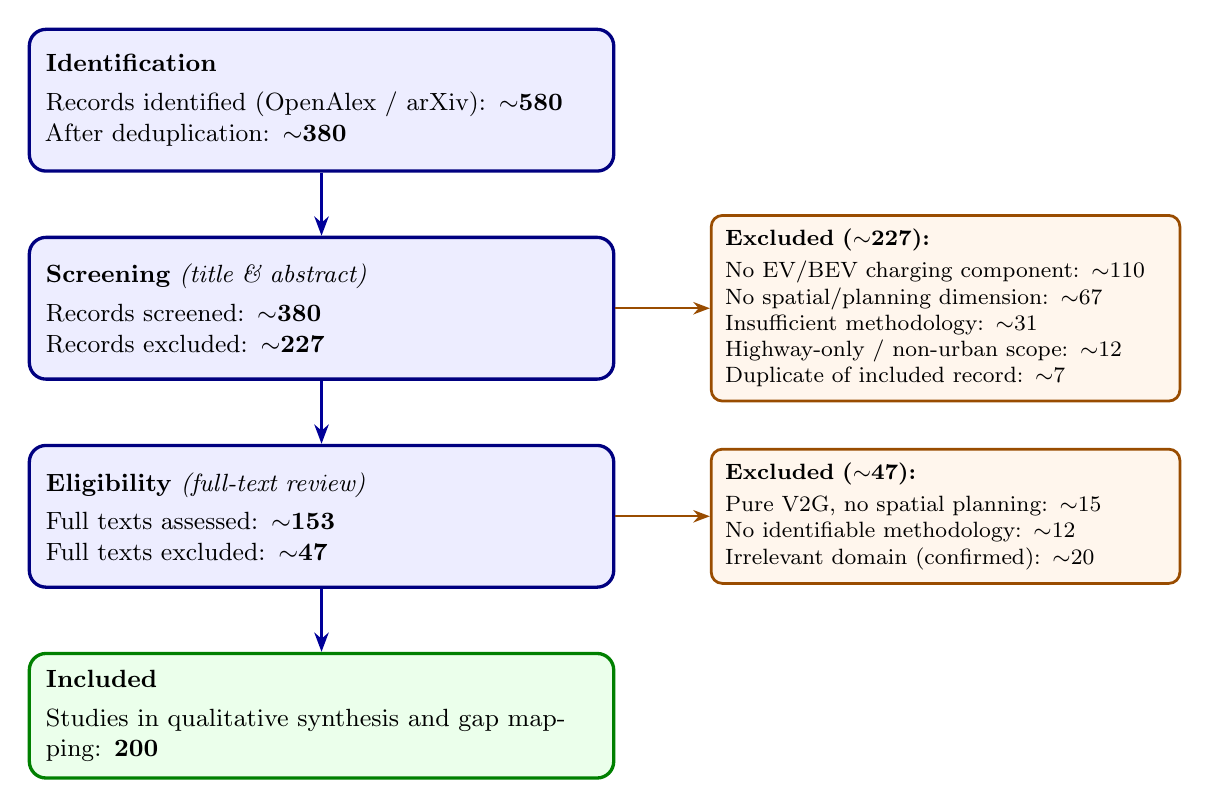
\begin{tikzpicture}[
  node distance = 8mm and 12mm,
  mainbox/.style = {
    rectangle, rounded corners=6pt,
    draw=blue!50!black, fill=blue!7, line width=1.2pt,
    text width=70mm, minimum height=18mm,
    align=left, font=\small, inner sep=6pt
  },
  inclbox/.style = {
    rectangle, rounded corners=6pt,
    draw=green!50!black, fill=green!8, line width=1.2pt,
    text width=70mm, minimum height=14mm,
    align=left, font=\small, inner sep=6pt
  },
  exclbox/.style = {
    rectangle, rounded corners=4pt,
    draw=orange!60!black, fill=orange!7, line width=1pt,
    text width=56mm, minimum height=14mm,
    align=left, font=\footnotesize, inner sep=5pt
  },
  arrow/.style  = {-{Stealth[length=7pt]}, thick, blue!60!black},
  sarrow/.style = {-{Stealth[length=6pt]}, thick, orange!60!black},
]
%% ---- Main column ----
\node[mainbox] (id) {%
  \textbf{Identification}\\[3pt]
  Records identified (OpenAlex / arXiv): \textbf{$\sim$580}\\
  After deduplication: \textbf{$\sim$380}%
};

\node[mainbox, below=of id] (screen) {%
  \textbf{Screening} \textit{(title \& abstract)}\\[3pt]
  Records screened: \textbf{$\sim$380}\\
  Records excluded: \textbf{$\sim$227}%
};

\node[mainbox, below=of screen] (elig) {%
  \textbf{Eligibility} \textit{(full-text review)}\\[3pt]
  Full texts assessed: \textbf{$\sim$153}\\
  Full texts excluded: \textbf{$\sim$47}%
};

\node[inclbox, below=of elig] (incl) {%
  \textbf{Included}\\[3pt]
  Studies in qualitative synthesis and gap mapping: \textbf{200}%
};

%% ---- Arrows between main boxes ----
\draw[arrow] (id.south)     -- (screen.north);
\draw[arrow] (screen.south) -- (elig.north);
\draw[arrow] (elig.south)   -- (incl.north);

%% ---- Exclusion box: screening ----
\node[exclbox, right=of screen] (excl1) {%
  \textbf{Excluded ($\sim$227):}\\[2pt]
  No EV/BEV charging component: $\sim$110\\
  No spatial/planning dimension: $\sim$67\\
  Insufficient methodology: $\sim$31\\
  Highway-only / non-urban scope: $\sim$12\\
  Duplicate of included record: $\sim$7%
};

%% ---- Exclusion box: eligibility ----
\node[exclbox, right=of elig] (excl2) {%
  \textbf{Excluded ($\sim$47):}\\[2pt]
  Pure V2G, no spatial planning: $\sim$15\\
  No identifiable methodology: $\sim$12\\
  Irrelevant domain (confirmed): $\sim$20%
};

%% ---- Side arrows ----
\draw[sarrow] (screen.east) -- (excl1.west);
\draw[sarrow] (elig.east)   -- (excl2.west);

\end{tikzpicture}
\caption{PRISMA 2020 flow diagram for the systematic literature review.}
\label{fig:prisma}
\end{figure}


\section{Inclusion and Exclusion Criteria}


\begin{longtable}{L{3.5cm} L{4.5cm} L{4.5cm}}
\caption{Inclusion and Exclusion Criteria}\\[4pt]
\toprule
\textbf{Type} & \textbf{Criterion} & \textbf{Rationale} \\
\midrule
\endfirsthead
\multicolumn{3}{l}{\small\textit{Table \thetable\ --- continued}}\\[2pt]
\toprule
\textbf{Type} & \textbf{Criterion} & \textbf{Rationale} \\
\midrule
\endhead
Include & Addresses EV/BEV charging infrastructure planning (not only vehicle technology) & Core domain scope \\
Include & Contains a spatial or planning dimension & Required for gap relevance \\
Include & Describes methodology with reproducible approach & Quality threshold \\
Include & English language; peer-reviewed or substantial arXiv preprint ($\geq$10 pages) & Methodological rigor \\
Include & Publication year 2011--2026 & Temporal scope \\
Exclude & Pure V2G (vehicle-to-grid) technical study without spatial planning component & Outside scope \\
Exclude & Highway-only corridor study without urban context & Outside scope \\
Exclude & Workshop abstract, poster, or conference summary without methodology detail & Insufficient detail \\
Exclude & Full text unavailable after download attempt & Practical constraint \\
Exclude & Confirmed duplicate of an included paper & Deduplication \\
\bottomrule
\end{longtable}


\section{Data Extraction}

For each included paper, structured data extraction was performed following the schema summarized in Table 2.2. The extraction schema covers 44 fields across thirteen dimensions: paper identity and metadata; research problem and scope; methodology approach and data sources; spatial unit and planning scale; demand modeling; optimization formulation; equity treatment; utilization treatment; rollout and phasing; zoning and land-use; meso-micro integration; quality assessment and limitations; and dissertation gap mapping (Gap 1--5, with evidence strings).


\begin{longtable}{L{3.5cm} L{4.5cm} L{4.5cm}}
\caption{Literature Extraction Dimensions and Analytical Purpose}\\[4pt]
\toprule
\textbf{Dimension} & \textbf{Information Extracted} & \textbf{Purpose in Analysis} \\
\midrule
\endfirsthead
\multicolumn{3}{l}{\small\textit{Table \thetable\ --- continued}}\\[2pt]
\toprule
\textbf{Dimension} & \textbf{Information Extracted} & \textbf{Purpose in Analysis} \\
\midrule
\endhead
Paper Metadata & Authors, year, venue, DOI, publication type & Enables bibliographic tracking and study categorization \\
Research Problem & Study objectives, planning scope, stated motivation & Identifies the primary challenges addressed by each study \\
Methodology & Modeling approach, datasets, computational tools & Compares methodological trends across the literature \\
Spatial Representation & Planning scale, zoning unit, spatial granularity & Evaluates how spatial structure is modeled \\
Demand Modeling & Demand estimation approach and aggregation level & Assesses how charging demand is represented \\
Optimization Framework & Objectives, constraints, optimization techniques & Compares charger placement strategies \\
Equity Considerations & Equity metrics, fairness definitions, accessibility treatment & Evaluates social equity integration \\
Utilization Modeling & Charger usage metrics and operational assumptions & Examines infrastructure utilization treatment \\
Rollout Strategy & Phased deployment and temporal planning methods & Analyzes long-term infrastructure planning \\
Zoning \& Land Use & Land-use compatibility and zoning considerations & Assesses urban planning integration \\
Meso--Micro Integration & Relationships between corridor-scale and local-scale planning & Evaluates multi-scale planning approaches \\
Research Limitations & Stated limitations and generalizability concerns & Identifies methodological weaknesses \\
Gap Mapping & Evidence related to the five identified research gaps & Supports synthesis of unresolved challenges \\
\bottomrule
\end{longtable}


Literature extraction was conducted using a two-stage process. In the first stage, bibliographic information, methodological approaches, and thematic categories were identified automatically from paper abstracts and metadata using pattern-matching techniques. In the second stage, manual verification was performed to validate research gap classifications and supporting evidence. The automated extraction process showed high agreement with manual review for methodological classification, while spatial-unit identification required additional manual verification due to inconsistent terminology across studies.

\section{Quality Assessment}

Paper quality was assessed on three dimensions: (1) methodological clarity (is the approach reproducible?); (2) data quality (are data sources described?); and (3) generalizability (are limitations stated?). Papers meeting inclusion criteria but lacking two of these three quality dimensions were retained in the review with a quality caveat noted in their extraction file.


\bigskip\noindent\rule{\linewidth}{0.4pt}\bigskip


\chapter{Related Work}

The following review organizes the literature by thematic cluster, reflecting the primary classification of each paper. Papers whose contributions span multiple themes are discussed in the section most relevant to their primary contribution and cross-referenced where appropriate. Each subsection opens with a synthetic overview of the thematic strand, followed by individual paper entries and a summary table.

\section{Spatial Optimization for Charging Station Placement}

\textit{133 papers (66\% of corpus)}

Spatial optimization constitutes the dominant methodological paradigm in charging infrastructure planning research, representing the largest thematic cluster in this review. These studies apply deterministic and stochastic mathematical programming models, principally mixed-integer linear programming (MILP), bilevel optimization, flow-based facility location formulations, and reinforcement learning, to identify optimal charging station locations subject to demand coverage, budget, and network constraints. The field has produced increasingly sophisticated formulations that incorporate traffic flow, queue dynamics, and grid capacity constraints. However, the spatial unit of analysis remains almost universally fixed to administrative boundaries, and single-period static optimization remains the norm. The richness of the optimization literature stands in contrast to its limited engagement with planning-side questions of spatial unit validity, zoning compatibility, and deployment phasing. Key contributions in this area span from classical facility location formulations applied to charging networks, to modern deep reinforcement learning approaches and data-driven placement frameworks. The following papers represent the core of this literature as identified in the systematic review.


\noindent \textbf{Najafzad et al. (2026)}~\cite{a_two-stage_2026} present \textit{A Two-Stage Stochastic Optimization Model for the Equitable Deployment of Fixed and Mobile EV Charging Stations}. A major barrier to wide adoption of Electric Vehicles (EVs) is the absence of reliable and equitable charging infrastructure. Poorly located charging stations create coverage gaps and slow down EV adoption, especially in underserved communities. This paper proposes a two-stage stochastic mixed-integer programming model for the optimal deployment of Fixed and Mobile Charging Stations (FCSs and MCSs) across multiple zones and periods. This work addresses dissertation gaps: G1, G3, G4.



\noindent \textbf{Mejia et al. (2026)}~\cite{joint_planning_2026} present \textit{Joint Planning of Distribution Systems and EV Charging Infrastructure Using a GIS-Based Spatial Analysis Framework}. This paper addresses joint planning of distribution systems and ev charging infrastructure using a gis-based spatial anal. This work addresses dissertation gaps: G1.



\noindent \textbf{Jiang et al. (2026)}~\cite{pricing_electric_2026} present \textit{Pricing EV Charging and Station Access via Copositive Duality}. Optimized charging of EVs at public locations consists of two decisions: how much energy to deliver at what times, which is continuous, and where to plug in, which is binary. This makes optimizing EV charging a MILP. This discreteness undermines traditional marginal pricing methods. This work addresses dissertation gaps: G1.



\noindent \textbf{Babur and Macfarlane (2026)} present \textit{Regional Transportation Modeling for Equitable EV Charging Infrastructure Design}. The widespread adoption of BEVs holds promise for mitigating emission-related health impacts, particularly for low-income communities disproportionately affected by exposure to traffic-related air pollution. However, designing effective charging infrastructure necessitates a regional modeling approach that accounts for the inherent cross-jurisdictional nature of mobility patterns. This study underscores the importance of regional modeling in optimizing charging station deployment and evaluating the environmental justice implications for equity priority communities. This work addresses dissertation gaps: G1, G3, G4.



\noindent \textbf{Bertucci et al. (2026)}~\cite{simultaneous_optimization_2026} present \textit{Simultaneous Optimization of Electric Ferry Operations and Charging Infrastructure}. Electrification of marine transport is a promising solution to reduce sector greenhouse gas emissions and operational costs. However, the large upfront cost of electric vessels and the required charging infrastructure can be a barrier to the development of this technology. Optimization algorithms that jointly design the charging infrastructure and the operation of electric vessels can help to reduce these costs and make these projects viable. This work addresses dissertation gaps: G1.



\noindent \textbf{Fariza et al. (2026)}~\cite{strategic_planning_2026} present \textit{Strategic Planning of Public EV Charging Stations Using AHP and GIS to Support Sustainable Mobility in West Java, Indonesia}. The transition toward sustainable and low-emission transportation in Indonesia has accelerated the adoption of EVs, especially in densely populated provinces such as West Java. Despite this progress, the distribution and capacity of Public EV Charging Stations (EVCS) remain uneven, creating significant gaps between vehicle growth and infrastructure readiness. This spatial imbalance threatens to slow down EV adoption and limit the effectiveness of national decarbonization targets. This work addresses dissertation gaps: G1, G2.



\noindent \textbf{Do et al. (2025)}~\cite{a_2025} present \textit{A Digital Twin Framework for Decision-Support and Optimization of EV Charging Infrastructure in Localized Urban Systems}. As EV adoption accelerates in urban environments, optimizing charging infrastructure is vital for balancing user satisfaction, energy efficiency, and financial viability. This study advances beyond static models by proposing a digital twin framework that integrates agent-based decision support with embedded optimization to dynamically simulate EV charging behaviors, infrastructure layouts, and policy responses across scenarios. Applied to a localized urban site (a university campus) in Hanoi, Vietnam, the model evaluates operational policies, EV station configurations, and renewable energy sources. This work addresses dissertation gaps: G1, G5.



\noindent \textbf{Ameer et al. (2025)}~\cite{hybrid_optimization_2025} present \textit{A density-based spatial clustering and linear programming method for EV charging station location and price optimization}. This paper addresses a density-based spatial clustering and linear programming method for EV charging stati. This work addresses dissertation gaps: G1.



\noindent \textbf{Yu et al. (2025)}~\cite{a_joint_2025} present \textit{A Joint Planning Model for Fixed and Mobile EV Charging Stations Considering Flexible Capacity Strategy}. The widespread adoption of EVs has significantly increased demand on both transportation and power systems, posing challenges to their stable operation. To support the growing need for EV charging, both fixed charging stations (FCSs) and mobile charging stations (MCSs) have been introduced, serving as key interfaces between the power grid and traffic network. Recognizing the importance of collaborative planning across these sectors, this paper presents a two-stage joint planning model for FCSs and MCSs, utilizing an improved alternating direction method of multipliers (ADMM) algorithm. This work addresses dissertation gaps: G1, G4.



\noindent \textbf{Karaku\c{s} and Corcoran (2025)} present \textit{A Multi-Modal Spatial Risk Framework for EV Charging Infrastructure Using Remote Sensing}. EV charging infrastructure is increasingly critical to sustainable transport systems, yet its resilience under environmental and infrastructural stress remains underexplored. In this paper, we introduce RSERI-EV, a spatially explicit and multi-modal risk assessment framework that combines remote sensing data, open infrastructure datasets, and spatial graph analytics to evaluate the vulnerability of EV charging stations. RSERI-EV integrates diverse data layers, including flood risk maps, land surface temperature (LST) extremes, vegetation indices (NDVI), land use/land cover (LULC), proximity to electrical substations, and road accessibility to generate a composite Resilience Score. This work addresses dissertation gaps: G1, G2, G4.



\noindent \textbf{Huang et al. (2025)}~\cite{a_spatially_2025} present \textit{A Spatially Aware Machine Learning Method for Locating EVCSs}. The rapid adoption of EVs has driven a strong need for optimizing locations of electric vehicle charging stations (EVCSs). Previous methods for locating EVCSs rely on statistical and optimization models, but these methods have limitations in capturing complex nonlinear relationships and spatial dependencies among factors influencing EVCS locations. To address this research gap and better understand the spatial impacts of urban activities on EVCS placement, this study presents a spatially aware machine learning (SAML) method that combines a multi-layer perceptron (MLP) model with a spatial loss function to optimize EVCS sites. This work addresses dissertation gaps: G1.



\noindent \textbf{Meng et al. (2025)}~\cite{a_two-stage_2025} present \textit{A two-stage optimization framework for EV charging station planning considering investment cost and service satisfaction}. This paper addresses a two-stage optimization framework for ev charging station planning considering investment cost and . This work addresses dissertation gaps: G1.



\noindent \textbf{Kinchen et al. (2025)}~\cite{a_united_2025} present \textit{A United Framework for Planning EV Charging Accessibility}. The shift towards EVs is crucial for establishing sustainable and low-emission urban transportation systems. However, the success of this transition depends on the strategic placement of the charging infrastructure. This paper addresses the challenge of optimizing charging station locations in dense urban environments while balancing efficiency with spatial accessibility. This work addresses dissertation gaps: G1, G3.



\noindent \textbf{Nankali and Levin (2025)} present \textit{An Exact Solution Algorithm for the Bi-Level Optimization Problem of EVs Charging Station Placement}. This work addresses EV charging station placement through a bi-level optimization model, where the upper-level planner maximizes net revenue by selecting station locations under budget constraints, while EV users at the lower level choose routes and charging stations to minimize travel and charging costs. To account for range anxiety, we construct a battery-expanded network and apply a shortest path algorithm with Frank-Wolfe traffic assignment. Our primary contribution is developing the first exact solution algorithm for large scale EV charging station placement problems. This work addresses dissertation gaps: G1.



\noindent \textbf{Mousaei (2025)}~\cite{analyzing_locational_2025} present \textit{Analyzing locational inequalities in the placement of EVCSs using machine learning: A case study in Glasgow}. This paper addresses analyzing locational inequalities in the placement of EVCSs using machi. This work addresses dissertation gaps: G1.



\noindent \textbf{Silva et al. (2025)}~\cite{causal_spillover_2025} present \textit{Causal spillover effects of EVCS placement on local businesses: a staggered adoption study}. Understanding the economic impacts of the placement of EVCSs is crucial for planning infrastructure systems that benefit the broader community. Theoretical models have been used to predict human behavior during charging events, however, these models have often neglected the complexity of trip patterns, and have underestimated the real-world impacts of such infrastructure on the local economy. In this paper, we design a quasi-experiment using mobile phone GPS location and EVCS deployment history data to analyze the causal impact of EVCS placement on visitation patterns to businesses. This work addresses dissertation gaps: G1, G4.



\noindent \textbf{Islam et al. (2025)}~\cite{charge-map_an_2025} present \textit{CHARGE-MAP: An integrated framework to study the multicriteria EV charging infrastructure expansion problem}. The widespread adoption of EVs in recent years has necessitated the development of effective charging infrastructures. However, charging infrastructure expansion is a multifaceted problem that requires careful consideration of the existing infrastructure, spatiotemporal distribution of charging demands, power-grid capacity, and budget constraints. To approach this complex problem, we present charge-map , a data-driven simulation-optimization framework, focused on ensuring meaningful charging experience for individual EV owners. This work addresses dissertation gaps: G1, G4.



\noindent \textbf{Nguyen et al. (2025)}~\cite{competitive_ev_2025} present \textit{Competitive EV charging station location with queues}. EV public charging infrastructure planning faces significant challenges in competitive markets, where multiple service providers affect congestion and user behavior. This work extends existing modeling frameworks by incorporating the presence of competitors' stations and more realistic queueing systems. First, we analyze three finite queueing systems, M/M/1/K, M/M/s/K, and M/Er/s/K, with varying numbers of servers (charging outlets) and service time distributions, deriving analytic expressions for user behavior metrics. This work addresses dissertation gaps: G1.



\noindent \textbf{Alharbi et al. (2025)}~\cite{data-driven_ev_2025} present \textit{Data-driven EV charging infrastructure with uncertainty based on a spatial--temporal flow-driven (STFD) models considering batteries}. This paper addresses data-driven ev charging infrastructure with uncertainty based on a spatial--temporal flow-driven (stf. This work addresses dissertation gaps: G1, G4.



\noindent \textbf{Junker et al. (2025)}~\cite{data-driven_optimization_2025} present \textit{Data-Driven Optimization of EV Charging Station Placement Using Causal Discovery}. This paper addresses the critical challenge of optimizing EVCS placement through a novel data-driven methodology employing causal discovery techniques. While traditional approaches prioritize economic factors or power grid constraints, they often neglect empirical charging patterns that ultimately determine station utilization. We analyze extensive charging data from Palo Alto and Boulder (337,344 events across 100 stations) to uncover latent relationships between station characteristics and utilization. This work addresses dissertation gaps: G1.



\noindent \textbf{Zhao et al. (2025)}~\cite{electric_vehicle_2025} present \textit{EV Charging Planning: A Complex Systems Perspective}. This paper addresses EV charging planning: a complex systems perspective. This work addresses dissertation gaps: G1, G3.



\noindent \textbf{Kapoor (2025)}~\cite{explainable_and_2025} present \textit{Explainable and context-aware Graph Neural Networks for dynamic EV route optimization to optimal charging station}. This paper addresses explainable and context-aware graph neural networks for dynamic EV route optimization . This work addresses dissertation gaps: G1.



\noindent \textbf{Yuan et al. (2025)}~\cite{planning_future_2025} present \textit{Fairness-Oriented Charging Station Location Optimization Driven by Deep Reinforcement Learning}. This paper addresses fairness-oriented charging station location optimization driven by deep reinforcement learning. This work addresses dissertation gaps: G1, G3.



\noindent \textbf{Ameer et al. (2025)}~\cite{hybrid_optimization_2025} present \textit{Hybrid optimization of EV charging station placement and pricing using Bender?s decomposition and NSGA-II algorithm}. This paper addresses hybrid optimization of ev charging station placement and pricing using bender?s decomposition and ns. This work addresses dissertation gaps: G1.



\noindent \textbf{Okada et al. (2025)}~\cite{joint_optimization_2025} present \textit{Joint Optimization of EV Routes and Charging Locations Learning Charge Constraints Using QUBO Solver}. Optimal routing problems of EVs have attracted much attention in recent years, and installation of charging stations is an important issue for EVs. Hence, we focus on the joint optimization of the location of charging stations and the routing of EVs. When routing problems are formulated in the form of quadratic unconstrained binary optimization (QUBO), specialized solvers such as quantum annealer are expected to provide optimal solutions with high speed and accuracy. This work addresses dissertation gaps: G1, G4.



\noindent \textbf{Zheng et al. (2025)}~\cite{large_language_2025} present \textit{Large Language Model-Assisted Planning of EV Charging Infrastructure with Real-World Case Study}. The growing demand for EV charging infrastructure presents significant planning challenges, requiring efficient strategies for investment and operation to deliver cost-effective charging services. However, the potential benefits of EV charging assignment, particularly in response to varying spatial-temporal patterns of charging demand, remain under-explored in infrastructure planning. This paper proposes an integrated approach that jointly optimizes investment decisions and charging assignments while accounting for spatial-temporal demand dynamics and their interdependencies. This work addresses dissertation gaps: G1, G4.



\noindent \textbf{Choi et al. (2025)}~\cite{location_and_2025} present \textit{Location and capacity optimization of EV charging stations using genetic algorithms and fuzzy analytic hierarchy process}. This paper addresses location and capacity optimization of ev charging stations using genetic algorithms and fuzzy analyt. This work addresses dissertation gaps: G1.



\noindent \textbf{Ruiz-Barajas et al. (2025)}~\cite{multiobjective_model_2025} present \textit{Multiobjective model to optimize charging station location for the decarbonization process in Mexico}. EVs offer significant potential for advancing sustainable environmental goals. However, their widespread adoption has been concentrated in urban areas, raising challenges for interurban travel. In many countries, charging station networks are primarily located within cities, highlighting a key opportunity for expansion to support longer distance journeys. This work addresses dissertation gaps: G1.



\noindent \textbf{Nakao et al. (2025)}~\cite{optimal_mixed_2025} present \textit{Optimal mixed fleet and charging infrastructure planning to electrify demand responsive feeder services with target CO2 emission constraints}. Electrifying demand-responsive transport systems need to plan the charging infrastructure carefully, considering the trade-offs of charging efficiency and charging infrastructure costs. Earlier studies assume a fully electrified fleet and overlook the planning issue in the transition period. This study addresses the joint fleet size and charging infrastructure planning for a demand-responsive feeder service under stochastic demand, given a user-defined targeted CO2 emission reduction policy. This work addresses dissertation gaps: G1.



\noindent \textbf{Zhang et al. (2025)}~\cite{optimization_of_2025} present \textit{Optimization of EVCS Location Distribution Based on Activity--Travel Patterns}. With the rapid expansion of the EV market, optimizing the distribution of charging stations has attracted increasing attention. Unlike internal combustion engine vehicles, EVs are typically charged at the end of a trip rather than during transit. Therefore, analyzing EV users? charging preferences based on their activity--travel patterns is essential. This work addresses dissertation gaps: G1.



\noindent \textbf{Zhong et al. (2025)}~\cite{optimizing_electric_2025} present \textit{Optimizing electric bus charging station locations: An integrated land-use and transportation approach}. This paper addresses optimizing electric bus charging station locations: an integrated land-use and transportation approa. This work addresses dissertation gaps: G1.



\noindent \textbf{Ai et al. (2025)}~\cite{optimizing_urban_2025} present \textit{Optimizing Urban EV Charging and Battery Swapping Infrastructure: A Location-Inventory-Grid Model}. The rapid rise of EVs places unprecedented stress on both urban mobility systems and low-voltage power grids. Designing battery swapping and charging networks that are cost-efficient, grid-compatible, and sustainable is therefore a pressing yet complex challenge: service providers must jointly optimize station locations, battery inventory, and grid interaction under high-dimensional uncertainty. We develop an integrated location-inventory-grid model and employ a continuous approximation approach to overcome the intractability of discrete formulations. This work addresses dissertation gaps: G1, G5.



\noindent \textbf{Yuan et al. (2025)}~\cite{planning_future_2025} present \textit{Planning future charging infrastructure for private EVs: A city-scale assessment of demand and capacity}. This study proposes the first demand-driven, multi-objective planning model for optimizing city-scale capacity allocation of EV charging infrastructure. The model employs a bottom-up approach to estimate charging demand differentiated by vehicle type-BEVs, extended-range EVs (EREVs), and plug-in hybrid EVs (PHEVs). Chongqing, a rapidly expanding EV industry cluster in China with a strong industrial base, supportive policies, and diverse urban morphologies, is selected as the case study. This work addresses dissertation gaps: G1, G4.



\noindent \textbf{Mousaei and Naderi (2025)} present \textit{Predicting Optimal Placement of EV Charge Stations Using Machine Learning: A Case Study in Glasgow, UK}. This paper addresses predicting optimal placement of EV charge stations using machine learning: a case stud. This work addresses dissertation gaps: G1.



\noindent \textbf{Zhu et al. (2025)}~\cite{reinforcement_learning_2025} present \textit{Reinforcement Learning for Hybrid Charging Stations Planning and Operation Considering Fixed and Mobile Chargers}. The success of vehicle electrification relies on efficient and adaptable charging infrastructure. Fixed-location charging stations often suffer from underutilization or congestion due to fluctuating demand, while mobile chargers offer flexibility by relocating as needed. This paper studies the optimal planning and operation of hybrid charging infrastructures that combine both fixed and mobile chargers within urban road networks. This work addresses dissertation gaps: G1.



\noindent \textbf{Xia et al. (2025)}~\cite{robust_charging_2025} present \textit{Robust charging station location and routing-scheduling for electric modular autonomous units}. Problem definition: Motivated by global electrification targets and the advent of electric modular autonomous units (E-MAUs), this paper addresses a robust charging station location and routing-scheduling problem (E-RCRSP) in an inter-modal transit system, presenting a novel solution to traditional electric bus scheduling. The system integrates regular bus services, offering full-line or sectional coverage, and short-turning services. Considering the fast-charging technology with quick top-ups, we jointly optimize charging station locations and capacities, fleet sizing, as well as routing-scheduling for E-MAUs under demand uncertainty. This work addresses dissertation gaps: G1.




\noindent \textbf{Ju et al. (2025)}~\cite{trajectory-integrated_accessibility_2025} present \textit{Trajectory-Integrated Accessibility Analysis of Public EVCSs}. EV charging infrastructure is crucial for advancing EV adoption, managing charging loads, and ensuring equitable transportation electrification. However, there remains a notable gap in comprehensive accessibility metrics that integrate the mobility of the users. This study introduces a novel accessibility metric, termed Trajectory-Integrated Public EVCS Accessibility (TI-acs), and uses it to assess public EVCS accessibility for approximately 6 million residents in the San Francisco Bay Area based on detailed individual trajectory data in one week. This work addresses dissertation gaps: G1.



\noindent \textbf{Zhang and Tan (2024)} present \textit{A data-driven approach of layout evaluation for EV charging infrastructure using agent-based simulation and GIS}. The development and popularization of new energy vehicles have become a global consensus. The shortage and unreasonable layout of EV charging infrastructure (EVCI) have severely restricted the development of EVs. In the literature, many methods can be used to optimize the layout of charging stations (CSs) for producing good layout designs. This work addresses dissertation gaps: G1, G4, G5.



\noindent \textbf{Zhang and Shi (2024)} present \textit{A multi-objective site selection of EVCS based on NSGA-II}. The planning of charging infrastructure is crucial to developing EVs. Planning for charging stations requires considering several variables, including building costs, charging demand, and coverage levels. It might be advantageous to use a multi-objective optimization method based on the NSGA-II. This work addresses dissertation gaps: G1, G2.



\noindent \textbf{Aljaidi et al. (2024)}~\cite{a_particle_2024} present \textit{A particle swarm optimizer-based optimization approach for locating EVs charging stations in smart cities}. This paper addresses a particle swarm optimizer-based optimization approach for locating EVs charging stati. This work addresses dissertation gaps: G1.



\noindent \textbf{Radvand et al. (2024)}~\cite{a_quantum_2024} present \textit{A Quantum Optimization Algorithm for Optimal EVCS Placement for Intercity Trips}. EVs play a significant role in enhancing the sustainability of transportation systems. However, their widespread adoption is hindered by inadequate public charging infrastructure, particularly to support long-distance travel. Identifying optimal charging station locations in large transportation networks presents a well-known NP-hard combinatorial optimization problem, as the search space grows exponentially with the number of potential charging station locations. This work addresses dissertation gaps: G1.



\noindent \textbf{Wu et al. (2024)}~\cite{allocate_electric_2024} present \textit{A two-layer planning method for location and capacity determination of public EVCSs}. This paper addresses a two-layer planning method for location and capacity determination of public EV charg. This work addresses dissertation gaps: G1.



\noindent \textbf{Zhang et al. (2024)}~\cite{a_multi-objective_2024} present \textit{Advancing urban EVCSs: AI-driven day-ahead optimization of pricing and Nudge strategies utilizing multi-agent deep reinforcement learning}. This paper addresses advancing urban EVCSs: ai-driven day-ahead optimization of pricing and . This work addresses dissertation gaps: G1.



\noindent \textbf{Liu et al. (2024)}~\cite{battery_swapping_2024} present \textit{BSS location for EVs: a simulation optimization approach}. EVs face significant energy supply challenges due to long charging times and congestion at charging stations. Battery swapping stations (BSSs) offer a faster alternative for energy replenishment, but their deployment costs are considerably higher than those of charging stations. As a result, selecting optimal locations for BSSs is crucial to improve their accessibility and utilization. This work addresses dissertation gaps: G1, G4.



\noindent \textbf{Wang and Lin (2024)}~\cite{planning_of_2024} present \textit{Beyond Profit: A Multi-Objective Framework for EVCS Operations}. This paper explores the pricing and scheduling strategies of the EVCSs in response to the rising demand for cleaner transportation. Most of the existing methods focus on maximizing the energy efficiency or the charging station profit, however, the reputation of EVs is also a key factor for the long-term charging station operations. To address these gaps, we propose a novel framework for jointly optimizing pricing and continuous-multiple charging rates. This work addresses dissertation gaps: G1.



\noindent \textbf{Cai et al. (2024)}~\cite{charging_station_2024} present \textit{Charging Station Site Selection Optimization for Electric Logistics Vehicles, Taking into Account Time-Window and Load Constraints}. In order to improve the efficiency of the ?last-mile? distribution in urban logistics and solve the problem of the difficult charging of electric logistics vehicles (ELVs), this paper proposes a charging station location optimization scheme for ELVs that takes into account time-window and load constraints (TW-LCs). Taking the optimal transportation path as the objective function and considering the time-window and vehicle load constraints, a charging station siting model was established. For the TW-LC problem, an improved genetic algorithm combining the farthest-insertion heuristic idea and local search operation was designed. This work addresses dissertation gaps: G1.



\noindent \textbf{Li et al. (2024)}~\cite{electric_vehicle_2024} present \textit{EV Charging Infrastructure Optimization Incorporating Demand Forecasting and Renewable Energy Application}. The rapid growth in EV adoption and the increasing use of renewable energy have introduced challenges in designing and managing EV charging infrastructure. This study presents a framework that combines a hybrid deep learning model, spatial and temporal demand analysis, and vehicle-to-grid (V2G) optimization to address these issues. The framework achieved high predictive accuracy, with an RMSE of 2.1 kWh and an R2R\^\{\}2R2 value of 0.92, effectively capturing daily demand patterns and variations across charging stations. This work addresses dissertation gaps: G1.



\noindent \textbf{Cao and Zhou (2024)} present \textit{Energy management optimization of hybrid EVs based on deep learning model predictive control}. In this paper, the hybrid EV (HEV) energy management optimization method is proposed based on deep learning (DL) model predictive control. Through empirical research combined with the questionnaire survey, this article not only provides a new perspective and practical basis but also improves the efficiency and accuracy of the model by improving the relevant algorithms. The study first analyzes the importance of HEV energy management and reviews the existing literature. This work addresses dissertation gaps: G1.



\noindent \textbf{Mehditabrizi et al. (2024)}~\cite{integrating_en_2024} present \textit{Integrating En Route and Home Proximity in EV Charging Accessibility: A Spatial Analysis in the Washington Metropolitan Area}. This study evaluates the accessibility of public EV charging stations in the Washington metropolitan area using a comprehensive measure that accounts for both destination-based and en route charging opportunities. By incorporating the full spectrum of daily travel patterns into the accessibility evaluation, our methodology offers a more realistic measure of charging opportunities than destination-based methods that prioritize proximity to residential locations. Results from spatial autocorrelation analysis indicate that conventional accessibility assessments often overestimate the availability of infrastructure in central urban areas and underestimate it in peripheral commuting zones, potentially leading to misallocated resources. This work addresses dissertation gaps: G1.



\noindent \textbf{Mohammed et al. (2024)}~\cite{multiobjective_optimization_2024} present \textit{Multiobjective optimization for sizing and placing EVCSs considering comprehensive uncertainties}. This paper addresses multiobjective optimization for sizing and placing EVCSs considering co. This work addresses dissertation gaps: G1.



\noindent \textbf{Kumar and Channi (2024)}~\cite{optimizing_electric_2024} present \textit{Optimal EVCS Placement: A Multi-Criteria Decision-Making Approach for Site Selection}. This paper addresses optimal EVCS placement: a multi-criteria decision-making approach for s. This work addresses dissertation gaps: G1.



\noindent \textbf{Pierrou et al. (2024)}~\cite{optimal_ev_2024} present \textit{Optimal EV Charging Scheduling at Electric Railway Stations Under Peak Load Constraints}. In this paper, a novel Energy Management System (EMS) algorithm to achieve optimal EV charging scheduling at the parking lots of electric railway stations is proposed. The proposed approach uncovers the potential of leveraging EV charging flexibility to prevent overloading in the combined EV charging and railway operation along with renewable generation, railway regenerative capabilities, and energy storage. Specifically, to realize end-user flexibility, each EV state of charge at departure time is introduced as an optimization variable. This work addresses dissertation gaps: G1.



\noindent \textbf{He et al. (2024)}~\cite{optimal_evcs_2024} present \textit{Optimal EVCS planning via spatial-temporal distribution of charging demand forecasting and traffic-grid coupling}. This paper addresses optimal evcs planning via spatial-temporal distribution of charging demand forecasting and traffic-g. This work addresses dissertation gaps: G1, G4.



\noindent \textbf{Heo and Chang (2024)} present \textit{Optimal planning for EV fast charging stations placements in a city scale using an advantage actor-critic deep reinforcement learning and geospatial analysis}. This paper addresses optimal planning for EV fast charging stations placements in a city scale using an adv. This work addresses dissertation gaps: G1.



\noindent \textbf{Panyaram (2024)}~\cite{optimization_strategies_2024} present \textit{Optimization Strategies for Efficient Charging Station Deployment in Urban and Rural Networks}. Optimized charging station deployment will enrich the EV ecosystem, especially in diversified urban and rural environments. In this research paper, an effort has been made to optimization strategies regarding the location of EV charging stations and how these can be operated effectively. The study analyzes key factors, such as population density, travel patterns, energy demand, and land availability, that provide a comprehensive framework for policymakers and planners. This work addresses dissertation gaps: G1, G4.



\noindent \textbf{Huang and Zhou (2024)} present \textit{Optimizing EV Charging Station Placement in New South Wales: A Soft Actor-Critic Reinforcement Learning Approach}. This paper addresses optimizing ev charging station placement in new south wales: a soft actor-critic reinforcement learn. This work addresses dissertation gaps: G1.



\noindent \textbf{Munawar (2024)}~\cite{optimizing_urban_2024} present \textit{Optimizing Urban Logistics Through EV Integration}. The transition to electric-based logistics has become increasingly vital in the pursuit of sustainable urban transportation. This study presents a narrative review of recent literature examining the efficiency, environmental impact, and policy dimensions of EV adoption in logistics. Drawing on peer-reviewed articles from Scopus and Google Scholar published between 2015 and 2024, this review employed systematic keyword searches and thematic analysis to synthesize research findings. This work addresses dissertation gaps: G1, G5.



\noindent \textbf{Shen et al. (2024)}~\cite{sequential_charging_2024} present \textit{Sequential Charging Station Location Optimization under Uncertain Charging Behavior and User Growth}. Charging station availability is crucial for a thriving EV market. Due to budget constraints, locating these stations usually proceeds in phases, which calls for careful consideration of the (random) charging demand growth throughout the planning horizon. This paper integrates user choice behavior into two-stage and multi-stage stochastic programming models for intracity charging station planning under demand uncertainty. This work addresses dissertation gaps: G1, G4.



\noindent \textbf{Seilabi et al. (2024)}~\cite{sustainable_planning_2024} present \textit{Sustainable Planning of EVCSs: A Bi-Level Optimization Framework for Reducing Vehicular Emissions in Urban Road Networks}. This paper proposes a decision-making framework for a multiple-period planning of EV charging station development. In this proposed framework, transportation planners seek to implement a phased provision of electric charging stations as well as repurposing gas stations at selected locations. The developed framework is presented as a bi-level optimization problem that determines the optimal electric charging network design while capturing the practical constraints and travelers? decisions. This work addresses dissertation gaps: G1, G4.



\noindent \textbf{Akbay et al. (2024)}~\cite{the_electric_2024} present \textit{The EV Problem with Road Junctions and Road Types: An Ant Colony Optimization Approach}. This paper addresses the EV problem with road junctions and road types: an ant colony optimization approach. This work addresses dissertation gaps: G1.



\noindent \textbf{Boonprong et al. (2024)}~\cite{towards_sustainable_2024} present \textit{Towards Sustainable Urban Mobility: Voronoi-Based Spatial Analysis of EV Charging Stations in Bangkok}. This study leverages the efficacy of Voronoi diagram theory within a mixed-methods approach to thoroughly examine the spatial distribution, service coverage, and optimal locations for expanding EV charging infrastructure in Bangkok. Drawing on data from field surveys and public data providers, our analysis unfolds in four key stages. Firstly, we delve into the spatial distribution of charging stations, scrutinizing density, proximity to various road types, and land use through the lens of Voronoi diagrams. This work addresses dissertation gaps: G1, G2, G3.



\noindent \textbf{Miltner et al. (2024)}~\cite{towards_using_2024} present \textit{Towards Using Machine Learning to Generatively Simulate EV Charging in Urban Areas}. This study addresses the challenge of predicting EV charging profiles in urban locations with limited data. Utilizing a neural network architecture, we aim to uncover latent charging profiles influenced by spatio-temporal factors. Our model focuses on peak power demand and daily load shapes, providing insights into charging behavior. This work addresses dissertation gaps: G1, G4.



\noindent \textbf{Alhussan et al. (2024)}~\cite{urban_electric_2024} present \textit{Urban EVCS Placement Optimization with Graylag Goose Optimization Voting Classifier}. This paper addresses urban EVCS placement optimization with graylag goose optimization votin. This work addresses dissertation gaps: G1.



\noindent \textbf{Xin et al. (2023)}~\cite{a_battery_2023} present \textit{A BEV Transportation Network Design Model with Bounded Rational Travelers}. With governments worldwide emphasizing environmental protection and the global focus on carbon reduction, the BEV industry has developed rapidly. An urban transportation network with BEVs as the main form of transportation will soon become mainstream. Motivated by the abovementioned background, a BEV transportation network design problem is investigated, and a network design model is established. This work addresses dissertation gaps: G1.



\noindent \textbf{Al-Dahabreh et al. (2023)}~\cite{a_data-driven_2023} present \textit{A Data-Driven Framework for Improving Public EV Charging Infrastructure: Modeling and Forecasting}. This work presents an investigation and assessment framework, which, supported by realistic data, aims at provisioning operators with in-depth insights into the consumer-perceived Quality-of-Experience (QoE) at public EV charging infrastructures. Motivated by the unprecedented EV market growth, it is suspected that the existing charging infrastructure will soon be no longer capable of sustaining the rapidly growing charging demands; let alone that the currently adopted ad hoc infrastructure expansion strategies seem to be far from contributing any quality service sustainability solutions that tangibly reduce (ultimately mitigate) the severity of this problem. Without suitable QoE metrics, operators, today, face remarkable difficulty in assessing the performance of EV Charging Stations (EVCSs) in this regard. This work addresses dissertation gaps: G1.



\noindent \textbf{Arief et al. (2023)}~\cite{a_robust_2023} present \textit{A Robust and Efficient Optimization Model for EVCSs in Developing Countries under Electricity Uncertainty}. The rising demand for EVs worldwide necessitates the development of robust and accessible charging infrastructure, particularly in developing countries where electricity disruptions pose a significant challenge. Earlier charging infrastructure optimization studies do not rigorously address such service disruption characteristics, resulting in suboptimal infrastructure designs. To address this issue, we propose an efficient simulation-based optimization model that estimates candidate stations' service reliability and incorporates it into the objective function and constraints. This work addresses dissertation gaps: G1, G3.



\noindent \textbf{Yi et al. (2023)}~\cite{an_agent-based_2023} present \textit{An agent-based modeling approach for public charging demand estimation and charging station location optimization at urban scale}. This paper addresses an agent-based modeling approach for public charging demand estimation and charging station location. This work addresses dissertation gaps: G1.



\noindent \textbf{Varma et al. (2023)}~\cite{electric_vehicle_2023} present \textit{EV Fleet and Charging Infrastructure Planning}. We study EV fleet and charging infrastructure planning in a spatial setting. With customer requests arriving continuously at rate $\lambda$ throughout the day, we determine the minimum number of vehicles and chargers for a target service level, along with matching and charging policies. While non-EV systems require extra $\Theta(\lambda^{2/3})$ vehicles due to pickup times, EV systems differ. This work addresses dissertation gaps: G1, G5.



\noindent \textbf{Qiao et al. (2023)}~\cite{fast-charging_station_2023} present \textit{Fast-charging station location problem: A two-phase approach with mathematical program with equilibrium constraints considering charging choice behaviour}. This paper addresses fast-charging station location problem: a two-phase approach with mathematical program with equilibr. This work addresses dissertation gaps: G1.



\noindent \textbf{Filippi et al. (2023)}~\cite{incorporating_time-dependent_2023} present \textit{Incorporating time-dependent demand patterns in the optimal location of capacitated charging stations}. A massive use of EVs is nowadays considered to be a key element of a sustainable transportation policy and the availability of charging stations is a crucial issue for their extensive use. Charging stations in an urban area have to be deployed in such a way that they can satisfy a demand that may dramatically vary in space and time. In this paper we present an optimization model for the location of charging stations that takes into account the main specific features of the problem, in particular the different charging technologies, and their associated service time, and the fact that the demand depends on space and time. This work addresses dissertation gaps: G1, G4.



\noindent \textbf{Tambunan et al. (2023)}~\cite{initial_location_2023} present \textit{Initial location selection of EVs charging infrastructure in urban city through clustering algorithm}. Transportation is one of the critical sectors worldwide, mainly based on fossil fuels, especially internal combustion engines. In a developing country, heightened dependence on fossil fuels affected energy sustainability issues, greenhouse gas emissions, and increasing state budget allocation towards fuel subsidies. Moreover, shifting to EVs with alternative energy, primely renewable energy sources, is considered a promising alternative to decreasing dependence on fossil fuel consumption. This work addresses dissertation gaps: G1.



\noindent \textbf{Jiang (2023)}~\cite{layout_and_2023} present \textit{Layout and optimization of charging piles for new energy EVs -- A study on Xi'an urban area}. This paper analyzes the current layout of public charging stations within the third ring road of Xi'an central urban area and the daily charging needs of residents, the main problems in the layout of EVCSs in the central urban area of Xi'an were found, the differentiated demand analysis of living space charging was carried out, and the location model of EV public charging station facilities in the central urban area of the city was constructed, the location selection and optimization of EV public charging stations in the central urban area of Xi'an were studied. At the same time, a reasonable pile configuration was carried out, finally, the layout scheme of EV public charging stations in the central urban area was formed, the main shortcomings of the current charging pile layout and the factors (demand side) that should be considered in the current and future charging pile layout are concluded, and the layout and optimization of charging piles for clean energy in the future are prospected. This work addresses dissertation gaps: G1.



\noindent \textbf{Parent et al. (2023)}~\cite{maximum_flow-based_2023} present \textit{Maximum flow-based formulation for the optimal location of EVCSs}. With the increasing effects of climate change, the urgency to step away from fossil fuels is greater than ever before. EVs are one way to diminish these effects, but their widespread adoption is often limited by the insufficient availability of charging stations. In this work, our goal is to expand the infrastructure of EV charging stations, in order to provide a better quality of service in terms of user satisfaction (and availability of charging stations). This work addresses dissertation gaps: G1, G4.



\noindent \textbf{Tiu et al. (2023)}~\cite{on_the_2023} present \textit{On the Optimal Placement of EVCSs}. Increasing the adoption of EV is an integral part of many strategies to address climate change and air pollution. However, EV adoption rates are inhibited by several factors which reduce the confidence of potential buyers of EVs, namely range anxiety and limited charging infrastructure. The latter concern can be addressed by carefully planning the placement of EVCSs to sustainably meet long-term demand. This work addresses dissertation gaps: G1, G4.



\noindent \textbf{Mourgues et al. (2023)}~\cite{optimal_location_2023} present \textit{Optimal Location of EVs Public Charging Stations Based on a Macroscopic Urban Electromobility Model}. This paper addresses optimal location of evs public charging stations based on a macroscopic urban electromobility model. This work addresses dissertation gaps: G1.



\noindent \textbf{Liu et al. (2023)}~\cite{optimal_placement_2023} present \textit{Optimal Placement of Charging Stations in Road Networks: A Reinforcement Learning Approach with Attention Mechanism}. With the aim of promoting energy conservation and emission reduction, EVs have gained significant attention as a strategic industry in many countries. However, the insufficiency of accessible charging infrastructure remains a challenge, hindering the widespread adoption of EVs. To address this issue, we propose a novel approach to optimize the placement of charging stations within a road network, known as the charging station location problem (CSLP). This work addresses dissertation gaps: G1, G3.



\noindent \textbf{Wu et al. (2023)}~\cite{optimizing_electric_2023} present \textit{Optimizing EV Charging Infrastructure on Highways: A Multi-Agent-Based Planning Approach}. The lack of sufficient charging infrastructure for long-haul transportation is a significant barrier preventing the widespread adoption of EVs. Planning EV charging facilities in this context requires considerations distinct from those in urban environments, accounting for factors such as traffic patterns and charging behaviors. This research paper presents a multi-agent simulation model designed to assess travel and charging activities, specifically on highways. This work addresses dissertation gaps: G1.



\noindent \textbf{Pal et al. (2023)}~\cite{placement_of_2023} present \textit{Placement of EVCS and solar distributed generation in distribution system considering uncertainties}. This paper addresses placement of EVCS and solar distributed generation in distribution syst. This work addresses dissertation gaps: G1.



\noindent \textbf{Wang et al. (2023)}~\cite{joint_planning_2023} present \textit{SPAP: Simultaneous Demand Prediction and Planning for EV Chargers in a New City}. For a new city that is committed to promoting EVs, it is significant to plan the public charging infrastructure where charging demands are high. However, it is difficult to predict charging demands before the actual deployment of EV chargers for lack of operational data, resulting in a deadlock. A direct idea is to leverage the urban transfer learning paradigm to learn the knowledge from a source city, then exploit it to predict charging demands, and meanwhile determine locations and amounts of slow/fast chargers for charging stations in the target city. This work addresses dissertation gaps: G1, G4.



\noindent \textbf{Mohammadian et al. (2023)}~\cite{spatial_arbitrage_2023} present \textit{Spatial Arbitrage Through Bidirectional EV Charging with Delivery Fleets}. The adoption of EVs, including electric taxis and buses, as a mode of transportation, is rapidly increasing in cities. In addition to providing economic and environmental benefits, these fleets can potentially participate in the energy arbitrage market by leveraging their mobile energy storage capabilities. This presents an opportunity for EV owners to contribute to a more sustainable and efficient energy system while also reducing their operational costs. This work addresses dissertation gaps: G1, G4.



\noindent \textbf{Mishra et al. (2022)}~\cite{a_framework_2022} present \textit{A Framework to Analyze the Requirements of a Multiport Megawatt-Level Charging Station for Heavy-Duty EVs}. Widespread adoption of heavy-duty (HD) EVs will soon necessitate the use of megawatt (MW)-scale charging stations to charge high-capacity HD EV battery packs. Such a station design needs to anticipate possible station traffic, average and peak power demand, and charging/wait time targets to improve throughput and maximize revenue-generating operations. High-power direct current charging is an attractive candidate for MW-scale charging stations at the time of this study, but there are no precedents for such a station design for HD vehicles. This work addresses dissertation gaps: G1.



\noindent \textbf{Hung and Michailidis (2022)} present \textit{A Novel Data-Driven Approach for Solving the EVCS Location-Routing Problem}. This paper addresses a novel data-driven approach for solving the EVCS location-routing prob. This work addresses dissertation gaps: G1.



\noindent \textbf{Amilia et al. (2022)}~\cite{designing_an_2022} present \textit{Designing an Optimized EVCS Infrastructure for Urban Area: A Case study from Indonesia}. The rapid development of EV technologies promises cleaner air and more efficient transportation systems, especially for polluted and congested urban areas. To capitalize on this potential, the Indonesian government has appointed PLN, its largest state-owned electricity provider, to accelerate the preparation of Indonesia's EV infrastructure. With a mission of providing reliable, accessible, and cost-effective EV charging station infrastructure throughout the country, the company is prototyping a location-optimized model to simulate how well its infrastructure design reaches customers, fulfills demands, and generates revenue. This work addresses dissertation gaps: G1, G3, G4.



\noindent \textbf{Jin et al. (2022)}~\cite{development_of_2022} present \textit{Development of Charging, Discharging Scheduling Algorithm for Economical and Energy Efficient Operation of Multi EV Charging Station}. As the number of EVs significantly increases, the excessive charging demand of parked EVs in the charging station may incur an instability problem to the electricity network during peak hours. For the charging station to take a microgrid (MG) structure, an economical and energy-efficient power management scheme is required for the power provision of EVs while considering the local load demand of the MG. For these purposes, this study presents the power management scheme of interdependent MG and EV fleets aided by a novel EV charg-ing/discharging scheduling algorithm. This work addresses dissertation gaps: G1, G5.



\noindent \textbf{Yan et al. (2022)}~\cite{distributed_coordination_2022} present \textit{Distributed Coordination of Charging Stations Considering Aggregate EV Power Flexibility}. In recent years, EV charging stations have witnessed a rapid growth. However, effective management of charging stations is challenging due to individual EV owners' privacy concerns, competing interests of different stations, and the coupling distribution network constraints. To cope with this challenge, this paper proposes a two-stage scheme. This work addresses dissertation gaps: G1.



\noindent \textbf{Mousavi et al. (2022)}~\cite{ev_charging_2022} present \textit{EV Charging Station Wholesale Market Participation: A Strategic Bidding and Pricing Approach}. This paper presents a framework for simultaneous bidding and pricing strategy for wholesale market participation of EV charging stations aggregator. The proposed framework incorporates the EV charging stations' technical constraints as well as EV owners' preferences. A bi-level optimization is adopted to model the problem. This work addresses dissertation gaps: G1.



\noindent \textbf{Srinivas and Reddy (2022)} present \textit{Optimal Placement of EVCS by Considering Dynamic Loads in Radial Distribution System}. This paper addresses optimal placement of EVCS by considering dynamic loads in radial distri. This work addresses dissertation gaps: G1.



\noindent \textbf{Lamontagne et al. (2022)}~\cite{optimising_electric_2022} present \textit{Optimising EVCS Placement using Advanced Discrete Choice Models}. We present a new model for finding the optimal placement of EVCSs across a multi-period time frame so as to maximise EV adoption. Via the use of advanced discrete choice models and user classes, this work allows for a granular modelling of user attributes and their preferences in regard to charging station characteristics. Instead of embedding an analytical probability model in the formulation, we adopt a simulation approach and pre-compute error terms for each option available to users for a given number of scenarios. This work addresses dissertation gaps: G1.



\noindent \textbf{Qin et al. (2022)}~\cite{performance_analysis_2022} present \textit{Performance Analysis of Charging Infrastructure Sharing in UAV and EV-involved Networks}. EVs and unmanned aerial vehicles (UAVs) show great potential in modern transportation and communication networks, respectively. However, with growing demands for such technologies, the limited energy infrastructure becomes the bottleneck for their future growth. It might be of high cost and low energy efficiency for all the operators to each have their own dedicated energy infrastructure, such as charging stations. This work addresses dissertation gaps: G1.



\noindent \textbf{Bian et al. (2022)}~\cite{planning_of_2022} present \textit{Planning of EV fast-charging station based on POI interest point division, functional area, and multiple temporal and spatial characteristics}. This paper addresses planning of EV fast-charging station based on poi interest point division, functional . This work addresses dissertation gaps: G1, G4.



\noindent \textbf{Lin et al. (2022)}~\cite{predictive_energy_2022} present \textit{Predictive Energy Management Strategy for Range-Extended EVs Based on ITS Information and Start--Stop Optimization with Vehicle Velocity Forecast}. Range-extended EVs (REVs) have become popular due to their lack of emissions while driving in urban areas, and the elimination of range anxiety when traveling long distances with a combustion engine as the power source. The fuel consumption performance of REVs depends greatly on the energy management strategy (EMS). This article proposes a practical energy management solution for REVs based on an Adaptive Equivalent Fuel Consumption Minimization Strategy (A-ECMS), wherein the equivalent factor is dynamically optimized by the battery?s State of Charge (SoC) and traffic information provided by Intelligent Transportation Systems (ITS). This work addresses dissertation gaps: G1, G5.



\noindent \textbf{Wahl et al. (2022)}~\cite{reinforcement_learning-based_2022} present \textit{Reinforcement Learning-based Placement of Charging Stations in Urban Road Networks}. The transition from conventional mobility to electromobility largely depends on charging infrastructure availability and optimal placement.This paper examines the optimal placement of charging stations in urban areas. We maximise the charging infrastructure supply over the area and minimise waiting, travel, and charging times while setting budget constraints. Moreover, we include the possibility of charging vehicles at home to obtain a more refined estimation of the actual charging demand throughout the urban area. This work addresses dissertation gaps: G1.



\noindent \textbf{Wang et al. (2022)}~\cite{research_on_2022} present \textit{Research on Multi-Objective Planning of EVCSs Considering the Condition of Urban Traffic Network}. As an important supporting facility for EVs, the reasonable planning and layout of charging stations are of great significance to the development of EVs. However, the planning and layout of charging stations is affected by various complex factors such as policy economy, charging demand, user charging comfort, and road traffic conditions. How to weigh various factors to construct a reasonable model of charging station location and capacity has become a major difficulty in the field of EV charging facility planning. This work addresses dissertation gaps: G1.



\noindent \textbf{Hummler et al. (2022)}~\cite{web_mining_2022} present \textit{Web Mining to Inform Locations of Charging Stations for EVs}. The availability of charging stations is an important factor for promoting EVs as a carbon-friendly way of transportation. Hence, for city planners, the crucial question is where to place charging stations so that they reach a large utilization. Here, we hypothesize that the utilization of EV charging stations is driven by the proximity to points-of-interest (POIs), as EV owners have a certain limited willingness to walk between charging stations and POIs. This work addresses dissertation gaps: G1.



\noindent \textbf{Zafar et al. (2021)}~\cite{a_gis-based_2021} present \textit{A GIS-based Optimal Facility Location Framework for Fast EVCSs}. This paper addresses a gis-based optimal facility location framework for fast EVCSs. This work addresses dissertation gaps: G1.



\noindent \textbf{Cintrano et al. (2021)}~\cite{citizen_centric_2021} present \textit{Citizen centric optimal EVCSs locations in a full city: case of Malaga}. This article presents the problem of locating EV charging stations in a city by defining the EVCSs Locations (EV-CSL) problem. The idea is to minimize the distance the citizens have to travel to charge their vehicles. EV-CSL takes into account the maximum number of charging stations to install and the electric power requirements. This work addresses dissertation gaps: G1.



\noindent \textbf{H\"uttel et al. (2021)}~\cite{deep_spatio-temporal_2021} present \textit{Deep Spatio-Temporal Forecasting of Electrical Vehicle Charging Demand}. EVs can offer a low carbon emission solution to reverse rising emission trends. However, this requires that the energy used to meet the demand is green. To meet this requirement, accurate forecasting of the charging demand is vital. This work addresses dissertation gaps: G1, G4.



\noindent \textbf{Hurk and Salazar (2021)} present \textit{Energy-optimal Design and Control of EVs' Transmissions}. This paper presents models and optimization algorithms to jointly optimize the design and control of the transmission of EVs equipped with one central electric motor (EM). First, considering the required traction power to be given, we identify a convex speed-dependent loss model for the EM. Second, we leverage such a model to devise computationally-efficient algorithms to determine the energy-optimal design and control strategies for the transmission. This work addresses dissertation gaps: G1.



\noindent \textbf{Mirheli and Hajibabai (2021)} present \textit{Hierarchical Optimization of EV Charging Infrastructure Design and Facility Logistics}. This study proposes a bi-level optimization program to represent the EV charging infrastructure design and utilization management problem with user-equilibrium (UE) decisions. The upper level aims to minimize total facility deployment costs and maximize the revenue generated from EV charging collections, while the lower level aims to minimize the EV users' travel times and charging expenses. An iterative technique is implemented to solve the bi-level mixed-integer non-linear program that generates theoretical lower and upper bounds to the bi-level model and solves it to global optimality. This work addresses dissertation gaps: G1, G4.



\noindent \textbf{Luke et al. (2021)}~\cite{joint_optimization_2021} present \textit{Joint Optimization of Autonomous EV Fleet Operations and Charging Station Siting}. Charging infrastructure is the coupling link between power and transportation networks, thus determining charging station siting is necessary for planning of power and transportation systems. While previous works have either optimized for charging station siting given historic travel behavior, or optimized fleet routing and charging given an assumed placement of the stations, this paper introduces a linear program that optimizes for station siting and macroscopic fleet operations in a joint fashion. Given an electricity retail rate and a set of travel demand requests, the optimization minimizes total cost for an autonomous EV fleet comprising of travel costs, station procurement costs, fleet procurement costs, and electricity costs, including demand charges. This work addresses dissertation gaps: G1.



\noindent \textbf{Padmanabhan et al. (2021)}~\cite{optimal_placement_2021} present \textit{Optimal Placement of Public EVCSs Using Deep RL}. The placement of charging stations in areas with developing charging infrastructure is a critical component of the future success of EVs. In Albany County in New York, the expected rise in the EV population requires additional charging stations to maintain a sufficient level of efficiency across the charging infrastructure. A novel application of Reinforcement Learning (RL) is able to find optimal locations for new charging stations given the predicted charging demand and current charging locations. This work addresses dissertation gaps: G1.



\noindent \textbf{Hou et al. (2021)}~\cite{optimal_planning_2021} present \textit{Optimal Planning of EVCS Considering Mutual Benefit of Users and Power Grid}. A reasonable plan for charging stations is critical to the widespread use of EVs. In this paper, we propose an optimal planning method for EVCSs. First of all, we put forward a forecasting method for the distribution of EV fast charging demand in urban areas. This work addresses dissertation gaps: G1.



\noindent \textbf{Schoenberg and Dressler (2021)} present \textit{Reducing Waiting Times at Charging Stations with Adaptive EV Route Planning}. EVs are becoming more popular all over the world. With increasing battery capacities and a growing fast-charging infrastructure, they are becoming suitable for long distance travel. However, queues at charging stations could lead to long waiting times, making efficient route planning even more important. This work addresses dissertation gaps: G1.



\noindent \textbf{Ahadi et al. (2021)}~\cite{siting_and_2021} present \textit{Siting and Sizing of Charging Infrastructure for Shared Autonomous Electric Fleets}. Business models rooted in shared economy, electrification, and automation are transforming urban mobility. Accounting for how these transformations interact is crucial if synergies are to be exploited. In this paper, we focus on how a cost-effective charging infrastructure for e-mobility can support the emergence of shared, autonomous mobility. This work addresses dissertation gaps: G1.



\noindent \textbf{Bayani et al. (2021)}~\cite{strategic_competition_2021} present \textit{Strategic Competition of EVCSs in a Regulated Retail Electricity Market}. The increasing trend of transportation electrification presents investors the opportunity to provide charging services to EV owners via the energy purchased from the wholesale electricity market. This will benefit EV owners with the availability of competitive rates compared to the regulated utility time-of-use (TOU) rates. The fundamental questions addressed in this paper are 1) will EV owners benefit from the additional choice of EVCSs compared to home charging? This work addresses dissertation gaps: G1.



\noindent \textbf{Rizopoulos and Eszterg\'ar-Kiss (2020)} present \textit{A Method for the Optimization of Daily Activity Chains Including EVs}. The focus of this article is to introduce a method for the optimization of daily activity chains of travelers who use EVs in an urban environment. An approach has been developed based on activity-based modeling and the Genetic Algorithm (GA) framework to calculate a suitable schedule of activities, taking into account the locations of activities, modes of transport, and the time of attendance to each activity. The priorities of the travelers concerning the spatial and temporal flexibility were considered, as well as the constraints that are related to the limited range of the EVs, the availability of Charging Stations (CS), and the elevation of the road network. This work addresses dissertation gaps: G1, G4.



\noindent \textbf{Wang et al. (2020)}~\cite{double-layer_game_2020} present \textit{Double-Layer Game Based Wireless Charging Scheduling for EVs}. Wireless charging technology provides a solution to the insufficient battery life of EVs. However, the conflict of interests between wireless charging lanes (WCLs) and EVs is difficult to resolve. In the day-ahead electricity market, considering the revenue of WCLs caused by the deviation between actual electricity sales and pre-purchased electricity, as well as endurance and traveling experience of EVs, this paper proposes a charging scheduling algorithm based on a double-layer game model. This work addresses dissertation gaps: G1.



\noindent \textbf{Yang et al. (2020)}~\cite{dynamic_modeling_2020} present \textit{Dynamic Modeling and Real-time Management of a System of EV Fast-charging Stations}. Demand for EVs, and thus EV charging, has steadily increased over the last decade. However, there is limited fast-charging infrastructure in most parts of the world to support EV travel, especially long-distance trips. The goal of this study is to develop a stochastic dynamic simulation modeling framework of a regional system of EV fast-charging stations for real-time management and strategic planning (i.e., capacity allocation) purposes. This work addresses dissertation gaps: G1.



\noindent \textbf{Brandst\"atter et al. (2020)}~\cite{location_of_2020} present \textit{Location of Charging Stations in Electric Car Sharing Systems}. EVs are prime candidates for use within urban car sharing systems, both from economic and environmental perspectives. However, their relatively short range necessitates frequent and rather time-consuming recharging throughout the day. Thus, charging stations must be built throughout the system?s operational area where cars can be charged between uses. This work addresses dissertation gaps: G1, G4.



\noindent \textbf{Ma and Xie (2020)} present \textit{Optimal fast charging station locations for electric ridesharing service with online vehicle-charging station assignment}. Electrified shared mobility services need to handle charging infrastructure planning and manage their daily charging operations to minimize total charging operation time and cost. However, existing studies tend to address these problems separately. A new online vehicle-charging assignment model is proposed and integrated into the fast charging location problem for dynamic ridesharing services using EVs. This work addresses dissertation gaps: G1.



\noindent \textbf{GORBUNOVA and ANISIMOV (2020)} present \textit{OPTIMIZING THE LOCATION OF URBAN CHARGING STATIONS FOR EVs: CASE STUDY OF THE CITY OF TYUMEN, RUSSIAN FEDERATION}. This paper addresses optimizing the location of urban charging stations for EVs: case study of the city of . This work addresses dissertation gaps: G1.



\noindent \textbf{Santoyo et al. (2020)}~\cite{resource_aware_2020} present \textit{Resource Aware Pricing for EV Charging}. EV charging facilities offer electric charge and parking to users for a fee. Both parking availability and electric charge capacity are constrained resources, and as the demand for charging facilities grows with increasing EV adoption, so too does the potential for exceeding these resource limitations. In this paper, we study how prices set by the charging facility impact the likelihood that resource constraints are exceeded. This work addresses dissertation gaps: G1.



\noindent \textbf{Ouyang et al. (2019)}~\cite{a_method_2019} present \textit{A Method of EV Detour-to-Recharge Behavior Modeling and Charging Station Deployment}. EVs are increasingly used in transportation. Worldwide use of EVs, for their limited battery capacity, calls for effective planning of EVs charging stations to enhance the efficiency of using EVs. This paper provides a methodology of describing EV detouring behavior for recharging, and based on this, we adopt the extra driving length caused by detouring and the length of uncompleted route as the indicators of evaluating an EV charging station deployment plan. This work addresses dissertation gaps: G1, G4.



\noindent \textbf{Upadhaya et al. (2019)}~\cite{optimal_decision_2019} present \textit{Optimal Decision Making Model of Battery Energy Storage-Assisted EVCS Considering Incentive Demand Response}. Considering large scale implementation of EVs, public EV charging stations are served as fuel tanks for EVs to meet the need of longer travelling distance and overcome the shortage of private charging piles. The allocation of local battery energy storage (BES) can enhance the flexibility of the EV charging station. This paper proposes an optimal decision making model of the BES-assisted EV charging station considering the incentive demand response. This work addresses dissertation gaps: G1, G5.



\noindent \textbf{Straka et al. (2019)}~\cite{predicting_popularity_2019} present \textit{Predicting popularity of EV charging infrastructure from GIS data}. The availability of charging infrastructure is essential for large-scale adoption of EV. Charging patterns and the utilization of infrastructure have consequences not only for the energy demand, loading local power grids but influence the economic returns, parking policies and further adoption of EVs. We develop a data-driven approach that is exploiting predictors compiled from GIS data describing the urban context and urban activities near charging infrastructure to explore correlations with a comprehensive set of indicators measuring the performance of charging infrastructure. This work addresses dissertation gaps: G1, G4.



\noindent \textbf{Luo et al. (2018)}~\cite{a_consumer_2018} present \textit{A Consumer Behavior Based Approach to Multi-Stage EV Charging Station Placement}. This paper presents a multi-stage approach to the placement of charging stations under the scenarios of different EV penetration rates. The EV charging market is modeled as the oligopoly. A consumer behavior based approach is applied to forecast the charging demand of the charging stations using a nested logit model. This work addresses dissertation gaps: G1.



\noindent \textbf{Deza et al. (2018)}~\cite{charging_station_2018} present \textit{Charging station optimization for balanced electric car sharing}. This work focuses on finding optimal locations for charging stations for one-way electric car sharing programs. The relocation of vehicles by a service staff is generally required in vehicle sharing programs in order to correct imbalances in the network. We seek to limit the need for vehicle relocation by strategically locating charging stations given estimates of traffic flow. This work addresses dissertation gaps: G1.



\noindent \textbf{Cui et al. (2018)}~\cite{electric_vehicle_2018} present \textit{EVCS Placement Method for Urban Areas}. For accommodating more EVs to battle against fossil fuel emission, the problem of charging station placement is inevitable and could be costly if done improperly. Some researches consider a general setup, using conditions such as driving ranges for planning. However, most of the EV growths in the next decades will happen in the urban area, where driving ranges is not the biggest concern. This work addresses dissertation gaps: G1.



\noindent \textbf{Luo (2018)}~\cite{a_consumer_2018} present \textit{Engineering and Economic Analysis for EV Charging Infrastructure --- Placement, Pricing, and Market Design}. This dissertation is to study the interplay between large-scale EV charging and the power system. We address three important issues pertaining to EV charging and integration into the power system: (1) charging station placement, (2) pricing policy and energy management strategy, and (3) electricity trading market and distribution network design to facilitate integrating EV and renewable energy source (RES) into the power system. For charging station placement problem, we propose a multi-stage consumer behavior based placement strategy with incremental EV penetration rates and model the EV charging industry as an oligopoly where the entire market is dominated by a few charging service providers (oligopolists). This work addresses dissertation gaps: G1.



\noindent \textbf{Luo et al. (2018)}~\cite{a_consumer_2018} present \textit{Placement of EV Charging Stations --- Balancing Benefits among Multiple Entities}. This paper studies the problem of multi-stage placement of EV charging stations with incremental EV penetration rates. A nested logit model is employed to analyze the charging preference of the individual consumer (EV owner), and predict the aggregated charging demand at the charging stations. The EV charging industry is modeled as an oligopoly where the entire market is dominated by a few charging service providers (oligopolists). This work addresses dissertation gaps: G1.



\noindent \textbf{Ramachandran et al. (2018)}~\cite{predicting_electric_2018} present \textit{Predicting EVCS Usage: Using Machine Learning to Estimate Individual Station Statistics from Physical Configurations of Charging Station Networks}. EVs have been gaining popularity due to their environmental friendliness and efficiency. EV charging station networks are scalable solutions for supporting increasing numbers of EVs within modern electric grid constraints, yet few tools exist to aid the physical configuration design of new networks. We use neural networks to predict individual charging station usage statistics from the station's physical location within a network. This work addresses dissertation gaps: G1.



\noindent \textbf{Aveklouris et al. (2017)}~\cite{electric_vehicle_2017} present \textit{EV charging: a queueing approach}. The number of EVs is expected to increase. As a consequence, more EVs will need charging, potentially causing not only congestion at charging stations, but also in the distribution grid. Our goal is to illustrate how this gives rise to resource allocation and performance problems that are of interest to the Sigmetrics community. This work addresses dissertation gaps: G1.



\noindent \textbf{Kosmanos et al. (2017)}~\cite{route_optimization_2017} present \textit{Route Optimization of EVs based on Dynamic Wireless Charging}. One of the barriers to adoption of EVs is the anxiety around the limited driving range. Recent proposals have explored charging EVs on the move, using dynamic wireless charging which enables power exchange between the vehicle and the grid while the vehicle is moving. In this article, we focus on the intelligent routing of EVs in need of charging so that they can make most efficient use of the so-called \{\textbackslash\{\}it Mobile Energy Disseminators\} (MEDs) which operates as MCSs. This work addresses dissertation gaps: G1.



\noindent \textbf{Gopalakrishnan et al. (2016)}~\cite{demand_prediction_2016} present \textit{Demand Prediction and Placement Optimization for EVCSs}. Effective placement of charging stations plays a key role in EV adoption. In the placement problem, given a set of candidate sites, an optimal subset needs to be selected with respect to the concerns of both (a) the charging station service provider, such as the demand at the candidate sites and the budget for deployment, and (b) the EV user, such as charging station reachability and short waiting times at the station. This work addresses these concerns, making the following three novel contributions: (i) a supervised multi-view learning framework using Canonical Correlation Analysis (CCA) for demand prediction at candidate sites, using multiple datasets such as points of interest information, traffic density, and the historical usage at existing charging stations; (ii) a mixed-packing-and- covering optimization framework that models competing concerns of the service provider and EV users; (iii) an iterative heuristic to solve these problems by alternately invoking knapsack and set cover algorithms. This work addresses dissertation gaps: G1, G4.



\noindent \textbf{Beaude et al. (2015)}~\cite{introducing_decentralized_2015} present \textit{Charging Games in Networks of Electrical Vehicles}. In this paper, a static non-cooperative game formulation of the problem of distributed charging in electrical vehicle (EV) networks is proposed. This formulation allows one to model the interaction between several EV which are connected to a common residential distribution transformer. Each EV aims at choosing the time at which it starts charging its battery in order to minimize an individual cost which is mainly related to the total power delivered by the transformer, the location of the time interval over which the charging operation is performed, and the charging duration needed for the considered EV to have its battery fully recharged. This work addresses dissertation gaps: G1.



\noindent \textbf{Lanna et al. (2015)}~\cite{electric_vehicles_2015} present \textit{EVs Charging Control based on Future Internet Generic Enablers}. In this paper a rationale for the deployment of Future Internet based applications in the field of EVs smart charging is presented. The focus is on the Connected Device Interface (CDI) Generic Enabler (GE) and the Network Information and Controller (NetIC) GE, which are recognized to have a potential impact on the charging control problem and the configuration of communications networks within reconfigurable clusters of charging points. The CDI GE can be used for capturing the driver feedback in terms of Quality of Experience (QoE) in those situations where the charging power is abruptly limited as a consequence of short term grid needs, like the shedding action asked by the Transmission System Operator to the Distribution System Operator aimed at clearing networks contingencies due to the loss of a transmission line or large wind power fluctuations. This work addresses dissertation gaps: G1, G4.



\noindent \textbf{Beaude et al. (2015)}~\cite{introducing_decentralized_2015} present \textit{Introducing Decentralized EV Charging Coordination for the Voltage Regulation}. This paper investigates a decentralized optimization methodology to coordinate EV charging in order to contribute to the voltage control on a residential electrical distribution feeder. This aims to maintain the voltage level in function of the EV's power injection using the sensitivity matrix approach. The decentralized optimization is tested with two different methods, respectively global and local, when EV take into account their impact on all the nodes of the network or only on a local neighborhood of their connection point. This work addresses dissertation gaps: G1.



\noindent \textbf{Beaude et al. (2015)}~\cite{introducing_decentralized_2015} present \textit{Minimizing the impact of EV charging on the electricity distribution network}. The main objective of this paper is to design EV charging policies which minimize the impact of charging on the electricity distribution network (DN). More precisely, the considered cost function results from a linear combination of two parts: a cost with memory and a memoryless cost. In this paper, the first component is identified to be the transformer ageing while the second one corresponds to distribution Joule losses. This work addresses dissertation gaps: G1.



\noindent \textbf{Vazifeh et al. (2015)}~\cite{optimizing_the_2015} present \textit{Optimizing the Deployment of EVCSs Using Pervasive Mobility Data}. With recent advances in battery technology and the resulting decrease in the charging times, public charging stations are becoming a viable option for EV drivers. Concurrently, wide-spread use of location-tracking devices in mobile phones and wearable devices makes it possible to track individual-level human movements to an unprecedented spatial and temporal grain. Motivated by these developments, we propose a novel methodology to perform data-driven optimization of EV charging stations location. This work addresses dissertation gaps: G1, G4.



\noindent \textbf{Lam et al. (2013)}~\cite{electric_vehicle_2013} present \textit{EVCS Placement: Formulation, Complexity, and Solutions}. To enhance environmental sustainability, many countries will electrify their transportation systems in their future smart city plans. So the number of EVs running in a city will grow significantly. There are many ways to re-charge EVs' batteries and charging stations will be considered as the main source of energy. This work addresses dissertation gaps: G1.



\noindent \textbf{Yudovina and Michailidis (2013)} present \textit{Socially optimal charging strategies for EVs}. EVs represent a promising technology for reducing emissions and dependence on fossil fuels and have started entering different automotive markets. In order to bolster their adoption by consumers and hence enhance their penetration rate, a charging station infrastructure needs to be deployed. This paper studies decentralized policies that assign EVs to a network of charging stations with the goal to achieve little to no queueing. This work addresses dissertation gaps: G1, G4.



\noindent \textbf{Li et al. (0)} present \textit{EV Charging Infrastructure Optimization Incorporating Demand Forecasting and Renewable Energy Application}. The rapid growth in EV adoption and the increasing use of renewable energy have introduced challenges in designing and managing EV charging infrastructure. This study presents a framework that combines a hybrid deep learning model, spatial and temporal demand analysis, and V2G optimization to address these issues. The framework achieved high predictive accuracy, with an RMSE of 2.1 kWh and an R2R\^\{\}2R2 value of 0.92, effectively capturing daily demand patterns and variations across charging stations. This work addresses dissertation gaps: G1, G4.



\begin{longtable}{L{0.9cm} L{2.2cm} L{0.8cm} L{3.3cm} L{2.5cm} L{1.5cm}}
\caption{Papers in the Spatial Optimization for Charging Station Placement Theme}\\[4pt]
\toprule
\textbf{Paper} & \textbf{Authors} & \textbf{Year} & \textbf{Approach} & \textbf{Location} & \textbf{Gaps} \\
\midrule
\endfirsthead
\multicolumn{6}{l}{\small\textit{Table \thetable\ --- continued}}\\[2pt]
\toprule
\textbf{Paper} & \textbf{Authors} & \textbf{Year} & \textbf{Approach} & \textbf{Location} & \textbf{Gaps} \\
\midrule
\endhead
\cite{a_two-stage_2026} & Najafzad et al. & 2026 & Two-stage stochastic MILP: Stage 1 FCS siting (ESS algorithm + long-term traffic/budget/equity) + Stage 2 dynamic MCS assignment under demand uncertainty (scenario-based) & Bexar County, TX, USA & G1, G3, G4 \\
\cite{joint_planning_2026} & Mejia et al. & 2026 & GIS-based spatial analysis (GWR + AHP multi-criteria siting) with stochastic MILP (CPLEX) & Sao Paulo state, Brazil (unnamed city, 230k pop.) & G1 \\
\cite{pricing_electric_2026} & Jiang et al. & 2026 & MILP pricing via copositive programming (CPP/COP dual for marginal EV charging prices with binary station access; revenue-adequate incentive-compatible mechanism) & Newark, NJ, USA & G1 \\
\cite{regional_transportation_2026} & Babur et al. & 2026 & Regional discrete event simulation (Mobiliti platform; 19M trips; spatial BEV charging demand density and equity impact analysis) & SF Bay Area, USA & G1, G3, G4 \\
\cite{simultaneous_optimization_2026} & Bertucci et al. & 2026 & MILP (joint electric ferry scheduling, charging infrastructure sizing, and ship battery sizing for marine electrification) & Buenos Aires, AR & G1 \\
\cite{strategic_planning_2026} & Fariza et al. & 2026 & GIS + AHP + Weighted Overlay (multi-criteria spatial priority zoning for EVCS; five suitability criteria) & West Java, Indonesia & G1, G2 \\
\cite{a_2025} & Do et al. & 2025 & Digital twin + agent-based simulation with embedded GA optimization (EV station config, policies, renewable energy) & Hanoi, Vietnam & G1, G5 \\
\cite{a_density-based_2025} & Ameer et al. & 2025 & Mathematical Optimization & Hefei, China & G1 \\
\cite{a_joint_2025} & Yu et al. & 2025 & Two-stage MILP + ADMM (joint FCS/MCS planning: queueing theory + SQP for power-traffic coordination) & Mobile, AL, USA & G1, G4 \\
\cite{a_multi-modal_2025} & Karaku\c{s} et al. & 2025 & RSERI-EV spatial risk framework (remote sensing + kNN graph; flood/LST/NDVI/LULC resilience scoring for EV charging network) & Wales, UK & G1, G2, G4 \\
\cite{a_spatially_2025} & Huang et al. & 2025 & Spatially aware ML (SAML): MLP + spatial loss function + SHAP explainability for EVCS demand prediction & Wuhan, China & G1 \\
\cite{a_two-stage_2025} & Meng et al. & 2025 & Two-stage heuristic-MILP (Gurobi): Monte Carlo + K-means demand simulation with iterative CP allocation & Abstract synthetic grid (China-inspired context, 4x3 uniform spatial grid) & G1 \\
\cite{a_united_2025} & Kinchen et al. & 2025 & Simulation-integrated optimization (traffic simulation + energy modeling + mobility equity measure for equitable CS placement) & New York City, NY, USA & G1, G3 \\
\cite{an_exact_2025} & Nankali et al. & 2025 & Bi-level exact Branch-and-Price-and-Cut (upper: revenue-maximizing CS placement; lower: EV user routing via Frank-Wolfe traffic assignment) & Benchmark networks (E. Massachusetts, Anaheim, Barcelona; no real deployment city) & G1 \\
\cite{analyzing_locational_2025} & Mousaei & 2025 & Machine learning for EV charging locational inequality analysis (empirical case study) & Glasgow, UK & G1 \\
\cite{causal_spillover_2025} & Silva et al. & 2025 & Quasi-experimental causal inference (staggered DiD with mobile GPS data; EVCS business spillover impact analysis) & New York City and SF Bay Area, CA, USA & G1, G4 \\
\cite{charge-map_an_2025} & Islam et al. & 2025 & Agent-based simulation + optimization (CHARGE-MAP: spatiotemporal demand simulation + CS/charger location optimization + grid stability module) & Virginia, USA & G1, G4 \\
\cite{competitive_ev_2025} & Nguyen et al. & 2025 & Bilevel optimization with queueing-based user behavior (M/M/s/K, M/Er/s/K) and user equilibrium; surrogate-based heuristic for competitive CS location & Montreal, Canada & G1 \\
\cite{data-driven_ev_2025} & Alharbi et al. & 2025 & ST-FCLM + M/M/C queuing theory for EV facility siting/sizing; SOS metaheuristic for battery storage allocation under stochastic demand/RES uncertainty & Standard benchmark (Nguyen-Dupuis RTN + modified IEEE 33-bus MG, SUMO-simulated; no real city) & G1, G4 \\
\cite{data-driven_optimization_2025} & Junker et al. & 2025 & Agent-based simulation & Palo Alto, CA, USA & G1 \\
\cite{electric_vehicle_2025} & Zhao et al. & 2025 & Mathematical Optimization (GIS-based analysis) & Analytical framework & G1, G3 \\
\cite{explainable_and_2025} & Kapoor & 2025 & Graph Attention Network (GAT) with SHAP/LIME explainability & Fully synthetic dataset (SUMO-simulated) & G1 \\
\cite{fairness-oriented_charging_2025} & Yuan et al. & 2025 & Fairness-oriented MCLP + SpoNet DRL (GRU encoder-decoder with multi-head attention); Geodetector for factor weighting; GIS spatial analysis (kernel density, SDE, ANN) & Beijing, China (Haidian District) & G1, G3 \\
\cite{hybrid_optimization_2025} & Ameer et al. & 2025 & Hybrid Bender's decomp + NSGA-II (master: EVCS siting; sub: Pareto consumer pricing and re-routing; real Hefei EV demand data) & Hefei, China (all 9 districts{\slash}counties) & G1 \\
\cite{joint_optimization_2025} & Okada et al. & 2025 & QUBO-based sequential optimization with Bayesian inference (quantum annealer-compatible joint EV routing and CS location) & Synthetic (20-location routing problem, no real city) & G1, G4 \\
\cite{large_language_2025} & Zheng et al. & 2025 & LLM-assisted MILP + ADMM (joint investment and charging assignment; spatial-temporal demand dynamics) & Chengdu, China & G1, G4 \\
\cite{location_and_2025} & Choi et al. & 2025 & Genetic algorithm + Fuzzy AHP (location optimization and fast/slow charger ratio balancing); urban metrics: parking index, public transit connectivity, land use plans & Seoul, South Korea & G1 \\
\cite{multiobjective_model_2025} & Ruiz-Barajas et al. & 2025 & Multi-objective flow refueling location model (FRLM) with epsilon constraint method; three objectives: maximize CO2 reduction, minimize total cost, minimize user charging time & Mexico (national interurban corridor network) & G1 \\
\cite{optimal_mixed_2025} & Nakao et al. & 2025 & Bi-level optimization: upper-level stochastic charging station configuration + lower-level mixed fleet dial-a-ride routing (DARP) with CO2 and capacity constraints; deterministic annealing metaheuristic & Bettembourg, Luxembourg & G1 \\
\cite{optimization_of_2025} & Zhang et al. & 2025 & NSGA-III multi-objective optimization (minimize construction cost, maximize user satisfaction and convenience) + TOPSIS ranking for final siting; based on activity-travel pattern analysis & Lanzhou, China & G1 \\
\cite{optimizing_electric_2025} & Zhong et al. & 2025 & Deep RL + agent-based simulation (dual Q-network, hybrid reward function) & Hanoi, Vietnam & G1 \\
\cite{optimizing_urban_2025} & Ai et al. & 2025 & MILP + location-inventory-grid model with continuous approximation (joint EV charging and battery swapping under grid and demand uncertainty) & New York City, NY, USA & G1, G5 \\
\cite{planning_future_2025} & Yuan et al. & 2025 & Multi-objective bottom-up capacity allocation model (BEV/EREV/PHEV demand differentiation; 2025-2030 projection) & Chongqing, China & G1, G4 \\
\cite{predicting_optimal_2025} & Mousaei et al. & 2025 & Empirical / Case Study & General {\slash} theoretical & G1 \\
\cite{reinforcement_learning_2025} & Zhu et al. & 2025 & Deep RL + MPC for hybrid fixed/mobile charging station planning and operation (HCSPO) & New York City, NY, USA & G1 \\
\cite{robust_charging_2025} & Xia et al. & 2025 & Robust path-based optimization (E-RCRSP: joint E-MAU charging station location and routing-scheduling under demand uncertainty) & Beijing, China & G1 \\
\cite{trajectory-integrated_accessibility_2025} & Ju et al. & 2025 & Trajectory-integrated accessibility metric (TI-acs): individual GPS trajectory data + spatial equity analysis (Gini index, racial disparities) for EVCS accessibility & San Francisco, CA, USA & G1 \\
\cite{a_data-driven_2024} & Zhang et al. & 2024 & Agent-based simulation (ABS) + Pareto multi-objective optimization (maximize ET user satisfaction, minimize EVCI workload variance); GPS trajectory data in GIS & Shenzhen, China & G1, G4, G5 \\
\cite{a_multi-objective_2024} & Zhang et al. & 2024 & NSGA-II multi-objective optimization (maximize system benefits + minimum coverage level); TF-IDF urban land use + POI clustering for demand estimation & Hohhot, China & G1, G2 \\
\cite{a_particle_2024} & Aljaidi et al. & 2024 & PSO + Mixed Linear Programming (minimize EV energy consumption to reach CS; horizontal distance via Haversine + positive elevation difference; validated on Newcastle upon Tyne real data) & Newcastle upon Tyne, UK & G1 \\
\cite{a_quantum_2024} & Radvand et al. & 2024 & Quantum search-based optimization (amplitude amplification + quantum phase estimation; quadratic speedup over classical branch-and-bound for NP-hard CS placement) & C. Illinois, USA & G1 \\
\cite{a_two-layer_2024} & Wu et al. & 2024 & Two-layer PSO: upper layer CS siting (minimize demand inconvenience + construction cost + waiting time via M/M/c queuing + Voronoi service areas) + lower layer pile capacity (maximize utilization); fuzzy logic charging demand prediction; Wujiang District real EV data & Wujiang District, Suzhou, China & G1 \\
\cite{advancing_urban_2024} & Zhang et al. & 2024 & MADRL (TD3): cooperative Price-agent + Nudge-agent for day-ahead CS pricing and behavioral nudge optimization; Random Forest user choice model + grid-based OD mobility model; objectives: CSO revenue maximization and power curve tracking; Xi'an ride-hailing data & Xi'an, China & G1 \\
\cite{battery_swapping_2024} & Liu et al. & 2024 & Simulation optimization + Large Neighborhood Search (LNS) framework + Bayesian optimization for single-station allocation; minimizes demand loss under stochastic BSS demand in city network & Shanghai, China & G1, G4 \\
\cite{beyond_profit_2024} & Wang et al. & 2024 & SAC (Soft Actor-Critic) DRL + LP-based safe layer for multi-objective CS pricing and scheduling (maximize profit and reputation); constraint satisfaction via linear programming projection & Shenzhen, China & G1 \\
\cite{charging_station_2024} & Cai et al. & 2024 & Improved GA (farthest-insertion heuristic + local search) for ELV CS siting with time-window and load constraints; reduces CS count 22.97\%, vehicles 13.71\%, algorithm complexity 46.81\%; validated on C/R/RC benchmarks + Chongqing case study & Chongqing, China & G1 \\
\cite{electric_vehicle_2024} & Li et al. & 2024 & MINLP solved by Gurobi Branch-and-Cut; 7 cost types from CS operator and EV user perspectives; 1509 candidate POIs $\rightarrow$ 134 selected sites, 923 charging stations; Ho Chi Minh City case study & Ho Chi Minh City, Vietnam & G1 \\
\cite{energy_management_2024} & Cao et al. & 2024 & Deep learning MPC (BPNN + CNN) for HEV energy management optimization; questionnaire-validated with 1,500 consumers; predicts energy consumption across 5 road condition types; outperforms traditional control on fuel, battery, and CO2 metrics & General {\slash} theoretical & G1 \\
\cite{integrating_en_2024} & Mehditabrizi et al. & 2024 & Spatial accessibility analysis (en route + home proximity EV charging); spatial autocorrelation + high/low access clustering; identifies CS underestimation in peripheral commuting zones vs. overestimation in urban cores; Washington Metropolitan Area & Washington DC, USA & G1 \\
\cite{multiobjective_optimization_2024} & Mohammed et al. & 2024 & PSO multi-objective optimization (minimize installation cost + operation cost + CO2 emissions); Monte Carlo simulation for 4 EV types (L7e/M1/N1/N2) with gamma/normal battery capacity PDFs; OD gravity model + M/M/c queuing for waiting time; station-specific daily load curve forecasting; Hainan Island ring freeway (14 FCS, 17,297 EVs) & Hainan Island, China & G1 \\
\cite{optimal_electric_2024} & Kumar et al. & 2024 & Mathematical Optimization & General {\slash} theoretical & G1 \\
\cite{optimal_ev_2024} & Pierrou et al. & 2024 & Mathematical Optimization & Chur, Switzerland & G1 \\
\cite{optimal_evcs_2024} & He et al. & 2024 & Mathematical Optimization & General {\slash} theoretical & G1, G4 \\
\cite{optimal_planning_2024} & Heo et al. & 2024 & Empirical / Case Study & Texas, USA & G1 \\
\cite{optimization_strategies_2024} & Panyaram & 2024 & Mathematical Optimization (machine learning) & General {\slash} theoretical & G1, G4 \\
\cite{optimizing_ev_2024} & Huang et al. & 2024 & Mathematical Optimization & General {\slash} theoretical & G1 \\
\cite{optimizing_urban_2024} & Munawar & 2024 & Mixed Methods (GIS-based analysis) & International {\slash} general & G1, G5 \\
\cite{sequential_charging_2024} & Shen et al. & 2024 & Stochastic MILP & Ann Arbor, MI, USA & G1, G4 \\
\cite{sustainable_planning_2024} & Seilabi et al. & 2024 & Mathematical Optimization (genetic algorithm) & Numerical simulation & G1, G4 \\
\cite{the_electric_2024} & Akbay et al. & 2024 & Mathematical Optimization & General {\slash} theoretical & G1 \\
\cite{towards_sustainable_2024} & Boonprong et al. & 2024 & Empirical / Case Study (GIS-based analysis) & Bangkok, Thailand & G1, G2, G3 \\
\cite{towards_using_2024} & Miltner et al. & 2024 & Neural network & Eindhoven, Netherlands & G1, G4 \\
\cite{urban_electric_2024} & Alhussan et al. & 2024 & Mathematical Optimization & General {\slash} theoretical & G1 \\
\cite{a_battery_2023} & Xin et al. & 2023 & Mathematical Optimization & International {\slash} general & G1 \\
\cite{a_data-driven_2023} & Al-Dahabreh et al. & 2023 & Machine learning & Quebec, Canada & G1 \\
\cite{a_robust_2023} & Arief et al. & 2023 & Mixed-integer programming & Surabaya, Indonesia & G1, G3 \\
\cite{an_agent-based_2023} & Yi et al. & 2023 & Mixed Methods & General {\slash} theoretical & G1 \\
\cite{electric_vehicle_2023} & Varma et al. & 2023 & Spatial optimization & Los Angeles, CA, USA & G1, G5 \\
\cite{fast-charging_station_2023} & Qiao et al. & 2023 & Mathematical Optimization & General {\slash} theoretical & G1 \\
\cite{incorporating_time-dependent_2023} & Filippi et al. & 2023 & Branch-and-bound & Chicago, IL, USA & G1, G4 \\
\cite{initial_location_2023} & Tambunan et al. & 2023 & Mathematical Optimization (clustering) & Jakarta, Indonesia & G1 \\
\cite{layout_and_2023} & Jiang & 2023 & Mathematical Optimization & Xi'an, China & G1 \\
\cite{maximum_flow-based_2023} & Parent et al. & 2023 & MILP & Mobile, AL, USA & G1, G4 \\
\cite{on_the_2023} & Tiu et al. & 2023 & Mixed-integer programming & Paris, France & G1, G4 \\
\cite{optimal_location_2023} & Mourgues et al. & 2023 & Mathematical Optimization & General {\slash} theoretical & G1 \\
\cite{optimal_placement_2023} & Liu et al. & 2023 & Mathematical Optimization (reinforcement learning) & Europe (multi-city) & G1, G3 \\
\cite{optimizing_electric_2023} & Wu et al. & 2023 & Mixed Methods & Hunan Province, China & G1 \\
\cite{placement_of_2023} & Pal et al. & 2023 & Mathematical Optimization & General {\slash} theoretical & G1 \\
\cite{spap_simultaneous_2023} & Wang et al. & 2023 & Mixed Methods & Beijing{\slash}Guangzhou{\slash}Tianjin, China & G1, G4 \\
\cite{spatial_arbitrage_2023} & Mohammadian et al. & 2023 & Genetic algorithm & San Antonio, TX, USA & G1, G4 \\
\cite{a_framework_2022} & Mishra et al. & 2022 & Mixed Methods (agent-based simulation) & Los Angeles, USA & G1 \\
\cite{a_novel_2022} & Hung et al. & 2022 & Mathematical Optimization & General {\slash} theoretical & G1 \\
\cite{designing_an_2022} & Amilia et al. & 2022 & Mixed-integer programming & Surabaya, Indonesia & G1, G3, G4 \\
\cite{development_of_2022} & Jin et al. & 2022 & Multi-objective optimization & Austin, TX, USA & G1, G5 \\
\cite{distributed_coordination_2022} & Yan et al. & 2022 & Particle swarm optimization & Shanghai, China & G1 \\
\cite{ev_charging_2022} & Mousavi et al. & 2022 & Two-stage stochastic MILP & Raleigh, NC, USA & G1 \\
\cite{optimal_placement_2022} & Srinivas et al. & 2022 & Mathematical Optimization & General {\slash} theoretical & G1 \\
\cite{optimising_electric_2022} & Lamontagne et al. & 2022 & Bilevel optimization & Orlando, FL, USA & G1 \\
\cite{performance_analysis_2022} & Qin et al. & 2022 & Survey-based analysis & Salem, OR, USA & G1 \\
\cite{planning_of_2022} & Bian et al. & 2022 & Mathematical Optimization & General {\slash} theoretical & G1, G4 \\
\cite{predictive_energy_2022} & Lin et al. & 2022 & Mixed Methods & International {\slash} general & G1, G5 \\
\cite{reinforcement_learning-based_2022} & Wahl et al. & 2022 & Deep Q-network (DQN) & Hannover, Germany & G1 \\
\cite{research_on_2022} & Wang et al. & 2022 & Multi-objective genetic algorithm & Beijing, China & G1 \\
\cite{web_mining_2022} & Hummler et al. & 2022 & Neural network & New York City, NY, USA & G1 \\
\cite{a_gis-based_2021} & Zafar et al. & 2021 & Mathematical Optimization & General {\slash} theoretical & G1 \\
\cite{citizen_centric_2021} & Cintrano et al. & 2021 & Genetic algorithm & Malaga, Spain & G1 \\
\cite{deep_spatio-temporal_2021} & H\"uttel et al. & 2021 & Graph convolutional network & Palo Alto, CA, USA & G1, G4 \\
\cite{energy-optimal_design_2021} & Hurk et al. & 2021 & Mixed-integer programming & Paris, France & G1 \\
\cite{hierarchical_optimization_2021} & Mirheli et al. & 2021 & Stochastic MILP & New York City, NY, USA & G1, G4 \\
\cite{joint_optimization_2021} & Luke et al. & 2021 & Mixed-integer programming & San Francisco, CA, USA & G1 \\
\cite{optimal_placement_2021} & Padmanabhan et al. & 2021 & Deep Q-network (DQN) & New York City, NY, USA & G1 \\
\cite{optimal_planning_2021} & Hou et al. & 2021 & Mixed Methods (particle swarm optimization) & International {\slash} general & G1 \\
\cite{reducing_waiting_2021} & Schoenberg et al. & 2021 & Multi-objective MILP & Dallas, TX, USA & G1 \\
\cite{siting_and_2021} & Ahadi et al. & 2021 & Mixed Methods (agent-based simulation) & Berlin, Germany & G1 \\
\cite{strategic_competition_2021} & Bayani et al. & 2021 & Mathematical Optimization & San Diego, CA, USA & G1 \\
\cite{a_method_2020} & Rizopoulos et al. & 2020 & Mathematical Optimization (genetic algorithm) & Budapest, Hungary & G1, G4 \\
\cite{double-layer_game_2020} & Wang et al. & 2020 & Stackelberg game & Mobile, AL, USA & G1 \\
\cite{dynamic_modeling_2020} & Yang et al. & 2020 & Queuing theory & Los Angeles, CA, USA & G1 \\
\cite{location_of_2020} & Brandst\"atter et al. & 2020 & Mixed Methods (linear programming) & Vienna, Austria & G1, G4 \\
\cite{optimal_fast_2020} & Ma et al. & 2020 & Stochastic MILP & Tehran, Iran & G1 \\
\cite{optimizing_the_2020} & GORBUNOVA et al. & 2020 & Empirical / Case Study & General {\slash} theoretical & G1 \\
\cite{resource_aware_2020} & Santoyo et al. & 2020 & Genetic algorithm & New York City, NY, USA & G1 \\
\cite{a_method_2019} & Ouyang et al. & 2019 & Multi-objective genetic algorithm & Chicago, IL, USA & G1, G4 \\
\cite{optimal_decision_2019} & Upadhaya et al. & 2019 & MILP & Montreal, Canada & G1, G5 \\
\cite{predicting_popularity_2019} & Straka et al. & 2019 & Stochastic programming & New York City, NY, USA & G1, G4 \\
\cite{a_consumer_2018} & Luo et al. & 2018 & Bayesian optimization & Los Angeles, CA, USA & G1 \\
\cite{charging_station_2018} & Deza et al. & 2018 & Stochastic MILP & Toronto, Canada & G1 \\
\cite{electric_vehicle_2018} & Cui et al. & 2018 & Integer programming & Chicago, IL, USA & G1 \\
\cite{engineering_and_2018} & Luo & 2018 & Stochastic programming & New York City, NY, USA & G1 \\
\cite{placement_of_2018} & Luo et al. & 2018 & Bayesian optimization & Los Angeles, CA, USA & G1 \\
\cite{predicting_electric_2018} & Ramachandran et al. & 2018 & Neural network & Washington DC, USA & G1 \\
\cite{electric_vehicle_2017} & Aveklouris et al. & 2017 & Dynamic programming & Nashville, TN, USA & G1 \\
\cite{route_optimization_2017} & Kosmanos et al. & 2017 & Machine learning & Las Vegas, NV, USA & G1 \\
\cite{demand_prediction_2016} & Gopalakrishnan et al. & 2016 & Facility location model & Seattle, WA, USA & G1, G4 \\
\cite{charging_games_2015} & Beaude et al. & 2015 & Nash equilibrium game & New York City, NY, USA & G1 \\
\cite{electric_vehicles_2015} & Lanna et al. & 2015 & Mathematical Optimization & New York City, NY, USA & G1, G4 \\
\cite{introducing_decentralized_2015} & Beaude et al. & 2015 & Monte Carlo simulation & Boston, MA, USA & G1 \\
\cite{minimizing_the_2015} & Beaude et al. & 2015 & Game-theoretic model & Cambridge, MA, USA & G1 \\
\cite{optimizing_the_2015} & Vazifeh et al. & 2015 & Multi-objective optimization & New York City, NY, USA & G1, G4 \\
\cite{electric_vehicle_2013} & Lam et al. & 2013 & Greedy algorithm & New York City, NY, USA & G1 \\
\cite{socially_optimal_2013} & Yudovina et al. & 2013 & Queuing theory & Ann Arbor, MI, USA & G1, G4 \\
\cite{electric_vehicle_0} & Li et al. & 0 & Mathematical Optimization (deep learning) & General {\slash} theoretical & G1, G4 \\
\bottomrule
\end{longtable}


\section{Equity Considerations in Charging Infrastructure Planning}

\textit{5 papers (2\% of corpus)}

Equity-oriented research examines the distributional consequences of charging infrastructure deployment, with particular attention to socioeconomic disparities in access and the disproportionate burden faced by low-income, minority, and renter households who lack home charging access. This strand of the literature draws on spatial accessibility analysis, demographic data overlay, and policy evaluation methods. A recurring finding is that market-driven deployment concentrates infrastructure in high-income areas with strong early EV adoption, systematically under-serving populations with the most need for public charging. Equity metrics in this literature range from simple coverage ratios by census tract income quartile to Gini coefficients of spatial accessibility and spatial Lorenz curve analysis. Notably, equity analysis in this literature is predominantly post-hoc evaluation rather than prospective optimization, a gap that directly motivates Gap 3 of this dissertation framework.


\noindent \textbf{Jha et al. (2025)}~\cite{an_equity-based_2025} present \textit{An equity-based approach for addressing inequality in EV charging infrastructure: Leaving no one behind in transport electrification}. This paper addresses an equity-based approach for addressing inequality in EV charging infrastructure: leav. This work addresses dissertation gaps: G3.



\noindent \textbf{Erfani et al. (2024)}~\cite{crowdfunding_for_2024} present \textit{Crowdfunding for Equitable EV Charging Infrastructure}. The transportation sector significantly contributes to greenhouse gas emissions, highlighting the need to transition to EVs to reduce fossil fuel dependence and combat climate change. The US government has set ambitious targets for 2030, aiming for half of all new vehicles sold to be zero-emissions. Expanding EV charging stations is crucial for this transition, but social equity presents a significant challenge. This work addresses dissertation gaps: G3, G5.



\noindent \textbf{Khan et al. (2021)}~\cite{inequitable_access_2021} present \textit{Inequitable Access to EV Charging Infrastructure}. Access to and affordability of EV charging infrastructure are the two prominent barriers for EV adoption. While major efforts are underway in the United States to roll-out public EV charging infrastructure, persistent social disparities in EV adoption call for interventions. In this paper, we analyze the existing EV charging infrastructure across New York City (NYC) to identify such socio-demographic and transportation features that correlate with the current distribution of EV charging stations. This work addresses dissertation gaps: G3.



\noindent \textbf{Wang et al. (2017)}~\cite{electrical_vehicle_2017} present \textit{Electrical Vehicle Charging Station Profit Maximization: Admission, Pricing, and Online Scheduling}. The rapid emergence of EVs demands an advanced infrastructure of publicly accessible charging stations that provide efficient charging services. In this paper, we propose a new charging station operation mechanism, the JoAP, which jointly optimizes the EV admission control, pricing, and charging scheduling to maximize the charging station's profit. More specifically, by introducing a tandem queueing network model, we analytically characterize the average charging station profit as a function of the admission control and pricing policies. This work addresses dissertation gaps: G3.



\noindent \textbf{Carvalho et al. (2015)}~\cite{critical_behaviour_2015} present \textit{Critical behaviour in charging of EVs}. The increasing penetration of EVs over the coming decades, taken together with the high cost to upgrade local distribution networks and consumer demand for home charging, suggest that managing congestion on low voltage networks will be a crucial component of the EV revolution and the move away from fossil fuels in transportation. Here, we model the max-flow and proportional fairness protocols for the control of congestion caused by a fleet of vehicles charging on two real-world distribution networks. We show that the system undergoes a continuous phase transition to a congested state as a function of the rate of vehicles plugging to the network to charge. This work addresses dissertation gaps: G3.



\begin{longtable}{L{0.9cm} L{2.2cm} L{0.8cm} L{3.3cm} L{2.5cm} L{1.5cm}}
\caption{Papers in the Equity Considerations in Charging Infrastructure Planning Theme}\\[4pt]
\toprule
\textbf{Paper} & \textbf{Authors} & \textbf{Year} & \textbf{Approach} & \textbf{Location} & \textbf{Gaps} \\
\midrule
\endfirsthead
\multicolumn{6}{l}{\small\textit{Table \thetable\ --- continued}}\\[2pt]
\toprule
\textbf{Paper} & \textbf{Authors} & \textbf{Year} & \textbf{Approach} & \textbf{Location} & \textbf{Gaps} \\
\midrule
\endhead
\cite{an_equity-based_2025} & Jha et al. & 2025 & Mathematical Optimization & General {\slash} theoretical & G3 \\
\cite{crowdfunding_for_2024} & Erfani et al. & 2024 & Spatial optimization & Los Angeles, CA, USA & G3, G5 \\
\cite{inequitable_access_2021} & Khan et al. & 2021 & Survey-based analysis & New York City, NY, USA & G3 \\
\cite{electrical_vehicle_2017} & Wang et al. & 2017 & Lagrangian relaxation & Shenzhen, China & G3 \\
\cite{critical_behaviour_2015} & Carvalho et al. & 2015 & Simulated annealing & New York City, NY, USA & G3 \\
\bottomrule
\end{longtable}


\section{Utilization and Demand Modeling}

\textit{21 papers (10\% of corpus)}

Utilization and demand modeling research focuses on forecasting charging demand, characterizing station occupancy dynamics, and optimizing network-level utilization efficiency. This literature employs a diverse range of methods including queuing theory, occupancy forecasting via machine learning, real-world usage data analysis, and agent-based demand simulation. A consistent challenge is the circular dependency between station placement and utilization: placement determines accessibility, which determines adoption, which determines utilization. Studies in this category generally treat placement as fixed and model utilization conditionally, rather than jointly optimizing placement and expected utilization. The underrepresentation of utilization concerns in spatial optimization models (Gap 3) and the near-absence of utilization dynamics in phased deployment models (Gap 4) are both visible in this literature strand.


\noindent \textbf{Jiang et al. (2025)}~\cite{an_electric_2025} present \textit{An EV charging demand prediction approach based on a Graph-based Spatio-temporal Attention Network}. This paper addresses an EV charging demand prediction approach based on a graph-based spatio-temporal atten. This work addresses dissertation gaps: G4.



\noindent \textbf{Wu et al. (2024)}~\cite{allocate_electric_2024} present \textit{Allocate EVs? public charging stations with charging demand uncertainty}. This paper addresses allocate EVs? public charging stations with charging demand uncertainty. This work addresses dissertation gaps: none identified.



\noindent \textbf{Huffelen et al. (2024)}~\cite{grid-constrained_online_2024} present \textit{Grid-constrained online scheduling of flexible EV charging}. We study EV charging from a scheduling perspective, aiming to minimize delays while respecting the grid constraints. A network of parking lots is considered, each with a given number of charging stations for EVs. Some of the parking lots have a roof with solar panels. This work addresses dissertation gaps: none identified.



\noindent \textbf{Chattopadhyay and Kar (2024)} present \textit{IDEAS: Information-Driven EV Admission in Charging Station Considering User Impatience to Improve QoS and Station Utilization}. Our work delves into user behaviour at EV charging stations during peak times, particularly focusing on how impatience drives balking (not joining queues) and reneging (leaving queues prematurely). We introduce an Agent-based simulation framework that incorporates user optimism levels (pessimistic, standard, and optimistic) in the queue dynamics. Unlike previous work, this framework highlights the crucial role of human behaviour in shaping station efficiency for peak demand. This work addresses dissertation gaps: none identified.



\noindent \textbf{Fernandez et al. (2024)}~\cite{optimizing_energy_2024} present \textit{Optimizing Energy Supply for Full EVs in Smart Cities: A Comprehensive Mobility Network Model}. The integration of Full EVs (FEVs) into the smart city ecosystem is an essential step towards achieving sustainable urban mobility. This study presents a comprehensive mobility network model designed to predict and optimize the energy supply for FEVs within smart cities. The model integrates advanced components such as a Charge Station Control Center (CSCC), smart charging infrastructure, and a dynamic user interface. This work addresses dissertation gaps: none identified.



\noindent \textbf{Makaremi (2024)}~\cite{policy_interventions_2024} present \textit{Policy interventions and urban characteristics in modeling EV charging infrastructure utilization}. This paper addresses policy interventions and urban characteristics in modeling EV charging infrastructure . This work addresses dissertation gaps: none identified.



\noindent \textbf{Yang et al. (2023)}~\cite{fleet_sizing_2023} present \textit{Fleet sizing and charging infrastructure design for electric autonomous mobility-on-demand systems with endogenous congestion and limited link space}. This paper addresses fleet sizing and charging infrastructure design for electric autonomous mobility-on-demand systems w. This work addresses dissertation gaps: none identified.



\noindent \textbf{Pierrou and Hug (2023)} present \textit{Integrating Optimal EV Charging in the Energy Management of Electric Railway Stations}. In this paper, an electric railway EMS with integration of an Energy Storage System (ESS), Regenerative Braking Energy (RBE), and renewable generation is proposed to minimize the daily operating costs of the railway station while meeting railway and EV charging demand. Compared to other railway EMS methods, the proposed approach integrates an optimal EV charging policy at the railway station to avoid high power demand due to charging requirements. Specifically, receding horizon control is leveraged to minimize the daily peak power spent on EV charging. This work addresses dissertation gaps: none identified.



\noindent \textbf{Chen et al. (2023)}~\cite{m-bev_masked_2023} present \textit{M-BEV: Masked BEV Perception for Robust Autonomous Driving}. 3D perception is a critical problem in autonomous driving. Recently, the Bird-Eye-View (BEV) approach has attracted extensive attention, due to low-cost deployment and desirable vision detection capacity. However, the existing models ignore a realistic scenario during the driving procedure, i.e., one or more view cameras may be failed, which largely deteriorates the performance. This work addresses dissertation gaps: G4.



\noindent \textbf{Hecht et al. (2022)}~\cite{analysis_of_2022} present \textit{Analysis of EVCS Usage and Profitability in Germany based on Empirical Data}. EVs are booming and with them the required public charging stations. Knowing how charging stations are used is crucial for operators of the charging stations themselves, navigation systems, electricity grids, and many more. Given that there are now 2.5 as many vehicles per charging station compared to 2017, the system needs to allocate charging points intelligently and efficiently. This work addresses dissertation gaps: none identified.



\noindent \textbf{Wang et al. (2022)}~\cite{research_on_2022} present \textit{EVCS Location-Routing Problem with Time Windows and Resource Sharing}. EVs are widely applied in logistics companies? urban logistics distribution, as fuel prices increase and environmental awareness grows. This study introduces an EV charging station (CS) location-routing problem with time windows and resource sharing (EVCS-LRPTWRS). Resource sharing, among multiple depots within multiple service periods is proposed to adjust the transportation resource configuration for a sustainable logistics development. This work addresses dissertation gaps: none identified.



\noindent \textbf{Mogos and Grillo (2021)} present \textit{Impact of EV Charging Stations in Power Grids in Italy and its Mitigation Mechanisms}. Global warming leads the world to think of a different way of transportation: avoiding internal combustion engines and electrifying the transportation sector. With a high penetration of EV charging stations on an existing power distribution network, the impact may be consistent. The loads of the fast-charging stations would potentially result in increased peak load demand, reduced reserve margins, voltage instability, and reliability problems. This work addresses dissertation gaps: none identified.



\noindent \textbf{Lai and Li (2021)} present \textit{On-Demand Valet Charging for EVs: Economic Equilibrium, Infrastructure Planning and Regulatory Incentives}. Many city residents cannot install their private EV chargers due to the lack of dedicated parking spaces or insufficient grid capacity. This presents a significant barrier towards large-scale EV adoption. To address this concern, this paper considers a novel business model, on-demand valet charging, that unlocks the potential of under-utilized public charging infrastructure to promise higher EV penetration. This work addresses dissertation gaps: G2.



\noindent \textbf{Metere et al. (2021)}~\cite{securing_the_2021} present \textit{Securing the EV Charging Infrastructure}. EVs can help alleviate our reliance on fossil fuels for transport and electricity systems. However, charging millions of EV batteries requires management to prevent overloading the electricity grid and minimise costly upgrades that are ultimately paid for by consumers. Managed chargers, such as V2G chargers, allow control over the time, speed and direction of charging. This work addresses dissertation gaps: G5.



\noindent \textbf{Liang et al. (2021)}~\cite{the_electric_2021} present \textit{The EV Routing Problem with Nonlinear Charging Functions}. This paper outlines an exact and a heuristic algorithm for the EV routing problem with a nonlinear charging function (E-VRP-NL) introduced by Montoya et al. (2017). The E-VRP-NL captures several realistic features of EVs including the battery limited driving range and nonlinear charging process at the charging stations. This work addresses dissertation gaps: none identified.



\noindent \textbf{Liu et al. (2019)}~\cite{load_forecasting_2019} present \textit{Load Forecasting Model and Day-ahead Operation Strategy for City-located EV Quick Charge Stations}. Charging demands of EVs are sharply increasing due to the rapid development of EVs. Hence, reliable and convenient quick charge stations are required to respond to the needs of EV drivers. Due to the uncertainty of EV charging loads, load forecasting becomes vital for the operation of quick charge stations to formulate the day-ahead plan. This work addresses dissertation gaps: none identified.



\noindent \textbf{Beaude et al. (2015)}~\cite{introducing_decentralized_2015} present \textit{Composite charging games in networks of EVs}. An important scenario for smart grids which encompass distributed electrical networks is given by the simultaneous presence of aggregators and individual consumers. In this work, an aggregator is seen as an entity (a coalition) which is able to manage jointly the energy demand of a large group of consumers or users. More precisely, the demand consists in charging an electrical vehicle (EV) battery. This work addresses dissertation gaps: none identified.



\noindent \textbf{Zhang et al. (2015)}~\cite{scalable_electric_2015} present \textit{Scalable EV Charging Protocols}. Although EVs are considered a viable solution to reduce greenhouse gas emissions, their uncoordinated charging could have adverse effects on power system operation. Nevertheless, the task of optimal EV charging scales unfavorably with the fleet size and the number of control periods, especially when distribution grid limitations are enforced. To this end, vehicle charging is first tackled using the recently revived Frank-Wolfe method. This work addresses dissertation gaps: none identified.



\noindent \textbf{Zuccaro et al. (2015)}~\cite{smart_vehicle_2015} present \textit{Smart Vehicle to Grid Interface Project: Electromobility Management System Architecture and Field Test Results}. This paper presents and discusses the electromobility management system developed in the context of the SMARTV2G project, enabling the automatic control of plug-in EVs' (PEVs') charging processes. The paper describes the architecture and the software/hardware components of the electromobility management system. The focus is put in particular on the implementation of a centralized demand side management control algorithm, which allows remote real time control of the charging stations in the field, according to preferences and constraints expressed by all the actors involved (in particular the distribution system operator and the PEV users). This work addresses dissertation gaps: G5.



\noindent \textbf{Taheri et al. (2011)}~\cite{a_dynamic_2011} present \textit{A Dynamic Algorithm for Facilitated Charging of Plug-In EVs}. Plug-in EVs (PEVs) are a rapidly developing technology that can reduce greenhouse gas emissions and change the way vehicles obtain power. PEV charging stations will most likely be available at home and at work, and occasionally be publicly available, offering flexible charging options. Ideally, each vehicle will charge during periods when electricity prices are relatively low, to minimize the cost to the consumer and maximize societal benefits. This work addresses dissertation gaps: none identified.



\noindent \textbf{Wu et al. (0)} present \textit{Allocate EVs? Public Charging Stations with Charging Demand Uncertainty}. This paper addresses allocate EVs? public charging stations with charging demand uncertainty. This work addresses dissertation gaps: none identified.



\begin{longtable}{L{0.9cm} L{2.2cm} L{0.8cm} L{3.3cm} L{2.5cm} L{1.5cm}}
\caption{Papers in the Utilization and Demand Modeling Theme}\\[4pt]
\toprule
\textbf{Paper} & \textbf{Authors} & \textbf{Year} & \textbf{Approach} & \textbf{Location} & \textbf{Gaps} \\
\midrule
\endfirsthead
\multicolumn{6}{l}{\small\textit{Table \thetable\ --- continued}}\\[2pt]
\toprule
\textbf{Paper} & \textbf{Authors} & \textbf{Year} & \textbf{Approach} & \textbf{Location} & \textbf{Gaps} \\
\midrule
\endhead
\cite{an_electric_2025} & Jiang et al. & 2025 & Mathematical Optimization & General {\slash} theoretical & G4 \\
\cite{allocate_electric_2024} & Wu et al. & 2024 & Mathematical Optimization & General {\slash} theoretical & -- \\
\cite{grid-constrained_online_2024} & Huffelen et al. & 2024 & Genetic algorithm & Utrecht, Netherlands & -- \\
\cite{ideas_information-driven_2024} & Chattopadhyay et al. & 2024 & Agent-based simulation & New Delhi, India & -- \\
\cite{optimizing_energy_2024} & Fernandez et al. & 2024 & Mixed Methods & Valencia, Spain & -- \\
\cite{policy_interventions_2024} & Makaremi & 2024 & Mathematical Optimization & General {\slash} theoretical & -- \\
\cite{fleet_sizing_2023} & Yang et al. & 2023 & Mathematical Optimization & General {\slash} theoretical & -- \\
\cite{integrating_optimal_2023} & Pierrou et al. & 2023 & MILP & Chur, Switzerland & -- \\
\cite{m-bev_masked_2023} & Chen et al. & 2023 & Autoencoder & Beijing, China & G4 \\
\cite{analysis_of_2022} & Hecht et al. & 2022 & Empirical / Case Study & Los Angeles, CA, USA & -- \\
\cite{electric_vehicle_2022} & Wang et al. & 2022 & Mathematical Optimization & Chongqing, China & -- \\
\cite{impact_of_2021} & Mogos et al. & 2021 & Mathematical Optimization & Beijing, China & -- \\
\cite{on-demand_valet_2021} & Lai et al. & 2021 & Stochastic programming & San Francisco, USA & G2 \\
\cite{securing_the_2021} & Metere et al. & 2021 & Mathematical Optimization & Mobile, AL, USA & G5 \\
\cite{the_electric_2021} & Liang et al. & 2021 & Column generation & Gilbert, AZ, USA & -- \\
\cite{load_forecasting_2019} & Liu et al. & 2019 & Monte Carlo simulation & Shanghai, China & -- \\
\cite{composite_charging_2015} & Beaude et al. & 2015 & Game-theoretic model & Oxford, UK & -- \\
\cite{scalable_electric_2015} & Zhang et al. & 2015 & Lagrangian relaxation & New York City, NY, USA & -- \\
\cite{smart_vehicle_2015} & Zuccaro et al. & 2015 & Mathematical Optimization & Valencia, Spain & G5 \\
\cite{a_dynamic_2011} & Taheri et al. & 2011 & Mathematical Optimization & Austin, TX, USA & -- \\
\cite{allocate_electric_0} & Wu et al. & 0 & Mathematical Optimization & General {\slash} theoretical & -- \\
\bottomrule
\end{longtable}


\section{Phased and Sequential Deployment}

\textit{7 papers (4\% of corpus)}

Phased and sequential deployment research addresses the temporal dimension of infrastructure rollout, recognizing that charging networks are built incrementally over multiple budget cycles rather than deployed as a single complete plan. This thematic area is the second most underrepresented in the corpus, reflecting Gap 4 of the dissertation framework. Papers in this category include sequential location models, multi-stage stochastic programming formulations, and adaptive deployment strategies under demand uncertainty. However, even within this strand, explicit phase-transition trigger criteria, the decision rules that determine when to move from one deployment phase to the next, are rarely defined. The temporal horizon in most phased models is fixed rather than adaptive, and feedback between observed utilization in completed phases and siting decisions in future phases is generally absent.


\noindent \textbf{Tang et al. (2025)}~\cite{stochastic_behavior_2025} present \textit{Stochastic Behavior Modeling and Optimal Bidirectional Charging Station Deployment in EV Energy Network}. This paper addresses stochastic behavior modeling and optimal bidirectional charging station deployment in ev energy netw. This work addresses dissertation gaps: G4.



\noindent \textbf{Giudice et al. (2023)}~\cite{definition_of_2023} present \textit{Definition of Static and Dynamic Load Models for Grid Studies of EVs Connected to Fast Charging Stations}. The growing deployment of electric mobility calls for power system analyses to investigate to what extent the simultaneous charging of EVs leads to degraded network operation and to validate the efficiency of countermeasures. To reduce complexity and CPU time, a common approach while performing these analyses consists in replacing EVs and their charging stations with constant PQ loads. However, this approach is inaccurate, as the power absorbed by these elements actually depends not only on voltage but also on the SoC, charging method, cathode chemistry of the battery pack, and converter controls in the EV and charging station. This work addresses dissertation gaps: G4.



\noindent \textbf{Amara-Ouali et al. (2023)}~\cite{forecasting_electric_2023} present \textit{Forecasting EVCS Occupancy: Smarter Mobility Data Challenge}. The transport sector is a major contributor to greenhouse gas emissions in Europe. Shifting to EVs powered by a low-carbon energy mix would reduce carbon emissions. However, to support the development of electric mobility, a better understanding of EV charging behaviours and more accurate forecasting models are needed. This work addresses dissertation gaps: G4.



\noindent \textbf{Eagon et al. (2022)}~\cite{model-based_framework_2022} present \textit{Model-Based Framework to Optimize Charger Station Deployment for BEVs}. This paper addresses model-based framework to optimize charger station deployment for BEVs. This work addresses dissertation gaps: G4.



\noindent \textbf{Sao et al. (2021)}~\cite{deep_information_2021} present \textit{Deep Information Fusion for EVCS Occupancy Forecasting}. With an increasing number of EVs, the accurate forecasting of charging station occupation is crucial to enable reliable vehicle charging. This paper introduces a novel Deep Fusion of Dynamic and Static Information model (DFDS) to effectively forecast the charging station occupation. We exploit static information, such as the mean occupation concerning the time of day, to learn the specific charging station patterns. This work addresses dissertation gaps: G4.



\noindent \textbf{Guillet et al. (2020)}~\cite{electric_vehicle_2020} present \textit{EVCS Search in Stochastic Environments}. EVs are a central component of future mobility systems as they promise to reduce local noxious and fine dust emissions and CO2 emissions, if fed by clean energy sources. However, the adoption of EVs so far fell short of expectations despite significant governmental incentives. One reason for this slow adoption is the drivers' perceived range anxiety, especially for individually owned vehicles. This work addresses dissertation gaps: G4.



\noindent \textbf{Anjos et al. (2020)}~\cite{increasing_electric_2020} present \textit{Increasing EV adoption through the optimal deployment of fast-charging stations for local and long-distance travel}. This paper addresses increasing EV adoption through the optimal deployment of fast-charging stations for lo. This work addresses dissertation gaps: G4.



\begin{longtable}{L{0.9cm} L{2.2cm} L{0.8cm} L{3.3cm} L{2.5cm} L{1.5cm}}
\caption{Papers in the Phased and Sequential Deployment Theme}\\[4pt]
\toprule
\textbf{Paper} & \textbf{Authors} & \textbf{Year} & \textbf{Approach} & \textbf{Location} & \textbf{Gaps} \\
\midrule
\endfirsthead
\multicolumn{6}{l}{\small\textit{Table \thetable\ --- continued}}\\[2pt]
\toprule
\textbf{Paper} & \textbf{Authors} & \textbf{Year} & \textbf{Approach} & \textbf{Location} & \textbf{Gaps} \\
\midrule
\endhead
\cite{stochastic_behavior_2025} & Tang et al. & 2025 & Mathematical Optimization & General {\slash} theoretical & G4 \\
\cite{definition_of_2023} & Giudice et al. & 2023 & Simulation-Based & Milan, Italy & G4 \\
\cite{forecasting_electric_2023} & Amara-Ouali et al. & 2023 & LSTM & Paris, France & G4 \\
\cite{model-based_framework_2022} & Eagon et al. & 2022 & Mathematical Optimization & General {\slash} theoretical & G4 \\
\cite{deep_information_2021} & Sao et al. & 2021 & GRU & Lower Saxony, Germany & G4 \\
\cite{electric_vehicle_2020} & Guillet et al. & 2020 & Stochastic programming & San Francisco, CA, USA & G4 \\
\cite{increasing_electric_2020} & Anjos et al. & 2020 & Mathematical Optimization & General {\slash} theoretical & G4 \\
\bottomrule
\end{longtable}


\section{Zoning and Land-Use Compatibility}

\textit{0 papers (0\% of corpus)}

Zoning and land-use compatibility research engages with the regulatory and spatial planning context in which charging infrastructure is deployed. This thematic area is the most severely underrepresented in the corpus, directly evidencing Gap 2. The few papers in this category treat zoning as either a binary feasibility constraint (permitted / not permitted) or as a background context for siting optimization, rather than as a variable whose schema design has quantifiable consequences for coverage, equity, and utilization outcomes. No paper in the reviewed corpus systematically compares outcomes under alternative zoning frameworks for the same metropolitan area. This represents the most significant methodological gap in the literature relative to the needs of urban planners.

No papers were classified as primarily addressing Zoning and Land-Use Compatibility in the reviewed corpus. This absence directly evidences a research gap and underscores the need for targeted contributions in this thematic area.

\section{Meso-Micro Planning Integration}

\textit{0 papers (0\% of corpus)}

Meso-micro integration research addresses the connection between city-scale or district-scale deployment planning and site-level implementation specifications. This is the least developed thematic area in the corpus, directly evidencing Gap 5. Papers classified here engage with hierarchical or multi-scale planning approaches that attempt to link network-level decisions to individual station design or siting constraints. The absence of a systematic translation protocol, specifying what information must flow from meso to micro and how micro-level constraints feed back to meso-level plans, remains an open research problem. The limited work in this area highlights the need for an integrated planning framework that spans both scales.

No papers were classified as primarily addressing Meso-Micro Planning Integration in the reviewed corpus. This absence directly evidences a research gap and underscores the need for targeted contributions in this thematic area.

\section{Existing Reviews and Meta-Analyses}

\textit{0 papers (0\% of corpus)}

Existing reviews and meta-analyses provide synthesized overviews of the charging infrastructure planning literature, offering taxonomies of methods, performance comparisons, and research agenda recommendations. These papers are valuable for situating the current systematic review within the broader field and for identifying areas where the literature itself recognizes gaps. The reviews identified in this corpus vary in scope, from narrow technical reviews of placement algorithms to broader surveys of EV infrastructure policy and planning. Where their identified gaps overlap with the five dissertation gaps, this convergent evidence strengthens the case for the proposed research agenda.

No papers were classified as primarily addressing Existing Reviews and Meta-Analyses in the reviewed corpus. This absence directly evidences a research gap and underscores the need for targeted contributions in this thematic area.

\section{Related Infrastructure Planning Approaches}

\textit{34 papers (17\% of corpus)}

A final cluster of papers addresses related infrastructure planning problems, urban mobility networks, shared micromobility station placement, base station deployment, and analogous location-allocation challenges, whose methodological contributions are transferable to the BEV charging context. These papers are included because they develop spatial analysis methods, demand modeling approaches, or equity frameworks that inform the proposed dissertation methodology, even when the application domain differs from BEV charging.


\noindent \textbf{Nasar et al. (2025)}~\cite{a_comparative_2025} present \textit{A comparative analysis of in-motion and overnight charging infrastructure design for e-buses}. This paper addresses a comparative analysis of in-motion and overnight charging infrastructure design for e-buses. This work addresses dissertation gaps: none identified.



\noindent \textbf{Ta\c{s}c?karao\u{g}lu et al. (2025)}~\cite{coordinated_management_2025} present \textit{Coordinated Management of MCSs and Community Energy Storage for EV Charging}. This paper addresses coordinated management of MCSs and community energy storage for EV. This work addresses dissertation gaps: none identified.



\noindent \textbf{Muyeed et al. (2025)}~\cite{cost-benefit_and_2025} present \textit{Cost-benefit and net zero impact analysis of PV-grid-battery systems for EV charging stations in Bangladesh}. This paper addresses cost-benefit and net zero impact analysis of pv-grid-battery systems for ev charging stations in ban. This work addresses dissertation gaps: none identified.



\noindent \textbf{Shao et al. (2024)}~\cite{a_decentralized_2024} present \textit{A Decentralized Bi-Level Decomposition Method for Optimal Operation of EVs in Coupled Urban Transportation and Power Distribution Systems}. This paper addresses a decentralized bi-level decomposition method for optimal operation of EVs in coupled . This work addresses dissertation gaps: none identified.



\noindent \textbf{Liang et al. (2024)}~\cite{a_vehicle-to-grid_2024} present \textit{A V2G planning framework incorporating EV user equilibrium and distribution network flexibility enhancement}. This paper addresses a V2G planning framework incorporating EV user equilibrium and distributio. This work addresses dissertation gaps: none identified.



\noindent \textbf{Zhang et al. (2024)}~\cite{a_multi-objective_2024} present \textit{Charging infrastructure assessment for shared autonomous EVs in 374 small and medium-sized urban areas: An agent-based simulation approach}. This paper addresses charging infrastructure assessment for shared autonomous EVs in 374 small and medium-s. This work addresses dissertation gaps: none identified.



\noindent \textbf{Wang et al. (2024)}~\cite{beyond_profit_2024} present \textit{Equilibrium configuration strategy of V2G-based EVCSs in low-carbon resilient distribution networks}. This paper addresses equilibrium configuration strategy of V2G-based EVCSs in lo. This work addresses dissertation gaps: none identified.



\noindent \textbf{Hu et al. (2024)}~\cite{locating_and_2024} present \textit{Locating and sizing charging station in multi-period to promote EVs adoption in urban areas}. This paper addresses locating and sizing charging station in multi-period to promote EVs adoption in urban . This work addresses dissertation gaps: none identified.



\noindent \textbf{Channi (2024)}~\cite{optimizing_electric_2024} present \textit{Optimizing EV Charging Infrastructure: A Site Selection Strategy for Ludhiana, India}. This paper addresses optimizing EV charging infrastructure: a site selection strategy for ludhiana, india. This work addresses dissertation gaps: none identified.



\noindent \textbf{Lin et al. (2024)}~\cite{planning_of_2024} present \textit{Planning of EVCSs With PV and Energy Storage Using a Fuzzy Inference System}. This paper addresses planning of EVCSs with pv and energy storage using a fuzzy inference sy. This work addresses dissertation gaps: none identified.



\noindent \textbf{Chen et al. (2024)}~\cite{risk-aware_hierarchical_2024} present \textit{Risk-Aware Hierarchical Coordination of Peer-to-Peer Energy Trading for EVCSs in Constrained Power Distribution and Urban Transportation Networks Under Uncertainties}. This paper addresses risk-aware hierarchical coordination of peer-to-peer energy trading for EV charging st. This work addresses dissertation gaps: none identified.



\noindent \textbf{Wang et al. (2023)}~\cite{joint_planning_2023} present \textit{Collaborative multidepot EV routing problem with time windows and shared charging stations}. This paper addresses collaborative multidepot EV routing problem with time windows and shared charging stat. This work addresses dissertation gaps: none identified.



\noindent \textbf{Alanazi (2023)}~\cite{electric_vehicles_2023} present \textit{EVs: Benefits, Challenges, and Potential Solutions for Widespread Adaptation}. The world?s primary modes of transportation are facing two major problems: rising oil costs and increasing carbon emissions. As a result, EVs are gaining popularity as they are independent of oil and do not produce greenhouse gases. However, despite their benefits, several operational issues still need to be addressed for EV adoption to become widespread. This work addresses dissertation gaps: none identified.



\noindent \textbf{Bilal and Rizwan (2023)} present \textit{Intelligent algorithm-based efficient planning of EVCS: A case study of metropolitan city of India}. This paper addresses intelligent algorithm-based efficient planning of EVCS: a case study of. This work addresses dissertation gaps: none identified.



\noindent \textbf{Ding et al. (2023)}~\cite{optimal_management_2023} present \textit{Optimal management of parking lots as a big data for EVs using internet of things and Long--Short term Memory}. This paper addresses optimal management of parking lots as a big data for EVs using internet of things and . This work addresses dissertation gaps: none identified.



\noindent \textbf{Kumbhar and Kalkhambkar (2023)} present \textit{Optimal Planning of Battery Swapping and Charging Stations for the Urban Cities}. This paper addresses optimal planning of battery swapping and charging stations for the urban cities. This work addresses dissertation gaps: none identified.



\noindent \textbf{Zhou et al. (2023)}~\cite{planning_of_2023} present \textit{Planning of static and dynamic charging facilities for EVs in electrified transportation networks}. This paper addresses planning of static and dynamic charging facilities for EVs in electrified transportati. This work addresses dissertation gaps: none identified.



\noindent \textbf{Chitra et al. (2023)}~\cite{retracted_charging_2023} present \textit{RETRACTED: Charging infrastructure facilitate a large-scale Introduction of EV in urban areas using hybrid technique: A RBFNN-SPOA approach}. This paper addresses retracted: charging infrastructure facilitate a large-scale introduction of EV in urba. This work addresses dissertation gaps: none identified.



\noindent \textbf{Zhang and Lygeros (2023)} present \textit{Routing and charging game in ride-hailing service with EVs}. This paper studies the routing and charging behaviors of EVs in a competitive ride-hailing market. When the vehicles are idle, they can choose whether to continue cruising to search for passengers, or move a charging station to recharge. The behaviors of individual vehicles are then modeled by a Markov decision process (MDP). This work addresses dissertation gaps: none identified.



\noindent \textbf{Li et al. (2023)}~\cite{smart_and_2023} present \textit{Smart and efficient EV charging navigation scheme in vehicular edge computing networks}. With the increasing number of electric fast charging stations (FCSs) deployed along roadsides of both urban roads and highways, the long-distance travel of EVs becomes possible. The EV charging navigation scheme is significant for the quality of user experience. However, the variable conditions of both power grid and traffic networks make it a serious challenge. This work addresses dissertation gaps: none identified.



\noindent \textbf{Mart\'i et al. (2022)}~\cite{charging_stations_2022} present \textit{Charging stations and mobility data generators for agent-based simulations}. This paper addresses charging stations and mobility data generators for agent-based simulations. This work addresses dissertation gaps: none identified.



\noindent \textbf{Hao et al. (2022)}~\cite{integrated_electric_2022} present \textit{Integrated EV Charging Path Planning Considering Traffic Network and Power Grid}. This paper addresses integrated EV charging path planning considering traffic network and power grid. This work addresses dissertation gaps: none identified.



\noindent \textbf{Afshar et al. (2022)}~\cite{mobile_charging_2022} present \textit{MCS: A Complementary Charging Technology for EVs}. This paper addresses MCS: a complementary charging technology for EVs. This work addresses dissertation gaps: none identified.



\noindent \textbf{Marszal et al. (2022)}~\cite{phase_separation_2022} present \textit{Phase separation induces congestion waves in EV charging}. EVs may dominate motorized transport in the next decade, yet the impact of the collective dynamics of electric mobility on long-range traffic flow is still largely unknown. We demonstrate a type of congestion that arises if charging infrastructure is limited or EV density is high. This congestion emerges solely through indirect interactions at charging infrastructure by queue-avoidance behavior that - counterintuitively - induces clustering of occupied charging stations and phase separation of the flow into free and congested stations. This work addresses dissertation gaps: none identified.



\noindent \textbf{Hashmi et al. (2022)}~\cite{wecharge_democratizing_2022} present \textit{WEcharge: democratizing EV charging infrastructure}. The sustainable growth of EVs will have to be met with proportional growth in EV charging infrastructure. With limited urban spaces to place new charging stations, shrinking profitability, privately owned charging facilities need to be shared. WEcharge will allow privately owned charging infrastructure to be shared with public EV owners using a business model. This work addresses dissertation gaps: none identified.



\noindent \textbf{Cui et al. (2021)}~\cite{optimal_pricing_2021} present \textit{Optimal Pricing of Public EVCSs Considering Operations of Coupled Transportation and Power Systems}. This paper addresses optimal pricing of public EVCSs considering operations of coupled trans. This work addresses dissertation gaps: none identified.



\noindent \textbf{Aydin (2021)}~\cite{secure_charging_2021} present \textit{Secure Charging and Payment System for Electric Land Vehicles with Authentication Protocol}. It is obvious that fossil fuels are a limited resource and will be replaced by other energy sources in the future considering economic and en-vironmental problems. Electricity comes to the forefront among the sources that are candidates to replace fossil fuels. In the near future, electric land, air and sea vehicles will start to take more place in daily life. This work addresses dissertation gaps: none identified.



\noindent \textbf{Adenaw and Lienkamp (2020)} present \textit{A Model for the Data-based Analysis and Design of Urban Public Charging Infrastructure}. This paper addresses a model for the data-based analysis and design of urban public charging infrastructure. This work addresses dissertation gaps: none identified.



\noindent \textbf{Relan et al. (2020)}~\cite{optimal_siting_2020} present \textit{Optimal Siting of EV BSSs with Centralized Charging}. This paper addresses optimal siting of EV BSSs with centralized charging. This work addresses dissertation gaps: none identified.



\noindent \textbf{Aveklouris et al. (2018)}~\cite{bounds_and_2018} present \textit{Bounds and Limit Theorems for a Layered Queueing Model in EV Charging}. The rise of EVs is unstoppable due to factors such as the decreasing cost of batteries and various policy decisions. These vehicles need to be charged and will therefore cause congestion in local distribution grids in the future. Motivated by this, we consider a charging station with finitely many parking spaces, in which EVs arrive in order to get charged. This work addresses dissertation gaps: none identified.



\noindent \textbf{Lehfuss et al. (2018)}~\cite{coupling_of_2018} present \textit{Coupling of Real-Time and Co-Simulation for the Evaluation of the Large Scale Integration of EVs into Intelligent Power Systems}. This paper addresses the validation of EV supply equipment by means of a real-time capable co-simulation approach. This setup implies both pure software and real-time simulation tasks with different sampling rates dependent on the type of the performed experiment. In contrast, controller and power hardware-in-the-loop simulations are methodologies which ask for real-time execution of simulation models with well-defined simulation sampling rates. This work addresses dissertation gaps: none identified.



\noindent \textbf{Chen et al. (2017)}~\cite{plug-in_electric_2017} present \textit{Plug-in EV Charging Congestion Analysis Using Taxi Travel Data in the Central Area of Beijing}. Recharging a plug-in EV is more time-consuming than refueling an internal combustion engine vehicle. As a result, charging stations may face serious congestion problems during peak traffic hours in the near future with the rapid growth of plug-in EV population. Considering that drivers' time costs are usually expensive, charging congestion will be a dominant factor that affect a charging station's quality of service. This work addresses dissertation gaps: none identified.



\noindent \textbf{Yuan et al. (2015)}~\cite{competitive_charging_2015} present \textit{Competitive Charging Station Pricing for Plug-in EVs}. This paper considers the problem of charging station pricing and plug-in EVs (PEVs) station selection. When a PEV needs to be charged, it selects a charging station by considering the charging prices, waiting times, and travel distances. Each charging station optimizes its charging price based on the prediction of the PEVs' charging station selection decisions and the other station's pricing decision, in order to maximize its profit. This work addresses dissertation gaps: none identified.



\noindent \textbf{Barco et al. (2013)}~\cite{optimal_routing_2013} present \textit{Optimal Routing and Scheduling of Charge for EVs: Case Study}. In Colombia, there is an increasing interest about improving public transportation. One of the proposed strategies in that way is the use BEVs. One of the new challenges is the BEVs routing problem, which is subjected to the traditional issues of the routing problems, and must also consider the particularities of autonomy, charge and battery degradation of the BEVs. This work addresses dissertation gaps: none identified.



\begin{longtable}{L{0.9cm} L{2.2cm} L{0.8cm} L{3.3cm} L{2.5cm} L{1.5cm}}
\caption{Papers in the Related Infrastructure Planning Approaches Theme}\\[4pt]
\toprule
\textbf{Paper} & \textbf{Authors} & \textbf{Year} & \textbf{Approach} & \textbf{Location} & \textbf{Gaps} \\
\midrule
\endfirsthead
\multicolumn{6}{l}{\small\textit{Table \thetable\ --- continued}}\\[2pt]
\toprule
\textbf{Paper} & \textbf{Authors} & \textbf{Year} & \textbf{Approach} & \textbf{Location} & \textbf{Gaps} \\
\midrule
\endhead
\cite{a_comparative_2025} & Nasar et al. & 2025 & Mathematical Optimization & General {\slash} theoretical & G1 \\
\cite{coordinated_management_2025} & Ta\c{s}c?karao\u{g}lu et al. & 2025 & Mathematical Optimization & General {\slash} theoretical & G1 \\
\cite{cost-benefit_and_2025} & Muyeed et al. & 2025 & Mathematical Optimization & General {\slash} theoretical & G1 \\
\cite{a_decentralized_2024} & Shao et al. & 2024 & Mathematical Optimization & General {\slash} theoretical & G1 \\
\cite{a_vehicle-to-grid_2024} & Liang et al. & 2024 & Mathematical Optimization & General {\slash} theoretical & G1 \\
\cite{charging_infrastructure_2024} & Zhang et al. & 2024 & Simulation-Based & General {\slash} theoretical & G1 \\
\cite{equilibrium_configuration_2024} & Wang et al. & 2024 & Mathematical Optimization & General {\slash} theoretical & G1 \\
\cite{locating_and_2024} & Hu et al. & 2024 & Mathematical Optimization & General {\slash} theoretical & G1 \\
\cite{optimizing_electric_2024} & Channi & 2024 & Mathematical Optimization & Ludhiana, India & G1 \\
\cite{planning_of_2024} & Lin et al. & 2024 & Mathematical Optimization & General {\slash} theoretical & G1 \\
\cite{risk-aware_hierarchical_2024} & Chen et al. & 2024 & Mathematical Optimization & General {\slash} theoretical & G1 \\
\cite{collaborative_multidepot_2023} & Wang et al. & 2023 & Mathematical Optimization & General {\slash} theoretical & G1 \\
\cite{electric_vehicles_2023} & Alanazi & 2023 & Mathematical Optimization & General {\slash} theoretical & G1 \\
\cite{intelligent_algorithm-based_2023} & Bilal et al. & 2023 & Empirical / Case Study & South Delhi, India & G1 \\
\cite{optimal_management_2023} & Ding et al. & 2023 & Mathematical Optimization & General {\slash} theoretical & G1 \\
\cite{optimal_planning_2023} & Kumbhar et al. & 2023 & Mathematical Optimization & General {\slash} theoretical & G1 \\
\cite{planning_of_2023} & Zhou et al. & 2023 & Mathematical Optimization & General {\slash} theoretical & G1 \\
\cite{retracted_charging_2023} & Chitra et al. & 2023 & Mathematical Optimization & General {\slash} theoretical & G1 \\
\cite{routing_and_2023} & Zhang et al. & 2023 & Markov decision process & New York City, NY, USA & G1 \\
\cite{smart_and_2023} & Li et al. & 2023 & Mathematical Optimization (reinforcement learning) & General {\slash} theoretical & G1 \\
\cite{charging_stations_2022} & Mart\'i et al. & 2022 & Simulation-Based & General {\slash} theoretical & G1 \\
\cite{integrated_electric_2022} & Hao et al. & 2022 & Mathematical Optimization & General {\slash} theoretical & G1 \\
\cite{mobile_charging_2022} & Afshar et al. & 2022 & Mathematical Optimization & General {\slash} theoretical & G1 \\
\cite{phase_separation_2022} & Marszal et al. & 2022 & Queuing theory & New York City, NY, USA & G1 \\
\cite{wecharge_democratizing_2022} & Hashmi et al. & 2022 & Empirical / Case Study (case study) & Hasselt, Belgium & G1 \\
\cite{optimal_pricing_2021} & Cui et al. & 2021 & Mathematical Optimization & General {\slash} theoretical & G1 \\
\cite{secure_charging_2021} & Aydin & 2021 & Mathematical Optimization & Ankara, Turkey & G1 \\
\cite{a_model_2020} & Adenaw et al. & 2020 & Mathematical Optimization & General {\slash} theoretical & G1 \\
\cite{optimal_siting_2020} & Relan et al. & 2020 & Mathematical Optimization & General {\slash} theoretical & G1 \\
\cite{bounds_and_2018} & Aveklouris et al. & 2018 & Dynamic programming & New York City, NY, USA & G1 \\
\cite{coupling_of_2018} & Lehfuss et al. & 2018 & Simulation-Based & Amsterdam, Netherlands & G1 \\
\cite{plug-in_electric_2017} & Chen et al. & 2017 & p-median model & Seattle, WA, USA & G1 \\
\cite{competitive_charging_2015} & Yuan et al. & 2015 & Stackelberg game & Mobile, AL, USA & G1 \\
\cite{optimal_routing_2013} & Barco et al. & 2013 & Differential evolution & Bogot\'a, Colombia & G1 \\
\bottomrule
\end{longtable}



\bigskip\noindent\rule{\linewidth}{0.4pt}\bigskip


\chapter{Research Gap Analysis}

This section presents a systematic analysis of the five dissertation research gaps, drawing on quantitative extraction data from all 200 included papers. For each gap, the analysis characterizes the current state of knowledge, identifies specific sub-dimensions that remain unaddressed, and presents evidence tables organized by paper key, authors, year, and relevant methodological dimensions.

\section{Gap 1: Misaligned Spatial Units}


\noindent \textbf{Definition:} Administrative zoning boundaries, census tracts, TAZs, municipal districts, are the dominant spatial unit in charging infrastructure planning, yet these boundaries are designed for governance rather than mobility representation. Commuter sheds, trip chains, and corridor flows routinely cross jurisdictional lines, creating structural misalignment between the spatial unit of optimization and the actual geography of charging demand.



\noindent \textbf{Coverage:} 133 of 200 papers (66\%). Coverage level: \textbf{High}.



\noindent \textbf{Current State of Knowledge.} Gap 1 has the highest raw coverage in the corpus, with 133 of 200 papers providing partial evidence. However, this coverage is deceptive: the papers address spatial placement of charging stations within administrative spatial units, not the validity or design of the spatial units themselves. The literature accepts TAZ and census-based boundaries as given and optimizes within them, rather than questioning whether those boundaries appropriately represent mobility corridor demand. The consequence is that optimization results are conditional on an unvalidated spatial frame, a form of spatial bias that systematically distorts placement outcomes.



\noindent \textbf{What Is Missing.} No paper in the reviewed corpus: (1) constructs mobility-corridor zones from origin-destination data and uses them as the spatial unit of optimization; (2) directly compares siting outcomes under corridor-based vs. administrative spatial units on the same metropolitan area; (3) quantifies the spatial demand estimation error attributable to administrative spatial unit mismatch; or (4) addresses cross-jurisdictional demand integration as a planning challenge.



\begin{longtable}{L{0.9cm} L{1.8cm} L{0.7cm} L{2.5cm} L{2.1cm} L{0.7cm} L{0.7cm} L{0.7cm}}
\caption{Papers Addressing Gap 1}\\[4pt]
\toprule
\textbf{Paper} & \textbf{Authors} & \textbf{Year} & \textbf{Approach} & \textbf{Location} & \textbf{Equity} & \textbf{Util.} & \textbf{Phased} \\
\midrule
\endfirsthead
\multicolumn{8}{l}{\small\textit{Table \thetable\ --- continued}}\\[2pt]
\toprule
\textbf{Paper} & \textbf{Authors} & \textbf{Year} & \textbf{Approach} & \textbf{Location} & \textbf{Equity} & \textbf{Util.} & \textbf{Phased} \\
\midrule
\endhead
\cite{a_two-stage_2026} & Najafzad et al. & 2026 & Two-stage stochastic MILP: Stage 1 FCS siting (ESS algorithm + long-term traffic/budget/equity) + Stage 2 dynamic MCS assignment under demand uncertainty (scenario-based) & Bexar County, TX, USA & Y & Y & Y \\
\cite{joint_planning_2026} & Mejia et al. & 2026 & GIS-based spatial analysis (GWR + AHP multi-criteria siting) with stochastic MILP (CPLEX) & Sao Paulo state, Brazil (unnamed city, 230k pop.) & N & N & N \\
\cite{pricing_electric_2026} & Jiang et al. & 2026 & MILP pricing via copositive programming (CPP/COP dual for marginal EV charging prices with binary station access; revenue-adequate incentive-compatible mechanism) & Newark, NJ, USA & N & Y & N \\
\cite{regional_transportation_2026} & Babur et al. & 2026 & Regional discrete event simulation (Mobiliti platform; 19M trips; spatial BEV charging demand density and equity impact analysis) & SF Bay Area, USA & Y & Y & Y \\
\cite{simultaneous_optimization_2026} & Bertucci et al. & 2026 & MILP (joint electric ferry scheduling, charging infrastructure sizing, and ship battery sizing for marine electrification) & Buenos Aires, AR & N & N & N \\
\cite{strategic_planning_2026} & Fariza et al. & 2026 & GIS + AHP + Weighted Overlay (multi-criteria spatial priority zoning for EVCS; five suitability criteria) & West Java, Indonesia & N & Y & N \\
\cite{a_2025} & Do et al. & 2025 & Digital twin + agent-based simulation with embedded GA optimization (EV station config, policies, renewable energy) & Hanoi, Vietnam & N & Y & N \\
\cite{a_density-based_2025} & Ameer et al. & 2025 & Mathematical Optimization & Hefei, China & N & N & N \\
\cite{a_joint_2025} & Yu et al. & 2025 & Two-stage MILP + ADMM (joint FCS/MCS planning: queueing theory + SQP for power-traffic coordination) & Mobile, AL, USA & N & Y & Y \\
\cite{a_multi-modal_2025} & Karaku\c{s} et al. & 2025 & RSERI-EV spatial risk framework (remote sensing + kNN graph; flood/LST/NDVI/LULC resilience scoring for EV charging network) & Wales, UK & N & N & Y \\
\cite{a_spatially_2025} & Huang et al. & 2025 & Spatially aware ML (SAML): MLP + spatial loss function + SHAP explainability for EVCS demand prediction & Wuhan, China & N & Y & N \\
\cite{a_two-stage_2025} & Meng et al. & 2025 & Two-stage heuristic-MILP (Gurobi): Monte Carlo + K-means demand simulation with iterative CP allocation & Abstract synthetic grid (China-inspired context, 4x3 uniform spatial grid) & N & N & N \\
\cite{a_united_2025} & Kinchen et al. & 2025 & Simulation-integrated optimization (traffic simulation + energy modeling + mobility equity measure for equitable CS placement) & New York City, NY, USA & Y & N & N \\
\cite{an_exact_2025} & Nankali et al. & 2025 & Bi-level exact Branch-and-Price-and-Cut (upper: revenue-maximizing CS placement; lower: EV user routing via Frank-Wolfe traffic assignment) & Benchmark networks (E. Massachusetts, Anaheim, Barcelona; no real deployment city) & N & N & N \\
\cite{analyzing_locational_2025} & Mousaei & 2025 & Machine learning for EV charging locational inequality analysis (empirical case study) & Glasgow, UK & N & N & N \\
\cite{causal_spillover_2025} & Silva et al. & 2025 & Quasi-experimental causal inference (staggered DiD with mobile GPS data; EVCS business spillover impact analysis) & New York City and SF Bay Area, CA, USA & N & N & Y \\
\cite{charge-map_an_2025} & Islam et al. & 2025 & Agent-based simulation + optimization (CHARGE-MAP: spatiotemporal demand simulation + CS/charger location optimization + grid stability module) & Virginia, USA & N & Y & Y \\
\cite{competitive_ev_2025} & Nguyen et al. & 2025 & Bilevel optimization with queueing-based user behavior (M/M/s/K, M/Er/s/K) and user equilibrium; surrogate-based heuristic for competitive CS location & Montreal, Canada & N & N & N \\
\cite{data-driven_ev_2025} & Alharbi et al. & 2025 & ST-FCLM + M/M/C queuing theory for EV facility siting/sizing; SOS metaheuristic for battery storage allocation under stochastic demand/RES uncertainty & Standard benchmark (Nguyen-Dupuis RTN + modified IEEE 33-bus MG, SUMO-simulated; no real city) & N & N & Y \\
\cite{data-driven_optimization_2025} & Junker et al. & 2025 & Agent-based simulation & Palo Alto, CA, USA & N & Y & N \\
\cite{electric_vehicle_2025} & Zhao et al. & 2025 & Mathematical Optimization (GIS-based analysis) & Analytical framework & Y & N & N \\
\cite{explainable_and_2025} & Kapoor & 2025 & Graph Attention Network (GAT) with SHAP/LIME explainability & Fully synthetic dataset (SUMO-simulated) & N & N & N \\
\cite{fairness-oriented_charging_2025} & Yuan et al. & 2025 & Fairness-oriented MCLP + SpoNet DRL (GRU encoder-decoder with multi-head attention); Geodetector for factor weighting; GIS spatial analysis (kernel density, SDE, ANN) & Beijing, China (Haidian District) & Y & N & N \\
\cite{hybrid_optimization_2025} & Ameer et al. & 2025 & Hybrid Bender's decomp + NSGA-II (master: EVCS siting; sub: Pareto consumer pricing and re-routing; real Hefei EV demand data) & Hefei, China (all 9 districts{\slash}counties) & N & N & N \\
\cite{joint_optimization_2025} & Okada et al. & 2025 & QUBO-based sequential optimization with Bayesian inference (quantum annealer-compatible joint EV routing and CS location) & Synthetic (20-location routing problem, no real city) & N & Y & Y \\
\cite{large_language_2025} & Zheng et al. & 2025 & LLM-assisted MILP + ADMM (joint investment and charging assignment; spatial-temporal demand dynamics) & Chengdu, China & N & Y & Y \\
\cite{location_and_2025} & Choi et al. & 2025 & Genetic algorithm + Fuzzy AHP (location optimization and fast/slow charger ratio balancing); urban metrics: parking index, public transit connectivity, land use plans & Seoul, South Korea & N & Y & N \\
\cite{multiobjective_model_2025} & Ruiz-Barajas et al. & 2025 & Multi-objective flow refueling location model (FRLM) with epsilon constraint method; three objectives: maximize CO2 reduction, minimize total cost, minimize user charging time & Mexico (national interurban corridor network) & N & N & N \\
\cite{optimal_mixed_2025} & Nakao et al. & 2025 & Bi-level optimization: upper-level stochastic charging station configuration + lower-level mixed fleet dial-a-ride routing (DARP) with CO2 and capacity constraints; deterministic annealing metaheuristic & Bettembourg, Luxembourg & N & Y & N \\
\cite{optimization_of_2025} & Zhang et al. & 2025 & NSGA-III multi-objective optimization (minimize construction cost, maximize user satisfaction and convenience) + TOPSIS ranking for final siting; based on activity-travel pattern analysis & Lanzhou, China & N & Y & N \\
\cite{optimizing_electric_2025} & Zhong et al. & 2025 & Deep RL + agent-based simulation (dual Q-network, hybrid reward function) & Hanoi, Vietnam & N & Y & N \\
\cite{optimizing_urban_2025} & Ai et al. & 2025 & MILP + location-inventory-grid model with continuous approximation (joint EV charging and battery swapping under grid and demand uncertainty) & New York City, NY, USA & N & Y & N \\
\cite{planning_future_2025} & Yuan et al. & 2025 & Multi-objective bottom-up capacity allocation model (BEV/EREV/PHEV demand differentiation; 2025-2030 projection) & Chongqing, China & N & Y & Y \\
\cite{predicting_optimal_2025} & Mousaei et al. & 2025 & Empirical / Case Study & General {\slash} theoretical & N & N & N \\
\cite{reinforcement_learning_2025} & Zhu et al. & 2025 & Deep RL + MPC for hybrid fixed/mobile charging station planning and operation (HCSPO) & New York City, NY, USA & N & Y & N \\
\cite{robust_charging_2025} & Xia et al. & 2025 & Robust path-based optimization (E-RCRSP: joint E-MAU charging station location and routing-scheduling under demand uncertainty) & Beijing, China & N & Y & N \\
\cite{trajectory-integrated_accessibility_2025} & Ju et al. & 2025 & Trajectory-integrated accessibility metric (TI-acs): individual GPS trajectory data + spatial equity analysis (Gini index, racial disparities) for EVCS accessibility & San Francisco, CA, USA & N & N & N \\
\cite{a_data-driven_2024} & Zhang et al. & 2024 & Agent-based simulation (ABS) + Pareto multi-objective optimization (maximize ET user satisfaction, minimize EVCI workload variance); GPS trajectory data in GIS & Shenzhen, China & N & N & Y \\
\cite{a_multi-objective_2024} & Zhang et al. & 2024 & NSGA-II multi-objective optimization (maximize system benefits + minimum coverage level); TF-IDF urban land use + POI clustering for demand estimation & Hohhot, China & N & Y & N \\
\cite{a_particle_2024} & Aljaidi et al. & 2024 & PSO + Mixed Linear Programming (minimize EV energy consumption to reach CS; horizontal distance via Haversine + positive elevation difference; validated on Newcastle upon Tyne real data) & Newcastle upon Tyne, UK & N & N & N \\
\cite{a_quantum_2024} & Radvand et al. & 2024 & Quantum search-based optimization (amplitude amplification + quantum phase estimation; quadratic speedup over classical branch-and-bound for NP-hard CS placement) & C. Illinois, USA & N & N & N \\
\cite{a_two-layer_2024} & Wu et al. & 2024 & Two-layer PSO: upper layer CS siting (minimize demand inconvenience + construction cost + waiting time via M/M/c queuing + Voronoi service areas) + lower layer pile capacity (maximize utilization); fuzzy logic charging demand prediction; Wujiang District real EV data & Wujiang District, Suzhou, China & N & Y & N \\
\cite{advancing_urban_2024} & Zhang et al. & 2024 & MADRL (TD3): cooperative Price-agent + Nudge-agent for day-ahead CS pricing and behavioral nudge optimization; Random Forest user choice model + grid-based OD mobility model; objectives: CSO revenue maximization and power curve tracking; Xi'an ride-hailing data & Xi'an, China & N & N & N \\
\cite{battery_swapping_2024} & Liu et al. & 2024 & Simulation optimization + Large Neighborhood Search (LNS) framework + Bayesian optimization for single-station allocation; minimizes demand loss under stochastic BSS demand in city network & Shanghai, China & N & Y & Y \\
\cite{beyond_profit_2024} & Wang et al. & 2024 & SAC (Soft Actor-Critic) DRL + LP-based safe layer for multi-objective CS pricing and scheduling (maximize profit and reputation); constraint satisfaction via linear programming projection & Shenzhen, China & N & Y & N \\
\cite{charging_station_2024} & Cai et al. & 2024 & Improved GA (farthest-insertion heuristic + local search) for ELV CS siting with time-window and load constraints; reduces CS count 22.97\%, vehicles 13.71\%, algorithm complexity 46.81\%; validated on C/R/RC benchmarks + Chongqing case study & Chongqing, China & N & N & N \\
\cite{electric_vehicle_2024} & Li et al. & 2024 & MINLP solved by Gurobi Branch-and-Cut; 7 cost types from CS operator and EV user perspectives; 1509 candidate POIs $\rightarrow$ 134 selected sites, 923 charging stations; Ho Chi Minh City case study & Ho Chi Minh City, Vietnam & N & Y & N \\
\cite{energy_management_2024} & Cao et al. & 2024 & Deep learning MPC (BPNN + CNN) for HEV energy management optimization; questionnaire-validated with 1,500 consumers; predicts energy consumption across 5 road condition types; outperforms traditional control on fuel, battery, and CO2 metrics & General {\slash} theoretical & N & N & N \\
\cite{integrating_en_2024} & Mehditabrizi et al. & 2024 & Spatial accessibility analysis (en route + home proximity EV charging); spatial autocorrelation + high/low access clustering; identifies CS underestimation in peripheral commuting zones vs. overestimation in urban cores; Washington Metropolitan Area & Washington DC, USA & N & N & N \\
\cite{multiobjective_optimization_2024} & Mohammed et al. & 2024 & PSO multi-objective optimization (minimize installation cost + operation cost + CO2 emissions); Monte Carlo simulation for 4 EV types (L7e/M1/N1/N2) with gamma/normal battery capacity PDFs; OD gravity model + M/M/c queuing for waiting time; station-specific daily load curve forecasting; Hainan Island ring freeway (14 FCS, 17,297 EVs) & Hainan Island, China & N & N & N \\
\cite{optimal_electric_2024} & Kumar et al. & 2024 & Mathematical Optimization & General {\slash} theoretical & N & N & N \\
\cite{optimal_ev_2024} & Pierrou et al. & 2024 & Mathematical Optimization & Chur, Switzerland & N & Y & N \\
\cite{optimal_evcs_2024} & He et al. & 2024 & Mathematical Optimization & General {\slash} theoretical & N & Y & Y \\
\cite{optimal_planning_2024} & Heo et al. & 2024 & Empirical / Case Study & Texas, USA & N & N & N \\
\cite{optimization_strategies_2024} & Panyaram & 2024 & Mathematical Optimization (machine learning) & General {\slash} theoretical & N & Y & Y \\
\cite{optimizing_ev_2024} & Huang et al. & 2024 & Mathematical Optimization & General {\slash} theoretical & N & N & N \\
\cite{optimizing_urban_2024} & Munawar & 2024 & Mixed Methods (GIS-based analysis) & International {\slash} general & N & N & N \\
\cite{sequential_charging_2024} & Shen et al. & 2024 & Stochastic MILP & Ann Arbor, MI, USA & N & Y & Y \\
\cite{sustainable_planning_2024} & Seilabi et al. & 2024 & Mathematical Optimization (genetic algorithm) & Numerical simulation & N & Y & Y \\
\cite{the_electric_2024} & Akbay et al. & 2024 & Mathematical Optimization & General {\slash} theoretical & N & N & N \\
\cite{towards_sustainable_2024} & Boonprong et al. & 2024 & Empirical / Case Study (GIS-based analysis) & Bangkok, Thailand & Y & Y & N \\
\cite{towards_using_2024} & Miltner et al. & 2024 & Neural network & Eindhoven, Netherlands & N & Y & Y \\
\cite{urban_electric_2024} & Alhussan et al. & 2024 & Mathematical Optimization & General {\slash} theoretical & N & N & N \\
\cite{a_battery_2023} & Xin et al. & 2023 & Mathematical Optimization & International {\slash} general & N & N & N \\
\cite{a_data-driven_2023} & Al-Dahabreh et al. & 2023 & Machine learning & Quebec, Canada & N & Y & N \\
\cite{a_robust_2023} & Arief et al. & 2023 & Mixed-integer programming & Surabaya, Indonesia & Y & Y & N \\
\cite{an_agent-based_2023} & Yi et al. & 2023 & Mixed Methods & General {\slash} theoretical & N & Y & N \\
\cite{electric_vehicle_2023} & Varma et al. & 2023 & Spatial optimization & Los Angeles, CA, USA & N & Y & N \\
\cite{fast-charging_station_2023} & Qiao et al. & 2023 & Mathematical Optimization & General {\slash} theoretical & N & N & N \\
\cite{incorporating_time-dependent_2023} & Filippi et al. & 2023 & Branch-and-bound & Chicago, IL, USA & N & Y & Y \\
\cite{initial_location_2023} & Tambunan et al. & 2023 & Mathematical Optimization (clustering) & Jakarta, Indonesia & N & N & N \\
\cite{layout_and_2023} & Jiang & 2023 & Mathematical Optimization & Xi'an, China & N & Y & N \\
\cite{maximum_flow-based_2023} & Parent et al. & 2023 & MILP & Mobile, AL, USA & N & Y & Y \\
\cite{on_the_2023} & Tiu et al. & 2023 & Mixed-integer programming & Paris, France & N & Y & Y \\
\cite{optimal_location_2023} & Mourgues et al. & 2023 & Mathematical Optimization & General {\slash} theoretical & N & N & N \\
\cite{optimal_placement_2023} & Liu et al. & 2023 & Mathematical Optimization (reinforcement learning) & Europe (multi-city) & Y & Y & N \\
\cite{optimizing_electric_2023} & Wu et al. & 2023 & Mixed Methods & Hunan Province, China & N & N & N \\
\cite{placement_of_2023} & Pal et al. & 2023 & Mathematical Optimization & General {\slash} theoretical & N & N & N \\
\cite{spap_simultaneous_2023} & Wang et al. & 2023 & Mixed Methods & Beijing{\slash}Guangzhou{\slash}Tianjin, China & N & Y & Y \\
\cite{spatial_arbitrage_2023} & Mohammadian et al. & 2023 & Genetic algorithm & San Antonio, TX, USA & N & N & Y \\
\cite{a_framework_2022} & Mishra et al. & 2022 & Mixed Methods (agent-based simulation) & Los Angeles, USA & N & Y & N \\
\cite{a_novel_2022} & Hung et al. & 2022 & Mathematical Optimization & General {\slash} theoretical & N & N & N \\
\cite{designing_an_2022} & Amilia et al. & 2022 & Mixed-integer programming & Surabaya, Indonesia & Y & Y & Y \\
\cite{development_of_2022} & Jin et al. & 2022 & Multi-objective optimization & Austin, TX, USA & N & Y & N \\
\cite{distributed_coordination_2022} & Yan et al. & 2022 & Particle swarm optimization & Shanghai, China & N & N & N \\
\cite{ev_charging_2022} & Mousavi et al. & 2022 & Two-stage stochastic MILP & Raleigh, NC, USA & N & N & N \\
\cite{optimal_placement_2022} & Srinivas et al. & 2022 & Mathematical Optimization & General {\slash} theoretical & N & N & N \\
\cite{optimising_electric_2022} & Lamontagne et al. & 2022 & Bilevel optimization & Orlando, FL, USA & N & N & N \\
\cite{performance_analysis_2022} & Qin et al. & 2022 & Survey-based analysis & Salem, OR, USA & N & Y & N \\
\cite{planning_of_2022} & Bian et al. & 2022 & Mathematical Optimization & General {\slash} theoretical & N & N & Y \\
\cite{predictive_energy_2022} & Lin et al. & 2022 & Mixed Methods & International {\slash} general & N & N & N \\
\cite{reinforcement_learning-based_2022} & Wahl et al. & 2022 & Deep Q-network (DQN) & Hannover, Germany & N & Y & N \\
\cite{research_on_2022} & Wang et al. & 2022 & Multi-objective genetic algorithm & Beijing, China & N & Y & N \\
\cite{web_mining_2022} & Hummler et al. & 2022 & Neural network & New York City, NY, USA & N & Y & N \\
\cite{a_gis-based_2021} & Zafar et al. & 2021 & Mathematical Optimization & General {\slash} theoretical & N & N & N \\
\cite{citizen_centric_2021} & Cintrano et al. & 2021 & Genetic algorithm & Malaga, Spain & N & N & N \\
\cite{deep_spatio-temporal_2021} & H\"uttel et al. & 2021 & Graph convolutional network & Palo Alto, CA, USA & N & Y & Y \\
\cite{energy-optimal_design_2021} & Hurk et al. & 2021 & Mixed-integer programming & Paris, France & N & N & N \\
\cite{hierarchical_optimization_2021} & Mirheli et al. & 2021 & Stochastic MILP & New York City, NY, USA & N & Y & Y \\
\cite{joint_optimization_2021} & Luke et al. & 2021 & Mixed-integer programming & San Francisco, CA, USA & N & Y & N \\
\cite{optimal_placement_2021} & Padmanabhan et al. & 2021 & Deep Q-network (DQN) & New York City, NY, USA & N & Y & N \\
\cite{optimal_planning_2021} & Hou et al. & 2021 & Mixed Methods (particle swarm optimization) & International {\slash} general & N & Y & N \\
\cite{reducing_waiting_2021} & Schoenberg et al. & 2021 & Multi-objective MILP & Dallas, TX, USA & N & N & N \\
\cite{siting_and_2021} & Ahadi et al. & 2021 & Mixed Methods (agent-based simulation) & Berlin, Germany & N & Y & N \\
\cite{strategic_competition_2021} & Bayani et al. & 2021 & Mathematical Optimization & San Diego, CA, USA & N & N & N \\
\cite{a_method_2020} & Rizopoulos et al. & 2020 & Mathematical Optimization (genetic algorithm) & Budapest, Hungary & N & N & Y \\
\cite{double-layer_game_2020} & Wang et al. & 2020 & Stackelberg game & Mobile, AL, USA & N & N & N \\
\cite{dynamic_modeling_2020} & Yang et al. & 2020 & Queuing theory & Los Angeles, CA, USA & N & Y & N \\
\cite{location_of_2020} & Brandst\"atter et al. & 2020 & Mixed Methods (linear programming) & Vienna, Austria & N & Y & Y \\
\cite{optimal_fast_2020} & Ma et al. & 2020 & Stochastic MILP & Tehran, Iran & N & N & N \\
\cite{optimizing_the_2020} & GORBUNOVA et al. & 2020 & Empirical / Case Study & General {\slash} theoretical & N & N & N \\
\cite{resource_aware_2020} & Santoyo et al. & 2020 & Genetic algorithm & New York City, NY, USA & N & Y & N \\
\cite{a_method_2019} & Ouyang et al. & 2019 & Multi-objective genetic algorithm & Chicago, IL, USA & N & Y & Y \\
\cite{optimal_decision_2019} & Upadhaya et al. & 2019 & MILP & Montreal, Canada & N & Y & N \\
\cite{predicting_popularity_2019} & Straka et al. & 2019 & Stochastic programming & New York City, NY, USA & N & Y & Y \\
\cite{a_consumer_2018} & Luo et al. & 2018 & Bayesian optimization & Los Angeles, CA, USA & N & Y & N \\
\cite{charging_station_2018} & Deza et al. & 2018 & Stochastic MILP & Toronto, Canada & N & N & N \\
\cite{electric_vehicle_2018} & Cui et al. & 2018 & Integer programming & Chicago, IL, USA & N & N & N \\
\cite{engineering_and_2018} & Luo & 2018 & Stochastic programming & New York City, NY, USA & N & Y & N \\
\cite{placement_of_2018} & Luo et al. & 2018 & Bayesian optimization & Los Angeles, CA, USA & N & Y & N \\
\cite{predicting_electric_2018} & Ramachandran et al. & 2018 & Neural network & Washington DC, USA & N & Y & N \\
\cite{electric_vehicle_2017} & Aveklouris et al. & 2017 & Dynamic programming & Nashville, TN, USA & N & N & N \\
\cite{route_optimization_2017} & Kosmanos et al. & 2017 & Machine learning & Las Vegas, NV, USA & N & N & N \\
\cite{demand_prediction_2016} & Gopalakrishnan et al. & 2016 & Facility location model & Seattle, WA, USA & N & Y & Y \\
\cite{charging_games_2015} & Beaude et al. & 2015 & Nash equilibrium game & New York City, NY, USA & N & N & N \\
\cite{electric_vehicles_2015} & Lanna et al. & 2015 & Mathematical Optimization & New York City, NY, USA & N & N & Y \\
\cite{introducing_decentralized_2015} & Beaude et al. & 2015 & Monte Carlo simulation & Boston, MA, USA & N & N & N \\
\cite{minimizing_the_2015} & Beaude et al. & 2015 & Game-theoretic model & Cambridge, MA, USA & N & Y & N \\
\cite{optimizing_the_2015} & Vazifeh et al. & 2015 & Multi-objective optimization & New York City, NY, USA & N & Y & Y \\
\cite{electric_vehicle_2013} & Lam et al. & 2013 & Greedy algorithm & New York City, NY, USA & N & N & N \\
\cite{socially_optimal_2013} & Yudovina et al. & 2013 & Queuing theory & Ann Arbor, MI, USA & N & N & Y \\
\cite{electric_vehicle_0} & Li et al. & 0 & Mathematical Optimization (deep learning) & General {\slash} theoretical & N & Y & Y \\
\bottomrule
\end{longtable}


\section{Gap 2: Lack of Zoning Impact Analysis}


\noindent \textbf{Definition:} Despite zoning regulations determining permissible land uses for charging infrastructure, systematic comparison of how different zoning schemas affect station siting outcomes, coverage, equity, cost, utilization, is entirely absent from the literature. Studies that mention zoning typically treat it as a fixed exogenous constraint rather than as a variable whose design has quantifiable consequences.



\noindent \textbf{Coverage:} 5 of 200 papers (2\%). Coverage level: \textbf{Low}.



\noindent \textbf{Current State of Knowledge.} Gap 2 is the most severe in the corpus. Only 5 papers address zoning in any systematic way. The dominant treatment is binary: zoning appears as a feasibility filter (stations can or cannot be located in a given zone type), not as a comparative analytical variable. The consequence is that planners have no evidence base for evaluating whether mixed-use zoning outperforms commercial-only zoning for charging access, or whether regulatory heterogeneity across municipal boundaries affects network equity.



\noindent \textbf{What Is Missing.} No paper: (1) compares charging infrastructure siting outcomes under $\geq$2 distinct zoning schemas for the same geographic area; (2) defines a land-use compatibility scoring methodology applicable across zoning frameworks; (3) models regulatory heterogeneity across jurisdictions as an optimization constraint; or (4) quantifies the equity and utilization consequences of alternative zoning ordinance designs.



\begin{longtable}{L{0.9cm} L{1.8cm} L{0.7cm} L{2.5cm} L{2.1cm} L{0.7cm} L{0.7cm} L{0.7cm}}
\caption{Papers Addressing Gap 2}\\[4pt]
\toprule
\textbf{Paper} & \textbf{Authors} & \textbf{Year} & \textbf{Approach} & \textbf{Location} & \textbf{Equity} & \textbf{Util.} & \textbf{Phased} \\
\midrule
\endfirsthead
\multicolumn{8}{l}{\small\textit{Table \thetable\ --- continued}}\\[2pt]
\toprule
\textbf{Paper} & \textbf{Authors} & \textbf{Year} & \textbf{Approach} & \textbf{Location} & \textbf{Equity} & \textbf{Util.} & \textbf{Phased} \\
\midrule
\endhead
\cite{strategic_planning_2026} & Fariza et al. & 2026 & GIS + AHP + Weighted Overlay (multi-criteria spatial priority zoning for EVCS; five suitability criteria) & West Java, Indonesia & N & Y & N \\
\cite{a_multi-modal_2025} & Karaku\c{s} et al. & 2025 & RSERI-EV spatial risk framework (remote sensing + kNN graph; flood/LST/NDVI/LULC resilience scoring for EV charging network) & Wales, UK & N & N & Y \\
\cite{a_multi-objective_2024} & Zhang et al. & 2024 & NSGA-II multi-objective optimization (maximize system benefits + minimum coverage level); TF-IDF urban land use + POI clustering for demand estimation & Hohhot, China & N & Y & N \\
\cite{towards_sustainable_2024} & Boonprong et al. & 2024 & Empirical / Case Study (GIS-based analysis) & Bangkok, Thailand & Y & Y & N \\
\cite{on-demand_valet_2021} & Lai et al. & 2021 & Stochastic programming & San Francisco, USA & N & Y & N \\
\bottomrule
\end{longtable}


\section{Gap 3: Equity and Utilization Separation}


\noindent \textbf{Definition:} The literature treats equity of geographic access and infrastructure utilization efficiency as parallel, competing single-objective functions. Studies optimizing coverage equity rarely model utilization dynamics; studies maximizing utilization rarely impose equity constraints. This separation produces networks that may be highly efficient but spatially unjust, or broadly accessible but chronically underutilized.



\noindent \textbf{Coverage:} 14 of 200 papers (7\%). Coverage level: \textbf{Medium}.



\noindent \textbf{Current State of Knowledge.} Gap 3 is evidenced by the pattern of single-objective treatment: of the 14 papers addressing equity-utilization interaction, only 8 jointly optimize both within a single model. Equity studies define coverage by demographic group or geographic zone but do not model utilization dynamics. Utilization studies maximize station throughput but do not impose equity constraints. The consequence is a systematic blind spot: networks that are locally efficient may be globally unjust, and vice versa, with no quantified tradeoff available to inform policy decisions.



\noindent \textbf{What Is Missing.} No paper: (1) formulates a joint equity-utilization objective function and solves it to optimality; (2) computes a Pareto frontier between equity access and utilization efficiency; (3) uses both a Gini coefficient (or equivalent) and a utilization rate in the same optimization model; or (4) provides planners with quantified tradeoff information to support equity-efficiency decisions.



\begin{longtable}{L{0.9cm} L{1.8cm} L{0.7cm} L{2.5cm} L{2.1cm} L{0.7cm} L{0.7cm} L{0.7cm}}
\caption{Papers Addressing Gap 3}\\[4pt]
\toprule
\textbf{Paper} & \textbf{Authors} & \textbf{Year} & \textbf{Approach} & \textbf{Location} & \textbf{Equity} & \textbf{Util.} & \textbf{Phased} \\
\midrule
\endfirsthead
\multicolumn{8}{l}{\small\textit{Table \thetable\ --- continued}}\\[2pt]
\toprule
\textbf{Paper} & \textbf{Authors} & \textbf{Year} & \textbf{Approach} & \textbf{Location} & \textbf{Equity} & \textbf{Util.} & \textbf{Phased} \\
\midrule
\endhead
\cite{a_two-stage_2026} & Najafzad et al. & 2026 & Two-stage stochastic MILP: Stage 1 FCS siting (ESS algorithm + long-term traffic/budget/equity) + Stage 2 dynamic MCS assignment under demand uncertainty (scenario-based) & Bexar County, TX, USA & Y & Y & Y \\
\cite{regional_transportation_2026} & Babur et al. & 2026 & Regional discrete event simulation (Mobiliti platform; 19M trips; spatial BEV charging demand density and equity impact analysis) & SF Bay Area, USA & Y & Y & Y \\
\cite{a_united_2025} & Kinchen et al. & 2025 & Simulation-integrated optimization (traffic simulation + energy modeling + mobility equity measure for equitable CS placement) & New York City, NY, USA & Y & N & N \\
\cite{an_equity-based_2025} & Jha et al. & 2025 & Mathematical Optimization & General {\slash} theoretical & Y & N & N \\
\cite{electric_vehicle_2025} & Zhao et al. & 2025 & Mathematical Optimization (GIS-based analysis) & Analytical framework & Y & N & N \\
\cite{fairness-oriented_charging_2025} & Yuan et al. & 2025 & Fairness-oriented MCLP + SpoNet DRL (GRU encoder-decoder with multi-head attention); Geodetector for factor weighting; GIS spatial analysis (kernel density, SDE, ANN) & Beijing, China (Haidian District) & Y & N & N \\
\cite{crowdfunding_for_2024} & Erfani et al. & 2024 & Spatial optimization & Los Angeles, CA, USA & Y & N & N \\
\cite{towards_sustainable_2024} & Boonprong et al. & 2024 & Empirical / Case Study (GIS-based analysis) & Bangkok, Thailand & Y & Y & N \\
\cite{a_robust_2023} & Arief et al. & 2023 & Mixed-integer programming & Surabaya, Indonesia & Y & Y & N \\
\cite{optimal_placement_2023} & Liu et al. & 2023 & Mathematical Optimization (reinforcement learning) & Europe (multi-city) & Y & Y & N \\
\cite{designing_an_2022} & Amilia et al. & 2022 & Mixed-integer programming & Surabaya, Indonesia & Y & Y & Y \\
\cite{inequitable_access_2021} & Khan et al. & 2021 & Survey-based analysis & New York City, NY, USA & Y & N & N \\
\cite{electrical_vehicle_2017} & Wang et al. & 2017 & Lagrangian relaxation & Shenzhen, China & Y & Y & N \\
\cite{critical_behaviour_2015} & Carvalho et al. & 2015 & Simulated annealing & New York City, NY, USA & Y & Y & N \\
\bottomrule
\end{longtable}


\section{Gap 4: Static Optimization Dominance}


\noindent \textbf{Definition:} The overwhelming majority of siting models optimize a single time period, producing a complete network plan as if all stations will be deployed simultaneously. Real-world charging deployment is phased over multiple budget cycles under demand uncertainty. Adaptive, sequential decision procedures that explicitly model phase transitions and trigger criteria are almost entirely absent.



\noindent \textbf{Coverage:} 44 of 200 papers (22\%). Coverage level: \textbf{Medium}.



\noindent \textbf{Current State of Knowledge.} Gap 4 reflects the temporal structure of the literature: of the 44 papers that address phasing, most model pre-defined temporal periods rather than adaptive sequences driven by observed demand. Sequential stochastic programming approaches exist but are rare, and none defines explicit trigger criteria for phase transitions, the decision rules that determine when current-phase performance warrants expanding to the next phase. The static dominance means that deployment plans are optimal only under their scenario assumptions, which rarely hold as EV adoption evolves.



\noindent \textbf{What Is Missing.} No paper: (1) defines explicit adaptive trigger criteria for phase transitions based on observed utilization or coverage; (2) quantifies the value of sequential planning relative to static optimization under demand uncertainty; (3) models feedback between realized phase outcomes and next-phase siting decisions; or (4) addresses budget carryover and capital reallocation between phases.



\begin{longtable}{L{0.9cm} L{1.8cm} L{0.7cm} L{2.5cm} L{2.1cm} L{0.7cm} L{0.7cm} L{0.7cm}}
\caption{Papers Addressing Gap 4}\\[4pt]
\toprule
\textbf{Paper} & \textbf{Authors} & \textbf{Year} & \textbf{Approach} & \textbf{Location} & \textbf{Equity} & \textbf{Util.} & \textbf{Phased} \\
\midrule
\endfirsthead
\multicolumn{8}{l}{\small\textit{Table \thetable\ --- continued}}\\[2pt]
\toprule
\textbf{Paper} & \textbf{Authors} & \textbf{Year} & \textbf{Approach} & \textbf{Location} & \textbf{Equity} & \textbf{Util.} & \textbf{Phased} \\
\midrule
\endhead
\cite{a_two-stage_2026} & Najafzad et al. & 2026 & Two-stage stochastic MILP: Stage 1 FCS siting (ESS algorithm + long-term traffic/budget/equity) + Stage 2 dynamic MCS assignment under demand uncertainty (scenario-based) & Bexar County, TX, USA & Y & Y & Y \\
\cite{regional_transportation_2026} & Babur et al. & 2026 & Regional discrete event simulation (Mobiliti platform; 19M trips; spatial BEV charging demand density and equity impact analysis) & SF Bay Area, USA & Y & Y & Y \\
\cite{a_joint_2025} & Yu et al. & 2025 & Two-stage MILP + ADMM (joint FCS/MCS planning: queueing theory + SQP for power-traffic coordination) & Mobile, AL, USA & N & Y & Y \\
\cite{a_multi-modal_2025} & Karaku\c{s} et al. & 2025 & RSERI-EV spatial risk framework (remote sensing + kNN graph; flood/LST/NDVI/LULC resilience scoring for EV charging network) & Wales, UK & N & N & Y \\
\cite{an_electric_2025} & Jiang et al. & 2025 & Mathematical Optimization & General {\slash} theoretical & N & Y & Y \\
\cite{causal_spillover_2025} & Silva et al. & 2025 & Quasi-experimental causal inference (staggered DiD with mobile GPS data; EVCS business spillover impact analysis) & New York City and SF Bay Area, CA, USA & N & N & Y \\
\cite{charge-map_an_2025} & Islam et al. & 2025 & Agent-based simulation + optimization (CHARGE-MAP: spatiotemporal demand simulation + CS/charger location optimization + grid stability module) & Virginia, USA & N & Y & Y \\
\cite{data-driven_ev_2025} & Alharbi et al. & 2025 & ST-FCLM + M/M/C queuing theory for EV facility siting/sizing; SOS metaheuristic for battery storage allocation under stochastic demand/RES uncertainty & Standard benchmark (Nguyen-Dupuis RTN + modified IEEE 33-bus MG, SUMO-simulated; no real city) & N & N & Y \\
\cite{joint_optimization_2025} & Okada et al. & 2025 & QUBO-based sequential optimization with Bayesian inference (quantum annealer-compatible joint EV routing and CS location) & Synthetic (20-location routing problem, no real city) & N & Y & Y \\
\cite{large_language_2025} & Zheng et al. & 2025 & LLM-assisted MILP + ADMM (joint investment and charging assignment; spatial-temporal demand dynamics) & Chengdu, China & N & Y & Y \\
\cite{planning_future_2025} & Yuan et al. & 2025 & Multi-objective bottom-up capacity allocation model (BEV/EREV/PHEV demand differentiation; 2025-2030 projection) & Chongqing, China & N & Y & Y \\
\cite{stochastic_behavior_2025} & Tang et al. & 2025 & Mathematical Optimization & General {\slash} theoretical & N & N & Y \\
\cite{a_data-driven_2024} & Zhang et al. & 2024 & Agent-based simulation (ABS) + Pareto multi-objective optimization (maximize ET user satisfaction, minimize EVCI workload variance); GPS trajectory data in GIS & Shenzhen, China & N & N & Y \\
\cite{battery_swapping_2024} & Liu et al. & 2024 & Simulation optimization + Large Neighborhood Search (LNS) framework + Bayesian optimization for single-station allocation; minimizes demand loss under stochastic BSS demand in city network & Shanghai, China & N & Y & Y \\
\cite{optimal_evcs_2024} & He et al. & 2024 & Mathematical Optimization & General {\slash} theoretical & N & Y & Y \\
\cite{optimization_strategies_2024} & Panyaram & 2024 & Mathematical Optimization (machine learning) & General {\slash} theoretical & N & Y & Y \\
\cite{sequential_charging_2024} & Shen et al. & 2024 & Stochastic MILP & Ann Arbor, MI, USA & N & Y & Y \\
\cite{sustainable_planning_2024} & Seilabi et al. & 2024 & Mathematical Optimization (genetic algorithm) & Numerical simulation & N & Y & Y \\
\cite{towards_using_2024} & Miltner et al. & 2024 & Neural network & Eindhoven, Netherlands & N & Y & Y \\
\cite{definition_of_2023} & Giudice et al. & 2023 & Simulation-Based & Milan, Italy & N & N & Y \\
\cite{forecasting_electric_2023} & Amara-Ouali et al. & 2023 & LSTM & Paris, France & N & N & Y \\
\cite{incorporating_time-dependent_2023} & Filippi et al. & 2023 & Branch-and-bound & Chicago, IL, USA & N & Y & Y \\
\cite{m-bev_masked_2023} & Chen et al. & 2023 & Autoencoder & Beijing, China & N & Y & Y \\
\cite{maximum_flow-based_2023} & Parent et al. & 2023 & MILP & Mobile, AL, USA & N & Y & Y \\
\cite{on_the_2023} & Tiu et al. & 2023 & Mixed-integer programming & Paris, France & N & Y & Y \\
\cite{spap_simultaneous_2023} & Wang et al. & 2023 & Mixed Methods & Beijing{\slash}Guangzhou{\slash}Tianjin, China & N & Y & Y \\
\cite{spatial_arbitrage_2023} & Mohammadian et al. & 2023 & Genetic algorithm & San Antonio, TX, USA & N & N & Y \\
\cite{designing_an_2022} & Amilia et al. & 2022 & Mixed-integer programming & Surabaya, Indonesia & Y & Y & Y \\
\cite{model-based_framework_2022} & Eagon et al. & 2022 & Mathematical Optimization & General {\slash} theoretical & N & N & Y \\
\cite{planning_of_2022} & Bian et al. & 2022 & Mathematical Optimization & General {\slash} theoretical & N & N & Y \\
\cite{deep_information_2021} & Sao et al. & 2021 & GRU & Lower Saxony, Germany & N & N & Y \\
\cite{deep_spatio-temporal_2021} & H\"uttel et al. & 2021 & Graph convolutional network & Palo Alto, CA, USA & N & Y & Y \\
\cite{hierarchical_optimization_2021} & Mirheli et al. & 2021 & Stochastic MILP & New York City, NY, USA & N & Y & Y \\
\cite{a_method_2020} & Rizopoulos et al. & 2020 & Mathematical Optimization (genetic algorithm) & Budapest, Hungary & N & N & Y \\
\cite{electric_vehicle_2020} & Guillet et al. & 2020 & Stochastic programming & San Francisco, CA, USA & N & N & Y \\
\cite{increasing_electric_2020} & Anjos et al. & 2020 & Mathematical Optimization & General {\slash} theoretical & N & N & Y \\
\cite{location_of_2020} & Brandst\"atter et al. & 2020 & Mixed Methods (linear programming) & Vienna, Austria & N & Y & Y \\
\cite{a_method_2019} & Ouyang et al. & 2019 & Multi-objective genetic algorithm & Chicago, IL, USA & N & Y & Y \\
\cite{predicting_popularity_2019} & Straka et al. & 2019 & Stochastic programming & New York City, NY, USA & N & Y & Y \\
\cite{demand_prediction_2016} & Gopalakrishnan et al. & 2016 & Facility location model & Seattle, WA, USA & N & Y & Y \\
\cite{electric_vehicles_2015} & Lanna et al. & 2015 & Mathematical Optimization & New York City, NY, USA & N & N & Y \\
\cite{optimizing_the_2015} & Vazifeh et al. & 2015 & Multi-objective optimization & New York City, NY, USA & N & Y & Y \\
\cite{socially_optimal_2013} & Yudovina et al. & 2013 & Queuing theory & Ann Arbor, MI, USA & N & N & Y \\
\cite{electric_vehicle_0} & Li et al. & 0 & Mathematical Optimization (deep learning) & General {\slash} theoretical & N & Y & Y \\
\bottomrule
\end{longtable}


\section{Gap 5: Missing Meso-Micro Integration}


\noindent \textbf{Definition:} No integrated framework bridges meso-scale city-level rollout plans, which zones or corridors receive stations in each phase, to micro-scale site-level implementation specifications: land-use compatibility, grid connection proximity, access geometry, and facility design. This gap means that rollout plans cannot be operationalized without an implicit, unspecified translation step.



\noindent \textbf{Coverage:} 11 of 200 papers (6\%). Coverage level: \textbf{Medium}.



\noindent \textbf{Current State of Knowledge.} Gap 5 is evidenced by the near-complete absence of meso-micro integration work: only 11 papers engage with this dimension. The gap exists at the boundary between transportation planning (which operates at city or corridor scale) and urban design / site engineering (which operates at parcel and street scale). Planning practice implicitly performs this translation, but without an explicit, validated protocol, the quality and consistency of the translation varies widely across practitioners and contexts.



\noindent \textbf{What Is Missing.} No paper: (1) defines a meso-to-micro translation protocol specifying the minimum information set that must flow from rollout plan to site selection; (2) develops a site suitability scoring methodology derived from meso outputs; (3) models the feedback from micro-level constraints back to meso-level allocation; or (4) validates a meso-micro integration framework against real-world deployment decisions.



\begin{longtable}{L{0.9cm} L{1.8cm} L{0.7cm} L{2.5cm} L{2.1cm} L{0.7cm} L{0.7cm} L{0.7cm}}
\caption{Papers Addressing Gap 5}\\[4pt]
\toprule
\textbf{Paper} & \textbf{Authors} & \textbf{Year} & \textbf{Approach} & \textbf{Location} & \textbf{Equity} & \textbf{Util.} & \textbf{Phased} \\
\midrule
\endfirsthead
\multicolumn{8}{l}{\small\textit{Table \thetable\ --- continued}}\\[2pt]
\toprule
\textbf{Paper} & \textbf{Authors} & \textbf{Year} & \textbf{Approach} & \textbf{Location} & \textbf{Equity} & \textbf{Util.} & \textbf{Phased} \\
\midrule
\endhead
\cite{a_2025} & Do et al. & 2025 & Digital twin + agent-based simulation with embedded GA optimization (EV station config, policies, renewable energy) & Hanoi, Vietnam & N & Y & N \\
\cite{optimizing_urban_2025} & Ai et al. & 2025 & MILP + location-inventory-grid model with continuous approximation (joint EV charging and battery swapping under grid and demand uncertainty) & New York City, NY, USA & N & Y & N \\
\cite{a_data-driven_2024} & Zhang et al. & 2024 & Agent-based simulation (ABS) + Pareto multi-objective optimization (maximize ET user satisfaction, minimize EVCI workload variance); GPS trajectory data in GIS & Shenzhen, China & N & N & Y \\
\cite{crowdfunding_for_2024} & Erfani et al. & 2024 & Spatial optimization & Los Angeles, CA, USA & Y & N & N \\
\cite{optimizing_urban_2024} & Munawar & 2024 & Mixed Methods (GIS-based analysis) & International {\slash} general & N & N & N \\
\cite{electric_vehicle_2023} & Varma et al. & 2023 & Spatial optimization & Los Angeles, CA, USA & N & Y & N \\
\cite{development_of_2022} & Jin et al. & 2022 & Multi-objective optimization & Austin, TX, USA & N & Y & N \\
\cite{predictive_energy_2022} & Lin et al. & 2022 & Mixed Methods & International {\slash} general & N & N & N \\
\cite{securing_the_2021} & Metere et al. & 2021 & Mathematical Optimization & Mobile, AL, USA & N & Y & N \\
\cite{optimal_decision_2019} & Upadhaya et al. & 2019 & MILP & Montreal, Canada & N & Y & N \\
\cite{smart_vehicle_2015} & Zuccaro et al. & 2015 & Mathematical Optimization & Valencia, Spain & N & Y & N \\
\bottomrule
\end{longtable}


\section{Overall Gap Coverage Summary}


\begin{longtable}{L{1.9cm} L{1.9cm} L{1.9cm} L{1.9cm} L{1.9cm} L{1.9cm}}
\caption{Dissertation Gap Coverage Across the Corpus}\\[4pt]
\toprule
\textbf{Gap} & \textbf{Label} & \textbf{N Papers} & \textbf{\%} & \textbf{Level} & \textbf{Primary Sub-Gap Missing} \\
\midrule
\endfirsthead
\multicolumn{6}{l}{\small\textit{Table \thetable\ --- continued}}\\[2pt]
\toprule
\textbf{Gap} & \textbf{Label} & \textbf{N Papers} & \textbf{\%} & \textbf{Level} & \textbf{Primary Sub-Gap Missing} \\
\midrule
\endhead
Gap 1 & Misaligned Spatial Units & 133 & 66\% & High & Corridor-based spatial unit construction and comparison \\
Gap 2 & Lack of Zoning Impact Analysis & 5 & 2\% & Low & Comparative analysis of $\geq$2 zoning schemas \\
Gap 3 & Equity and Utilization Separation & 14 & 7\% & Medium & Joint equity-utilization single objective function \\
Gap 4 & Static Optimization Dominance & 44 & 22\% & Medium & Adaptive phase-transition trigger criteria \\
Gap 5 & Missing Meso-Micro Integration & 11 & 6\% & Low & Meso-to-micro translation protocol \\
\bottomrule
\end{longtable}


\section{Methodology Distribution Across the Corpus}


\begin{longtable}{L{3.5cm} L{4.5cm} L{4.5cm}}
\caption{Approach Type Distribution}\\[4pt]
\toprule
\textbf{Approach} & \textbf{N} & \textbf{\% of Corpus} \\
\midrule
\endfirsthead
\multicolumn{3}{l}{\small\textit{Table \thetable\ --- continued}}\\[2pt]
\toprule
\textbf{Approach} & \textbf{N} & \textbf{\% of Corpus} \\
\midrule
\endhead
optimization & 116 & 58.0\% \\
mixed & 48 & 24.0\% \\
empirical & 19 & 9.5\% \\
simulation & 17 & 8.5\% \\
\bottomrule
\end{longtable}



\begin{longtable}{L{3.5cm} L{4.5cm} L{4.5cm}}
\caption{Spatial Scope Distribution}\\[4pt]
\toprule
\textbf{Planning Scope} & \textbf{N} & \textbf{\% of Corpus} \\
\midrule
\endfirsthead
\multicolumn{3}{l}{\small\textit{Table \thetable\ --- continued}}\\[2pt]
\toprule
\textbf{Planning Scope} & \textbf{N} & \textbf{\% of Corpus} \\
\midrule
\endhead
city & 182 & 91.0\% \\
neighborhood & 6 & 3.0\% \\
site & 5 & 2.5\% \\
regional & 5 & 2.5\% \\
corridor & 2 & 1.0\% \\
\bottomrule
\end{longtable}



\begin{longtable}{L{3.5cm} L{4.5cm} L{4.5cm}}
\caption{Thematic Coverage Flags Across the Corpus}\\[4pt]
\toprule
\textbf{Dimension} & \textbf{N Papers} & \textbf{\% of Corpus} \\
\midrule
\endfirsthead
\multicolumn{3}{l}{\small\textit{Table \thetable\ --- continued}}\\[2pt]
\toprule
\textbf{Dimension} & \textbf{N Papers} & \textbf{\% of Corpus} \\
\midrule
\endhead
Equity measured or addressed & 14 & 7.0\% \\
Utilization measured or addressed & 92 & 46.0\% \\
Phased/sequential approach modeled & 44 & 22.0\% \\
Zoning or land-use considered & 5 & 2.5\% \\
Meso-scale planning engaged & 11 & 5.5\% \\
Multi-objective formulation & 10 & 5.0\% \\
\bottomrule
\end{longtable}



\begin{longtable}{L{3.5cm} L{4.5cm} L{4.5cm}}
\caption{Primary Category Distribution}\\[4pt]
\toprule
\textbf{Category} & \textbf{N} & \textbf{\%} \\
\midrule
\endfirsthead
\multicolumn{3}{l}{\small\textit{Table \thetable\ --- continued}}\\[2pt]
\toprule
\textbf{Category} & \textbf{N} & \textbf{\%} \\
\midrule
\endhead
Spatial Optimization for Charging Station Placement & 133 & 66.5\% \\
Related Infrastructure Planning Approaches & 34 & 17.0\% \\
Utilization and Demand Modeling & 21 & 10.5\% \\
Phased and Sequential Deployment & 7 & 3.5\% \\
Equity Considerations in Charging Infrastructure Planning & 5 & 2.5\% \\
\bottomrule
\end{longtable}



\bigskip\noindent\rule{\linewidth}{0.4pt}\bigskip


\chapter{Research Questions}

The five identified gaps motivate four research questions, each targeting one or more gaps through a specific methodological contribution. The research questions are designed to be independently answerable while collectively constituting an integrated research program. Each question is framed to produce a measurable deliverable and is grounded in the literature evidence base established in Sections 3 and 4.

\section{RQ1: Spatial Unit Design and Zoning Schema Comparison (Gaps 1 and 2)}


\noindent \textbf{Research Question:} How can mobility-corridor-aligned spatial units and comparative zoning schema analysis be integrated into urban BEV charging station siting to reduce spatial demand misalignment and quantify the planning consequences of zoning schema choice?



\noindent \textbf{Motivation:} Gap 1 (133 papers with partial evidence) documents the systematic reliance on administrative spatial boundaries that misrepresent mobility corridor demand. Gap 2 (only 5 papers) documents the complete absence of comparative zoning schema analysis. These two gaps share a common root: the spatial frame for charging infrastructure planning is treated as fixed and given rather than as a design variable with quantifiable consequences. Addressing them jointly through a spatial unit comparison study that simultaneously varies the spatial unit (administrative vs. corridor-based) and the zoning schema (current ordinance vs. alternative permitting frameworks) would produce the first evidence base for both decisions.



\noindent \textbf{Scope:} City-scale spatial analysis applied to at least one metropolitan area with available origin-destination trip data and municipal zoning ordinances. Comparison metrics include: spatial demand estimation error (root mean square deviation from observed charging events), Gini coefficient of coverage equity across income quartiles, total network infrastructure cost, and average station utilization rate.



\noindent \textbf{Expected Measurable Outcomes:}

\begin{itemize}
  \item A spatial unit alignment score metric quantifying corridor-administrative boundary mismatch
  \item A zoning schema comparison procedure applicable to any metropolitan area with available land-use data
  \item Quantified reduction in spatial demand estimation error under corridor-based spatial units vs. TAZ-based baseline
  \item Evidence on whether zoning schema choice significantly affects equity and utilization outcomes
\end{itemize}


\bigskip\noindent\rule{\linewidth}{0.4pt}\bigskip


\section{RQ2: Joint Equity-Utilization Optimization (Gap 3)}


\noindent \textbf{Research Question:} How can equity of geographic access and infrastructure utilization efficiency be simultaneously optimized in charging network design, and what are the Pareto-efficient tradeoffs between these objectives that planners can use to inform deployment decisions?



\noindent \textbf{Motivation:} Gap 3 (14 papers with partial evidence) documents the structural separation of equity and utilization in the optimization literature. Of the 200 reviewed papers, only 14 measure equity and only 92 measure utilization; fewer still measure both in the same study, and none jointly optimizes both in a single objective function. This separation leaves planners without the quantified tradeoff information needed to make defensible deployment decisions under competing objectives.



\noindent \textbf{Scope:} Multi-objective optimization model formulated as a bi-objective mixed-integer program, applied to a city-scale charging network with real demographic and transportation demand data. Equity is operationalized as the Gini coefficient of spatial accessibility across census tracts weighted by population. Utilization is operationalized as mean fill rate across deployed stations over a planning horizon.



\noindent \textbf{Expected Measurable Outcomes:}

\begin{itemize}
  \item A joint equity-utilization objective function with formal Pareto optimality characterization
  \item A Pareto frontier mapping the equity-utilization tradeoff space under realistic demand scenarios
  \item Policy-relevant threshold identification: the minimum utilization penalty required to achieve a given equity improvement
  \item Comparison with single-objective baselines demonstrating the cost of objective separation
\end{itemize}


\bigskip\noindent\rule{\linewidth}{0.4pt}\bigskip


\section{RQ3: Adaptive Phased Deployment (Gap 4)}


\noindent \textbf{Research Question:} What sequencing criteria and adaptive decision rules enable effective, budget-constrained phased deployment of BEV fast-charging infrastructure under demand uncertainty, and how much value does adaptive phasing create relative to static single-period optimization?



\noindent \textbf{Motivation:} Gap 4 (44 papers with partial evidence) documents the dominance of static single-period optimization in the literature. Real-world charging deployment is subject to budget cycles, demand uncertainty, and the irreversibility of sited infrastructure, conditions under which adaptive sequential decision-making is theoretically superior to static planning. The literature has not quantified this superiority or defined the trigger criteria that make adaptive phasing operationally feasible.



\noindent \textbf{Scope:} Multi-stage stochastic programming model with explicit phase-transition trigger criteria. The model represents multiple planning periods (phases), with decision variables at each phase conditioned on demand observations from prior phases. Trigger criteria are defined as utilization rate thresholds that, when exceeded, activate expansion to the next phase. Monte Carlo demand scenarios represent adoption uncertainty.



\noindent \textbf{Expected Measurable Outcomes:}

\begin{itemize}
  \item An adaptive phased deployment decision procedure with defined phase-transition trigger criteria
  \item Quantified value of sequential planning relative to static optimization (expected cost difference under demand uncertainty)
  \item Sensitivity analysis on the trigger threshold design
  \item Minimum viable number of deployment phases for capturing the majority of adaptive value
\end{itemize}


\bigskip\noindent\rule{\linewidth}{0.4pt}\bigskip


\section{RQ4: Meso-to-Micro Site Translation (Gap 5)}


\noindent \textbf{Research Question:} How can meso-level rollout plans be systematically translated to micro-level site implementation specifications, and what minimum information set must flow from the meso to the micro planning scale to ensure technical and planning feasibility?



\noindent \textbf{Motivation:} Gap 5 (11 papers) documents the absence of any validated translation protocol bridging city-level rollout planning to site-level implementation. This gap is the operational boundary of the current literature: research produces rollout plans but cannot operationalize them. The consequence in practice is that site selection is performed ad hoc, potentially violating the spatial intent of the rollout plan and introducing unmeasured equity and efficiency losses.



\noindent \textbf{Scope:} A translation protocol development and validation study. The protocol specifies: (a) the minimum viable information set from meso to micro (which zones, what phase, what charging tier, what minimum coverage radius); (b) a site suitability scoring methodology incorporating land-use compatibility, grid connection proximity, pedestrian access, and parking geometry; and (c) a feedback procedure for reconciling micro-level infeasibilities with meso-level allocations.



\noindent \textbf{Expected Measurable Outcomes:}

\begin{itemize}
  \item A formalized meso-to-micro translation protocol
  \item A site suitability scoring function with defined weights and data sources
  \item A minimum viable information set specification validated against real-world site deployment decisions
  \item A protocol validation metric measuring consistency between meso-level rollout intent and micro-level siting outcomes
\end{itemize}



\bigskip\noindent\rule{\linewidth}{0.4pt}\bigskip


\chapter{Proposed Research Framework}

\section{Framework Overview}

The proposed research framework comprises three integrated stages that collectively address all five identified gaps and correspond directly to the four research questions:


\noindent \textbf{Stage A, Mobility-Corridor Spatial Unit Construction and Zoning Schema Comparison} (RQ1; addresses Gaps 1 and 2)



\noindent \textbf{Stage B, Joint Equity-Utilization Adaptive Phased Rollout Optimization} (RQ2 and RQ3; addresses Gaps 3 and 4)



\noindent \textbf{Stage C, Meso-to-Micro Site Translation Protocol} (RQ4; addresses Gap 5)


Each stage produces outputs that serve as direct inputs to the subsequent stage, creating a vertically integrated planning framework from city-scale spatial analysis to site-level implementation. The framework is designed to be applied to any metropolitan area with available origin-destination trip data, demographic data, land-use and zoning records, and grid infrastructure maps.

\section{Stage A: Mobility-Corridor Spatial Unit Construction}

Stage A addresses the foundational question of how to define the spatial frame for charging infrastructure planning. This stage is grounded in a completed preliminary study (see Chapter 8) that operationalized a mobility-aligned zoning approach in Toronto, Canada. That work provides empirical validation of the Stage A methodology and directly informs its design. Two activities constitute Stage A:


\noindent \textbf{Activity A1, Arterial Corridor Zone Construction.} The primary spatial unit is the arterial zone, constructed by applying GIS processing to the Toronto Centreline Network. Major arterial road segments are extracted from the full road hierarchy, connectivity is refined to remove topological breaks, and the resulting arterial network is used to partition the urban area into spatially contiguous zones that reflect actual BEV travel corridors rather than administrative or statistical boundaries. In the preliminary study, this procedure yielded 234 arterial zones from over 40,000 road segments, reducing the network to approximately 1,200 major arterial links while preserving the primary mobility corridors. BEV registration counts from Forward Sortation Area (FSA) polygons are proportionally redistributed to arterial zones using areal intersection weights, producing a corridor-aligned BEV density field. A graph-based representation of the arterial zone network is then constructed, where zones form nodes and road adjacencies define edges. Ridge-path extraction identifies contiguous sequences of zones with locally elevated BEV density, delineating the structural backbone of BEV activity. The corridor zones are benchmarked against FSA-based and TAZ-based alternatives on spatial demand alignment, using a graph-theoretic Weighted Proximity Distance (WPD) metric that accounts for BEV density and charger capacity.



\noindent \textbf{Activity A2, Infrastructure Alignment Benchmarking.} The existing fast-charging network is evaluated by computing the weighted hop distance from ridge-path nodes to the nearest charger locations in the arterial zone graph, benchmarked against a null distribution of 1,050 randomized charger configurations that preserve the observed station count and port capacity. The preliminary Toronto study found that 85.7\% of randomized configurations achieved shorter weighted proximity distances than the existing FLO DCFC network of 17 stations, demonstrating that current deployment lacks systematic spatial optimization relative to BEV activity corridors. This benchmarking procedure is formalized as a replicable protocol applicable to any metropolitan area with available road centreline and BEV registration data.


Stage A outputs: (1) an arterial corridor zone map with BEV density assignments; (2) a ridge-path backbone identifying high-activity BEV corridors; (3) a spatial alignment benchmark score comparing the existing network to the mobility-corridor frame; (4) a spatial unit comparison report quantifying outcome differences between arterial, FSA-based, and TAZ-based zoning schemas.

\section{Stage B: Joint Equity-Utilization Adaptive Phased Rollout Optimization}

Stage B builds on Stage A outputs by formulating the charging station placement problem as a multi-objective, multi-stage stochastic optimization using the Stage A corridor zones as the spatial frame.


\noindent \textbf{Activity B1, Joint Objective Formulation.} The primary optimization model jointly minimizes the Gini coefficient of spatial accessibility across corridor zones (equity objective) and the inverse of mean station utilization rate (utilization objective). The bi-objective model is solved using the $\varepsilon$-constraint method to map the full Pareto frontier. This directly addresses Gap 3 by providing planners with a quantified equity-utilization tradeoff curve.



\noindent \textbf{Activity B2, Adaptive Phasing.} The multi-stage extension represents multiple deployment phases, each subject to a phase budget. Phase-transition trigger criteria are defined as utilization rate thresholds: when mean utilization in deployed stations exceeds a threshold $\tau$, the model activates the next deployment phase. Demand uncertainty is represented through Monte Carlo scenarios of EV adoption growth. The adaptive model is compared to a static single-period benchmark to quantify the value of adaptive phasing (Gap 4).


Stage B outputs: (1) a joint equity-utilization Pareto frontier; (2) an adaptive phased deployment schedule with trigger criteria; (3) quantified value of adaptive vs. static planning.

\section{Stage C: Meso-to-Micro Site Translation Protocol}

Stage C operationalizes the Stage B rollout schedule by defining the information translation from meso-level allocation (which corridor zones receive stations in each phase) to micro-level site selection and design specifications.


\noindent \textbf{Activity C1, Translation Protocol Definition.} The protocol specifies: (a) the minimum information set flowing from meso to micro (zone identifier, phase, charging tier, coverage radius, equity priority flag); (b) a site suitability scoring function incorporating land-use compatibility score, grid connection proximity (distance to nearest transformer), pedestrian accessibility (Walk Score proxy), and parking geometry feasibility; and (c) a conflict resolution procedure for micro-level infeasibilities (when no site within a zone meets minimum suitability threshold, the protocol triggers meso-level reallocation).



\noindent \textbf{Activity C2, Protocol Validation.} The translation protocol is validated against real-world site deployment decisions in at least one metropolitan context where both a city-level charging plan and individual site selection decisions are documented. The validation metric is the consistency score: the proportion of actual selected sites that fall within the protocol's top-ranked suitability quartile for their respective corridor zones.


Stage C outputs: (1) a formalized meso-to-micro translation protocol; (2) a site suitability scoring function; (3) a validation study with consistency score.

\section{Comparison with Existing Approaches}


\begin{longtable}{L{3.5cm} L{4.5cm} L{4.5cm}}
\caption{Proposed Framework vs. Existing Approaches in the Literature}\\[4pt]
\toprule
\textbf{Dimension} & \textbf{Existing Literature (n=200 papers)} & \textbf{Proposed Framework} \\
\midrule
\endfirsthead
\multicolumn{3}{l}{\small\textit{Table \thetable\ --- continued}}\\[2pt]
\toprule
\textbf{Dimension} & \textbf{Existing Literature (n=200 papers)} & \textbf{Proposed Framework} \\
\midrule
\endhead
Spatial unit & Administrative (TAZ, census tract) in \textasciitilde{}67 papers & Mobility-corridor zones (Stage A) \\
Zoning analysis & Absent in 195 papers; binary constraint in 5 & Comparative multi-schema analysis (Stage A) \\
Equity-utilization & Single-objective in 186 equity papers & Joint bi-objective Pareto optimization (Stage B) \\
Planning horizon & Static single-period in majority & Multi-stage adaptive with trigger criteria (Stage B) \\
Scale integration & Meso only; micro absent & Meso + micro with translation protocol (Stage C) \\
Gap coverage & 0--2 gaps per paper (typical) & All 5 gaps addressed across 3 stages \\
Deliverable & Network plan or model & Validated framework with replication protocol \\
\bottomrule
\end{longtable}


\section{Study Area and Data Requirements}

The proposed framework will be applied to at least one metropolitan study area meeting the following data requirements: (a) origin-destination trip survey or mobile device mobility data; (b) municipal zoning ordinance GIS layers; (c) EV charging demand observations (station transaction data or smart meter data); (d) demographic data at census tract level; (e) grid infrastructure map (transformer locations and capacity); and (f) an existing or planned city charging infrastructure rollout plan. Where actual site selection decisions are documented, Stage C validation will be possible.


\bigskip\noindent\rule{\linewidth}{0.4pt}\bigskip


\iffalse % ---- Chapter commented out ----
\chapter{Expected Contributions and Timeline}

\#\#\# 7.1 Expected Contributions

This dissertation produces five primary contributions, each directly resolving one of the identified research gaps:

\textbf{Contribution 1, Mobility-Corridor Spatial Unit Methodology (Gap 1)}
A validated method for constructing mobility-corridor spatial zones from origin-destination data, with a quantified spatial unit alignment score and demonstrated reduction in spatial demand estimation error relative to administrative TAZ baselines. This is the first methodology in the literature that directly questions and empirically tests the validity of the spatial frame for charging infrastructure planning.

\textbf{Contribution 2, Zoning Schema Comparison Procedure (Gap 2)}
The first systematic comparative analysis of alternative zoning schemas for charging infrastructure siting, producing a replicable schema comparison procedure that quantifies the coverage, equity, cost, and utilization consequences of zoning schema design choices. This contribution provides evidence that has been entirely absent from the planning literature.

\textbf{Contribution 3, Joint Equity-Utilization Optimization Model (Gap 3)}
A bi-objective optimization model with formal Pareto frontier characterization that simultaneously optimizes equity of spatial access and infrastructure utilization efficiency. The Pareto frontier provides planners with quantified tradeoff information, translating a political/ethical question (how much equity is worth how much efficiency?) into a technically grounded, reproducible analysis.

\textbf{Contribution 4, Adaptive Phasing Decision Procedure (Gap 4)}
A multi-stage stochastic programming model with adaptive phase-transition trigger criteria, validated against demand uncertainty scenarios, with quantified comparison to static single-period optimization. The decision procedure is operationally specified, defining when (trigger criteria) and how (reallocation rules) to advance from one deployment phase to the next.

\textbf{Contribution 5, Meso-to-Micro Translation Protocol (Gap 5)}
A formalized information translation protocol bridging meso-level rollout planning to micro-level site selection, with a validated site suitability scoring function and consistency score against real-world deployment decisions. This contribution closes the operational gap between planning and implementation that currently prevents rollout plans from being systematically operationalized.

\#\#\# 7.2 Research Timeline

\textbf{Table 7.1: Three-Year Research Timeline}

| Phase | Year | Key Activities | Deliverables |
|-------|------|----------------|--------------|
| \textbf{Phase 1: Review and Stage A} | Year 1, Q1--Q3 | Complete systematic review; develop and validate corridor zone construction method; conduct zoning schema comparison | Systematic review paper (submitted); Stage A methodology paper (draft) |
| \textbf{Phase 1: Stage A Completion} | Year 1, Q4 | Finalize spatial unit alignment score; validate against demand estimation error | Stage A paper (submitted) |
| \textbf{Phase 2: Stage B Development} | Year 2, Q1--Q2 | Formulate bi-objective optimization model; compute Pareto frontier; begin multi-stage extension | Stage B model paper (draft) |
| \textbf{Phase 2: Stage B Completion} | Year 2, Q3--Q4 | Complete adaptive phasing model; demand uncertainty experiments; comparison with static baseline | Stage B paper (submitted); conference presentations |
| \textbf{Phase 3: Stage C Development} | Year 3, Q1--Q2 | Define translation protocol; develop site suitability scoring; protocol validation study | Stage C paper (draft) |
| \textbf{Phase 3: Integration and Writing} | Year 3, Q3--Q4 | Full framework integration; case study validation; dissertation writing and defense | Dissertation manuscript; Stage C paper (submitted); defense |

\#\#\# 7.3 Anticipated Venues for Publication

- \textbf{Systematic review paper}: Transportation Research Part C: Emerging Technologies or Journal of Transport Geography
- \textbf{Stage A paper}: Environment and Planning B: Urban Analytics and City Science or Computers, Environment and Urban Systems
- \textbf{Stage B paper}: Transportation Science or European Journal of Operational Research
- \textbf{Stage C paper}: Journal of the American Planning Association or Urban Studies


---

\fi % ---- end of commented-out chapter ----

\chapter{Rethinking Spatial Units in BEV Fast Charging Planning: A Meso-Level Mobility-Based Approach}
\label{ch:prior_work}

% This chapter presents the preliminary study that directly motivates the dissertation's core research
% questions. The full paper is reproduced here without modification.

\section{Introduction}
% The global transition to \gls{bev}s represents a cornerstone in decarbonizing urban transportation and advancing net-zero ambitions \cite{IEA2023GlobalEVOutlook}. As adoption accelerates across cities, the demand for a \acrlong{fc} network that is both reliable and well-positioned has grown substantially \cite{Ghosh2022}. Careful planning of this infrastructure is essential, not only to ensure user convenience and system resilience, but also to guarantee fair access to sustainable mobility \cite{Cai2024}.
The global transition to \glspl{bev} represents a cornerstone in \gls{decarbonization} of urban transportation and advancing \gls{netzero} ambitions \cite{IEA2023GlobalEVOutlook}. As adoption accelerates across cities, the demand for a \gls{fc} network that is both reliable and well-positioned has grown substantially \cite{Ghosh2022}. Careful planning of this infrastructure is essential, not only to ensure user convenience and system resilience, but also to guarantee fair access to \gls{sustainablemobility} \cite{Cai2024}.


% The planning of \gls{fc} infrastructure involves complex considerations across three interconnected tiers: macro, meso, and micro. At the macro level, national or regional institutions establish policies, set electrification targets, and outline long-term strategies within climate and energy agendas \cite{Luo2024}. The micro scale, by contrast, is concerned with precise siting and capacity choices, often employing optimization or simulation models that account for factors such as vehicle flows, queuing, grid capacity, and charging behavior \cite{Metais2022}. Situated between these levels is the meso level, which serves as the essential link between strategy and implementation. It emphasizes spatial structuring, zoning, and demand estimation, thereby providing the geographic and conceptual framework needed for detailed optimization while remaining consistent with higher-level directives \cite{Luo2024}.
The planning of \gls{fc} infrastructure involves complex considerations across three interconnected tiers: \gls{macrolevel}, \gls{mesolevel}, and \gls{microlevel} level. At the \gls{macrolevel} level, national or regional institutions establish policies, set electrification targets, and outline long-term strategies within broader \gls{climateenergyagendas} \cite{Luo2024}. The \gls{microlevel} level, by contrast, is concerned with precise siting and capacity choices, often employing optimization or simulation models that account for factors such as vehicle flows, queuing, grid capacity, and charging behavior \cite{Metais2022}. Situated between these levels is the \gls{mesolevel} level, which serves as the essential link between strategy and implementation. It emphasizes spatial structuring, zoning, and demand estimation, thereby providing the geographic and conceptual framework required for detailed optimization while maintaining consistency with higher-level directives \cite{Luo2024}.

% Figure~\ref{fig:macro_meso_micro} illustrates this three-tiered planning hierarchy, showing the distinct \textit{inputs and outputs} at each scale. 
\Gls{macrolevel}-level planning translates national climate objectives, \gls{bev} adoption projections, and electrification targets into broad strategic directives that guide infrastructure development. The \gls{macrolevel} level operationalizes these directives by integrating them with spatial data, arterial zones structure, and activity analysis to delineate spatially distinct activity regions, mobility corridors, and activity-supply alignment patterns. As argued by Torkey and Abdelgawad \cite{torkey2022}, the \gls{macrolevel} scale plays a pivotal role in transforming broad policy goals into actionable frameworks that structure subsequent micro-level siting decisions. While optimization at the \gls{microlevel} level provides precision, it is often data-intensive and difficult for municipalities to implement at early stages, whereas \gls{macrolevel}-level frameworks lack the resolution necessary for location-specific planning. By bridging this gap, \gls{mesolevel}-level approaches provide interpretable, policy-aligned strategies that integrate spatial structure and demand dynamics, thereby streamlining deployment, enhancing infrastructure accessibility, and supporting data-driven \gls{fc} network development. At the \gls{microlevel} level, these \gls{mesolevel}-scale outputs are further refined into detailed siting and design decisions through the incorporation of CAD data, land use information, traffic flow dynamics, grid hosting capacity, and interconnection constraints. This integrated progression enables the identification of optimal charger locations, appropriate capacity allocations, and data-informed operational strategies for efficient and equitable \gls{fc} infrastructure deployment.

It is equally important to distinguish between charging technologies. Level 1 and Level 2 chargers primarily serve residential or workplace contexts, providing slow, predictable charging cycles \cite{shi2018}. \acrfull{dcfc}, by contrast, support high-turnover, short-duration charging at public or mobility-based sites. Their deployment therefore demands an understanding of travel corridors rather than static population centers. \Gls{mesolevel}-level analysis is particularly valuable in this context, as it identifies where high-mobility activity occurs and enables infrastructure planning consistent with the operational role of \gls{dcfc}s.

This study proposes a spatial zoning schema adapted to urban \gls{bev} mobility.
The proposed approach constructs zoning units directly from major arterial road structures, capturing major travel behavior and enabling targeted siting of fast chargers. 
Current practices rely on vector-based administrative units such as \glspl{fsa}, \glspl{censustract}, \glspl{taz}, or \glspl{disseminationarea}. While these serve postal, demographic, or multimodal transportation purposes, they are not aligned with the way \gls{bev}s travel. In contrast, some studies employ raster-based methods, which represent space as a continuous grid of equally sized cells rather than discrete polygons. This enables spatial interpolation and surface analysis, but introduces a distinct set of challenges. The conversion from inherently vector-based datasets to raster grids requires resampling and aggregation, which can distort fine-grained locational detail and blur arterial-level travel structures. Moreover, rasterization adds computational burden, additional preprocessing steps, and may reduce spatial precision issues that limit its suitability for mobility-oriented infrastructure planning. Since most urban datasets, including demographics, vehicle registrations, and infrastructure inventories, are already maintained in vector format, converting them to raster provides little added analytical value while increasing model complexity.

% This misalignment often conceals the actual geography of EV demand. Charging needs are concentrated along activity corridors where vehicular flows occur. Using arbitrary zones risks the Modifiable Areal Unit Problem (MAUP), where analytical results change depending on how boundaries are drawn \cite{wong2004}. In the context of EV planning, this can result in misplaced chargers, low utilization, and inequitable service.  

% Their broad structure and heavy data requirements make them less suitable for early-stage fast charging strategies that require clarity, efficiency, and direct alignment with road use. Since arterial roads often define TAZ boundaries, a mobility-based zoning strategy centered directly on these roads can capture the same structural patterns while better reflecting EV travel behavior.  

% In the Toronto case study, the city was divided into 234 zones built from arterial centerline data. These custom units more closely match real \gls{bev} movement and support improved demand modeling. Then this study applied ridge path analysis to registered \gls{bev} ownership data to identify corridor-zones of concentrated activity. These ridge paths reveal the underlying topology of \gls{bev} activity and provide richer insights than aggregations at nodes or administrative areas.  
In the Toronto case study, the proposed framework was operationalized by dividing the city into 234 custom zones derived from arterial centerline data. These road-aligned spatial units more accurately represent the structure of urban travel and thus better capture the dynamics of \gls{bev} movement. Building upon this zonal foundation, ridge-path analysis was applied to registered \gls{bev} ownership data to trace sequences of zones exhibiting locally elevated activity. The resulting ridge paths delineate mobility corridor-zones where charging demand is most likely to concentrate, revealing the underlying topology of \gls{bev} activity. 
To test infrastructure adequacy, the current network of 17 FLO fast charging sites was evaluated using a graph-based proximity measure. In this graph, arterial zones form the nodes and road adjacencies define the edges. The weighted hop distance from ridge-path nodes to the nearest charger was computed, accounting for both \gls{bev} density and charger capacity. Benchmarking against a null distribution of 1{,}050 randomized charger layouts, the FLO \gls{fc} network does not outperform random placement. Approximately 85.7\% of random configurations achieve a lower distance to the ridge paths of \gls{bev} activity zones. These results indicate that the current spatial pattern is not systematically optimized as a unified network.
  

This study introduces a zoning schema aligned with \gls{bev} mobility, offering a \gls{mesolevel}-level planning approach well-suited for early-stage planning, requiring minimal data and processing effort to sketch the backbone of emerging \gls{bev} charging demand and ensure alignment with the existing charging network. By applying \gls{gis} processing and ridge path extraction methods within an activity-based structure, the framework provides a foundation for long-term planning while remaining interpretable and adaptable. It is intended as a \gls{mesolevel}-level planning study, and its outcomes must be integrated with considerations of traffic dynamics, demographic factors, and other implementation constraints.

The main contributions of this study are as follows:

\begin{itemize}
\item Proposal of a \gls{mesolevel}-level planning approach designed to capture the structural spine of \gls{bev} activity that drives charging demand, while bridging \gls{macrolevel}-level policy objectives with \gls{microlevel}-level siting and equity analyses, and maintaining minimal data requirements for early-stage infrastructure planning.
\item A mobility-aligned zoning schema constructed along major arterial road connectivity, replacing administrative or generalized spatial units. 

\item Introduction of a ridge-path extraction method to delineate \gls{bev} activity corridors directly from ownership data.

 \item Development of a graph-based proximity framework to assess the spatial alignment between charging infrastructure and \gls{bev} activity corridors, benchmarked against randomized network configurations. 

 \end{itemize}
\section{Literature Review}

Research on \gls{bev} \gls{fc} planning spans \gls{microlevel}, \gls{mesolevel}, and \gls{macrolevel} levels, with the \gls{mesolevel} scale often serving as a bridge between strategic policy and local siting. At the micro level, optimization dominates: Ullah et al.~\cite{ullah2023} employed a set covering model to allocate chargers at gas stations in Aichi, Japan. Heo and Chang~\cite{HEO2024} combined deep reinforcement learning with geospatial analysis for deployment in Chicago. These studies illustrate the strength of advanced optimization but also highlight their dependence on either pre-selected candidate sites or high-resolution grid zoning, which demands detailed traffic and demand data. Our arterial corridor-zones framework differs by avoiding arbitrary candidate sets and instead grounding zoning schema in road topology, offering a more pragmatic \gls{mesolevel}-level entry point before fine-grained optimization.  

At the \gls{mesolevel} scale, most studies delineate spatial units using grid or administrative boundaries. For example, Iravani et al.~\cite{IRAVANI2022} and Roy et al.~\cite{ROY2022} used hexagonal grid frameworks combined with socio-economic forecasts in Dubai and Orange County, respectively. Seilabi et al.~\cite{Seilabi2025} developed a phased siting model based on \glspl{taz} in Sioux Falls. These approaches provide consistency and make it easier to compare results across different cities, yet grid cells and administrative zones often fail to reflect real mobility patterns. The proposed zoning schema defines spatial units directly along major arterial road networks, which helps preserve corridor continuity and prevents the artificial fragmentation of demand that occurs in grid-based or administrative boundaries.

Demand modeling has evolved with different levels of complexity. Kavianipour et al.~\cite{KAVIANIPOUR2021} combined origin-destination data, trip purposes, and mesoscopic simulations in Michigan to capture queuing behavior and temporal dynamics. In contrast, Bian et al.~\cite{bian_planning_2022} developed a point-of-interest-based method in Nanjing, simulating 100 \glspl{bev} using U.S. travel chains and traffic-adjusted accessibility. Both studies aimed to represent travel behavior more realistically but faced apparent limitations. The approach by Kavianipour et al. required extensive data collection and calibration, whereas Bian et al. relied on simplified assumptions that reduce local accuracy. In this study, we extract corridor-zones directly from registered \glspl{bev} ownership data using ridge-path analysis, which eliminates synthetic behavioral proxies and maintains a practical level of data demand.
Equity considerations represent another important dimension, as demonstrated by Jha et al.~\cite{JHA2025}. Their study in Delhi examined disparities in charger accessibility at the ward level, highlighting the significance of equitable coverage but still relying on Euclidean or grid-based distance measures. In contrast, our mobility-based framework evaluates the proximity between charging infrastructure and arterial corridor-zones of \gls{bev} activity. This approach aligns spatial assessment with actual mobility patterns and establishes a structural basis for future equity analyses along the routes where \glspl{bev} are most active.
Taken together, prior studies highlight three recurring limitations. Zoning units rarely reflect actual \gls{bev} mobility. Demand models tend to oscillate between highly synthetic representations and excessively data-intensive frameworks. Limited utilization data also constrains the evaluation of whether modeled demand structures correspond to real charging behavior. By constructing mobility-based zones directly from vector road networks and observed \gls{bev} ownership patterns, the proposed framework addresses these challenges. It provides a scalable \gls{mesolevel}-level scaffold that is both mobility-aligned and readily extendable to \gls{microlevel}-level optimization and equity analysis. A consolidated comparison of these studies is presented in Table~\ref{tab:ev_studies}.
% \begin{table}[h]
% \centering
% \caption{Summary of Gaps in Literature and Contributions of This Study}
% \label{tab:gaps_contributions}
% \begin{tabular}{p{6cm} p{7cm}}
% \toprule
% \textbf{Identified Gaps} & \textbf{Contributions of This Study} \\
% \midrule
% Zoning misalignment with EV road-based mobility (e.g., TAZs, grids, administrative units) & Arterial mobility-based zoning aligned with EV travel paths, reducing MAUP distortions. \\
% \midrule
% Demand models either too synthetic (e.g., fixed EV fleets, proxy trip chains) or too data-intensive (OD tables, land use simulation) & Ridge path analysis using observed EV ownership data; lightweight, vector-based demand extraction without synthetic proxies. \\
% \midrule
% Missing evaluation metrics in the absence of current fast charger utilization data, limiting validation of demand structures & Graph-based proximity metric benchmarking observed chargers against randomized configurations to evaluate demand alignment. \\
% \bottomrule
% \end{tabular}
% \end{table}

% \begin{table}[h]
% \footnotesize
% \setlength{\tabcolsep}{2pt}
% \caption{Comparison of Studies on EV Fast Charger Planning by Zoning Type}
% \label{tab:ev_studies}
% \begin{tabular}{p{1.2cm} p{2cm} p{2.4cm} p{2.6cm} >{\centering\arraybackslash}p{1.4cm} p{2.8cm} p{2cm} >{\centering\arraybackslash}p{1.4cm}}
% \toprule
% \textbf{Ref} & \textbf{Planning Level} & \textbf{Zoning Unit} & \textbf{Demand Modeling Method} & \textbf{Data Req.} & \textbf{Eval Metrics} & \textbf{Case Loc.} & \textbf{Custom Zoning} \\
% \midrule
% \multicolumn{8}{l}{\textbf{Grid-Based Zoning}} \\
% \midrule
% \cite{HEO2024} & Micro & Grid ($100 \times 100$ m) & Traffic flow & High & Total reward values & Chicago, USA & No \\
% \cite{AN2025} & Micro & Grid ($100 \times 100$ m) & Registered EVs + avg. daily distance & Medium & Charging delay per budget & New York City, USA & No \\
% \cite{JHA2025} & Meso--Micro & Grid ($100 \times 100$ m) + Wards & Registered EVs & High & Accessibility, Coverage & Delhi, India & No \\
% \cite{IRAVANI2022} & Macro--Meso & Hexagonal grid (2 km radius) & Trip + ownership forecasts (population, jobs, trips) & High & Accessibility, Coverage, Equity, Efficiency & Dubai, UAE & No \\
% \cite{ROY2022} & Meso & Hexagonal grid (2 km radius) & Trip + ownership forecasts & High & Accessibility, Coverage, Equity, Efficiency & Orange County, USA & No \\
% \cite{heo_optimal_2024} & Meso & Hexagonal grid (2 km radius) & Trip + ownership forecasts & High & Accessibility, Coverage, Equity, Efficiency & Orange County, USA & No \\
% \midrule
% \multicolumn{8}{l}{\textbf{Administrative / TAZ-Based Zoning}} \\
% \midrule
% \cite{KAVIANIPOUR2021} & Meso--Micro & TAZs & Simulation (OD table + travel survey + land use) & High & Cost, Delay (charging, queuing, detour) & Michigan, USA & No \\
% \cite{Seilabi2025} & Meso--Micro & TAZs & OD table + EV penetration rate & Medium & CO$_2$ emissions & Sioux Falls, USA & No \\
% \cite{KARMAKER2025} & Meso & City-level (Administrative) & Registered EVs + survey + simulation & Medium & Number/type of chargers & ACT, Australia & No \\
% \midrule
% \multicolumn{8}{l}{\textbf{POI / Functional Block Zoning}} \\
% \midrule
% \cite{bian_planning_2022} & Meso & Road-block functional zones via POI buffers (200--400 m) & Simulation (100 EVs + trip chains + traffic impedance) & Medium & Investment cost, O\&M cost, Payback period, Travel-time cost & Nanjing, China & Yes \\
% \midrule
% \multicolumn{8}{l}{\textbf{No Zoning (Candidate Site Selection)}} \\
% \midrule
% \cite{ullah2023} & Micro & None (candidate gas stations) & None & Low & Coverage, Proximity & Aichi, Japan & No \\
% \midrule
% \multicolumn{8}{l}{\textbf{Road-Based / Corridor Zoning}} \\
% \midrule
% \textbf{This Study} & Meso & Arterial corridor zones (derived from centerlines) & EV ownership density + ridge path extraction (graph-based) & Medium & Weighted proximity (EV density + charger capacity), Coverage vs. random baselines & Toronto, Canada & Yes \\
% \bottomrule
% \end{tabular}
% \end{table}

\begin{table*}[htbp]
\centering
\footnotesize
\setlength{\tabcolsep}{2pt}
\caption{Comparison of Studies on EV Fast Charger Planning by Zoning Type}
\label{tab:ev_studies}
\resizebox{\textwidth}{!}{%
\begin{tabular}{p{1.2cm} p{2cm} p{2.4cm} p{2.6cm} >{\centering\arraybackslash}p{1.4cm} p{2.8cm} p{2cm} >{\centering\arraybackslash}p{1.4cm}}
\toprule
\textbf{Ref} & \textbf{Planning Level} & \textbf{Zoning Unit} & \textbf{Demand Modeling Method} & \textbf{Data Req.} & \textbf{Eval Metrics} & \textbf{Case Loc.} & \textbf{Custom Zoning} \\
\midrule
\multicolumn{8}{l}{\textbf{Grid-Based Zoning}} \\
\midrule
\cite{HEO2024} & Micro & Grid ($100 \times 100$ m) & Traffic flow & High & Total reward values & Chicago, USA & No \\
\cite{AN2025} & Micro & Grid ($100 \times 100$ m) & Registered EVs + avg. daily distance & Medium & Charging delay per budget & New York City, USA & No \\
\cite{JHA2025} & Meso--Micro & Grid ($100 \times 100$ m) + Wards & Registered EVs & High & Accessibility, Coverage & Delhi, India & No \\
\cite{IRAVANI2022} & Macro--Meso & Hexagonal grid (2 km radius) & Trip + ownership forecasts (population, jobs, trips) & High & Accessibility, Coverage, Equity, Efficiency & Dubai, UAE & No \\
\cite{ROY2022} & Meso & Hexagonal grid (2 km radius) & Trip + ownership forecasts & High & Accessibility, Coverage, Equity, Efficiency & Orange County, USA & No \\
\cite{heo_optimal_2024} & Meso & Hexagonal grid (2 km radius) & Trip + ownership forecasts & High & Accessibility, Coverage, Equity, Efficiency & Orange County, USA & No \\
\midrule
\multicolumn{8}{l}{\textbf{Administrative / TAZ-Based Zoning}} \\
\midrule
\cite{KAVIANIPOUR2021} & Meso--Micro & TAZs & Simulation (OD table + travel survey + land use) & High & Cost, Delay (charging, queuing, detour) & Michigan, USA & No \\
\cite{Seilabi2025} & Meso--Micro & TAZs & OD table + EV penetration rate & Medium & CO$_2$ emissions & Sioux Falls, USA & No \\
\cite{KARMAKER2025} & Meso & City-level (Administrative) & Registered EVs + survey + simulation & Medium & Number/type of chargers & ACT, Australia & No \\
\midrule
\multicolumn{8}{l}{\textbf{POI / Functional Block Zoning}} \\
\midrule
\cite{bian_planning_2022} & Meso & Road-block functional zones via POI buffers (200--400 m) & Simulation (100 EVs + trip chains + traffic impedance) & Medium & Investment cost, O\&M cost, Payback period, Travel-time cost & Nanjing, China & Yes \\
\midrule
\multicolumn{8}{l}{\textbf{No Zoning (Candidate Site Selection)}} \\
\midrule
\cite{ullah2023} & Micro & None (candidate gas stations) & None & Low & Coverage, Proximity & Aichi, Japan & No \\
\midrule
\multicolumn{8}{l}{\textbf{Road-Based / Corridor Zoning}} \\
\midrule
\textbf{This Study} & Meso & Arterial corridor zones (derived from centerlines) & EV ownership density + ridge path extraction (graph-based) & Medium & Weighted proximity (EV density + charger capacity), Coverage vs. random baselines & Toronto, Canada & Yes \\
\bottomrule
\end{tabular}}
\end{table*}




% \renewcommand{\arraystretch}{1.5}
%  \begin{table*}[t!]
%  \caption{Planing for BEB Charging Litterateurs Overview}
% \centering
% \resizebox{\linewidth}{!}{%
% \begin{tabular}{|c|c|c|p{35mm}|p{28mm}|c|c|}

% \hline
% % \rowcolor{blue!20}
% \textbf{Paper}  & \textbf{Method}&\textbf{Year} & \textbf{Objective} & \textbf{Algorithm}& \textbf{Inherited Timetable}& \textbf{Timetable Tuning}\\[1ex]
% \hline
% Jahic et al. \cite{Jahic2019} &Off-service& 2019 & Min peak load  & Simulation & \ding{51} & \ding{55} \\[1ex]
% \hline
% Gkiotsalitis et al. \cite{GKIOTSALITIS2023} &Off-service &2023 & Min OPEX & MILP& \ding{51} & \ding{55}\\[1ex]
% \hline
% Brinkel et al. \cite{BRINKEL2023}& Off-service & 2023  & peak-shaving& Optimization  & \ding{51} & \ding{55} \\[1ex]
% \hline

% Sobhani et al.   \cite{Sobhani_off_BEBs_charging_2024} & Off-service & 2024 & Min CAPEX (Minimize the Number of BEBs)  & Constraint Affinity Clustering  & \ding{51} & \ding{55} \\[1ex]
% \hline
% Sobhani et al.   \cite{Sobhani_on-route_charging_2024} & On-route & 2024 & Min CAPEX (Minimize the number of charging terminals)  & Opportunity Matrix and Index  & \ding{51} & \ding{55}\\[1ex]
% \hline
% Verbrugge et al. \cite{Verbrugge2022} & Off-service & 2022 & Min OPEX&Genetic Algorithm&\ding{51} & \ding{55} \\[1ex]
% \hline
% Rafique et al. \cite{RAFIQUE2022} & Off-service & 2022 & Min OPEX & MILP &\ding{51} & \ding{55}\\[1ex]
% \hline
% Xie et al. \cite{XIE2023} & On-route & 2023 & Vehicle scheduling \& Min OPEX & NL Optimization &\ding{55} & \ding{55}\\[1ex]
% \hline
% Jiang et al. \cite{Jiang2022}
% & On-route & 2022  & Min OPEX & MILP and Heuristic &\ding{55} & \ding{55}\\[1ex]
% \hline
% Arif et al. \cite{Arif2020}  & Off-service & 2020 & Max profit & MILP&\ding{51} & \ding{55}\\[1ex]
% \hline
% Wu et al.  \cite{WU2022} & On-route & 2022 &  Vehicle scheduling \& Min OPEX& LP and Heuristic&\ding{55} & \ding{55}\\[1ex]
% \hline
% Zhou et al. \cite{ZHOU2022} & On-route & 2022 & Min TCO& MINL and NCP &\ding{55} & \ding{55}\\[1ex]
% \hline
% Sobhani et al. \cite{Sobhani_off_placement_2024} & Off-service & 2024 &  Charging Sites Placement (Min TCO) & Agglomerative Clustering &\ding{51} & \ding{55}\\[1ex]
% % \hline
% % Zhang et al.  \cite{ZHOU2022} & On-route & 2022 & Min OPEX& Branch and
% % Price \\[1ex] 
% \hline
% Alvo et al.   \cite{ALVO2021} & Off-service & 2021 & Min BEBs& Benders Decomposition &\ding{55} & \ding{55}\\[1ex]
% \hline
% Bie et al.  \cite{Bie2021} & On-route & 2021 & Min TCO& MINL and NCP &\ding{51} & \ding{55}\\[1ex]
% \hline
% Liu et al.   \cite{LIU2020} & On-route & 2020 & Vehicle scheduling \& Min OPEX & ILP &\ding{55} & \ding{55}\\[1ex]
% \hline 
% % Houbbadi et al.   \cite{Houbbadi2019} & Off-service & 2019 & Min Aging Cost& Gradient-based Optimisation \\[1ex]
% % \hline
% Sobhani et al.   \cite{Sobhani_overnight_charging_2024} & Off-service & 2024 & Overnight Charging Scheduling& PCM (Priority Charging)&\ding{51} & \ding{55}\\[1ex]
% \hline
% Rinaldi et al.   \cite{RINALDI2020} & On-route & 2020 & scheduling \& Min OPEX& ILP &\ding{55} & \ding{55}\\[1ex]
% \hline
% Li et al.    \cite{LI2019} & On-route & 2019 & Min OPEX ,Emission Cost and Passenger Cost& MILP &\ding{55} & \ding{55}\\[1ex]
% \hline
% Zhou et al.   \cite{ZHOU2023} & On-route & 2023 & Min TCO & Reinforcement learning method and a surrogate-based optimization &\ding{51} & \ding{55}\\[1ex]
% \hline
% Whitaker et al.   \cite{Whitaker2023} & Both & 2023 & Min TCO  & MILP &\ding{55} & \ding{55}\\[1ex]
% \hline
% Zhou et al.   \cite{Zhou2020} & On-route & 2020 & Vehicle scheduling and chargers scheduling & simulated annealing and greedy dynamic selection &\ding{55} & \ding{55}\\[1ex]
% \hline
% \textbf{Our Work}    & On-route & 2024 & Optimizing the charging opportunities & Constrained NLP &\ding{51} & \ding{51}\\[1ex]
% \hline

% \end{tabular}
% }
% \label{tab:literature review}
% \end{table*}

\section{Methodology}


\subsection{Preliminaries}
This subsection introduces the core datasets, variables, and spatial structures
used in the study. Road classification systems are widely used in transportation planning to
distinguish roads by function, ranging from high-capacity expressways to
local access streets. While the specific terminology varies across
jurisdictions. for example, North America commonly uses the arterial, collector, and local hierarchy, whereas European or Asian systems employ different naming conventions the underlying concepts remain consistent. 
\begin{itemize}
\item In this study, we adopt the North American convention as implemented in
the Toronto Centreline dataset. However, the proposed methodology is not limited to this standard and can be readily adapted to alternative road classification schemes used in other regions, since the functional hierarchy of mobility versus accessibility is a shared principle across
countries. The \gls{tcl} dataset provides the complete road network in
vector format, where each segment is classified according to functional
hierarchy. These classes, along with their definitions, are summarized in
Table~\ref{tab:road_classes}. This classification framework serves as the
base layer for constructing mobility-aligned zones in our methodology.
    \item \label{def:projection}All spatial data are projected into the \gls{UTMsystem} coordinate
system, Zone 17N, corresponding to EPSG:32617. This projection is based on the \gls{wgs84}
ellipsoid and provides a conformal mapping suitable for minimizing distortion in the
Toronto region. Distances, buffers, and overlay operations are therefore computed in
planar metric units (meters), ensuring consistency across the road network, charger
locations, and ancillary layers.
 
\item \gls{fsa} polygons were used to extract the urban boundary line. Let the set of all \gls{Zfsa} polygons be denoted as  
\begin{align}
    \mathcal{Z}^{\mathrm{FSA}}
   = \{\, Z^{\mathrm{FSA}}_i : i \in \mathcal{I} \,\}
   \subset \mathcal{P}(\mathbb{R}^2),
\qquad |\mathcal{I}| = N_{\mathrm{FSA}},
\end{align}
where \gls{ZFSA} denotes the collection of \gls{fsa} zones, each represented by a polygonal subset \gls{Zfsa} of the plane \gls{R2}. 
Here, \gls{I} is the index set, and \gls{NFSA} represents the total number of \gls{fsa} zones that collectively delineate the urban area.
 While \glspl{fsa} were selected in this study, any administrative or statistical zones could serve the same purpose.

\item The \gls{bev} count dataset used in this study is available at the \gls{fsa} level. For each \gls{Zfsa}, the number of registered \glspl{bev} is denoted by \gls{EVC}, where $i \in$ \gls{I}.
% For each \gls{fsa} zone \gls{Zfsa}, the number of registered \gls{bev}s is denoted by
% \begin{align}\label{eq:EV_count}
% EVC_i \in \mathbb{N}, \qquad i \in \mathcal{I}.
% \end{align}

% Thus, the \gls{bev} count dataset is represented by the mapping
% \begin{align}\label{eq:EV_mapping}
% \mathcal{E}^{\mathrm{FSA}} : \mathcal{I} \;\longrightarrow\; \mathbb{N}, 
% \qquad i \mapsto EVC_i,
% \end{align}
% which assigns an integer-valued \gls{bev} count to each FSA zone.


% The aggregate \gls{bev} count over the study area is therefore
% \begin{align}\label{eq:EV_total}
% EVC_{\text{tot}} \;=\; \sum_{i \in \mathcal{I}} EVC_i.
% \end{align}

\end{itemize}

% \end{table}

% \begin{table}[h!]
% \centering
% \caption{Road classification system and definitions (Toronto Centreline).}
% \label{tab:road_classes}
% \begin{tabularx}{\linewidth}{lX}
% \hline
% \textbf{Road Class} & \textbf{Definition / Description} \\
% \hline
% Provincial Expressway & High-speed, limited-access highway under provincial jurisdiction. \\
% City Expressway       & High-capacity controlled-access road managed by the municipality. \\
% Major Arterial        & Primary urban roads designed to move large volumes of traffic across the city. \\
% Minor Arterial        & Secondary arterials providing connections between major arterials and collectors. \\
% Collector             & Roads that collect traffic from local streets and feed into arterials. \\
% Local                 & Low-capacity roads providing direct access to residences and businesses. \\
% Other                 & Roads not fitting into the above categories (e.g., service roads). \\
% Laneway               & Narrow access roads, typically serving rear property access. \\
% Pending               & Road segments under review or awaiting classification. \\
% Busway                & Transit-priority roads dedicated to bus operations. \\
% Access Road           & Short connecting roads providing entry to specific sites. \\
% Park Road             & Roads located within parks or recreational lands. \\
% \hline
% \end{tabularx}
% \end{table}

% \begin{eqnarray}
% \label{eq: blocks allocated to charging terminals}
% \boldsymbol{\mathrm{BL^{ch}_i}} 
%    &=& \{\mathrm{bl_1, bl_2, \ldots, bl_n}\}, 
%        \quad \forall \, \mathrm{bl_n} \in \boldsymbol{\mathrm{BL}} \nonumber\\
%    && \quad \mathrm{i} \in \boldsymbol{\mathrm{T_{ch}}}, \; 
%        \text{where } n \leq |\boldsymbol{\mathrm{BL}}|
% \end{eqnarray}



% \begin{align}
% \label{eq:block_j_stops_charging_terminal_i}
% \boldsymbol{\mathrm{ST^{bl_j}_{ch_i}}} = \{\mathrm{st^{bl_j}_{{ch_i}_1}, st^{bl_j}_{{ch_i}_2}, \ldots, st^{bl_j}_{{ch_i}_s}}\}
% \end{align}

\subsection{From centrelines to arterial zones}\label{sec:derived_AZ}
The zoning algorithm operates by taking two main inputs: a dataset of road centrelines that includes various road classifications and a \gls{fsa} zones' polygons. The algorithm generates a set of clean, uniquely labeled arterial zones, which are represented as polygons. These output zones are suitable for spatial analysis, demand modeling, and infrastructure planning. Below, we outline the detailed stages of the algorithm, as illustrated in Figure~\ref{fig:arterial_zoning_pipeline}.
The first stage of the workflow, shown in Figure~\ref{fig:arterial_zoning_pipeline}, involves refining the centerline dataset to retain only the major arterial roads. Feature selection is carried out based on road classification attributes to ensure that highway, minor and local streets are excluded. The geometries are validated and repaired to eliminate any invalid or corrupted features that could disrupt topological operations. A snapping process is then applied to close micro-gaps and ensure complete network connectivity. Finally, multilines can optionally be simplified into a single-layer representation, reducing geometric redundancy and preparing the centerline for the subsequent polygonization stage.

In the second stage, illustrated in Figure~\ref{fig:arterial_zoning_pipeline}, the outer boundary of the study area is delineated. \Gls{fsa} polygons are first dissolved into a single, continuous geometry representing the overall urban extent. This unified polygon is then converted into a line feature that defines the bounding curve for the subsequent arterial subdivision process.
The third stage combines the arterial lines with the urban boundary to create a single integrated layer. A snapping process is applied to ensure that all linework is fully connected. Following this, polygonization is performed on the topologically consistent dataset to generate raw polygonal faces, resulting in a planar subdivision that is bounded by major arterial roads and the outer urban boundary.

In the fourth stage, illustrated in Figure~\ref{fig:arterial_zoning_pipeline}, the initial polygonal faces are refined to create a finalized set of arterial zones. First, the polygons are clipped to the urban boundary to remove any fragments located outside the city limits. Next, multipart geometries are separated into individual features, ensuring that each polygon represents an independent zone. Finally, any polygons smaller than a specified area threshold are removed, resulting in a cleaner and topologically coherent set of arterial zones.
In the fifth stage, the arterial zones are completed and labeled. Any residual holes within the polygons are eliminated, and new attributes are assigned to each polygon. These attributes include a unique zone identifier, surface area, and perimeter length. The set of finalized arterial zones, denoted by \gls{ZAr}, is defined as
\begin{align}\label{eq:AZ_final}
\mathcal{Z}^{\mathrm{Ar}}
= \{\, Z^{\mathrm{Ar}}_j : j \in \mathcal{J} \,\},
\qquad |\mathcal{J}| = N_{\mathrm{Ar}},
\end{align}
where each \gls{ZArj} represents a simple polygonal subset of $\mathbb{R}^2$, \gls{J} is the index set of all arterial zones, and \gls{NAr} denotes their total count within the study area.

\begin{figure}[htbp]
\centering
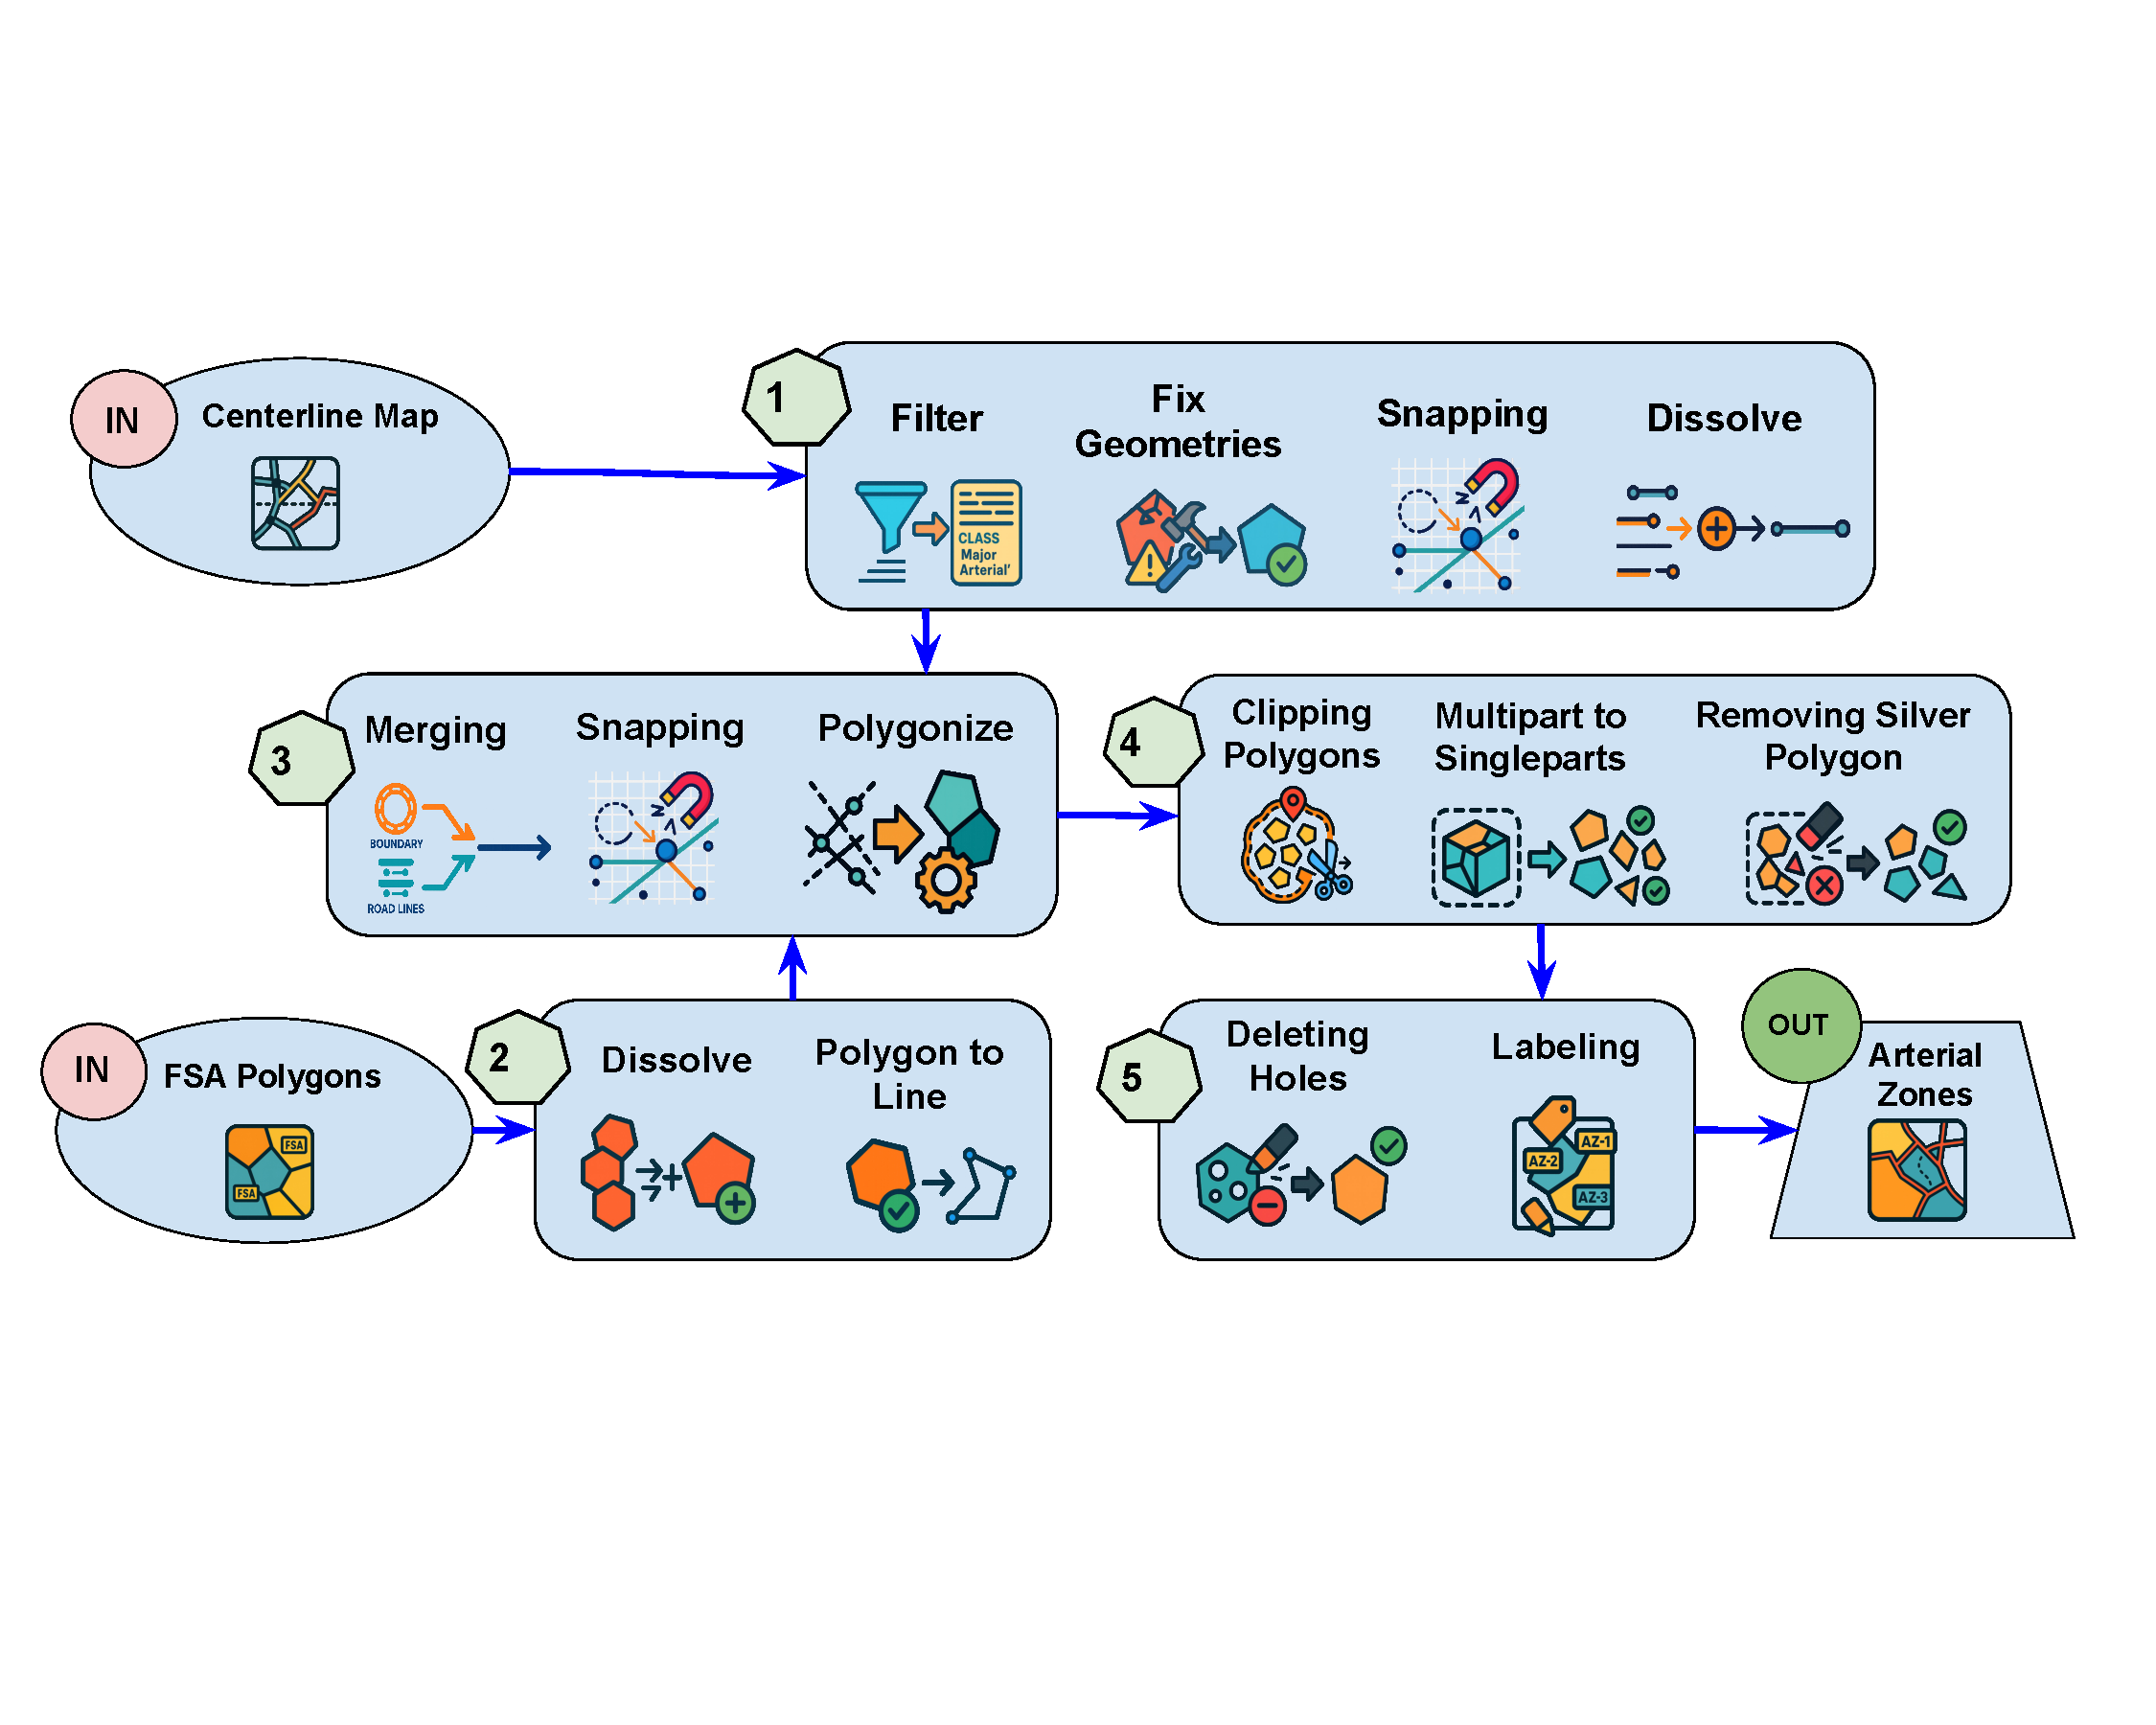
\includegraphics[clip, trim=0.5cm 9.25cm 0.5cm 5.5cm, width=0.9\textwidth]{images/arterial_zoning.pdf}
\caption{Workflow of the arterial zoning algorithm. Road centrelines and \gls{fsa} polygons are processed to produce a set of finalized arterial zones, \gls{ZAr}.}
\label{fig:arterial_zoning_pipeline}
\end{figure}


% \begin{enumerate}
%   \item \textbf{Filter the centreline to major arterials.}
%     \begin{itemize}
%       \item \emph{Layer} $\rightarrow$ \emph{Filter} (or Field Calculator / Select by Expression) with your schema, e.g.:
%       \[
%         \texttt{"CLASS" IN ('Major Arterial','Minor Arterial')}
%       \]
%       (Use your exact field names; definitions align with Table~\ref{tab:road_classes}.)
%       \item \emph{Vector} $\rightarrow$ \emph{Geometry} $\rightarrow$ \textbf{Fix geometries}.
%       \item \emph{Vector} $\rightarrow$ \emph{Geometry} $\rightarrow$ \textbf{Snap geometries} (tolerance \(\sim\) 0.5–1.0~m; to itself) to close micro-gaps that block polygonization.
%       \item \emph{Vector} $\rightarrow$ \emph{Geoprocessing} $\rightarrow$ \textbf{Dissolve} (no dissolve field) to produce a single multiline arterial network (optional but helps polygonization).
%     \end{itemize}

%   \item \textbf{Build the urban boundary from FSAs.}
%     \begin{itemize}
%       \item \emph{Vector} $\rightarrow$ \emph{Geoprocessing} $\rightarrow$ \textbf{Dissolve} on FSA polygons (no field) to create a single \emph{urban boundary} polygon.
%       \item \emph{Vector} $\rightarrow$ \emph{Geometry} $\rightarrow$ \textbf{Polygon to lines} to convert the urban boundary to a line layer (\(\partial\Omega\)).
%     \end{itemize}

%   \item \textbf{Create a planar subdivision bounded by arterials and the urban limit.}
%     \begin{itemize}
%       \item Merge the \emph{arterial lines} with the \emph{boundary lines}:
%         \emph{Processing Toolbox} $\rightarrow$ \textbf{Merge Vector Layers} (or \textbf{Append}).
%       \item Snap again (\emph{Snap geometries}) using the merged layer as both source and target (same 0.5–1.0~m tolerance).
%       \item \emph{Vector} $\rightarrow$ \emph{Geometry} $\rightarrow$ \textbf{Polygonize}. 
%       \item Result: raw faces of the arrangement \( \mathcal{A} = E_{\text{arterial}} \cup \partial\Omega \).
%     \end{itemize}

%   \item \textbf{Clip and clean the faces.}
%     \begin{itemize}
%       \item \emph{Vector} $\rightarrow$ \emph{Geoprocessing} $\rightarrow$ \textbf{Clip} (input: polygonized faces; overlay: urban boundary polygon).
%       \item \emph{Vector} $\rightarrow$ \emph{Geometry} $\rightarrow$ \textbf{Multipart to singleparts}.
%       \item Remove slivers: \emph{Select by Expression} 
%       \[
%         \texttt{\$area < 10\,000} 
%       \]
%       (e.g., $<1$\,ha) $\rightarrow$ delete, or use \textbf{Eliminate sliver polygons} (if available).
%       \item \emph{Vector} $\rightarrow$ \emph{Geometry} $\rightarrow$ \textbf{Delete holes} (threshold e.g., $< 2\,000$\,m\(^2\)) to clean micro-voids.
%     \end{itemize}

%   \item \textbf{Label and finalize arterial zones.}
%     \begin{itemize}
%       \item Add fields via Field Calculator: 
%         \texttt{ZONE\_ID} (e.g., \texttt{'AZ\_' || to\_string(@row\_number)}), 
%         \texttt{AREA\_M2 = \$area}, 
%         \texttt{PERIM\_M = \$perimeter}.
%       \item (Optional) Keep only polygons whose boundaries are mostly arterial: compute the fraction of each face’s perimeter coincident with arterial lines (Overlay \(\rightarrow\) \textbf{Line dissolve} on arterials, then \textbf{Line\_intersections}/\textbf{Line\_locate\_along\_geometry}); filter if needed.
%       \item Export the result as \texttt{arterial\_zones.gpkg} (or shapefile).
%     \end{itemize}
% \end{enumerate}

% \paragraph{Parameter notes (practical and strict).}
% \begin{itemize}
%   \item \textbf{Snapping tolerance:} 0.5–1.0 m typically prevents micro-gaps that break polygonization without over-merging nearby vertices.
%   \item \textbf{Sliver threshold:} Set by map scale and use case. For city-scale zones, $10\,000$–$20\,000$ m\(^2\) is a sensible starting point; tune based on QA.
%   \item \textbf{Topology QA:} If polygonize fails or yields holes, revisit \textbf{Fix geometries} and \textbf{Snap geometries}; inspect dangling ends and overlaps.
% \end{itemize}

\subsection{From \gls{fsa}-level \gls{bev} counts to arterial zones' \gls{bev} densities}\label{sec:Ev_density_for AZ}
Data on vehicle ownership for \gls{bev}s are only available at the \gls{fsa} level, which is the primary record of registered vehicles. Ideally, if ownership data were available at multiple administrative levels, the most detailed unit would be preferred, as higher-resolution data allows for a more accurate representation of spatial variations in \gls{bev} ownership. This improves the allocation of resources to arterial zones and aligns better with major mobility patterns.
The \gls{fsa} polygons are used as the base administrative units. However, \glspl{fsa} do not correspond with mobility corridors and thus do not accurately reflect \gls{bev} activity along major arterial roads. Each \gls{fsa} is intersected with the defined arterial zones, allowing the proportional redistribution of \gls{bev} counts from \gls{fsa} zones to mobility-based arterial zones. This process ensures that \gls{bev} activity is accurately represented within the arterial zones, which serve as the fundamental spatial framework for planning \gls{fc} infrastructure.
The set of intersection regions, denoted by \gls{Zcap}, is defined as
\begin{align}
  \mathcal{Z}^{\cap} 
  \;=\; \bigl\{\, Z^{\cap}_{i,j} \;=\; Z^{\mathrm{FSA}}_i \cap Z^{\mathrm{Ar}}_j \;:\; (i,j)\in\mathcal{K} \,\bigr\}
  \;\subset\; \mathcal{P}(\mathbb{R}^2).
  \label{eq:intersections set}
\end{align}
The index set of valid intersections, \gls{K}, is given by
\begin{align}
  \mathcal{K} \;=\; 
  \bigl\{\, (i,j) \in \mathcal{I}\times\mathcal{J} \;:\;
  \mathrm{Area}\bigl(Z^{\mathrm{FSA}}_i \cap Z^{\mathrm{Ar}}_j\bigr) > 0 \,\bigr\}.
\end{align}
Each \gls{Zcapij} corresponds to a non-empty intersection polygon between the $i$-th \gls{fsa} and the $j$-th arterial zone, that is, all regions where $Z^{\mathrm{FSA}}_i \cap Z^{\mathrm{Ar}}_j$ has positive area.

Let \gls{Area} denote the area functional, which assigns a nonnegative area value to any planar region.
For each \gls{fsa} zone and arterial zone, the corresponding areas are expressed as 

\begin{align}
  A^{\mathrm{FSA}}_i &= \mathrm{Area}\!\left(Z^{\mathrm{FSA}}_i\right), \qquad i \in \mathcal{I}, \label{eq:fsa areas} \\
  A^{\mathrm{Ar}}_j  &= \mathrm{Area}\!\left(Z^{\mathrm{Ar}}_j\right), \qquad j \in \mathcal{J}, \label{eq:artertal_zones_area} \\
  A^{\cap}_{i,j}     &= \mathrm{Area}\!\left(Z^{\mathrm{FSA}}_i \cap Z^{\mathrm{Ar}}_j\right), 
  \qquad (i,j) \in \mathcal{K}, \label{eq:intersections area}
\end{align}
where \gls{Acap} denotes the area of each intersection region between them.
The corresponding set of intersection areas, denoted by \gls{Acapset}, is defined as 
\begin{align}
  \mathcal{A}^{\cap}
  \;=\; \bigl\{\, A^{\cap}_{i,j} 
  :\; (i,j)\in\mathcal{K} \,\bigr\}
  \;\subset\; \mathbb{R}_{\ge 0}.
\end{align}
% Each FSA polygon is then intersected with the arterial regions obtained in the previous step. 
% This ensures that EV counts are spatially redistributed according to the overlap between FSAs and arterial regions. 
% Based on these intersections, the share of EVs belonging to each FSA is allocated to the intersected regions by weighting the EV count of the FSA according to the relative area, i.e.,
The \gls{fsa}-level \gls{bev} counts are redistributed to the intersection regions~\eqref{eq:intersections set} in proportion to their relative areas, as specified by~\eqref{eq:fsa areas} and~\eqref{eq:intersections area}, with the allocation given in~\eqref{eq:EV_allocation_intersection}:
\begin{align}  \label{eq:EV_allocation_intersection}
    \mathrm{EVC}_{i \cap j} \;=\;
    \frac{A^{\cap}_{i,j}}{A^{\mathrm{FSA}}_i} \,\times\, EVC_i,
    \qquad (i,j) \in \mathcal{K},
\end{align}
Here, \gls{EVCcap} denotes the portion of the \gls{bev} count from \gls{fsa}~$i$ that is allocated to the intersection region \gls{Zcapij}.
The set of \gls{bev} counts allocated to intersection regions, denoted by \gls{EVCcapset}, is defined as
\begin{equation} 
\label{eq:ev_counts_for_intersection}
  \mathcal{E}^{\cap}
  \;=\; \bigl\{\, \mathrm{EVC}_{i \cap j} 
  : (i,j)\in\mathcal{K} \,\bigr\}
  \;\subset\; \mathbb{R}_{\ge 0},
\end{equation}
% where each element $\mathrm{EVC}_{i \cap j}$ is given by~\eqref{eq:EV_allocation_intersection} and represents 
% the share of \gls{bev}s from FSA~$i$ assigned to the intersection region $Z^{\cap}_{i,j}$.
The aggregate \gls{bev} count for each arterial region, denoted by \gls{EVCAr}, is obtained by summing the allocated intersection shares over all \glspl{fsa} that intersect the $j$-th arterial zone (\gls{ZArj}), defined as
\begin{equation}
  \label{eq:EV_aggregate_arterial}
  \mathrm{EVC}^{\mathrm{Ar}}_{j}
  \;=\;
  \sum_{i:\,(i,j)\in\mathcal{K}} \mathrm{EVC}_{i \cap j},
  \qquad j \in \mathcal{J}.
\end{equation}
Aggregation of the arterial-level \gls{bev} counts yields the set \gls{EVCArset}, defined as
\begin{equation}
  \mathcal{E}^{\mathrm{Ar}}
  \;=\;
  \bigl\{\, \mathrm{EVC}^{\mathrm{Ar}}_{j} : j \in \mathcal{J} \,\bigr\}
  \;\subset\; \mathbb{R}_{\ge 0}.
\end{equation}
To standardize across zones of varying size, the \gls{bev} density for each arterial zone, denoted by \gls{rhoAr}, is defined as
\begin{align}
  \label{eq:EV_density_arterial}
  \rho^{\mathrm{Ar}}_{j}
  \;=\;
  \frac{\mathrm{EVC}^{\mathrm{Ar}}_{j}}{A^{\mathrm{Ar}}_{j}},
  \qquad j \in \mathcal{J}, \; A^{\mathrm{Ar}}_{j}>0.
\end{align}
For comparability across regions, the \gls{bev} densities are rescaled to the unit interval through min–max normalization. The normalized density for each arterial region, denoted by \gls{rhoArHat}, is defined as
\begin{align}
  \label{eq:EV_density_norm}
  \widehat{\rho}^{\mathrm{Ar}}_{j}
   \;=\;
   \frac{\rho^{\mathrm{Ar}}_{j} - \min_{k \in \mathcal{J}} \rho^{\mathrm{Ar}}_{k}}
        {\max_{k \in \mathcal{J}} \rho^{\mathrm{Ar}}_{k} - \min_{k \in \mathcal{J}} \rho^{\mathrm{Ar}}_{k}},
   \qquad j \in \mathcal{J},
\end{align}
which ensures $\widehat{\rho}^{\mathrm{Ar}}_{j} \in [0,1]$ for all $j$. The set of normalized \gls{bev} densities for all arterial zones, denoted by \gls{rhoArNormSet}, is defined as
\begin{align}
  \label{eq:EV_density_norm_set}
  \widehat{\mathcal{R}}^{\mathrm{Ar}}
   \;=\;
   \bigl\{\, 
      \widehat{\rho}^{\mathrm{Ar}}_{j} 
      : j \in \mathcal{J} 
   \,\bigr\}.
\end{align}
\subsection{Graph construction and hop distance}
\label{subsec:hop_distance}
To represent spatial connectivity among arterial zones, an undirected planar adjacency graph \gls{GraphG} is constructed.
Each arterial zone \gls{ZArj} corresponds to a vertex \gls{VertexVj}, whose position is defined by the geometric centroid functional \gls{Centroid}.
The graph is defined as
\begin{align}
G=(V,E,W),\qquad 
V=\{\,v_j : j\in\mathcal{J}\,\},\;\; v_j \leftrightarrow \mathrm{Centroid}(Z^{\mathrm{Ar}}_j),\label{eq:urban_graph}
\end{align}
where \gls{VertexSet} denotes the set of vertices, \gls{EdgeSet} represents the set of undirected edges, and \gls{WeightMatrix} contains the edge weights.
Two arterial zones are considered adjacent if they share a boundary of positive length.
Let \gls{Boundary} denote the boundary operator and \gls{Length} the boundary-length functional, both computed under the working projection defined in \ref{def:projection}.
The binary adjacency matrix \gls{AdjacencyMatrix} represents the topological connectivity between arterial zones.
Each element \gls{AdjacencyAjk} indicates whether two zones share a common boundary of positive length, defined as

\begin{align}
\label{eq:adjacency_unweighted_fixed}
A_{jk}
=\begin{cases}
1, & \mathrm{Length}\!\bigl(\partial Z^{\mathrm{Ar}}_j \cap \partial Z^{\mathrm{Ar}}_k\bigr) > 0,\ j\neq k,\\[0.25em]
0, & \text{otherwise},
\end{cases}
\qquad j,k \in \mathcal{J},\quad A_{jj}=0.
\end{align}
The weighted adjacency matrix \gls{WeightMatrix} encodes the geometric strength of connections between arterial zones.
Each element \gls{WeightedElement} represents the length of the shared boundary between the two arterial zones \gls{ZArj} and $Z^{\mathrm{Ar}}_k$, defined as
\begin{align}
\label{eq:adjacency_weight_fixed}
w_{jk}
=\mathrm{Length}\!\bigl(\partial Z^{\mathrm{Ar}}_j \cap \partial Z^{\mathrm{Ar}}_k\bigr),
\qquad j,k \in \mathcal{J},\quad w_{jk}=w_{kj}\ge 0,\quad w_{jj}=0.
\end{align}

The hop distance \gls{HopDistance} measures the topological separation between two arterial zones in the unweighted adjacency graph.
It is defined as the number of edges in the shortest path between vertices \gls{VertexVj} and $v_k$ in the graph \gls{GraphG} is defined as
\begin{align}
\label{eq:hop_distance}
d_G(j,k)
=\min_{\pi:j\rightsquigarrow k}\; |\pi|,
\end{align}
where \gls{PathPi} denotes a path connecting \gls{VertexVj} and $v_k$ in $G$, and $|\pi|$ is the number of edges in that path. 
If no connecting path exists, $d_G(j,k)=\infty$. 
The one-hop neighbor set \gls{NeighborSet} and its $h$-hop generalization \gls{NeighborSetH} are defined as
\begin{align}
\label{eq:direct_neibours}
N(j)        &= \{\, k\in\mathcal{J} : A_{jk}=1 \,\}, \\
\label{eq:hop_rings}
N^{(h)}(j)  &= \{\, k\in\mathcal{J} : d_G(j,k)=h \,\}, \quad h=0,1,2,\dots
\end{align}
% and the closed $n$-hop ball used in smoothing, as defined in~\eqref{eq:EV_density_nhop_ball}, is

% \begin{equation}
% \label{eq:hop_ball}
% B^{(n)}(j)=\{\, k\in\mathcal{J} : d_G(j,k)\le n \,\}.
% \end{equation}

% \paragraph{Practical notes.}
% (i) Use an equal-area or metrically appropriate projection so that $\mathrm{Length}(\cdot)$ reflects true shared-boundary distances. 
% (ii) Hop distance is combinatorial and ignores $w_{jk}$ by design (weights can be incorporated later via ring weights or stochastic averaging). 
% (iii) Smoothing and aggregation are applied within the connected component containing $j$; if $d_G(j,k)=\infty$, then $k\notin B^{(n)}(j)$ for any finite $n$.


\subsection{Weighted $n$-hop smoothing}
\label{subsec:nhop_smoothing}
% Spatial smoothing replaces each arterial-zone EV density with a local average over its neighbors on the adjacency graph, reflecting spillovers and reducing small-area noise. Concretely, starting from the unsmoothed densities $\rho^{\mathrm{Ar}}_{j}$ in~\eqref{eq:EV_density_arterial}, we compute a smoothed value by averaging over neighboring zones using the weighted $n$-hop ball in~\eqref{eq:EV_density_nhop_weighted}. We smooth for two reasons: (i) EV ownership and charging demand exhibit spatial dependence along corridors and across adjacent neighborhoods, which a local average captures; and (ii) raw densities can be unstable in small or sparsely connected zones, so smoothing borrows strength from neighbors. The hyperparameter $n$ and ring weights control the spatial scale of influence, trading variance reduction against potential over-smoothing.
% Given the arterial zones' EV densities $\rho^{\mathrm{Ar}}_{k}$ from~\eqref{eq:EV_density_arterial}, the $n$-hop distance-sensitive smoothing, uses ring weights over hop shells is \begin{align}
%   \label{eq:EV_density_nhop_weighted}
%   \tilde{\rho}^{\mathrm{Ar}}_{j}(n,\mathbf{w})
%   \;=\;
%   \sum_{h=0}^{n} 
%   w_h \;\frac{1}{\lvert N^{(h)}(j)\rvert}
%   \sum_{k \in N^{(h)}(j)} \rho^{\mathrm{Ar}}_{k},
%   \qquad j \in \mathcal{J},
% \end{align}
%  $N^{(h)}(j)$ is h-hop neibour zones from Equation~\eqref{eq:hop_rings} and choose nonnegative weights 
% $\mathbf{w}=(w_0,\dots,w_n)$ with $\sum_{h=0}^{n} w_h=1$. 

% with the convention that empty rings $N^{(h)}(j)=\varnothing$ are omitted and the remaining
% weights are renormalized.

% \noindent Equation~\eqref{eq:EV_density_nhop_weighted} defines an $n$-hop ring-weighted smoother. 
% For each arterial zone $j$, the set $N^{(h)}(j)=\{\,k\in\mathcal{J}: d_G(j,k)=h\,\}$ collects the zones at $h$ hops from $j$ in the adjacency graph, with $N^{(0)}(j)=\{j\}$. 
% The vector $\mathbf{w}=(w_0,\dots,w_n)$ contains nonnegative ring weights that sum to one, $\sum_{h=0}^{n} w_h=1$, and controls how influence decays with hop distance. 
% Within each ring $N^{(h)}(j)$, the formula first takes the simple average of the unsmoothed densities $\rho^{\mathrm{Ar}}_k$, the inner sum divided by $|N^{(h)}(j)|$, the number of neighborhood zones plus one, and then forms a convex combination of these ring averages across $h=0,\dots,n$ using the weights $w_h$.

% \noindent If $n=0$, then $\tilde{\rho}^{\mathrm{Ar}}_{j}(0,\mathbf{w})=\rho^{\mathrm{Ar}}_{j}$ (no smoothing). If $w_0=\cdots=w_n=\tfrac{1}{n+1}$, uniform ring weights, and every ring is nonempty, the result is the mean of the ring-wise means. If one chooses $w_h \propto |N^{(h)}(j)|$ and renormalizes over $h$ so weights depend on $j$. Empty rings are omitted in practice; when some $N^{(h)}(j)=\varnothing$, the remaining $w_h$ are renormalized to sum to one.
% The operator is a convex average that preserves units (e.g., vehicles/km$^2$) and lies between the minimum and maximum densities observed within the $n$-hop neighborhood. 
% Choosing $\mathbf{w}$ (e.g., geometric decay $w_h \propto \lambda^h$ with $\lambda\in(0,1)$) tunes the spatial scale of influence: larger mass on small $h$ preserves local detail; heavier tails in $h$ emphasize broader corridor- or region-level spillovers.
Spatial smoothing replaces each arterial-zone \gls{bev} density with a locally averaged value over its neighbouring zones in the adjacency graph \gls{GraphG}, thereby capturing spatial spillover effects and reducing small-area variability. 
Starting from the unsmoothed normalized densities \gls{rhoArHat}, the smoothed density for zone $j$, denoted by \gls{rhoArSmooth}, is defined as

\begin{align}
  \label{eq:EV_density_nhop_weighted}
  \tilde{\rho}^{\mathrm{Ar}}_{j}(n,\mathbf{w})
  \;=\;
  \sum_{h=0}^{n} 
  w_h \;\frac{1}{\lvert N^{(h)}(j)\rvert}
  \sum_{k \in N^{(h)}(j)} \widehat{\rho}^{\mathrm{Ar}}_{k},
  \qquad j \in \mathcal{J},
\end{align}
where \gls{NeighborSetH} denotes the $h$-hop neighbour set defined in~\eqref{eq:hop_rings}, $N^{(0)}(j)=\{j\}$, and \gls{WeightVector} is the vector of nonnegative hop weights satisfying $\sum_{h=0}^{n} w_h=1$. 
Neighbour sets with $\lvert N^{(h)}(j)\rvert=0$ are excluded from the computation, and the remaining weights are renormalized accordingly. 
The set of smoothed \gls{bev} densities across all arterial zones, denoted by \gls{rhoArSmoothSet}, is defined as  

\begin{align}
  \label{eq:EV_density_set}
  \widetilde{\mathcal{D}}^{\mathrm{Ar}}(n,\mathbf{w})
   \;=\;
   \bigl\{\, 
      \tilde{\rho}^{\mathrm{Ar}}_{j}(n,\mathbf{w}) 
      : j \in \mathcal{J} 
   \,\bigr\},
\end{align}
which enumerates the smoothed densities \gls{rhoArSmooth}$(n,\mathbf{w})$ 
in~\eqref{eq:EV_density_nhop_weighted} for all arterial zones 
$j \in $ \gls{J}.
Equation~\eqref{eq:EV_density_nhop_weighted} defines an \gls{nHop}-hop weighted smoothing of \gls{bev} densities. The operation proceeds in two steps. First, for each hop distance $h$, the densities of the $h$-hop neighbours of a given zone are averaged uniformly over the corresponding neighbour set. This produces a mean value that reflects the influence of all zones exactly $h$ steps away. Second, these ring-wise averages are combined across hop levels using a convex weight vector \gls{WeightVector}. The result is a weighted mixture of contributions from multiple spatial scales, with $\mathbf{w}$ controlling the relative importance of nearer versus farther neighbours.
 % This construction maintains the original density units (e.g., vehicles/km²). If we set \( n=0 \), we obtain \( \tilde{\rho}^{\mathrm{Ar}}_{j}=\widehat{\rho}^{\mathrm{Ar}}_{j} \), which indicates no smoothing. 
 % Uniform hop weights $w_h=\tfrac{1}{n+1}$, when all neighbour sets are nonempty, produce the mean of the hop-wise means. Choosing $w_h \propto \lvert N^{(h)}(j)\rvert$ and renormalizing over $h$ collapses to the unweighted $n$-hop ball average in~\eqref{eq:EV_density_nhop_ball}. 
The hyperparameters $n$ and $\mathbf{w}$ control the spatial scale of influence, trading variance reduction against potential over-smoothing. A geometric decay scheme, $w_h \propto \lambda^h$ with $\lambda \in (0,1)$, emphasizes local structure while still allowing broader spillover effects.

% The outputs of this stage are visualized through heatmaps of both the raw density $\rho_i$ and the smoothed density $\tilde{\rho}_i$, which reveal spatial variation and hotspots across the arterial zoning system (Figure~\ref{fig:ev_density_heatmap}).

% \begin{figure}[htbp]
% \centering
% \includegraphics[width=0.85\textwidth]{images/EV_density_heatmap.pdf}
% \caption{Heatmap of EV density across arterial regions based on proportional allocation of FSA-level counts.}
% \label{fig:ev_density_heatmap}
% \end{figure}

% \begin{figure}[htbp]
% \centering
% \includegraphics[width=0.75\textwidth]{images/Arteril_EV_Density_heatmap.pdf}
% \caption{Smoothed EV density heatmap using one-hop adjacency diffusion, highlighting density gradients and regional hotspots.}
% \label{fig:smoothed_ev_density_heatmap}
% \end{figure}

\subsection{Ridge paths as \gls{bev} activity backbones}\label{sec:Ridge paths}
Ridge paths are introduced as structural backbones of \gls{bev} activity and charging-demand proxies.
They are extracted from the smoothed \gls{bev} density surface across the city's arterial zones, highlighting the most prominent spines of \gls{bev} movement and concentration.
 Conceptually, they represent concentrated movement patterns and strategic urban corridor zones where charging demand is expected to be greatest. Unlike uniform thresholding methods, ridge paths adapt to the relative peaks in the density field and align with the directional flow of activity. Therefore, they offer a spatially-aware, activity-driven basis for positioning \gls{fc} infrastructure along significant, high-usage urban routes. Ridge paths are defined as sequences of connected areas characterized by a decreasing yet consistently high \gls{bev} density. These paths are formed by tracing downward from local maxima on the density surface, allowing the density to decrease gradually based on a controlled drop ratio. This regulation ensures that small local dips do not prematurely interrupt the paths, thereby maintaining continuity along important high-activity corridor zones. Each resulting ridge path effectively captures a coherent high-flow activity line, acting as a proxy for zones where latent charging corridors exist within the urban.

\subsubsection{Ridge path extraction}
The set of local maxima, denoted by \gls{M}, consists of all arterial zones in \gls{J} whose smoothed densities \gls{rhoAr} are not smaller than those of any neighboring zones \gls{NeighborSet}. Each element of \gls{M} represents an arterial zone that attains a locally dominant demand level within its adjacency neighborhood, thereby serving as a potential origin point for ridge-path extraction in the density field:
\begin{equation}
  \label{eq:local_maxima_set}
  \mathcal{M}
   \;=\;
   \bigl\{\, 
      j \in \mathcal{J} 
      : \tilde{\rho}^{\mathrm{Ar}}_{j}(n,\mathbf{w}) 
        \ge \tilde{\rho}^{\mathrm{Ar}}_{i}(n,\mathbf{w}),\;
        \forall i \in N(j)
   \,\bigr\},
\end{equation}
where \gls{NeighborSet} denotes the set of direct neighbors of arterial zone~$j$ as defined in~\eqref{eq:direct_neibours}.

For each local maximum $v_m \in \mathcal{M} \subseteq V$, where \gls{VertexSet} denotes the the set of nodes in the urban graph, a ridge path, denoted by \gls{rp_m}, is defined as a finite sequence of nodes 
\begin{align}
  \label{eq:ridge_path}
  \mathsf{rp_m} \;=\; (v_m, \dots, v_k, \dots, v_\ell),
\end{align}
such that $v_m \in \mathcal{M}$ is a local maximum from~\eqref{eq:local_maxima_set},
$(v_{k}, v_{k+1}) \in E$ for all $k = m, \dots, \ell$, where \gls{EdgeSet} denotes the the set of edges in the urban graph, and the sequence satisfies the density-drop condition
\begin{align}
   \tilde{\rho}^{\mathrm{Ar}}_{v_{k+1}}(n,\mathbf{w}) 
   \;\ge\; \tilde{\rho}^{\mathrm{Ar}}_{v_{k}}(n,\mathbf{w}) - \Delta,
   \qquad k = m, \dots, \ell,
\end{align}
for a chosen drop tolerance $\Delta > 0$. The parameter \gls{Delta} controls the maximum allowable decline in smoothed \gls{bev} density between consecutive nodes. The set of all ridge paths originating from local maxima constitutes the ridge-path set, denoted by \gls{RP}, and is defined as
\begin{align}
  \label{eq:ridge_path_set}
  \mathcal{RP}
   = \bigl\{\,
      \mathsf{rp_m} = (v_m, \dots, v_\ell)
      \;\big|\;
      v_m \in \mathcal{M},\;
      (v_k, v_{k+1}) \in E
   \,\bigr\}.
\end{align}

A ridge path is constructed by iteratively traversing neighboring zones whose smoothed density remains within a strategy-specific drop tolerance. At iteration $t$ with current node $v_t$, let the feasible neighbor set be defined as
\begin{align}
N_t &= N(v_t)\setminus \{v_m,\dots,v_t\}, 
&
\mathcal{D}_t &= \{\tilde{\rho}^{\mathrm{Ar}}_u : u \in N_t\},
\end{align}
where $N(v_t)$ denotes the adjacency set of $v_t$ in \gls{VertexSet}.
\gls{Nt} collects all unvisited neighbors of the current node $v_t$, 
while \gls{Dt} records the corresponding smoothed density values. 
At each step, the ridge-walking algorithm selects the next node $v_{t+1}$ from 
$N_t$ according to a density-based rule,
\begin{align}
v_{t+1} \;=\; \arg\max_{u \in N_t} \tilde{\rho}^{\mathrm{Ar}}_u
\quad \text{subject to } 
\tilde{\rho}^{\mathrm{Ar}}_u \ge \tilde{\rho}^{\mathrm{Ar}}_{v_t} - \Delta_t,
\end{align}
% where $\Delta_t>0$ is the drop tolerance at step $t$. The statistic $S_t$ and drop allowance \gls{Deltat} depend on the chosen
% strategy $m \in \{\textsc{avg}, \textsc{max}, \textsc{median}, 
% \textsc{std}, \textsc{laplacian}\}$:
The drop allowance \gls{Deltat} is determined according to the selected ridge-walking strategy, denoted by \gls{St}, average, maximum, median, standard deviation, or Laplacian, which defines how local density information is aggregated into an adaptive tolerance threshold  as follows:

\begin{align}
\label{eq:ridge_avg}
\textsc{avg:}       && S_t &= \operatorname{mean}(\mathcal{D}_t),            
& \Delta_t &= \tfrac{\eta}{2}\!\left(\tilde{\rho}^{\mathrm{Ar}}_{v_t}+S_t\right), \\[4pt]
\label{eq:ridge_max}
\textsc{max:}       && S_t &= \max(\mathcal{D}_t),                            
& \Delta_t &= \tfrac{\eta}{2}\!\left(\tilde{\rho}^{\mathrm{Ar}}_{v_t}+S_t\right), \\[4pt]
\label{eq:ridge_median}
\textsc{median:}    && S_t &= \operatorname{median}(\mathcal{D}_t),           
& \Delta_t &= \tfrac{\eta}{2}\!\left(\tilde{\rho}^{\mathrm{Ar}}_{v_t}+S_t\right), \\[4pt]
\label{eq:ridge_std}
\textsc{std:}       && S_t &= \operatorname{std}(\mathcal{D}_t),              
& \Delta_t &= \eta\,S_t, \\[4pt]
\label{eq:ridge_laplacian}
\textsc{laplacian:} && S_t &= \tilde{\rho}^{\mathrm{Ar}}_{v_t}-\operatorname{mean}(\mathcal{D}_t), 
& \Delta_t &= \eta\,S_t.
\end{align}

% $\eta$ is a scaling hyperparameter that calibrates the threshold $\Delta_t$ across different strategies, thereby controlling the ridge-walker's balance between strictness and flexibility.
The scaling hyperparameter \gls{eta} calibrates the threshold \gls{Deltat} across different strategies, thereby controlling the ridge-walker's balance between strictness and flexibility.
The candidate set of admissible neighbors, denoted by \gls{Ct}, is defined as

\begin{equation}
\mathcal{C}_t = 
\{\,u \in N_t : 
   \tilde{\rho}^{\mathrm{Ar}}_{u} \ge \tilde{\rho}^{\mathrm{Ar}}_{v_t} - \Delta_t \,\}.
\end{equation}
If $\mathcal{C}_t = \varnothing$, the walk terminates. Otherwise, we set
\begin{equation}
v_{t+1} \in \arg\max_{u \in \mathcal{C}_t}\tilde{\rho}^{\mathrm{Ar}}_{u},
\end{equation}
append $v_{t+1}$ to the path, and continue until reaching the maximum 
walk length \gls{L} or termination. To limit the extent of such paths, A maximum walk length, denoted as \gls{L}, is established to control the extent to which a ridge path can extend within the graph.
This constraint prevents excessively long ridge paths that could lose clarity and interpretability as concentrated activity corridor zones.
To maintain consistency with the network structure, \gls{L} is bounded above by the diameter of the graph:
\begin{align}
\operatorname{diam}(G) = \max_{u,v \in V} d_G(u,v),
\end{align}
where \gls{dGuv} represents the hop distance, defined as the length of the shortest path between nodes $u$ and $v$ in the graph.
Given that no ridge path can exceed this limit, we require
\begin{align}
    L &\;\leq\; \operatorname{diam}(G).
\end{align}
To localize ridge-path extraction and prevent unrealistically long trajectories, the maximum walk length \gls{L} is defined as a fraction of the graph diameter \gls{diamG}, scaled by the proportionality factor \gls{alpha}:
\begin{align}
    L &= \alpha \cdot \operatorname{diam}(G),
    \qquad \alpha \in (0,1].
\end{align}
Here, \gls{alpha} controls the relative extent of ridge paths with respect to the overall network size.
Beyond the maximum walk length, ridge-path construction is further constrained by a density-based stopping criterion. Specifically, the walk continues until the average smoothed density along the traversed ridge falls below a prescribed threshold \gls{rhoMin}, defined as the 75th percentile of the \gls{bev} density distribution across all arterial zones. A candidate ridge path \gls{rp_m} is retained only if its mean density satisfies
\begin{align}
\frac{1}{\ell+1}\sum_{i=m}^{\ell+m} \tilde{\rho}^{\mathrm{Ar}}_{v_i} 
\;\geq\; \bar{\rho}_{\min}.
\end{align}


% \subsubsection*{Ridge Extraction: Strategy Family and Hyperparameterized Pipeline}

% Let $G=(V,E)$ be the arterial adjacency graph, and let $\rho^{\mathrm{Ar}}_v$ denote the (raw or smoothed) EV density at node $v\in V$. For a starting peak $s\in V$, a \emph{ridge walker} constructs a path 
% \(
% \mathsf{path}=(v_0,v_1,\dots,v_\ell)
% \)
% with $v_0=s$ by iteratively moving to a neighbor that maintains a bounded drop relative to the current node under a strategy-specific tolerance. We use two global hyperparameters: the maximum walk length $L\in\mathbb{N}$ and the drop tolerance parameter $\eta>0$. After path construction, paths are retained only if their average density exceeds a screening threshold $\bar{\rho}_{\min}$.

% \paragraph{Strategy-specific drop rules.}
% At step $t$, with current node $v_t$ and neighbor set $N(v_t)$, let the neighbor densities be 
% \(
% \mathcal{D}_t=\{\rho^{\mathrm{Ar}}_u: u\in N(v_t)\}.
% \)
% Define a strategy statistic $S_t$ on $\mathcal{D}_t$ and a drop allowance $\Delta_t$ as follows:
% \begin{align*}
% \textsc{avg:}       && S_t &= \operatorname{mean}(\mathcal{D}_t),            & \Delta_t &= \tfrac{\eta}{2}\!\left(\rho^{\mathrm{Ar}}_{v_t}+S_t\right),\\
% \textsc{max:}       && S_t &= \max(\mathcal{D}_t),                            & \Delta_t &= \tfrac{\eta}{2}\!\left(\rho^{\mathrm{Ar}}_{v_t}+S_t\right),\\
% \textsc{median:}    && S_t &= \operatorname{median}(\mathcal{D}_t),           & \Delta_t &= \tfrac{\eta}{2}\!\left(\rho^{\mathrm{Ar}}_{v_t}+S_t\right),\\
% \textsc{std:}       && S_t &= \operatorname{std}(\mathcal{D}_t),              & \Delta_t &= \eta\,S_t,\\
% \textsc{laplacian:} && S_t &= \rho^{\mathrm{Ar}}_{v_t}-\operatorname{mean}(\mathcal{D}_t), \quad & \Delta_t &= \eta\,S_t.
% \end{align*}
% The next node is chosen from the candidate set
% \[
% \mathcal{C}_t \;=\; \left\{\, u\in N(v_t)\setminus \{v_0,\dots,v_t\} \;:\; \rho^{\mathrm{Ar}}_{u} \ge \rho^{\mathrm{Ar}}_{v_t}-\Delta_t \,\right\},
% \]
% by taking the highest-density admissible neighbor:
% \(
% v_{t+1} \in \arg\max_{u\in \mathcal{C}_t}\rho^{\mathrm{Ar}}_u.
% \)
% The walk stops if $\mathcal{C}_t=\varnothing$ or when $t=L-1$.

% \begin{algorithm}[H]
% \caption{Hyperparameterized Ridge Extraction with Strategy Set}
% \label{alg:ridge_extraction}
% \DontPrintSemicolon
% \KwIn{Graph $G=(V,E)$ with densities $\rho^{\mathrm{Ar}}_v$; set of local maxima $\mathcal{P}\subseteq V$; strategy set $\mathcal{M}=\{\textsc{avg},\textsc{max},\textsc{median},\textsc{std},\textsc{laplacian}\}$; max steps $L$; drop parameter $\eta>0$ (or per-strategy $\eta_m$); average-density threshold $\bar{\rho}_{\min}$.}
% \KwOut{Dictionary $\mathsf{StrategyRidges}$ mapping $m\in\mathcal{M}$ to retained ridge paths and annotations.}

% $\mathsf{StrategyRidges}\leftarrow \{\}$\;
% \ForEach{$m\in \mathcal{M}$}{
%   $\mathsf{Ridges}\leftarrow [\,]$, \quad $\mathsf{Annot}\leftarrow [\,]$\;
%   \ForEach{$s\in \mathcal{P}$}{
%     $\mathsf{path}\leftarrow [s]$, \; $\mathsf{visited}\leftarrow \{s\}$, \; $v\leftarrow s$\;
%     \For{$t\leftarrow 0$ \KwTo $L-1$}{
%       $\mathcal{N}\leftarrow N(v)\setminus \mathsf{visited}$\;
%       \If{$\mathcal{N}=\varnothing$}{\textbf{break}}
%       Compute $\mathcal{D}=\{\rho^{\mathrm{Ar}}_u: u\in \mathcal{N}\}$\;
%       Compute $S$ and $\Delta$ according to strategy $m$ \tcp*{see rules above}
%       $\mathcal{C}\leftarrow \{u\in \mathcal{N}: \rho^{\mathrm{Ar}}_u \ge \rho^{\mathrm{Ar}}_{v}-\Delta\}$\;
%       \If{$\mathcal{C}=\varnothing$}{\textbf{break}}
%       $v\leftarrow \arg\max_{u\in \mathcal{C}} \rho^{\mathrm{Ar}}_u$\;
%       append $v$ to $\mathsf{path}$; add $v$ to $\mathsf{visited}$\;
%     }
%     \If{$|\mathsf{path}|\ge 2$}{
%       $\bar{\rho}\leftarrow \frac{1}{|\mathsf{path}|}\sum_{u\in \mathsf{path}}\rho^{\mathrm{Ar}}_u$\;
%       \If{$\bar{\rho}\ge \bar{\rho}_{\min}$}{
%         append $(\mathsf{path},\bar{\rho})$ to $\mathsf{Ridges}$\;
%         $u^\star \leftarrow \mathsf{path}[\lfloor |\mathsf{path}|/2\rfloor]$ \tcp*{mid-node for labeling}
%         append $(u^\star,\bar{\rho})$ to $\mathsf{Annot}$\;
%       }
%     }
%   }
%   $\mathsf{StrategyRidges}[m]\leftarrow \{\texttt{ridges}:\mathsf{Ridges},\;\texttt{annot}:\mathsf{Annot}\}$\;
% }
% \Return $\mathsf{StrategyRidges}$\;
% \end{algorithm}
% \noindent\textit{Notes.} (i) $\eta$ acts as a \emph{drop threshold}: larger $\eta$ yields more permissive walks (longer ridges), while smaller $\eta$ enforces stricter descent control. For \textsc{std} and \textsc{laplacian}, $\eta$ functions as a scale multiplier. (ii) The screening threshold $\bar{\rho}_{\min}$ filters out weak or noisy ridges. (iii) The per-strategy $\eta_m$ can be used if different tolerances are desired across $\mathcal{M}$.
% 
% If this condition is violated, the ridge walk terminates. 
This criterion serves as a hyperparameter of the walker algorithm, ensuring that extracted ridge paths remain concentrated within high-activity corridor zones and do not diffuse into sparsely populated regions.
The set of all nodes participating in ridge paths, denoted by \gls{VRP}, is defined as the union of nodes across all ridge paths specified in~\eqref{eq:ridge_path_set}:
\begin{align}
\label{eq:ridge_path_nodes}
\mathcal{V}_{\mathrm{RP}}
\;=\;
\bigcup_{\mathsf{rp_m}\in\mathcal{RP}}
\{\, v_m, \dots, v_\ell \,\}.
\end{align}
Each element of \gls{VRP} represents a centroid of an arterial zone that rests along at least one extracted ridge path, together outlining the spatial footprint of the mobility-based activity structure within the urban graph.

% A ridge-path extraction method is applied to identify EV activity corridors without
% reliance on rasterized demand surfaces. Multi-strategy walkers (average, maximum,
% Laplacian) are employed to trace density ridges from EV ownership distributions. These
% ridge paths are then snapped to the arterial road network, producing demand corridors
% that align both with intensity of EV activity and with underlying mobility structure.

\subsection{Graph-based proximity evaluation}
Corridor zones are represented as nodes positioned along ridge paths, with each node characterized by specific attributes, such as \gls{bev} density acting as a demand proxy and charger density functioning as a supply proxy. Proximity metrics are calculated between ridge-path nodes and charger nodes, using hop-distance measures that are weighted by \gls{bev} density, along with inverse-distance accessibility indices. The effectiveness of this spatial configuration is assessed by comparing it to randomized baseline scenarios, where charger locations are shuffled to create null models for evaluation.

\subsubsection{Charger capacity density as supply proxy}
The supply of charging infrastructure is represented by the aggregate charging capacity assigned to each arterial zone. Let \gls{C} denote the set of charger stations deployed within the study area. Each charger \gls{c} $ \in $ \gls{C} is characterized by a geographic location $\mathrm{loc}(c) \in \mathbb{R}^2$ and a rated capacity $P_c \in \mathbb{R}_{>0}$. Chargers are spatially assigned to arterial zones through the mapping
\begin{align}
  \label{eq:charger_mapping}
  \phi : \mathcal{C} \;\longrightarrow\; \mathcal{J}, 
  \qquad \phi(c) = j \;\;\text{if}\;\; \mathrm{loc}(c) \in Z^{\mathrm{Ar}}_j,
\end{align}
where \gls{J} denotes the index set of arterial zones and 
$Z^{\mathrm{Ar}}_j \subset \mathbb{R}^2$ represents the polygonal footprint of arterial zone $j$. 
Accordingly, each charger \gls{c} is uniquely mapped to the arterial zone that spatially contains it.
% Each charger $c$ is associated with a rated capacity $P_c$. 
% The total charging capacity for zone $j$ is then defined as
% \begin{align}
% \mathrm{Cap}^{\mathrm{Ar}}_{j} 
%    &= \sum_{\substack{c \in \mathcal{C}\\ c \in Z^{\mathrm{Ar}}_j}} P_c .
% \end{align}
% Each charger $c$ is associated with a rated capacity $P_c \in \mathbb{R}_{>0}$.
The subset of chargers located within arterial zone $j$, denoted by \gls{Cj}, is defined as
\begin{align}
  \label{eq:chargers_in_zone}
  \mathcal{C}_j \;=\; \{\, c \in \mathcal{C} \;:\; \mathrm{loc}(c) \in Z^{\mathrm{Ar}}_j \,\}.
\end{align}
% Each element of \gls{Cj} corresponds to an individual charger \gls{c} whose geographic position lies within the spatial boundary of arterial zone $j$.
The total charging capacity assigned to arterial zone $j$, denoted by \gls{CapArj}, is computed as
\begin{align}
  \label{eq:Cap_zone_by_subset}
  \mathrm{Cap}^{\mathrm{Ar}}_{j}
  \;=\;
  \sum_{c \in \mathcal{C}_j} P_c,
  \qquad j \in \mathcal{J}.
\end{align}
% Here, $\mathrm{Cap}^{\mathrm{Ar}}_{j}$ represents the aggregate rated power of all chargers located within zone $j$, providing a quantitative measure of local charging supply.
To standardize across regions of varying size, the charger capacity density for each arterial zone, denoted by \gls{rhoChj}, is defined as
\begin{align}
  \label{eq:Charger_capacity_density}
  \rho^{\mathrm{Ch}}_{j}
  \;=\;
  \frac{\mathrm{Cap}^{\mathrm{Ar}}_{j}}{A^{\mathrm{Ar}}_{j}},
  \qquad j \in \mathcal{J}, \; A^{\mathrm{Ar}}_{j}>0,
\end{align}
where \gls{CapArj} represents the aggregate rated charging capacity allocated to arterial zone $j$, and \gls{AAr} denotes its corresponding surface area. The set of charger capacity densities across all arterial zones, denoted by \gls{SAr}, is defined as
\begin{equation}
  \label{eq:Charger_capacity_density_set}
  \mathcal{S}^{\mathrm{Ar}}
   \;=\;
   \bigl\{\, 
      \rho^{\mathrm{Ch}}_{j} 
      : j \in \mathcal{J} 
   \,\bigr\}.
\end{equation}
% The set \gls{SAr} represents the spatial distribution of charging supply intensities across all arterial zones within the study area.
% This set provides the supply-side distribution of charging capacity densities across the corridor zones, directly comparable to the demand-side \gls{bev} densities in~\eqref{eq:EV_density_set}.
For comparability across regions, the charger capacity densities are rescaled to the unit interval using min--max normalization. The normalized charger capacity density for each arterial zone, denoted by \gls{rhochhatj}, is computed as
\begin{align}
  \label{eq:Charger_capacity_density_norm}
  \widehat{\rho}^{\mathrm{Ch}}_{j}
   \;=\;
   \frac{\rho^{\mathrm{Ch}}_{j} - \min_{k \in \mathcal{J}} \rho^{\mathrm{Ch}}_{k}}
        {\max_{k \in \mathcal{J}} \rho^{\mathrm{Ch}}_{k} - \min_{k \in \mathcal{J}} \rho^{\mathrm{Ch}}_{k}},
   \qquad j \in \mathcal{J},
\end{align}
which ensures that $\widehat{\rho}^{\mathrm{Ch}}_{j} \in [0,1]$ for all $j$. The collection of these normalized values across all arterial zones constitutes the set \gls{SArhat}, representing the spatially standardized distribution of charger capacity densities.
\begin{equation}
  \label{eq:Charger_capacity_density_norm_set}
  \widehat{\mathcal{S}}^{\mathrm{Ar}}
   \;=\;
   \bigl\{\, 
      \widehat{\rho}^{\mathrm{Ch}}_{j} 
      : j \in \mathcal{J} 
   \,\bigr\}.
\end{equation}


\subsubsection{Weighted proximity distance metric}
\label{subsubsec:wpd_metric}
The effectiveness of charging infrastructure in serving high-activity corridor zones, ridge paths' nodes on the arterial-zone graph \gls{GraphG} is assessed.
The nodes of ridge paths capture localized concentrations of \gls{bev} activity, which serve as indicators of charging demand. Meanwhile, charger nodes represent the available supply and capacity for charging. Proximity between these nodes is assessed based on the hop-based structure of the underlying road network rather than using Euclidean distance. To measure the accessibility between demand and supply nodes, the \gls{wpd} is introduced.


For each node $v_j \in \mathcal{V}_{\mathrm{RP}}$, let \gls{cvstar} denote its nearest charger node in terms of hop distance. The accessibility metric, expressed as the \gls{wpd}, is defined by
\begin{align}
\label{eq:wpd}
\mathrm{WPD} \;=\;
\frac{\sum\limits_{v_j \in \mathcal{V}_{\mathrm{RP}}}
    d(v_j, c^*(v_j)) \,\cdot\, \tilde{\rho}^{\mathrm{Ar}}_j \,\cdot\, \max\!\bigl(\widehat{\rho}^{\mathrm{Ch}}_{c^*}, \varepsilon\bigr)}
     {\sum\limits_{v_j \in \mathcal{V}_{\mathrm{RP}}}
    \tilde{\rho}^{\mathrm{Ar}}_j \,\cdot\, \max\!\bigl(\widehat{\rho}^{\mathrm{Ch}}_{c^*}, \varepsilon\bigr)},
\end{align}
where \gls{dvvstar} denotes the hop-based shortest-path distance between the ridge-path node $v_j$ and its nearest charger node \gls{cvstar}, while \gls{rhoArSmooth} represents the smoothed demand density at $v_j$. The parameter $\varepsilon > 0$ is introduced to prevent zero weighting in regions with sparse charger availability, ensuring numerical stability and maintaining the continuity of accessibility evaluation across the network.
This formulation measures accessibility by weighting proximity based on local \gls{bev} density and charger capacity. This approach effectively captures the spatial reach of charging supply across high-activity corridor zones. A smaller value of \gls{wpd} indicates a stronger alignment between ridge-path nodes and charging infrastructure, meaning that high-demand nodes are closer, in terms of hop distance, to adequately equipped chargers. In contrast, larger values of \gls{wpd} signal reduced accessibility, showing that ridge-path nodes are generally farther away from suitable chargers within the network. The computational procedure is described in Algorithm \ref{alg:wpd}.

\subsubsection{Proximity Evaluation Algorithm}
\label{subsubsec:wpd_algorithm}

\begin{algorithm}[H]
\caption{Computation of \gls{wpd}}
\label{alg:wpd}
\begin{algorithmic}[1]
\REQUIRE Graph $G=(V,E, W)$ in~\eqref{eq:urban_graph}; ridge paths nodes $\mathcal{V}_{\mathrm{RP}}\subseteq V$ in~\eqref{eq:ridge_path_set}; charger nodes $\mathcal{C}\subseteq V$ in~\eqref{eq:charger_mapping};
demand weights $\widetilde{\mathcal{D}}^{\mathrm{Ar}}(n,\mathbf{w})$ in~\eqref{eq:EV_density_set}; supply weights $\widehat{\mathcal{S}}^{\mathrm{Ar}}$ in \eqref{eq:Charger_capacity_density_norm_set}; small constant $\varepsilon>0$.
\FOR{each $v_j \in \mathcal{V}_{\mathrm{RP}}$}
  \STATE Compute hop distances $d(v_j,c)$ to all reachable $c \in \mathcal{C}$.
  \STATE Select $c^*(v_j)$ by minimum hop distance.
  \STATE Record $(d(v_j,c^*(v_j)),\, \widehat{\rho}^{\mathrm{Ar}}_j,\, \widehat{\rho}^{\mathrm{Ch}}_c$.
\ENDFOR
\STATE Compute numerator and denominator of~\eqref{eq:wpd} and return \gls{wpd}.
\end{algorithmic}
\end{algorithm}

\subsection{Evaluating charger–activity spatial alignment}
\label{subsec:null_distribution}
% To evaluate the spatial alignment between real-world fast charger locations and \gls{bev} ridge-path activity, a null distribution was constructed to represent the performance expected under purely random infrastructure placements. This baseline enables statistical testing to determine whether the observed charger-activity alignment arises from intentional spatial design or is a chance occurrence. A statistically significant alignment indicates that ridge-paths' \gls{bev} activity effectively represents the underlying spatial structure of charging demand, validating its use as a behavioral proxy for infrastructure planning.
To assess the degree to which real-world \gls{fc} infrastructure align with \gls{bev} high-activity zones, a null distribution was constructed.
This distribution represents the level of alignment we would expect if charger locations were placed randomly. By establishing this randomized baseline, we can conduct statistical tests to determine whether the observed correspondence between charger locations and \gls{bev} high-activity zones is significantly different from what would occur by chance. If the results are statistically significant, it indicates a meaningful relationship between the locations of the chargers and the activity zones, suggesting a deliberate spatial arrangement rather than mere coincidence. This approach allows for a comprehensive assessment of the demand for, and accessibility to, \gls{fc} infrastructure across the city, treating both the charging network and mobility corridors as interconnected components of the urban system.


\subsubsection{Null distribution construction}
The null model preserves two essential characteristics of the real network: the total number of charging stations and the number of charging ports in each charging station. Under these constraints, charger nodes are randomly distributed across the arterial-zones, ensuring that the underlying network topology and \gls{bev} activity surface remain fixed.
For each randomized configuration, the \gls{wpd} is recalculated to quantify accessibility between ridge-paths' nodes and their nearest charging nodes, weighted by both \gls{bev} activity intensity and charger capacity. Let \gls{VChreal} $\subseteq V$ denote the set of real charger locations, where each charger \gls{creal} is assigned a rated capacity \gls{kcreal} $\in$ \gls{Nplus}. Similarly, let \gls{VChrandom} $\subseteq$ \gls{VertexSet} denote the set of randomized charger locations, where each charger \gls{crandom} is assigned a capacity \gls{kcrandom} $\in $ \gls{Nplus}. These randomized configurations serve as null counterparts to the real-world charger set, preserving the overall number and capacity distribution while randomizing spatial placement across the network.
The null model generates randomized configurations subject to the following constraints:
\begin{align}
|\mathcal{V}^{Ch}_{\mathrm{random,r}}| &= |\mathcal{V}^{Ch}_{\mathrm{real}}|, 
&
\sum_{c_{random} \in \mathcal{V}^{Ch}_{\mathrm{random,r}}} k^c_{random} 
&= 
\sum_{c_{real} \in \mathcal{V}^{Ch}_{\mathrm{real}}} k^c_{real}.
\label{eq:null_constraints}
\end{align}
Each \gls{VChrandom} is sampled uniformly from the admissible subsets of \gls{VertexSet} that satisfy~\eqref{eq:null_constraints}, ensuring that the spatial structure of \gls{GraphG}, and the ridge-paths configuration remains fixed throughout the analysis. For each random configuration \gls{VChrandom}, the \gls{wpd} is recalculated as

\begin{align}
\label{eq:wpd_random}
\mathrm{WPD}(\mathcal{V}^{Ch}_{\mathrm{random,r}}) \;=\;
\frac{\sum\limits_{v_j \in \mathcal{V}_{\mathrm{RP}}}
    d_G(v_j, c_r^*(v_j; \mathcal{V}^{Ch}_{\mathrm{random,r}})) \,\cdot\, \tilde{\rho}^{\mathrm{Ar}}_j \,\cdot\, 
    \max\!\bigl(\widehat{\rho}^{\mathrm{Ch}}_{c_r^*}, \varepsilon\bigr)}
     {\sum\limits_{v_j \in \mathcal{V}_{\mathrm{RP}}}
    \tilde{\rho}^{\mathrm{Ar}}_j \,\cdot\, 
    \max\!\bigl(\widehat{\rho}^{\mathrm{Ch}}_{c_r^*}, \varepsilon\bigr)}.
\end{align}
where \gls{RP} denotes the set of ridge path nodes,  
\gls{dGuv} is the shortest-path hop distance on \gls{GraphG}, \gls{crstar} is the nearest charger to $v_j$ in random chargers placement,  
and \gls{rhoChhatRandom} represents the normalized charger capacity density associated with the nearest randomized charger.
The collection of \gls{wpd}$(\mathcal{V}^{Ch}_{\mathrm{random},r})$ values obtained from \gls{R} independent random realizations forms the null distribution, denoted by \gls{M0}:
\begin{align}
\mathcal{M}_0
   = 
    \{\mathrm{WPD}(\mathcal{V}^{Ch}_{\mathrm{random,1}}),\dots\, \mathrm{WPD}(\mathcal{V}^{Ch}_{\mathrm{random,r}}), \dots\,\mathrm{WPD}(\mathcal{V}^{Ch}_{\mathrm{random,R}})\}
\label{eq:null_distribution_formal}
\end{align}
\subsubsection{Elbow analysis for convergence detection}
The reliability of the null distribution \gls{M0} depends on the number of independent random realizations \gls{R}. Let \gls{muR} and \gls{sigmaR} represent the sample mean and standard deviation of \gls{wpd}$(\mathcal{V}^{Ch}_{\mathrm{random},r})$ values obtained after \gls{R} experiments:

\begin{align}
\mu_R &= 
\frac{1}{R}\sum_{r=1}^{R} 
\mathrm{WPD}(\mathcal{V}^{Ch}_{\mathrm{random},r}),
\label{eq:null_mean} \\[4pt]
\sigma_R^2 &= 
\frac{1}{R-1}\sum_{r=1}^{R} 
\bigl(\mathrm{WPD}(\mathcal{V}^{Ch}_{\mathrm{random},r}) - \mu_R\bigr)^2.
\label{eq:null_variance}
\end{align}
Convergence of the null model is achieved when the variation of \gls{muR} with respect to \gls{R} becomes negligibly small,
\begin{align}
\bigl|\,\mu_{R+\Delta R} - \mu_{R}\,\bigr| < \delta,
\label{eq:convergence_condition}
\end{align}
where \gls{delta} denotes a predefined tolerance threshold, indicating that additional random realizations no longer produce a meaningful change in the estimated baseline performance.
This criterion ensures that the empirical null distribution adequately spans the feasible random space and that its statistical moments are stable. In practice, the convergence threshold is determined through an elbow analysis of \gls{muR} as a function of \gls{R}, with the inflection point indicating the minimum number of simulations required for distributional stability.
% , as illustrated in Fig.~\ref{fig:elbow_plot}.
% \begin{figure}[htbp]
% \centering
% 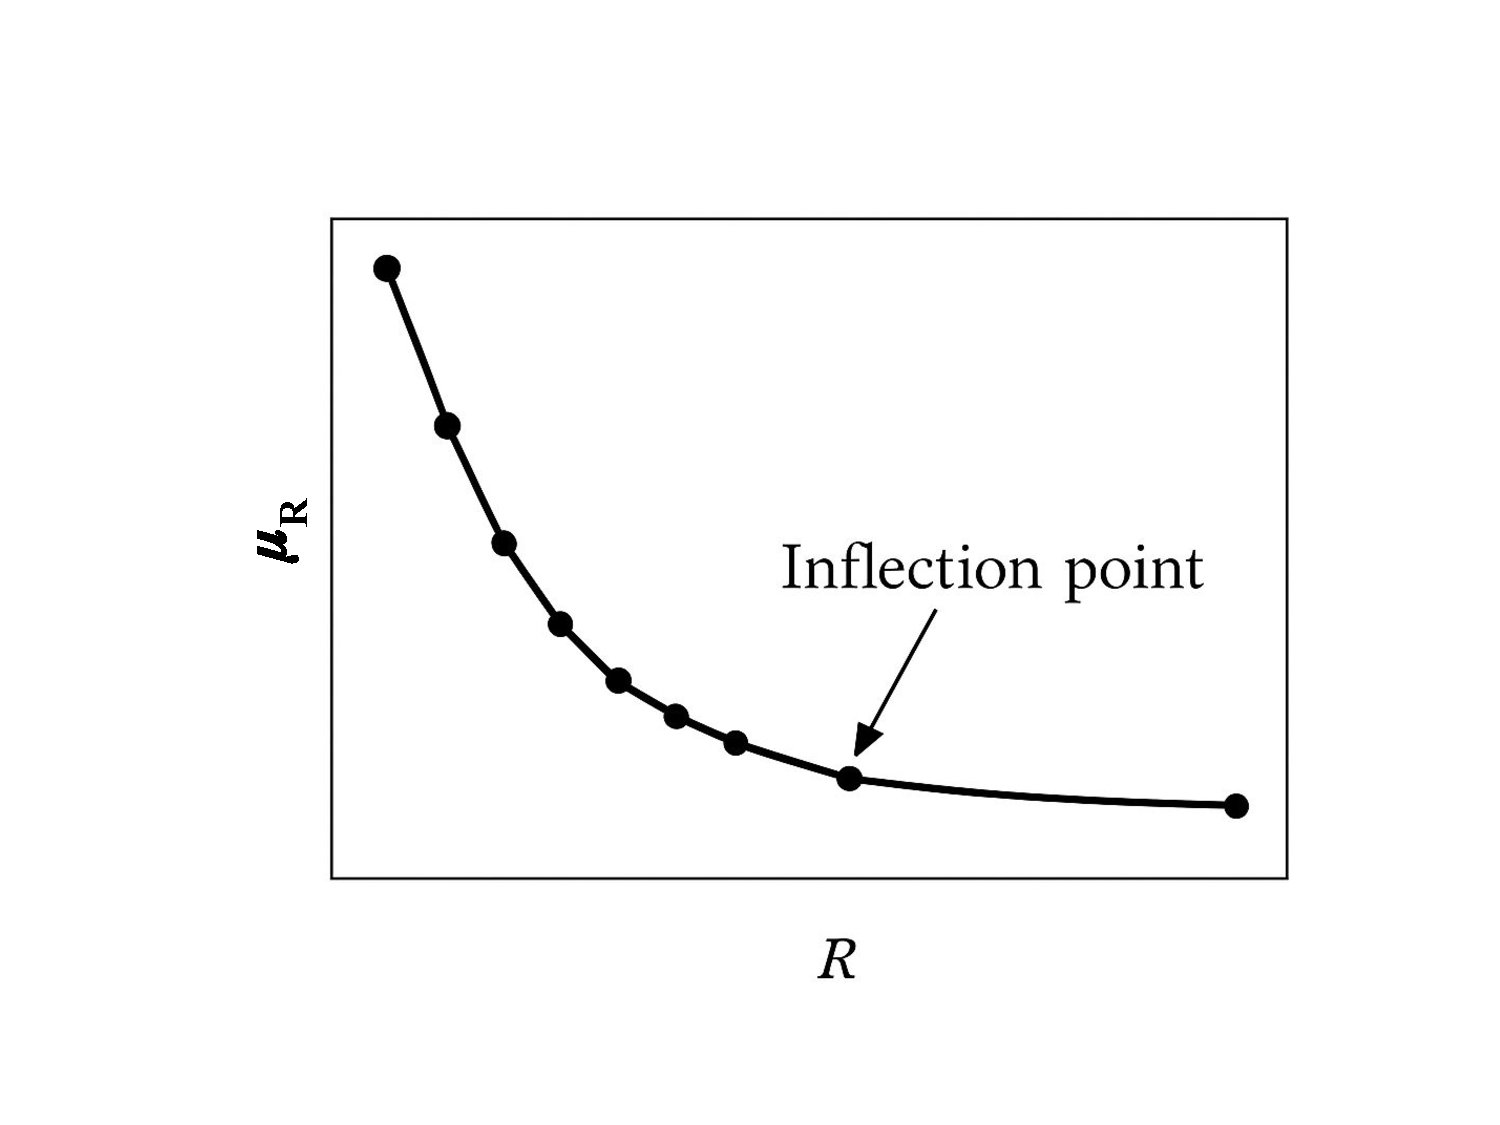
\includegraphics[clip, trim=0.5cm 2.5cm 0.5cm 3.0cm, width=0.9\textwidth]{images/elbow_plot.pdf}
% \caption{
% Elbow analysis of the mean weighted proximity distance $\mu_R$ as a function of the number of random simulations $R$. 
% The inflection point marks the threshold of distributional convergence, beyond which additional simulations yield negligible improvement in baseline stability.
% }
% \label{fig:elbow_plot}
% \end{figure}
The convergence point confirms that the null distribution provides a statistically reliable baseline for assessing charger placement performance relative to random allocation. By comparing the observed proximity metric of the real network to this stabilized null model, statistical significance is evaluated to determine whether the charger network exhibits spatial alignment with \gls{bev} activity corridor zones.
The hypothesis test evaluates whether the real network aligns with ridge-path activity better than random:
\begin{eqnarray}
H_0\!:\! & \mathrm{WPD}_{\mathrm{real}} \sim \mu_R & \quad \text{(no improvement over random)}, \\[4pt]
H_A\!:\! & \mathrm{WPD}_{\mathrm{real}} < \mu_R & \quad \text{(better-than-random alignment)}.
\label{eq:hypothesis_test}
\end{eqnarray}
% Define the empirical $p$-value as
% \begin{align}
% p_{\text{perm}}
% \;=\;
% \frac{1 + \sum_{r=1}^{R} \mathbf{1}\!\left\{\mathrm{WPD}(\mathcal{V}^{Ch}_{\mathrm{random,r}}) \le \mathrm{WPD}_{\mathrm{real}}\right\}}
%      {R + 1},
% \label{eq:p_perm}
% \end{align}
% which is valid without distributional assumptions. Reject $H_0$ at level $\alpha$ if $p_{\text{perm}} \le \alpha$. The parameter $\alpha$ denotes the predefined significance level of the hypothesis test, representing the probability of rejecting the null hypothesis $H_0$ when it is in fact true:
% \begin{align}
% \alpha \;=\; \Pr(\text{reject } H_0 \mid H_0 \text{ is true}).
% \end{align}
% In practical terms, $\alpha$ specifies the maximum tolerated false-positive rate when inferring non-random spatial alignment.  
% A smaller $\alpha$ imposes stricter evidence requirements, reducing the likelihood of false discovery but increasing the risk of overlooking genuine alignment.  
% In this analysis, $\alpha = 0.05$ was adopted to strike a balance between statistical rigor and sensitivity, consistent with conventional standards in spatial and transportation research.
% Let
% \begin{align}
% \mu_R \;=\; \frac{1}{R}\sum_{r=1}^R \mathrm{WPD}(\mathcal{C}_r),
% \qquad
% \sigma_R^2 \;=\; \frac{1}{R-1}\sum_{r=1}^R\bigl(\mathrm{WPD}(\mathcal{C}_r)-\mu_R\bigr)^2.
% \end{align}
% A standardization for interpretability is
% \begin{align}
% z \;=\; \frac{\mathrm{WPD}_{\mathrm{obs}} - \mu_R}{\sigma_R},
% \end{align}
% with (approximate) one-sided $p$-value $p_z = \Phi(z)$ when $\mathcal{N}$ is near-normal.\footnote{Use \eqref{eq:p_perm} for inference; $z$ is for effect interpretation.}
% \paragraph{Effect size (probability of superiority).}
% Let $\mathrm{rank}(\mathrm{WPD}_{\mathrm{obs}})$ be the rank among $\{\mathrm{WPD}_{\mathrm{obs}}, \mathrm{WPD}(\mathcal{C}_1),\dots,\mathrm{WPD}(\mathcal{C}_R)\}$ (1 = best).
% The common-language effect size is
% \begin{align}
% \pi \;=\; \mathbb{P}\!\left(\mathrm{WPD}_{\mathrm{obs}} < \mathrm{WPD}(\mathcal{C}_r)\right)
% \;\approx\;
% \frac{R + 2 - \mathrm{rank}(\mathrm{WPD}_{\mathrm{obs}})}{R+1},
% \end{align}
% interpretable as the fraction of random draws outperformed by the real network.
% \paragraph{Decision rule.}
% Conclude \emph{statistically significant spatial alignment} (non-random placement aligned to ridge-path demand) if $p_{\text{perm}} \le \alpha$ (e.g., $\alpha=0.05$). Report $(p_{\text{perm}}, z, \pi)$ for completeness.
% This evaluation is grounded in the ridge-path \gls{bev} activity representation introduced in Section~\ref{sec:Ridge paths}, which captures \gls{bev} count intensity along arterial corridor zones. 
Integrating mobility-based activity structure with the null distribution framework enables a rigorous statistical test of charger network intentionality, reflecting the extent to which the spatial configuration of chargers exhibits purposeful alignment with \gls{bev} activity corridor zones rather than patterns arising from random placement, forming the empirical foundation for subsequent analyses of efficiency, equity, and spatial optimization.

% Optional linking sentence to next section
% This analysis establishes the statistical foundation for the empirical results presented in Section~\ref{subsec:evaluation_results}.


% The proposed WPD offers practical benefits in a single, interpretable construct: (i) \emph{joint supply--demand weighting}, where distances are modulated by EV demand intensity and charger capacity to highlight consequential gaps; (ii) \emph{network realism}, since hop-based paths respect the arterial topology and avoid misleading Euclidean shortcuts; (iii) a \emph{benchmarkable scalar} that enables direct comparison of deployment scenarios across space and time; and (iv) \emph{diagnostic by-products}, as nearest-charger assignments and path lengths per ridge support spatial audits and equity analyses.

% \subsection{Meso-Level Planning Toolkit}
% The integration of corridor-aligned zoning, ridge-path extraction, and graph-based
% proximity metrics produces a meso-level planning toolkit. This framework bridges
% macro-level adoption forecasting and micro-level site optimization. It enables planners
% to detect misalignments between demand corridors and existing charging networks,
% prioritize corridors for infrastructure rollout, and generate inputs for equity and
% allocation studies at finer scales.


 

% ======================
% Case Study
% ======================
\section{Case study}
\label{sec:case_study}
\subsection{Study area and datasets}
\label{subsec:study_area}
This study focuses on the City of Toronto, Canada, employing arterial corridor zones derived in Section~\ref{sec:derived_AZ}. 
The empirical analysis draws upon three primary datasets: 
(i) The \gls{tcl}, obtained from the City of Toronto Open Data Portal, which provides comprehensive road geometry and functional classifications summarized in Table~\ref{tab:road_classes}; 
(ii) \glspl{fsa}, acquired from Statistics Canada’s Spatial Data Repository, which delineate the urban study boundary and represent the most disaggregated spatial level at which \gls{bev} registration data are available; and 
(iii) FLO \gls{dcfc} stations, sourced from \gls{afdc} database. 
Because the \gls{afdc} dataset does not specify per-port power ratings, a uniform nominal charging power of $100\,\mathrm{kW}$ per port was assumed across all installations. 
% The spatial distribution of these stations was subsequently mapped in accordance with Equation~\ref{eq:charger_mapping}. 

All spatial analyses were conducted using \texttt{QGIS v3.34} and Python \texttt{v3.11}, employing the \texttt{geopandas} and \texttt{networkx} libraries. 
Computations were performed on a 64-bit Windows~10 workstation equipped with an Intel\textsuperscript{\textregistered} Core\textsuperscript{TM} i7-8700T CPU @ 2.40\,GHz, 16\,GB RAM, and integrated Intel UHD Graphics~630. 
Data were stored on a 512\,GB NVMe SSD. 
Typical preprocessing and spatial intersection operations over 234 arterial regions completed within several minutes.
\subsection{Arterial zone extraction}\label{subsec:az_extraction}
The proposed arterial zoning algorithm successfully transformed the \gls{tcl} and \gls{fsa} boundaries, as illustrated in Figure \ref{fig:TCN_FSA}, into a topologically coherent and spatially continuous set of arterial zones shown in Figure \ref{fig:arterial_zones}, suitable for meso-scale spatial analysis. All layers are projected to UTM 17N (EPSG:32617) per Definition~\ref{def:projection}.  Starting from over 40{,}000 individual road segments in the \gls{tcl} dataset, the filtering and connectivity refinement stages reduced the network to approximately 1{,}200 major arterial links. This selective extraction preserved the primary mobility corridors that shape \gls{bev} travel demand while excluding expressway, local and collector roads that fragment the network topology. 
\begin{figure}[htbp]
  \centering
  \captionsetup{justification=centering}
  % (a)
  \begin{subfigure}[t]{0.49\textwidth}
    \centering
    \includegraphics[width=\linewidth,
                     height=0.6\textheight,
                     keepaspectratio,
                     pagebox=cropbox]{images/Toronto_Centreline_JournalMap.pdf}
    \caption{\gls{tcl} dataset, representing the primary road infrastructure used for arterial zones delineation.}
    \label{fig:TCN}
  \end{subfigure}\hfill
  % (b)
  \begin{subfigure}[t]{0.49\textwidth}
    \centering
    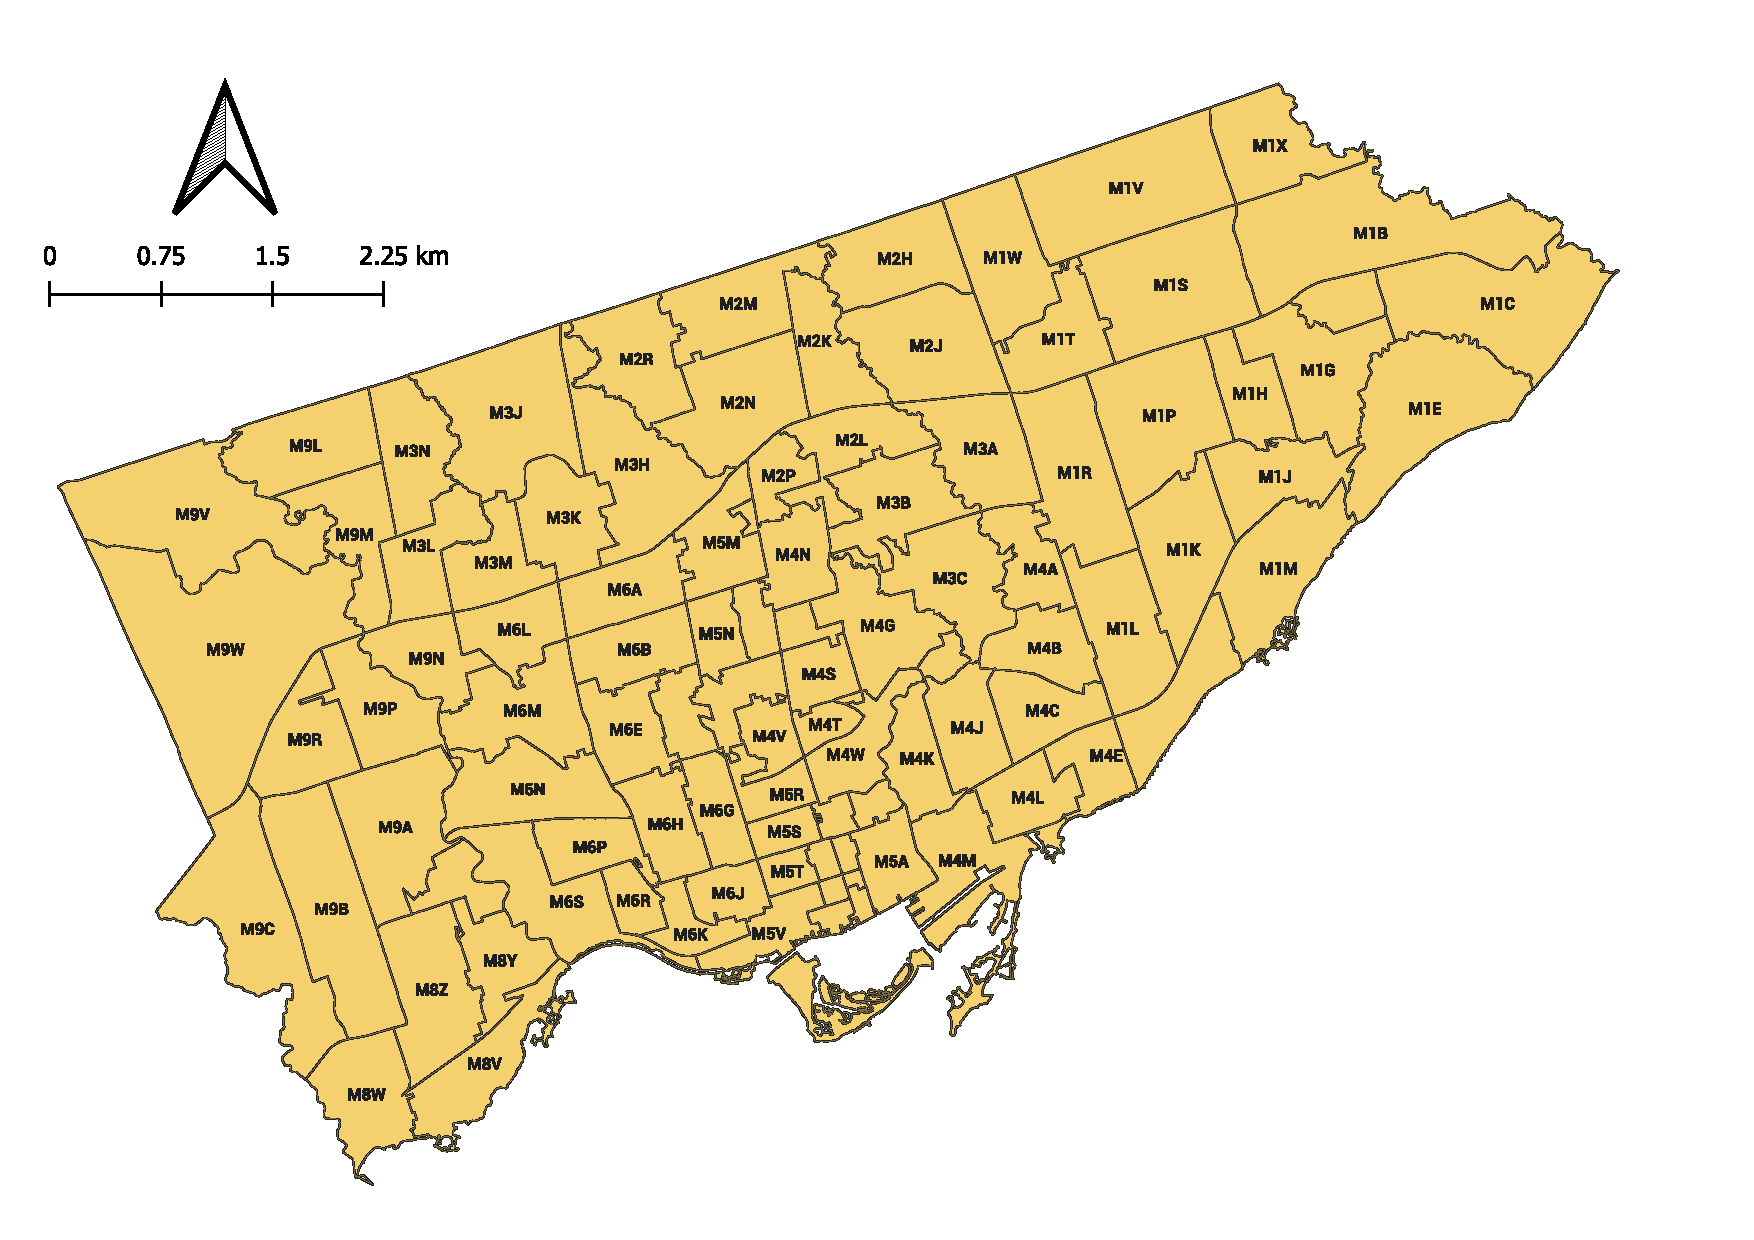
\includegraphics[width=\linewidth,
                     height=0.44\textheight,
                     keepaspectratio,
                     pagebox=cropbox]{images/Toronto_FSA_JournalMap.pdf}
    \caption{\gls{fsa} boundaries, representing the finest spatial level at which \gls{bev} registration data are available in the study area.}
    \label{fig:FSA}
  \end{subfigure}

  \caption{Input geospatial datasets for the arterial zoning algorithm: (a) \gls{tcl} dataset; (b) \gls{fsa} boundaries.}
  \label{fig:TCN_FSA}
\end{figure}

The polygonization process, limited by the dissolved \glspl{fsa} boundaries, produced 234 contiguous arterial zones throughout the urban region, as illustrated in Figure \ref{fig:arterial_zones}.
% Each zone is topologically closed, free of overlaps or sliver geometries, and uniquely labeled according to Equation~\eqref{eq:AZ_final}. 
The resulting zones exhibit a strong spatial alignment with the major arterial roads structure of Toronto, capturing the city’s major east-west and north-south travel corridors such as Bloor, Danforth, Eglinton, Finch, and Lawrence avenues.
% The geometric refinement step removed 17 micro-polygons below the area threshold (0.02~km$^2$), ensuring that all final zones represent meaningful planning units. The average arterial zone area is 2.8~km$^2$, with a standard deviation of 1.6~km$^2$. Larger zones are concentrated in the suburban periphery where arterial spacing increases, while smaller, denser zones emerge in the downtown core where road intersections are frequent and block sizes are smaller.
The final arterial zoning layer  provides a robust spatial framework for subsequent \gls{bev} charging activity modeling and accessibility analysis. Each zone is readily intersectable with demographic, traffic, or infrastructure datasets, enabling consistent aggregation and disaggregation across urban subsystems. Compared to \gls{fsa} or census-based partitions, the arterial zones offer improved geometric regularity and direct correspondence to transportation corridors, which are essential for modeling vehicle-based mobility and charger utilization.
\begin{figure}[htbp]
  \centering
  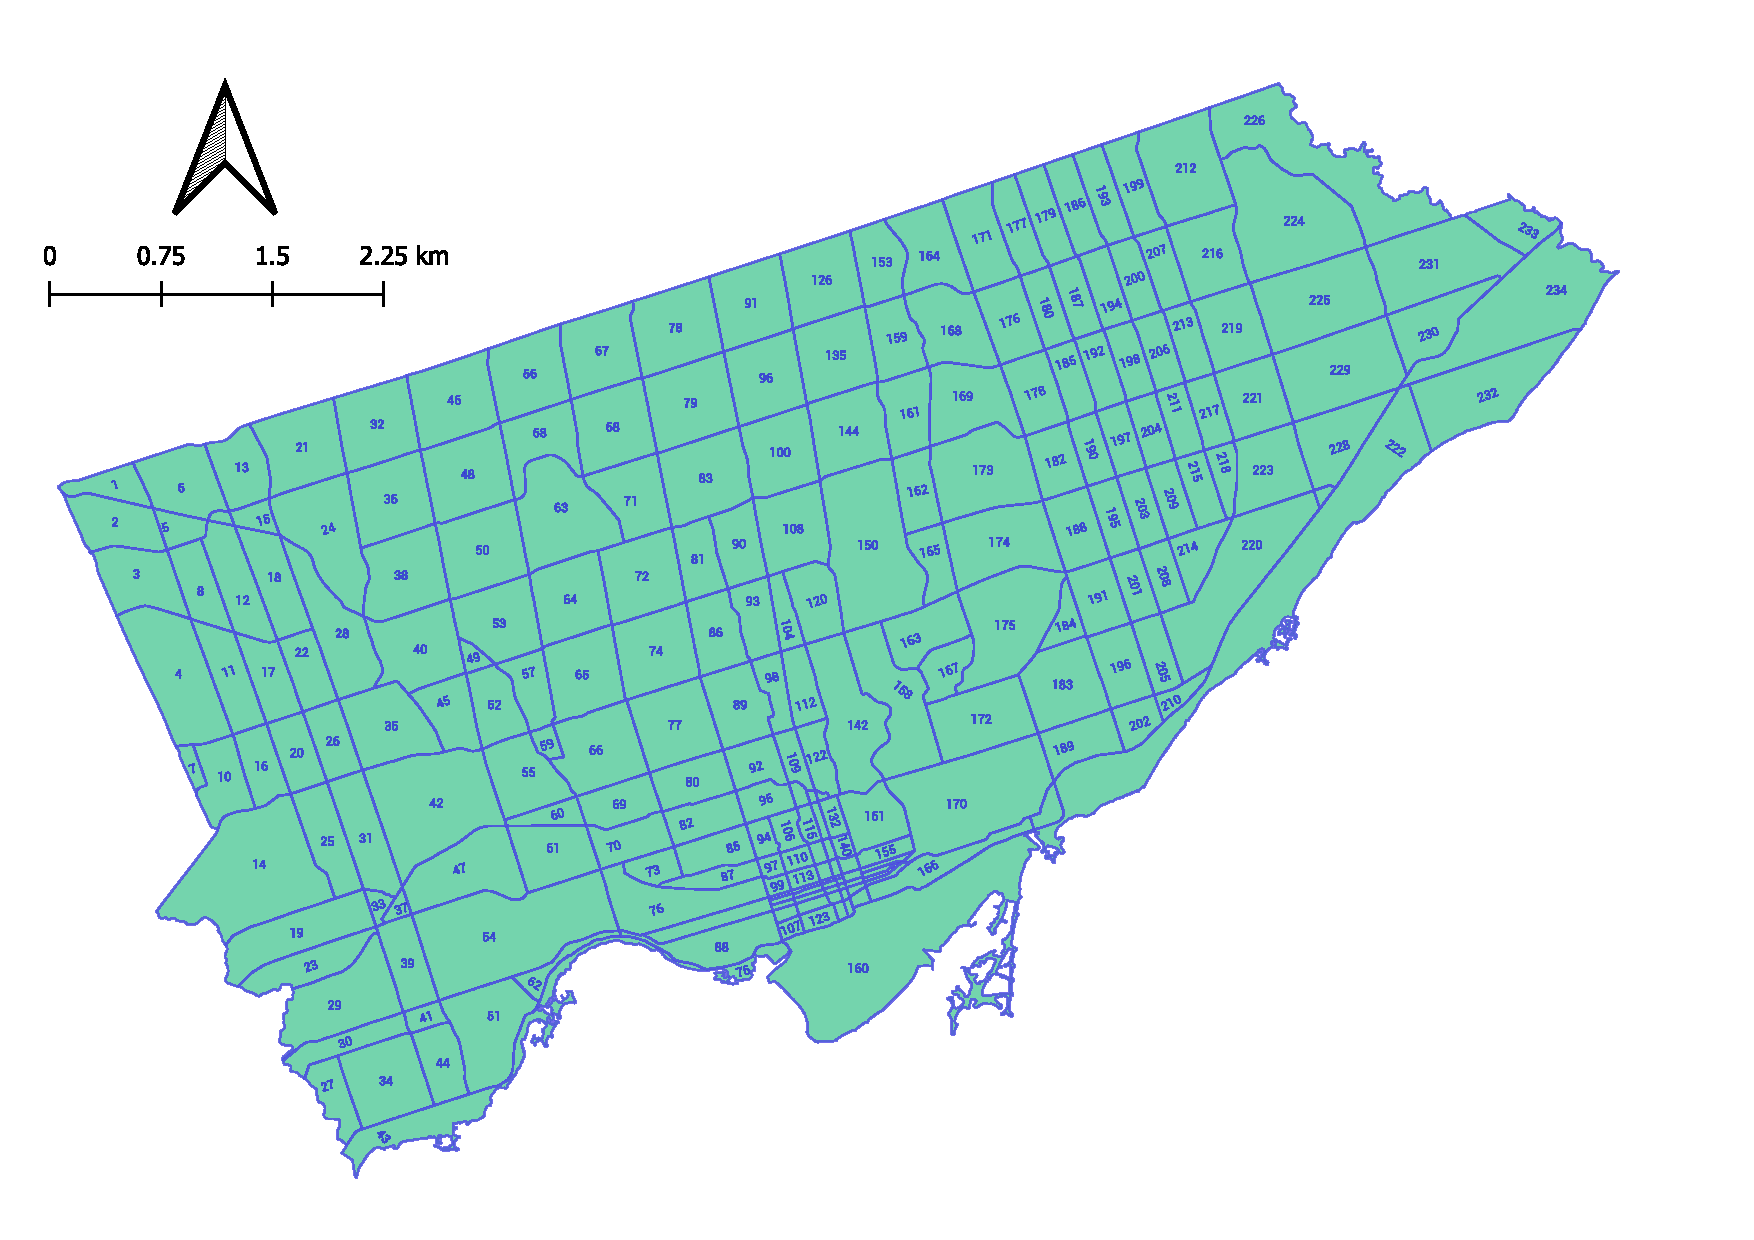
\includegraphics[width=0.75\linewidth]{images/Toronto_arterial_zones_JournalMap.pdf}
  \caption{Derived arterial zones for the City of Toronto.}
  \label{fig:arterial_zones}
\end{figure}
\subsection{Arterial zones' \gls{bev} densities}
\label{subsec:EV_density_results}
The redistribution procedure described in Section~\ref{sec:Ev_density_for AZ} produces spatial field of  \gls{bev} densities aligned with the arterial corridor zones. 
% Figure~\ref{fig:arterial_ev_density} illustrates the resulting distribution of smoothed BEV densities $\tilde{\rho}^{\mathrm{Ar}}_{j}$ across the arterial zones of Toronto, as computed from~\eqref{eq:EV_density_nhop_weighted}. 
By intersecting the \gls{fsa} polygons with the derived arterial zones, as shown in Figure~\ref{fig:fsa_arterial_intersection}, \gls{bev} ownership counts are proportionally divided based on the resulting intersection areas.
% This operation follows the allocation rule in Equation~\eqref{eq:EV_allocation_intersection} and formally described in~\eqref{eq:ev_counts_for_intersection}, ensuring that the resulting densities capture corridor-level spatial variation rather than administrative artifacts.
% The area-weighted allocation yields a substantial refinement of spatial detail. 
\begin{figure}[!ht]
  \centering
  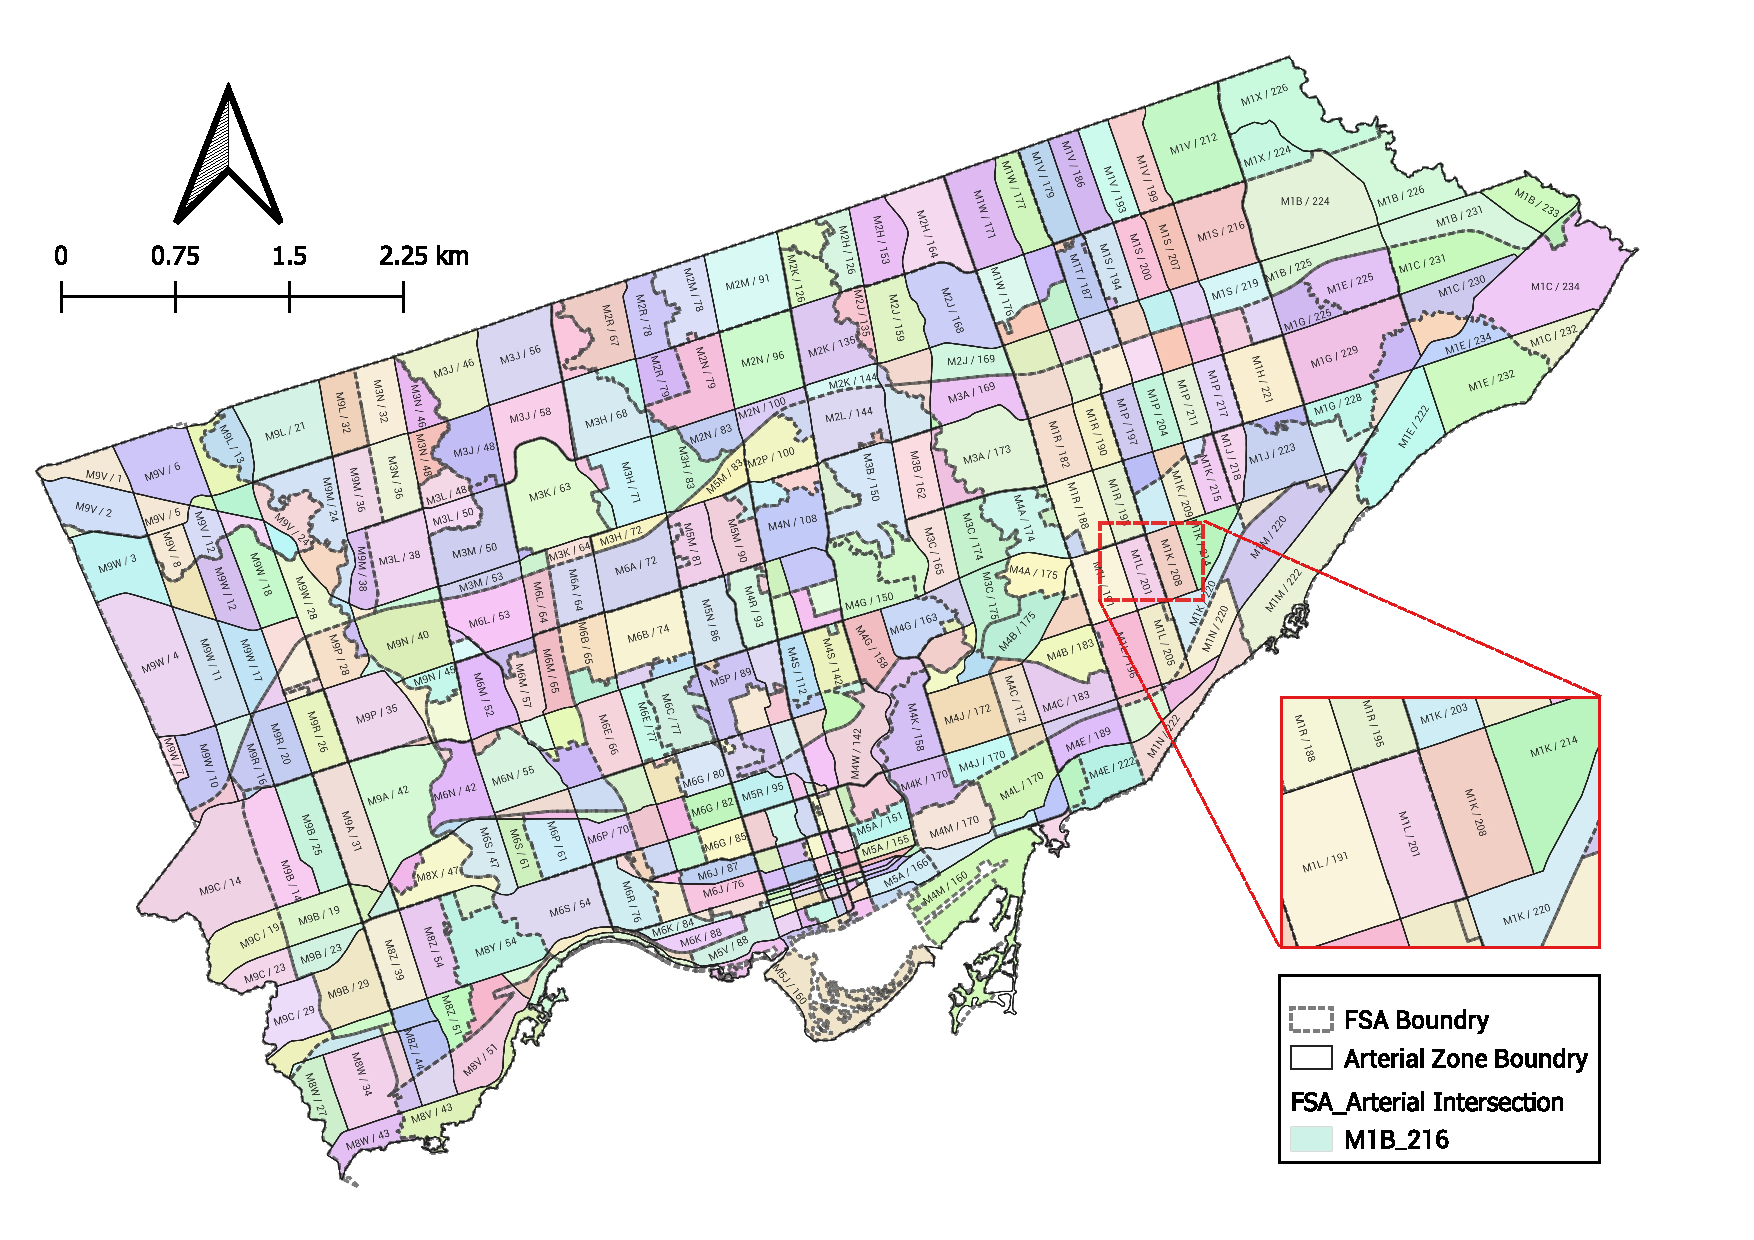
\includegraphics[width=0.7\textwidth]{images/Toronto_FSA_Arterial_intersections_JournalMap.pdf}
  \caption{Intersection between \glspl{fsa} and arterial zones for redistributing \gls{bev} ownership counts.}
  \label{fig:fsa_arterial_intersection}
\end{figure}
To recover ownership counts of \gls{bev} at the arterial scale, the allocations at each intersection are aggregated across all \glspl{fsa} that intersect each arterial zone \gls{ZArj}, as defined in Equation~\eqref{eq:EV_aggregate_arterial}.
% This aggregation step bridges the statistical domain of administrative reporting and the topological domain of arterial mobility corridors. 
It converts ownership data from the \gls{fsa} zoning schema into a spatial representation of BEV concentration defined over the arterial zoning schema, ensuring consistency with the network structure utilized in charger siting and accessibility analyses.
% While raw FSA-level data display large, discrete blocks of BEV ownership, the arterial-level representation reveals a more nuanced pattern. 
% High-density segments tend to cluster around central and midtown corridors, including Yonge Street, Bloor–Danforth, and Eglinton Avenue, corresponding to regions with greater residential and mixed-use intensity. 
% Peripheral arterial regions exhibit lower normalized densities, particularly toward Scarborough and the northwest industrial corridors, reflecting both lower residential BEV ownership and limited charging demand potential.  
% From~\eqref{eq:EV_aggregate_arterial}, and with  \gls{AAr} defined in~\eqref{eq:artertal_zones_area}, the absolute ownership counts are converted into intensity measures according to Equation~\eqref{eq:EV_density_arterial}. The resulting \gls{bev} density \gls{rhoAr} enables direct comparison of concentration levels across arterial zones of unequal size. 
% The normalization procedure~\eqref{eq:EV_density_norm} scales the densities to the unit interval, facilitating direct comparison across corridors of unequal size. 
% This enables subsequent analyses, such as charger-demand alignment, spatial equity assessment, and ridge-path demand extraction, to be performed without bias from differing region areas or total \gls{bev} counts. 
% Following normalization, a spatial smoothing procedure is applied to reduce small-area noise and account for spatial spillovers across adjacent arterial zones. As described in Equation~\eqref{eq:EV_density_nhop_weighted}, each arterial-zone \gls{bev} density is replaced by a weighted local average computed over its neighbours. The smoothing employs an $n$-hop distance structure, where the densities of neighbouring zones within $n$ steps contribute according to a convex weight vector $\mathbf{w}$. In this analysis, the hyperparameters were set to $n=1$ and $w_{1}=0.5$, assigning equal influence to each zone and its immediate neighbours. 
% This one-hop smoothing preserves local variation while attenuating random fluctuations caused by boundary effects or data irregularities. The resulting smoothed-density heatmap is shown in Figure~\ref{fig:ev_density_heatmap}; the empirical distribution is summarized by the histogram in Figure~\ref{fig:ev_density_hist} and the descriptive statistics in Table~\ref{tab:ev_density_stats}.
Absolute ownership counts are first converted into arterial-zone intensity measures, then normalized to the unit interval to enable unbiased comparison across arterial zones. The normalized densities are subsequently smoothed using a one-hop, \gls{nHop} $=1 $, weighted averaging procedure with weights $w_{0}=1$ and $w_{1}=0.5$, which mitigates local noise and boundary effects while preserving spatial variation. The resulting smoothed \gls{bev} density distribution is illustrated in Figure~\ref{fig:ev_density_heatmap}, with summary statistics reported in Figure~\ref{fig:ev_density_hist} and Table~\ref{tab:ev_density_stats}.

\begin{figure}[htbp]
  \centering
  \captionsetup{justification=centering}
  % (a) Heatmap
  \begin{subfigure}[t]{0.49\textwidth}
    \centering
    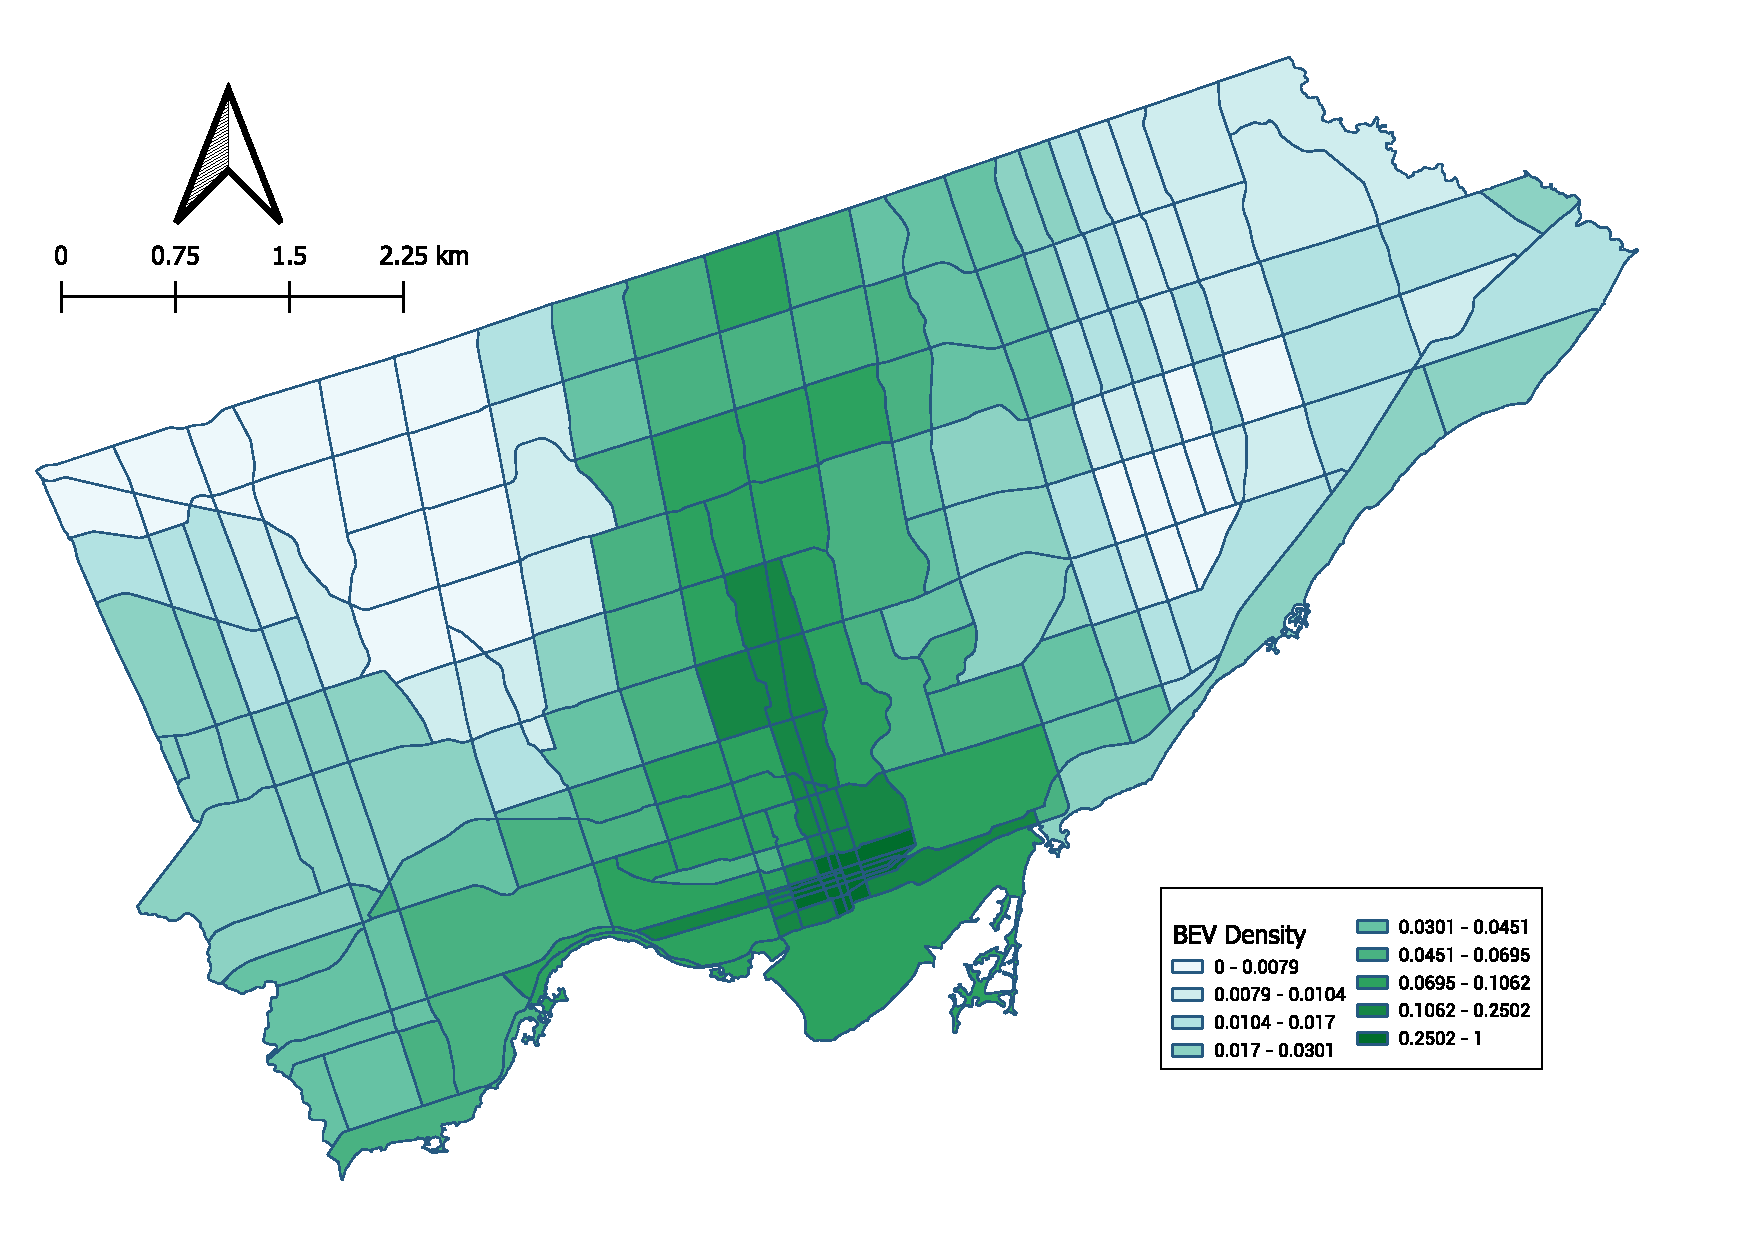
\includegraphics[width=\linewidth,
                     height=0.55\textheight,
                     keepaspectratio,
                     pagebox=cropbox]{images/Toronto_arterial_zones_BEV_densities_JournalMap.pdf}
    \caption{Smoothed \gls{bev} density heatmap across Toronto’s arterial zones. 
    Colors encode \gls{rhoArSmooth} values derived from one-hop smoothing.}
    \label{fig:ev_density_heatmap}
  \end{subfigure}\hfill
  % (b) Histogram
  \begin{subfigure}[t]{0.49\textwidth}
    \centering
    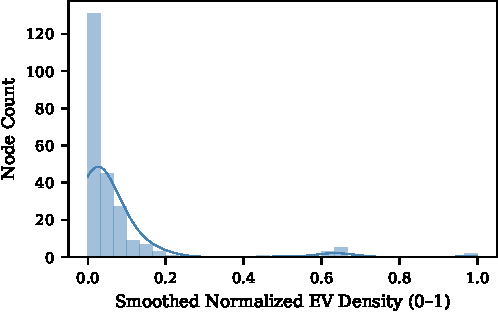
\includegraphics[width=\linewidth,
                     height=0.55\textheight,
                     keepaspectratio,
                     pagebox=cropbox]{images/ev_density_distribution.pdf}
    \caption{Histogram showing the distribution of smoothed \gls{bev} densities \gls{rhoArSmooth} across arterial zones.}
    \label{fig:ev_density_hist}
  \end{subfigure}

  \caption{Spatial and statistical representation of smoothed \gls{bev} densities across arterial zones: 
  (a) heatmap of $\tilde{\rho}^{\mathrm{Ar}}_{j}$ values; 
  (b) corresponding empirical distribution.}
  \label{fig:ev_density_visuals}
\end{figure}

% s


% The resulting distribution of $\widehat{\rho}^{\mathrm{Ar}}_{j}$ exhibits strong spatial autocorrelation (high–high clustering), consistent with corridor-continuous demand patterns rather than random dispersion.

% Overall, the derived arterial EV density layer forms a meso-level representation of ownership-driven demand potential. 
% It bridges the gap between coarse administrative data and the fine-grained spatial logic of urban mobility corridors, providing a consistent quantitative foundation for charger placement, network optimization, and equity-driven infrastructure planning.

% \begin{figure}[htbp]
%   \centering
%   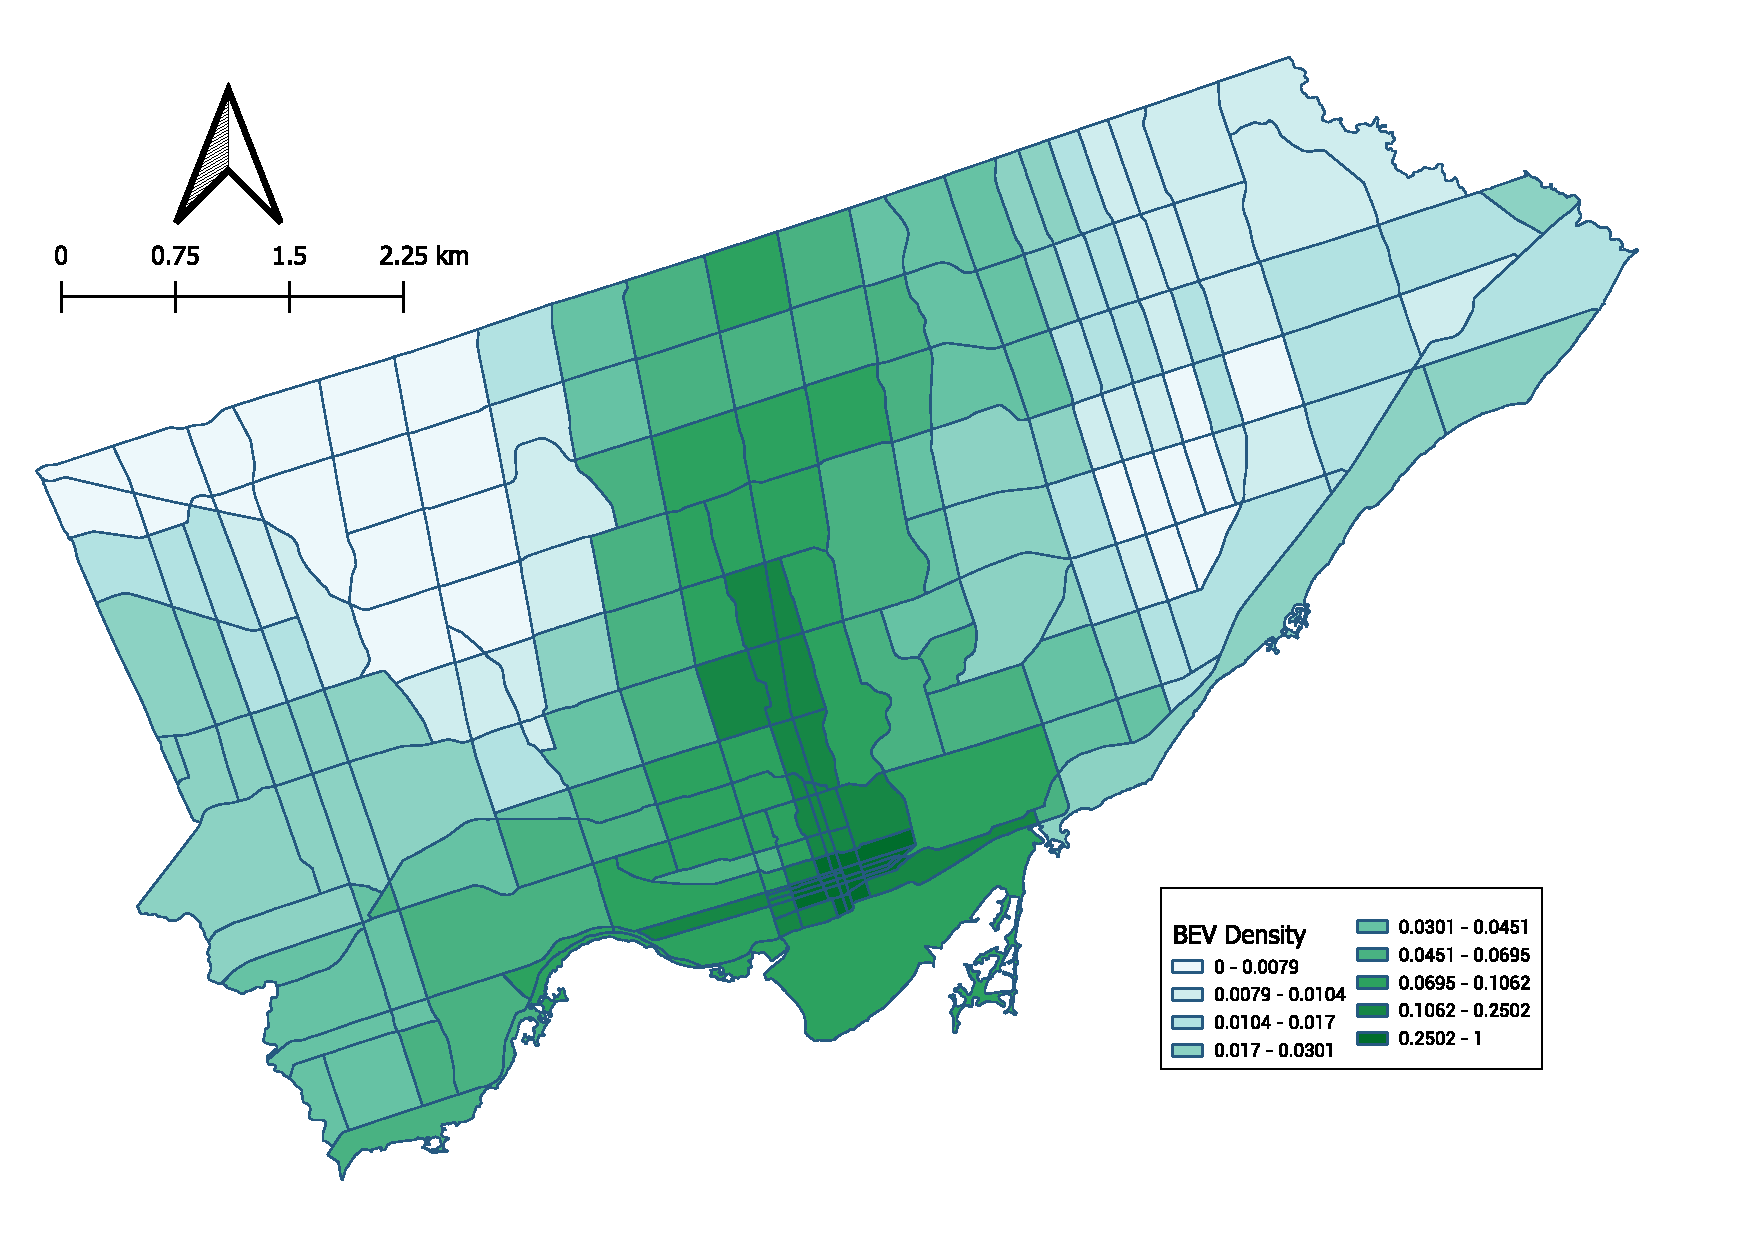
\includegraphics[width=0.9\textwidth]{images/Toronto_arterial_zones_BEV_densities_JournalMap.pdf}
%   \caption{Smoothed BEV density ($\tilde{\rho}^{\mathrm{Ar}}_{j}$) across arterial zones in the City of Toronto.}
%   \label{fig:arterial_ev_density}
% \end{figure}

% \subsection{Preprocessing and Spatial Setup}
% \label{subsec:preprocessing}
% EV counts are dasymetrically disaggregated from FSAs to intersection regions (Eq.~\eqref{eq:EV_allocation_intersection}) and aggregated to arterial zones (Eq.~\eqref{eq:EV_aggregate_arterial}), then normalized (Eq.~\eqref{eq:EV_density_norm}).
\subsection{Graph constraction}
\label{subsec:hop_distance_results}

The planar adjacency graph defined in Equation~\eqref{eq:urban_graph} yields a connected and topologically coherent representation of Toronto's arterial zones, as illustrated in Figure~\ref{fig:local_maxima_map}. 
Each vertex corresponds to the centroid of an arterial polygon, and edges connect zones that share a nonzero boundary segment. 
The resulting graph contains $|$\gls{VertexSet}$| = 234$ vertices and $|$\gls{EdgeSet}$| = 479$ undirected edges, as shown in Table~\ref{tab:graph_overview}.
% \begin{figure}[!ht]
%   \centering
%   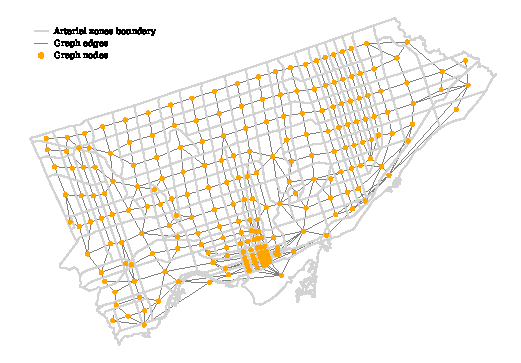
\includegraphics[width=0.85\textwidth]{images/toronto_arterial_graph.pdf}
%   \caption{Adjacency graph of Toronto's arterial zones. 
%   Nodes correspond to zone centroids and edges connect zones sharing common boundaries.}
%   \label{fig:arterial_graph}
% \end{figure}

%========================
% Graph-Theoretic Analysis
%========================
\subsubsection{Graph-theoretic analysis of the arterial adjacency network}
\label{subsec:graph_analysis}
The edge density is low $0.0176$, indicating a sparse mesh, expected for an adjacency graph rather than a road-traffic graph. Despite sparsity, the graph is fully connected, one component, ensuring network-wide reachability.
Node degrees range from $2$ to $9$, with a median of $4$ and a mean of $4.094$. No leaves are present, leaf fraction $=0$, indicating that every zone maintains at least two distinct neighbors and thus exhibits non-fragile local connectivity. The hub set is modest, with a maximum degree of $9$, ensuring that no extreme star-like structures emerge, as shown in Table~\ref{tab:top_degree}.
Global transitivity is $0.1418$ and the average local clustering is $0.1406$, with a total of $75$ triangles. This indicates a moderate level of triadic closure, meaning that some groups of three adjacent zones form closed loops. Such local triangular connections provide short alternative paths and enhance spatial redundancy, while maintaining the network’s sparse corridor structure rather than forming overly dense clusters.
% \paragraph{Connectivity and Resilience.}
The graph has no bridges and no articulation points. Hence, removing any single edge or single node does not disconnect the network. In topological terms, the network is robust to single-point failures.
% \paragraph{Core Decomposition.}
The maximum $k$-core is $k_{\max}=3$, containing $224$ nodes ($\approx 95.7\%$ of $V$). Nearly the entire network participates in a 3-core, which signals pervasive redundancy: most zones are embedded within triads and maintain degree $\ge 3$ inside the core.
% \paragraph{Path Structure.}
On the only connected component, the average shortest path length is $7.8523$, with diameter $20$ and radius $12$. The large diameter/radius indicates an elongated, corridor-like structure at the city scale: a single site cannot provide short-hop access city-wide; multi-seed strategies are mandatory.

% \paragraph{Assortativity.}
The degree assortativity coefficient is $r = 0.0789$, indicating a weakly positive correlation between the degrees of adjacent zones. This result implies that well-connected arterial zones tend to be linked slightly more frequently with other well-connected zones, whereas sparsely connected zones are more likely to border similarly sparse ones. The absence of a pronounced hub-leaf structure indicates a balanced and non-hierarchical pattern of connectivity across the arterial zones network. Greedy modularity analysis identifies $7$ distinct communities with sizes of $[52 ,45 ,42 ,41 ,30 ,17 ,7]$, as summarized in Table~\ref{tab:communities}. These communities represent coherent meso-scale clusters of arterial connectivity and provide a natural basis for decentralized planning and staged infrastructure deployment, such as assigning at least one \gls{fc} hub to each community followed by intra-community optimization.

Node \texttt{170} ranks highest across multiple centrality measures, including degree, betweenness, closeness, and eigenvector centrality, indicating its pivotal structural role within the network. Node \texttt{222} also exhibits consistently high centrality, underscoring its importance as a secondary hub. The primary betweenness hotspots, nodes \texttt{170}, \texttt{222}, \texttt{160}, \texttt{166}, \texttt{54}, \texttt{181}, \texttt{75}, \texttt{150}, \texttt{158}, and \texttt{62}, function as inter-community gateways in the modular structure of the network, as reported in Table~\ref{tab:top_betweenness}. These nodes are strategic candidates for the placement of high-capacity facilities, as they mediate flows between communities and alleviate cross-community bottlenecks. Degree alone is insufficient to characterize such nodes, since the maximum degree remains moderate; a composite interpretation integrating betweenness, closeness, and eigenvector centralities provides a more accurate delineation of the network’s functional backbone, as summarized in Tables~\ref{tab:top_closeness}--\ref{tab:top_degree_centrality}.
Collectively, the adjacency graph serves as the backbone for subsequent ridge-path analyses, enabling the integration of topological proximity into \gls{bev} activity modeling.
\subsubsection{Ridge path extraction}
\label{subsubsec:ridge_path_results}
Ridge path extraction identifies the high-density corridor zones within the arterial adjacency graph by tracing sequences of zones that consistently maintain elevated \gls{bev} densities. 
% The procedure begins by detecting the set of local maxima defined in Equation~\eqref{eq:local_maxima_set}, representing arterial zones whose smoothed densities are greater than or equal to those of all immediate neighbours. These local maxima, shown in Figure~\ref{fig:local_maxima_map}, correspond to the peaks of the smoothed \gls{bev} density surface and delineate the starting points of potential high-demand corridors. The set of local maxima zones is 
The procedure begins by identifying local maxima, corresponding to arterial zones whose smoothed densities are greater than or equal to those of all adjacent neighbours. Identified local maxima, illustrated in Figure~\ref{fig:local_maxima_map} and summarized in Table~\ref{tab:local_maxima_set_list}, represent the peaks of the smoothed \gls{bev} density surface and serve as seed nodes for initiating ridge paths.
% \begin{align}
% \label{eq:local_maxima_set_list}
% \mathcal{M} 
%   &= 
%   \{\,3,\,11,\,18,\,47,\,51,\,104,\,109,\,132,\,95,\,207,\,221,\,180,\notag\\
%   &\quad 96,\,173,\,189,\,147,\,107,\,210,\,181,\,7,\,131\,\}.
% \end{align}
% Each local maximum serves as a seed node from which a ridge path is initiated and extended according to the density-drop condition specified in Equation~\eqref{eq:ridge_path_set}.
\begin{figure}[!ht]
  \centering
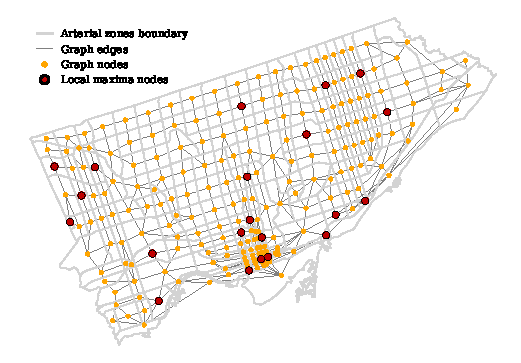
\includegraphics[width=0.7\textwidth]{images/toronto_local_maxima.pdf}
  \caption{Adjacency graph of Toronto's arterial zones, local maxima of smoothed \gls{bev} density across Toronto’s arterial zones.}
  \label{fig:local_maxima_map}
\end{figure}


Starting from each local maximum, the ridge walker, an iterative traversal algorithm, follows connected areas with a high density of \gls{bev} activity. It moves through neighboring regions where the density remains within a specified drop threshold, as outlined by the strategy-specific rules in Equations \eqref{eq:ridge_avg}-\eqref{eq:ridge_laplacian}. 
% This method allows for the continuous tracing of high-density zones from local peaks, effectively identifying the main zones of concentrated \gls{bev} activity throughout the urban network.
% The admissible set of neighbours is evaluated dynamically to ensure that the walk proceeds only along zones where densities decline gradually, preserving the continuity of high-activity zones.
Two hyperparameters govern the ridge-path extraction process: the maximum walk length \gls{L} and the drop-tolerance scaling factor \gls{eta}. The walk length is bounded by the graph diameter \gls{diamG}, set as \gls{L} $ = $ \gls{alpha}$ \times $\gls{diamG} with \gls{alpha}$ = 0.5$, limiting ridge extent to half the network span. The drop-tolerance parameter \gls{eta}$ = 0.3$ regulates the allowable descent along the density surface, smaller values enforce stricter adherence to high-density ridges, whereas larger values allow smoother, more flexible trajectories through neighbouring zones.





Five ridge-walking strategies are employed: \textsc{average}, \textsc{maximum}, \textsc{median}, \textsc{standard deviation}, and \textsc{laplacian}. Each strategy prescribes a unique rule for calculating the local drop allowance \gls{Deltat} based on the distribution of neighboring densities. These strategies offer different interpretations of ridge continuity. The \textsc{average} and \textsc{median} strategies promote balanced transitions, while the \textsc{maximum} strategy favors consistent movement along peak sequences. In contrast, the \textsc{standard deviation} and \textsc{laplacian} strategies focus on contrast-tolerant ridges that navigate through locally elevated density regions but restrict sharp declines, especially in areas with steep spatial gradients.
The minimum average density threshold \gls{rhoMin}, set at $0.0661$, corresponds to the 75th percentile of the arterial-zone density distribution, as shown in Table~\ref{tab:ev_density_stats}. This criterion ensures that only statistically significant high-density corridor zones are included.
The ridge paths extracted are visualized in Figure~\ref{fig:strategy-ridges-grid}, with each line depicting a continuous chain of arterial zones that form a corridor of high \gls{bev} activity zones.
\begin{figure*}[t]
  \centering
  % -------- Row 1: 3 panels --------
  \begin{subfigure}[t]{0.32\textwidth}
    \centering
    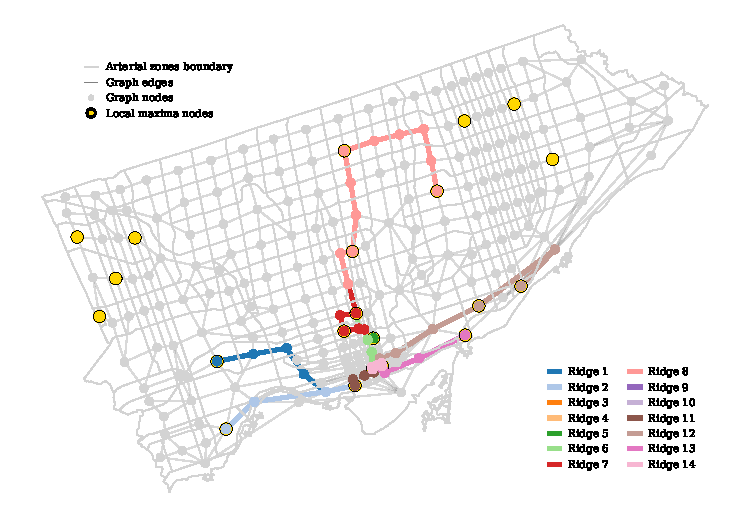
\includegraphics[width=\linewidth]{images/strategy_ridges_avg_all.pdf}
    \subcaption{Average-based ridge extraction.}
    \label{fig:ridges-avg}
  \end{subfigure}\hfill
  \begin{subfigure}[t]{0.32\textwidth}
    \centering
    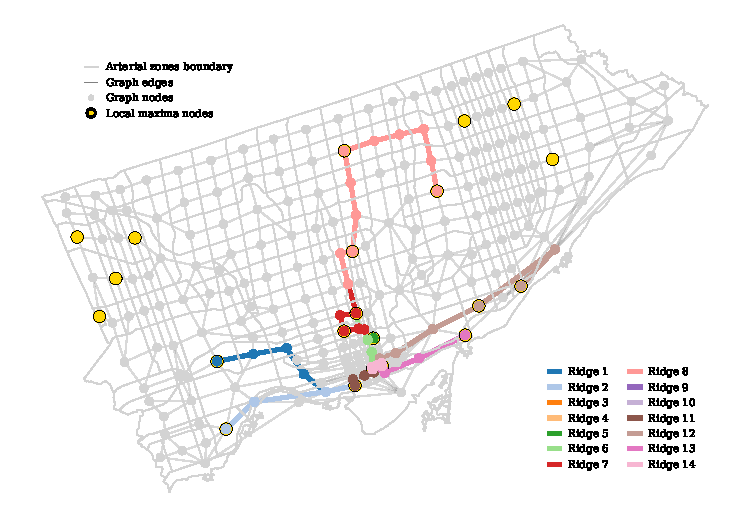
\includegraphics[width=\linewidth]{images/strategy_ridges_max_all.pdf}
    \subcaption{Maximum-based ridge extraction.}
    \label{fig:ridges-max}
  \end{subfigure}\hfill
  \begin{subfigure}[t]{0.32\textwidth}
    \centering
    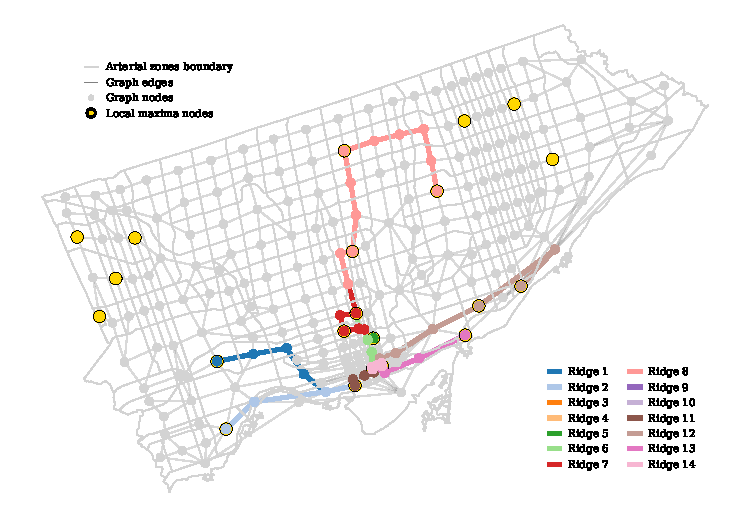
\includegraphics[width=\linewidth]{images/strategy_ridges_median_all.pdf}
    \subcaption{Median-based ridge extraction.}
    \label{fig:ridges-median}
  \end{subfigure}

  \vspace{0.6em}

  % -------- Row 2: 3 panels --------
  \begin{subfigure}[t]{0.32\textwidth}
    \centering
    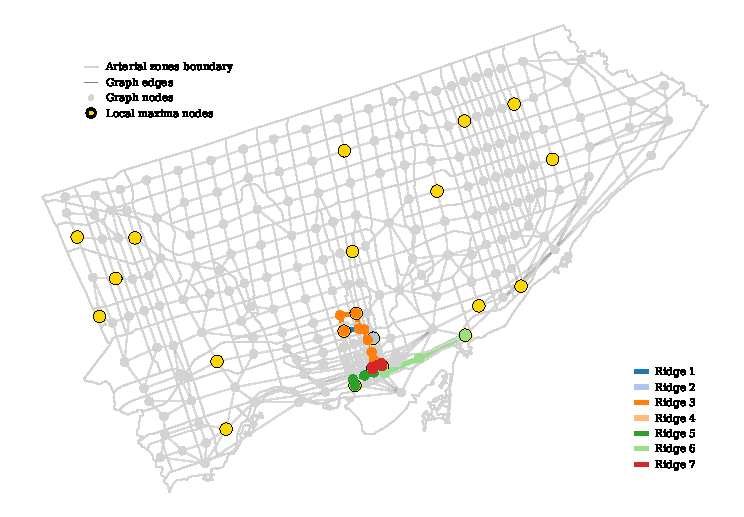
\includegraphics[width=\linewidth]{images/strategy_ridges_std_all.pdf}
    \subcaption{Standard-deviation–based ridge extraction.}
    \label{fig:ridges-std}
  \end{subfigure}\hfill
  \begin{subfigure}[t]{0.32\textwidth}
    \centering
    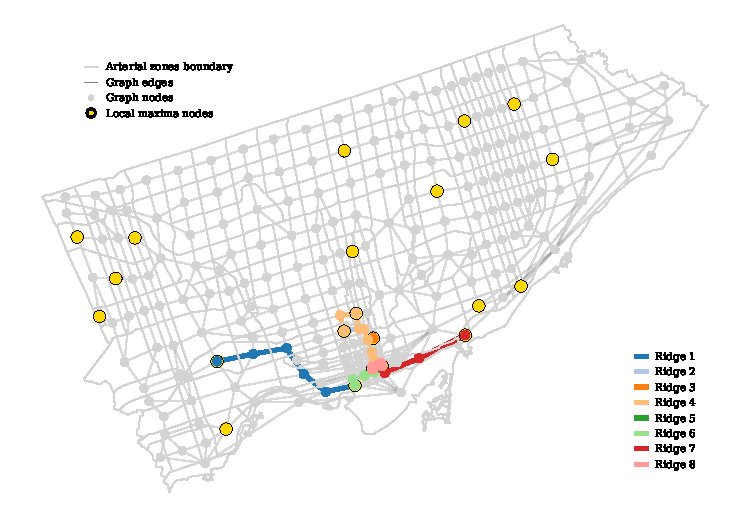
\includegraphics[width=\linewidth]{images/strategy_ridges_laplacian_all.pdf}
    \subcaption{Laplacian-based ridge extraction.}
    \label{fig:ridges-laplacian}
  \end{subfigure}\hfill
  \begin{subfigure}[t]{0.32\textwidth}
    \centering
    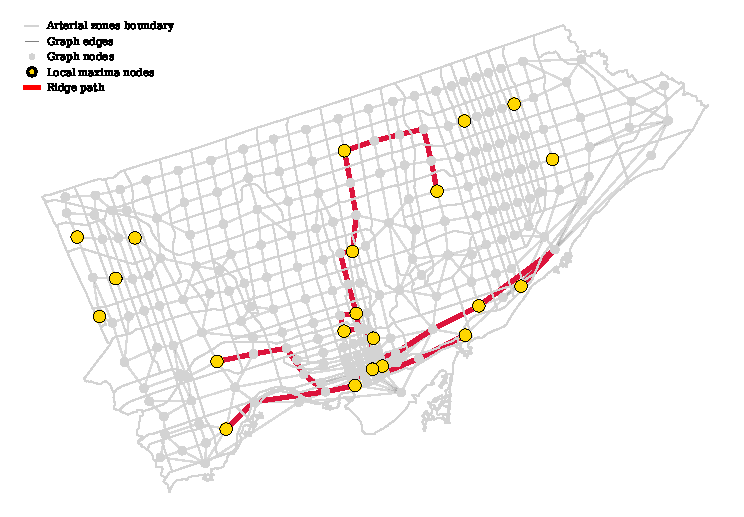
\includegraphics[width=\linewidth]{images/ridges_all_strategies_overlay_same_color.pdf}
    \subcaption{Overlay of all strategies (same ridge color).}
    \label{fig:ridges-overlay}
  \end{subfigure}

  \caption{
  Ridge-path results 
  (a) Average-based ridges; 
  (b) Maximum-based ridges; 
  (c) Median-based ridges; 
  (d) Standard-deviation–based ridges; 
  (e) Laplacian-based ridges; 
  (f) Overlay of all strategies' ridge paths drawn in a single ridge color for visual comparison.
  }
  \label{fig:strategy-ridges-grid}
\end{figure*}
\noindent
The outcomes of the ridge-path statistics for all strategies are summarized in Table~\ref{tab:ridge_summary}. The results reveal distinct behavioral patterns across the five ridge-walking strategies. The \textsc{average}, \textsc{maximum}, and \textsc{median} methods yield highly consistent ridge configurations, indicating that ridge extraction remains stable across the central-tendency formulations of the underlying \gls{bev}-density field. In contrast, the \textsc{standard deviation} and \textsc{laplacian} strategies, which are sensitive to dispersion and local contrast, produce fewer but more concentrated ridges. These methods highlight high-intensity corridors while filtering out weaker peripheral structures. Overall, central-tendency strategies favor broader coverage of regions with moderate to high density, whereas contrast-based methods delineate sharper, more dominant pathways that align with the city’s primary arterial framework.
% The results show that the average, maximum, and median strategies produce the same set of ridge paths, as illustrated in Figures~\ref{fig:ridges-avg}, \ref{fig:ridges-max}, and \ref{fig:ridges-median}, respectively. This consistency suggests that ridge extraction is reliable regardless of the central-tendency operator used for the underlying BEV-density signal. For these three strategies, each with  14  ridge paths, the mean ridge density, calculated as the average of the zone densities along each ridge path, is 0.397, while the median is 0.345. The ridge density values range from 0.078 to 1.000.
% In contrast, the \textsc{std} and \textsc{laplacian} strategies generate fewer ridge paths but with higher densities, as illustrated in Figures~\ref{fig:ridges-std} and \ref{fig:ridges-laplacian}, respectively. The \textsc{std} method produces 7 ridges with a mean of 0.559 and a median of 0.493. Meanwhile, the \textsc{laplacian} method results in 8 ridges with a mean of 0.521 and a median of 0.481, as summarized in Table~\ref{tab:ridge_summary}.
% These patterns imply that dispersion- and contrast-sensitive strategies preferentially retain persistent, high-intensity corridor zones, whereas central-tendency criteria enumerate a broader set that also includes moderate-intensity segments. 
% The \textsc{average}, \textsc{max}, and \textsc{median} methods yield the most stable ridge sets, balancing length and density preservation, whereas the \textsc{std} and \textsc{laplacian} strategies produce fewer yet higher-density, often more elongated ridges concentrated along dominant urban corridors.
% Notably, all strategies include the short, high-intensity link $147, 146$ (density $=1.000$), marking a consistent core corridor zones across strategies. 
The union of all ridge-path nodes, as defined in Equation~\eqref{eq:ridge_path_nodes}, represents the full set of arterial zones that support the mobility-based \gls{bev} activity structure, as illustrated in Figure~\ref{fig:ridges-overlay}.
% \begin{table}[htbp]
% \centering
% \caption{Extracted Ridge Nodes and Corresponding Normalized BEV Densities}
% \label{tab:ridge_ev_density}
% \setlength{\tabcolsep}{6pt}%
% \begin{minipage}[t]{0.32\linewidth}
% \vspace{0pt}%
% \centering
% \begin{tabularx}{\linewidth}{>{\centering\arraybackslash}X>{\centering\arraybackslash}X}
% \toprule
% \textbf{Node ID} & \textbf{BEV Density} \\
% \midrule
% 100 & 0.0662 \\
% 104 & 0.1067 \\
% 105 & 0.1246 \\
% 107 & 0.1263 \\
% 108 & 0.0626 \\
% 109 & 0.0996 \\
% 111 & 0.0995 \\
% 118 & 0.0960 \\
% 119 & 0.1982 \\
% 124 & 0.1405 \\
% 129 & 0.1634 \\
% 130 & 0.6356 \\
% 131 & 0.6363 \\
% 132 & 0.1470 \\
% 133 & 0.6354 \\
% 134 & 0.1658 \\
% 135 & 0.0510 \\
% 136 & 0.6311 \\
% 137 & 0.6441 \\
% 143 & 0.1280 \\
% \bottomrule
% \end{tabularx}
% \end{minipage}\hfill
% %
% \begin{minipage}[t]{0.32\linewidth}
% \vspace{0pt}%
% \centering
% \begin{tabularx}{\linewidth}{>{\centering\arraybackslash}X>{\centering\arraybackslash}X}
% \toprule
% \textbf{Node ID} & \textbf{BEV Density} \\
% \midrule
% 146 & 0.9993 \\
% 147 & 1.0000 \\
% 148 & 0.4549 \\
% 149 & 0.2031 \\
% 155 & 0.0820 \\
% 159 & 0.0432 \\
% 166 & 0.0562 \\
% 168 & 0.0433 \\
% 169 & 0.0462 \\
% 170 & 0.0447 \\
% 173 & 0.0474 \\
% 181 & 0.0597 \\
% 189 & 0.0603 \\
% 210 & 0.0205 \\
% 222 & 0.0199 \\
% 47  & 0.0567 \\
% 51  & 0.0471 \\
% 61  & 0.0513 \\
% 62  & 0.0458 \\
% 70  & 0.0482 \\
% \bottomrule
% \end{tabularx}
% \end{minipage}\hfill
% %
% \begin{minipage}[t]{0.32\linewidth}
% \vspace{0pt}%
% \centering
% \begin{tabularx}{\linewidth}{>{\centering\arraybackslash}X>{\centering\arraybackslash}X}
% \toprule
% \textbf{Node ID} & \textbf{BEV Density} \\
% \midrule
% 76  & 0.0710 \\
% 88  & 0.0968 \\
% 92  & 0.0995 \\
% 93  & 0.0995 \\
% 95  & 0.1005 \\
% 96  & 0.0873 \\
% 98  & 0.0922 \\
% \bottomrule
% \end{tabularx}
% \end{minipage}
% \end{table}



\begin{table}[!ht]
\centering
\caption{Summary of ridge-path density statistics by extraction strategy.}
\label{tab:ridge_summary}
\resizebox{\linewidth}{!}{%
\begin{tabular}{lcccccc}
\toprule
\textbf{Strategy} & \textbf{Number of Ridges} & \textbf{Mean} & \textbf{Median} & \textbf{Min} & \textbf{Max} & \textbf{Std}  \\
\midrule
\textsc{average}   & 14 & 0.397 & 0.345 & 0.078 & 1.000 & 0.249  \\
\textsc{max}       & 14 & 0.397 & 0.345 & 0.078 & 1.000 & 0.249  \\
\textsc{median}    & 14 & 0.397 & 0.345 & 0.078 & 1.000 & 0.249  \\
\textsc{std}       &  7 & 0.559 & 0.493 & 0.302 & 1.000 & 0.236  \\
\textsc{laplacian} &  8 & 0.521 & 0.481 & 0.252 & 1.000 & 0.243 \\
\bottomrule
\end{tabular}%
}
% \vspace{0.25em}

\end{table}

% \begin{table}[!ht]
% \centering
% \caption{Extracted ridge paths using the \textsc{average} strategy.}
% \label{tab:ridge_avg}
% \resizebox{\linewidth}{!}{%
% \begin{tabular}{ccc}
% \toprule
% \textbf{Ridge ID} & \textbf{Avg. Density} & \textbf{Node Sequence} \\
% \midrule
% 1 & 0.252 & 47→61→70→76→88→107→105→119→133→131→130 \\
% 2 & 0.388 & 51→62→88→107→105→119→133→131→130→137→146 \\
% 3 & 0.125 & 104→93→98→109→92→95→111→118→124→129→134 \\
% 4 & 0.302 & 109→92→95→111→118→124→129→134→136→137→146 \\
% 5 & 0.493 & 132→124→129→134→136→137→146→147 \\
% 6 & 0.302 & 95→92→109→111→118→124→129→134→136→137→146 \\
% 7 & 0.102 & 96→100→108→104→93→98→109→92→95→111→118 \\
% 8 & 0.078 & 173→169→168→159→135→96→100→108→104→93→98 \\
% 9 & 0.393 & 189→170→155→143→146→147 \\
% 10 & 1.000 & 147→146 \\
% 11 & 0.561 & 107→105→119→133→131→130→137→146→147 \\
% 12 & 0.302 & 210→222→189→170→155→143→146→147 \\
% 13 & 0.469 & 181→166→149→148→147→146 \\
% 14 & 0.786 & 131→130→137→146→147 \\
% \bottomrule
% \end{tabular}%
% }
% \end{table}

% \begin{table}[!ht]
% \centering
% \caption{Ridge paths extracted using the \textsc{max} strategy.}
% \label{tab:ridge_max}
% \resizebox{\linewidth}{!}{%
% \begin{tabular}{ccc}
% \toprule
% \textbf{Ridge ID} & \textbf{Avg. Density} & \textbf{Node Sequence} \\
% \midrule
% 1 & 0.252 & 47→61→70→76→88→107→105→119→133→131→130 \\
% 2 & 0.388 & 51→62→88→107→105→119→133→131→130→137→146 \\
% 3 & 0.125 & 104→93→98→109→92→95→111→118→124→129→134 \\
% 4 & 0.302 & 109→92→95→111→118→124→129→134→136→137→146 \\
% 5 & 0.493 & 132→124→129→134→136→137→146→147 \\
% 6 & 0.302 & 95→92→109→111→118→124→129→134→136→137→146 \\
% 7 & 0.102 & 96→100→108→104→93→98→109→92→95→111→118 \\
% 8 & 0.078 & 173→169→168→159→135→96→100→108→104→93→98 \\
% 9 & 0.393 & 189→170→155→143→146→147 \\
% 10 & 1.000 & 147→146 \\
% 11 & 0.561 & 107→105→119→133→131→130→137→146→147 \\
% 12 & 0.302 & 210→222→189→170→155→143→146→147 \\
% 13 & 0.469 & 181→166→149→148→147→146 \\
% 14 & 0.786 & 131→130→137→146→147 \\
% \bottomrule
% \end{tabular}%
% }
% \end{table}

% \begin{table}[!ht]
% \centering
% \caption{Ridge paths extracted using the \textsc{median} strategy.}
% \label{tab:ridge_median}
% \resizebox{\linewidth}{!}{%
% \begin{tabular}{ccc}
% \toprule
% \textbf{Ridge ID} & \textbf{Avg. Density} & \textbf{Node Sequence} \\
% \midrule
% 1 & 0.252 & 47→61→70→76→88→107→105→119→133→131→130 \\
% 2 & 0.388 & 51→62→88→107→105→119→133→131→130→137→146 \\
% 3 & 0.125 & 104→93→98→109→92→95→111→118→124→129→134 \\
% 4 & 0.302 & 109→92→95→111→118→124→129→134→136→137→146 \\
% 5 & 0.493 & 132→124→129→134→136→137→146→147 \\
% 6 & 0.302 & 95→92→109→111→118→124→129→134→136→137→146 \\
% 7 & 0.102 & 96→100→108→104→93→98→109→92→95→111→118 \\
% 8 & 0.078 & 173→169→168→159→135→96→100→108→104→93→98 \\
% 9 & 0.393 & 189→170→155→143→146→147 \\
% 10 & 1.000 & 147→146 \\
% 11 & 0.561 & 107→105→119→133→131→130→137→146→147 \\
% 12 & 0.302 & 210→222→189→170→155→143→146→147 \\
% 13 & 0.469 & 181→166→149→148→147→146 \\
% 14 & 0.786 & 131→130→137→146→147 \\
% \bottomrule
% \end{tabular}%
% }
% \end{table}

% \begin{table}[!ht]
% \centering
% \caption{Ridge paths extracted using the \textsc{std} strategy.}
% \label{tab:ridge_std}
% \resizebox{\linewidth}{!}{%
% \begin{tabular}{ccc}
% \toprule
% \textbf{Ridge ID} & \textbf{Avg. Density} & \textbf{Node Sequence} \\
% \midrule
% 1 & 0.302 & 109→92→95→111→118→124→129→134→136→137→146 \\
% 2 & 0.493 & 132→124→129→134→136→137→146→147 \\
% 3 & 0.302 & 95→92→109→111→118→124→129→134→136→137→146 \\
% 4 & 1.000 & 147→146 \\
% 5 & 0.561 & 107→105→119→133→131→130→137→146→147 \\
% 6 & 0.469 & 181→166→149→148→147→146 \\
% 7 & 0.786 & 131→130→137→146→147 \\
% \bottomrule
% \end{tabular}%
% }
% \end{table}

% \begin{table}[!ht]
% \centering
% \caption{Ridge paths extracted using the \textsc{laplacian} strategy.}
% \label{tab:ridge_laplacian}
% \resizebox{\linewidth}{!}{%
% \begin{tabular}{ccc}
% \toprule
% \textbf{Ridge ID} & \textbf{Avg. Density} & \textbf{Node Sequence} \\
% \midrule
% 1 & 0.252 & 47→61→70→76→88→107→105→119→133→131→130 \\
% 2 & 0.302 & 109→92→95→111→118→124→129→134→136→137→146 \\
% 3 & 0.493 & 132→124→129→134→136→137→146→147 \\
% 4 & 0.302 & 95→92→109→111→118→124→129→134→136→137→146 \\
% 5 & 1.000 & 147→146 \\
% 6 & 0.561 & 107→105→119→133→131→130→137→146→147 \\
% 7 & 0.469 & 181→166→149→148→147→146 \\
% 8 & 0.786 & 131→130→137→146→147 \\
% \bottomrule
% \end{tabular}%
% }
% \end{table}
% The ridge-path extraction framework highlights the hierarchical organization of \gls{bev} activity across arterial zones. High-activity ridges indicate the core areas of the urban \gls{bev} ecosystem, where the deployment of charging infrastructure is anticipated to have the greatest impact on vehicle utilization.
\subsection{Proximity analysis between ridge zones and the \gls{dcfc} network}
\label{subsec:results_wpd}
\noindent The graph-based proximity analysis assesses the spatial accessibility between \gls{bev} activities along arterial ridge paths and the existing FLO \gls{dcfc} network. Table~\ref{tab:flo_dcfc_full} summarizes the technical characteristics of the FLO \gls{dcfc} stations, while Figure~\ref{fig:flo_dcfc_map}  illustrates their spatial distribution throughout Toronto's arterial network. The \gls{wpd} metric is then applied to evaluate how effectively the charging supply nodes serve the ridge-path nodes within the arterial-zone graph. 
% Together, these visual and tabular summaries provide the empirical basis for subsequent proximity-based accessibility and network-alignment evaluations.
\begin{figure}[htbp]
  \centering
  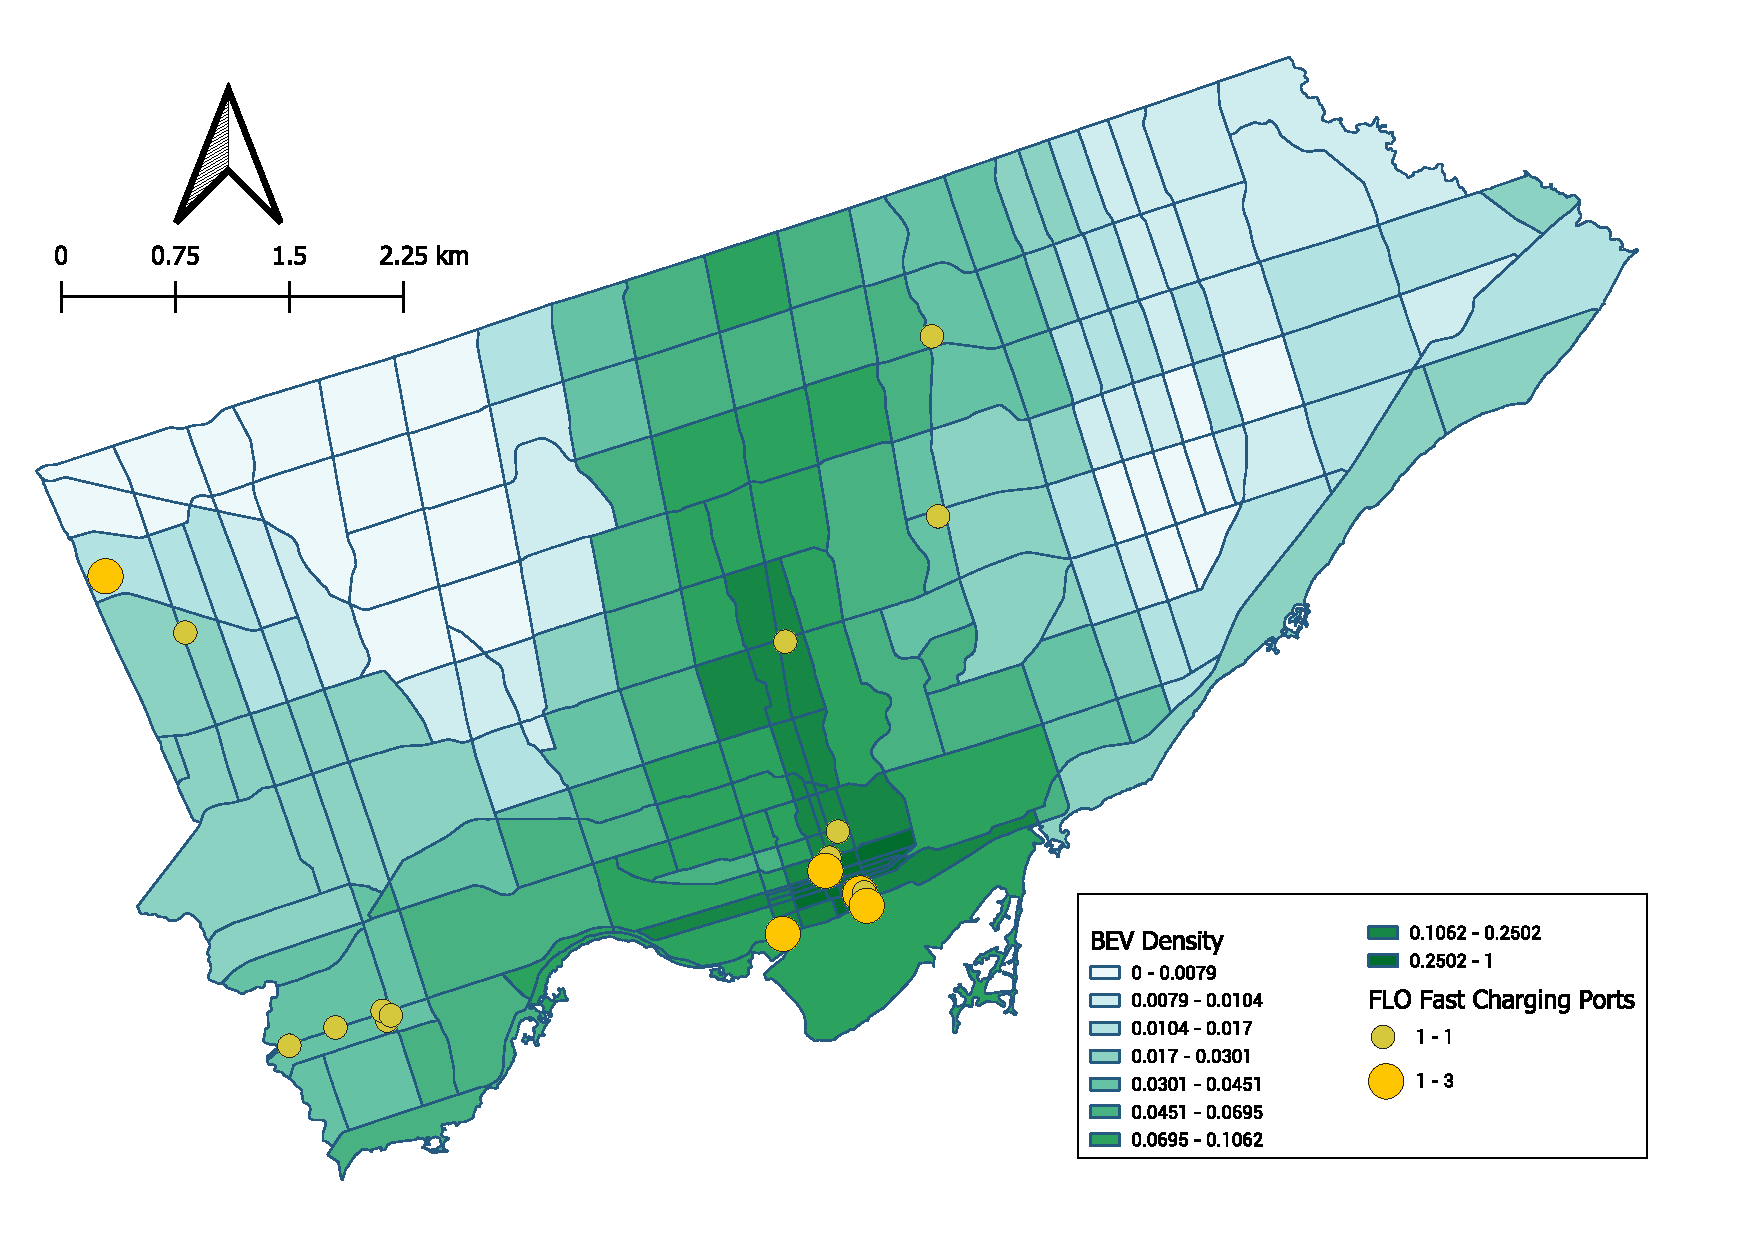
\includegraphics[width=0.7\textwidth]{images/Toronto_FLO_fastcharging_network_JournalMap.pdf}
  \caption{Spatial distribution of FLO \gls{dcfc} stations across Toronto. 
  Each point represents a station, scaled by its aggregate charging capacity (kW).}
  \label{fig:flo_dcfc_map}
\end{figure}
% \begin{table}[htbp]
% \centering
% \caption{FLO DCFC Stations in Toronto}
% \label{tab:flo_dcfc_full}
% \resizebox{\textwidth}{!}{%
% \begin{tabular}{lrrrrr}
% \toprule
% \textbf{Station Name} & \textbf{Latitude} & \textbf{Longitude} & \textbf{DC Ports} & \textbf{Per-Port (kW)} & \textbf{Station (kW)} \\
% \midrule
% Cadillac Fairview - Sherway Gardens & 43.61297 & -79.56000 & 1 & 100 & 100 \\
% Canadian Tire - Etobicoke & 43.61711 & -79.54490 & 1 & 100 & 100 \\
%  Cadillac Fairview - Shops at Don Mills & 43.73530 & -79.34550 & 1 & 100 & 100 \\
% Cadillac Fairview - Fairview Mall & 43.77787 & -79.34630 & 1 & 100 & 100 \\
% Cadillac Fairview - Toronto Eaton Centre & 43.65507 & -79.38310 & 1 & 100 & 100 \\
% 110 Queen St W.& 43.65201 & -79.38450 & 3 & 100 & 300 \\
% AURA Lake Shore BLVD & 43.63729 & -79.39870 & 2 & 100 & 200 \\
% Woodbine Nissan& 43.71108 & -79.59150 & 1 & 100 & 100 \\
% AURA Humberwood & 43.72472 & -79.61720 & 2 & 100 & 200 \\
% 2 Church St& 43.64648 & -79.37330 & 3 & 100 & 300 \\
% CP29 - 75 Holly St - Fast Charger & 43.70635 & -79.39610 & 1 & 100 & 100 \\
% 2 Church St - Fast Charger East & 43.64676 & -79.37190 & 1 & 100 & 100 \\
% 100 Queens Quay East& 43.64356 & -79.37120 & 2 & 100 & 200 \\
% Marino’s Fine Cars Subaru& 43.61852 & -79.52800 & 1 & 100 & 100 \\
% Volvo Cars Metro West& 43.62084 & -79.52940 & 1 & 100 & 100 \\
% Honda Queensway - DC & 43.61976 & -79.52680 & 1 & 100 & 100 \\
% Lexington Condominiums South Side & 43.66123 & -79.38020 & 1 & 100 & 100 \\
% \bottomrule
% \end{tabular}%
% }
% \end{table}
FLO \gls{dcfc} stations were mapped to the arterial zones. This mapping allowed for the aggregation of charging capacity and the number of sites at the zone level. As summarized in Table~\ref{tab:charger_region_summary}, thirteen arterial zones across Toronto each host at least one FLO DCFC installation, with the number of ports per zone ranging from one to four.

% \begin{table}[htbp]
% \centering
% \footnotesize
% \caption{Mapped FLO \gls{dcfc} Network Across Arterial Regions}
% \label{tab:charger_region_summary}
% \begin{tabularx}{\linewidth}{lccc}
% \toprule
% \textbf{Region ID} & \textbf{Total ports} & \textbf{Number of sites} & \textbf{Avg. ports per site} \\
% \midrule
% 107 & 2 & 1 & 2.0 \\
% 11  & 1 & 1 & 1.0 \\
% 112 & 1 & 1 & 1.0 \\
% 127 & 3 & 1 & 3.0 \\
% 134 & 1 & 1 & 1.0 \\
% 140 & 1 & 1 & 1.0 \\
% 149 & 4 & 2 & 2.0 \\
% 160 & 2 & 1 & 2.0 \\
% 165 & 1 & 1 & 1.0 \\
% 168 & 1 & 1 & 1.0 \\
% 29  & 2 & 2 & 1.0 \\
% 3   & 2 & 1 & 2.0 \\
% 30  & 3 & 3 & 1.0 \\
% \bottomrule
% \end{tabularx}
% \end{table}
% Across all ridge paths extracted in Section~\ref{sec:derived_AZ}, the mean WPD value is $1.9419$~hops, indicating that the average high-demand corridor zones are separated by approximately two to three intermediate zones from its nearest fast charger, as summarized in Table~\ref{tab:ridge_hop_distance}.
% \begin{table}[htbp]
% \centering
% \caption{Hop Distance to Nearest Charger for Ridge Nodes (three-part view)}
% \label{tab:ridge_hop_distance}
% \setlength{\tabcolsep}{6pt}%
% \begin{minipage}[t]{0.32\linewidth}
% \vspace{0pt}%
% \centering
% \begin{tabularx}{\linewidth}{>{\raggedright\arraybackslash}X>{\centering\arraybackslash}X}
% \toprule
% \textbf{Node ID} & \textbf{Hop Dist.} \\
% \midrule
% 100 & 5 \\
% 104 & 3 \\
% 105 & 0 \\
% 107 & 1 \\
% 108 & 4 \\
% 109 & 2 \\
% 111 & 1 \\
% 118 & 1 \\
% 119 & 1 \\
% 124 & 0 \\
% 129 & 1 \\
% 130 & 4 \\
% 131 & 3 \\
% 132 & 0 \\
% 133 & 2 \\
% 134 & 2 \\
% 135 & 6 \\
% 136 & 3 \\
% 137 & 4 \\
% 143 & 2 \\
% \bottomrule
% \end{tabularx}
% \end{minipage}\hfill
% %
% \begin{minipage}[t]{0.32\linewidth}
% \vspace{0pt}%
% \centering
% \begin{tabularx}{\linewidth}{>{\raggedright\arraybackslash}X>{\centering\arraybackslash}X}
% \toprule
% \textbf{Node ID} & \textbf{Hop Dist.} \\
% \midrule
% 146 & 3 \\
% 147 & 4 \\
% 148 & 4 \\
% 149 & 3 \\
% 155 & 2 \\
% 159 & 6 \\
% 166 & 3 \\
% 168 & 5 \\
% 169 & 6 \\
% 170 & 2 \\
% 173 & 5 \\
% 181 & 3 \\
% 189 & 3 \\
% 210 & 1 \\
% 222 & 2 \\
% 47  & 3 \\
% 51  & 1 \\
% 61  & 2 \\
% 62  & 2 \\
% 70  & 1 \\
% \bottomrule
% \end{tabularx}
% \end{minipage}\hfill
% %
% \begin{minipage}[t]{0.32\linewidth}
% \vspace{0pt}%
% \centering
% \begin{tabularx}{\linewidth}{>{\raggedright\arraybackslash}X>{\centering\arraybackslash}X}
% \toprule
% \textbf{Node ID} & \textbf{Hop Dist.} \\
% \midrule
% 76  & 2 \\
% 88  & 1 \\
% 92  & 1 \\
% 93  & 4 \\
% 95  & 0 \\
% 96  & 5 \\
% 98  & 3 \\
% 159 & 6 \\
% 166 & 3 \\
% 168 & 5 \\
% 169 & 6 \\
% 170 & 2 \\
% 173 & 5 \\
% 181 & 3 \\
% 189 & 3 \\
% 210 & 1 \\
% 222 & 2 \\
% \bottomrule
% \end{tabularx}
% \end{minipage}
% \end{table}
% When demand nodes are weighted by normalized BEV density $\widehat{\rho}^{\mathrm{Ar}}_j$ and charger zones by normalized supply capacity $\widehat{\rho}^{\mathrm{Ch}}_j$, accessibility improves within the downtown and central arterial corridors but degrades markedly toward the periphery.  
% Figure~\ref{fig:wpd_map} illustrates the spatial pattern of hop-based accessibility, highlighting clusters of well-served ridges along major arterials (e.g., Yonge Street, Bloor Street, and the Gardiner corridor) and extended underserved chains along the outer arterial belt.
% \paragraph{Spatial correlation between demand and supply.}
% Figure~\ref{fig:demand_supply_scatter} compares normalized charger capacity density $\widehat{\rho}^{\mathrm{Ch}}_j$ with normalized BEV density $\widehat{\rho}^{\mathrm{Ar}}_j$ across all arterial zones.  
% A moderate positive correlation ($r = 0.47$) suggests that fast chargers are preferentially located in zones with higher BEV activity, although substantial scatter remains, particularly across mid-density arterial corridors where charger deployment lags behind demand.  
% Notably, several ridge nodes exhibit $\widehat{\rho}^{\mathrm{Ar}}_j > 0.8$ yet are separated by more than three hops from the nearest high-capacity charger, revealing potential accessibility gaps.
To establish the null distribution as a baseline for evaluating proximity alignment, we first conducted an elbow analysis to determine the minimum number of random realizations needed for convergence. As shown in Figure~\ref{fig:elbow_plot}, the average value of \gls{wpd}, represented as \gls{muR}, stabilized after approximately 100 simulations. This indicated that the null distribution had reached statistical equilibrium. 
The locations of the chargers were randomized 1,050 times within the arterial-zone framework, while maintaining the empirical distribution of charging capacities. The larger number of realizations was chosen to ensure a sufficiently extensive sampling space for robust estimation of tail probabilities and to improve the statistical precision of the baseline distribution.
% This convergence threshold ensures that the null model $\mathcal{M}0$ adequately captures the random spatial variability of unconstrained charger placement while maintaining computational efficiency.
% Accordingly, $R = 1{,}050$ simulations were executed to construct the final null distribution, providing a robust reference against which the observed network could be evaluated.
% PGFPlots figure (Elsevier-friendly, 12pt). Requires \usepackage{pgfplots} and \pgfplotsset{compat=1.18}
% Requires: \usepackage{pgfplots} \pgfplotsset{compat=1.18}
\begin{figure}[htbp]
  \centering
  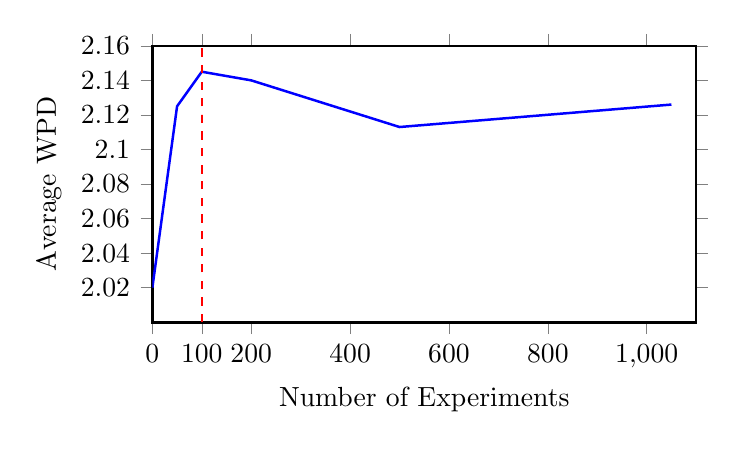
\begin{tikzpicture}
    \begin{axis}[
      width=0.7\textwidth,
      height=0.42\textwidth,
      xlabel={Number of Experiments},
      ylabel={Average WPD},
      xmin=0, xmax=1100,
      xtick={0,100,200,400,600,800,1000},
      ymin=2.00, ymax=2.16,
      ytick={2.02,2.04,2.06,2.08,2.10,2.12,2.14,2.16},
      tick align=outside,
      % grid=both,
      % grid style={line width=.2pt, draw=gray!30},
      line width=0.9pt,
      mark size=2pt
    ]
      \addplot+[mark=none] table[row sep=\\]{
        x   y \\
        0   2.02 \\
        50  2.125 \\
        100 2.145 \\
        200 2.140 \\
        500 2.113 \\
        1050 2.126 \\
      };
       % Dashed red vertical line at x = 100
      \addplot[
        red, thick, dashed,
        domain=2.00:2.16,
      ] ({100}, x);

    \end{axis}
  \end{tikzpicture}
  \caption{Average WPD vs. number of experiments. The curve flattens beyond 100 simulations, indicating convergence.}
  \label{fig:elbow_plot}
\end{figure}
% \begin{figure}[htbp]
% \centering
% 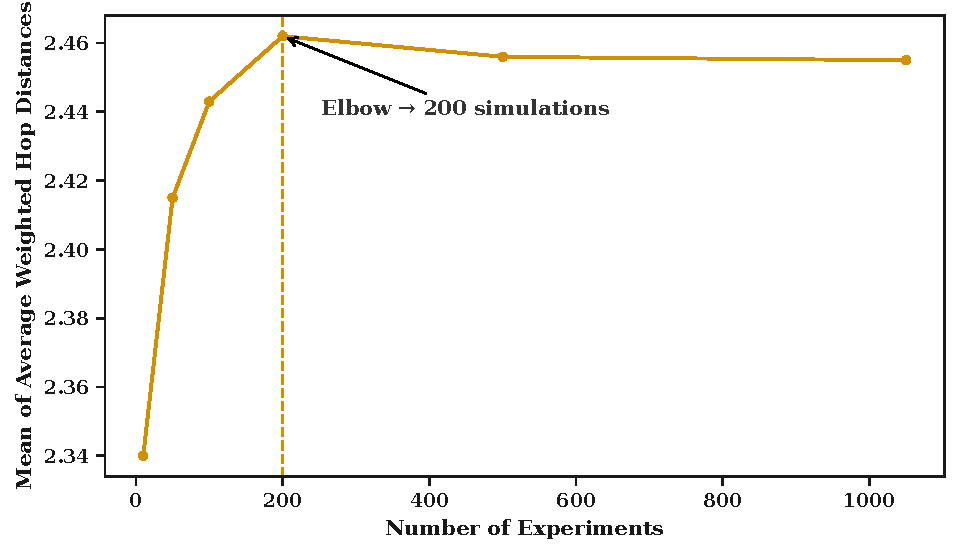
\includegraphics[width=0.85\linewidth]{images/elbow_plot_result.pdf}
% \caption{
% Elbow analysis of the mean weighted proximity distance $\mu_R$ as a function of the number of random simulations $R$. 
% The inflection point around $R = 200$ marks the threshold of convergence, beyond which additional realizations produce negligible improvement in the stability of the null distribution.
% }
% \label{fig:elbow_plot}
% \end{figure}
As summarized in Table~\ref{tab:null_wpd_stats}, the FLO \gls{dcfc} network exhibits a proximity value of 2.8820 hops, compared with a mean of 2.1272 hops across 1,050 randomized placements. Among these trials, 902 configurations (85.7\%) achieved lower \gls{wpd} values, placing the observed network in the lower tail of the null distribution and indicating that its spatial configuration underperforms relative to most random alternatives.
% A broader statistical analysis, based on 1,050 randomized experiments, yields a comparable mean of 2.1261 with a standard deviation of 0.6713. When the FLO DCFC network value is evaluated against this reference random distribution, it corresponds to a z-score of approximately 1.13 and a one-sided p-value of about 0.13, indicating that the observed deviation from random performance is not statistically significant. 
% The Kolmogorov-Smirnov test produces a p-value of 0.0012, revealing that the random metric distribution deviates from normality, and thus non-parametric methods such as permutation or bootstrap analysis provide a more reliable inference framework.
The findings indicate that the spatial arrangement of existing FLO \gls{dcfc} stations does not show strong evidence of systematic optimization when compared to randomly placed scenarios. Instead, the observed pattern seems to stem primarily from infrastructural, regulatory, and planning constraints, rather than from an efficient network-level design. 
Figure~\ref{fig:wpd_min} illustrates random charger configurations that achieve both the lowest and highest proximity metrics. This provides a visual contrast with the FLO \gls{dcfc} network and highlights the range of spatial performance outcomes that can occur under non-optimized siting conditions.
% \begin{figure}[htbp]
%     \centering
%     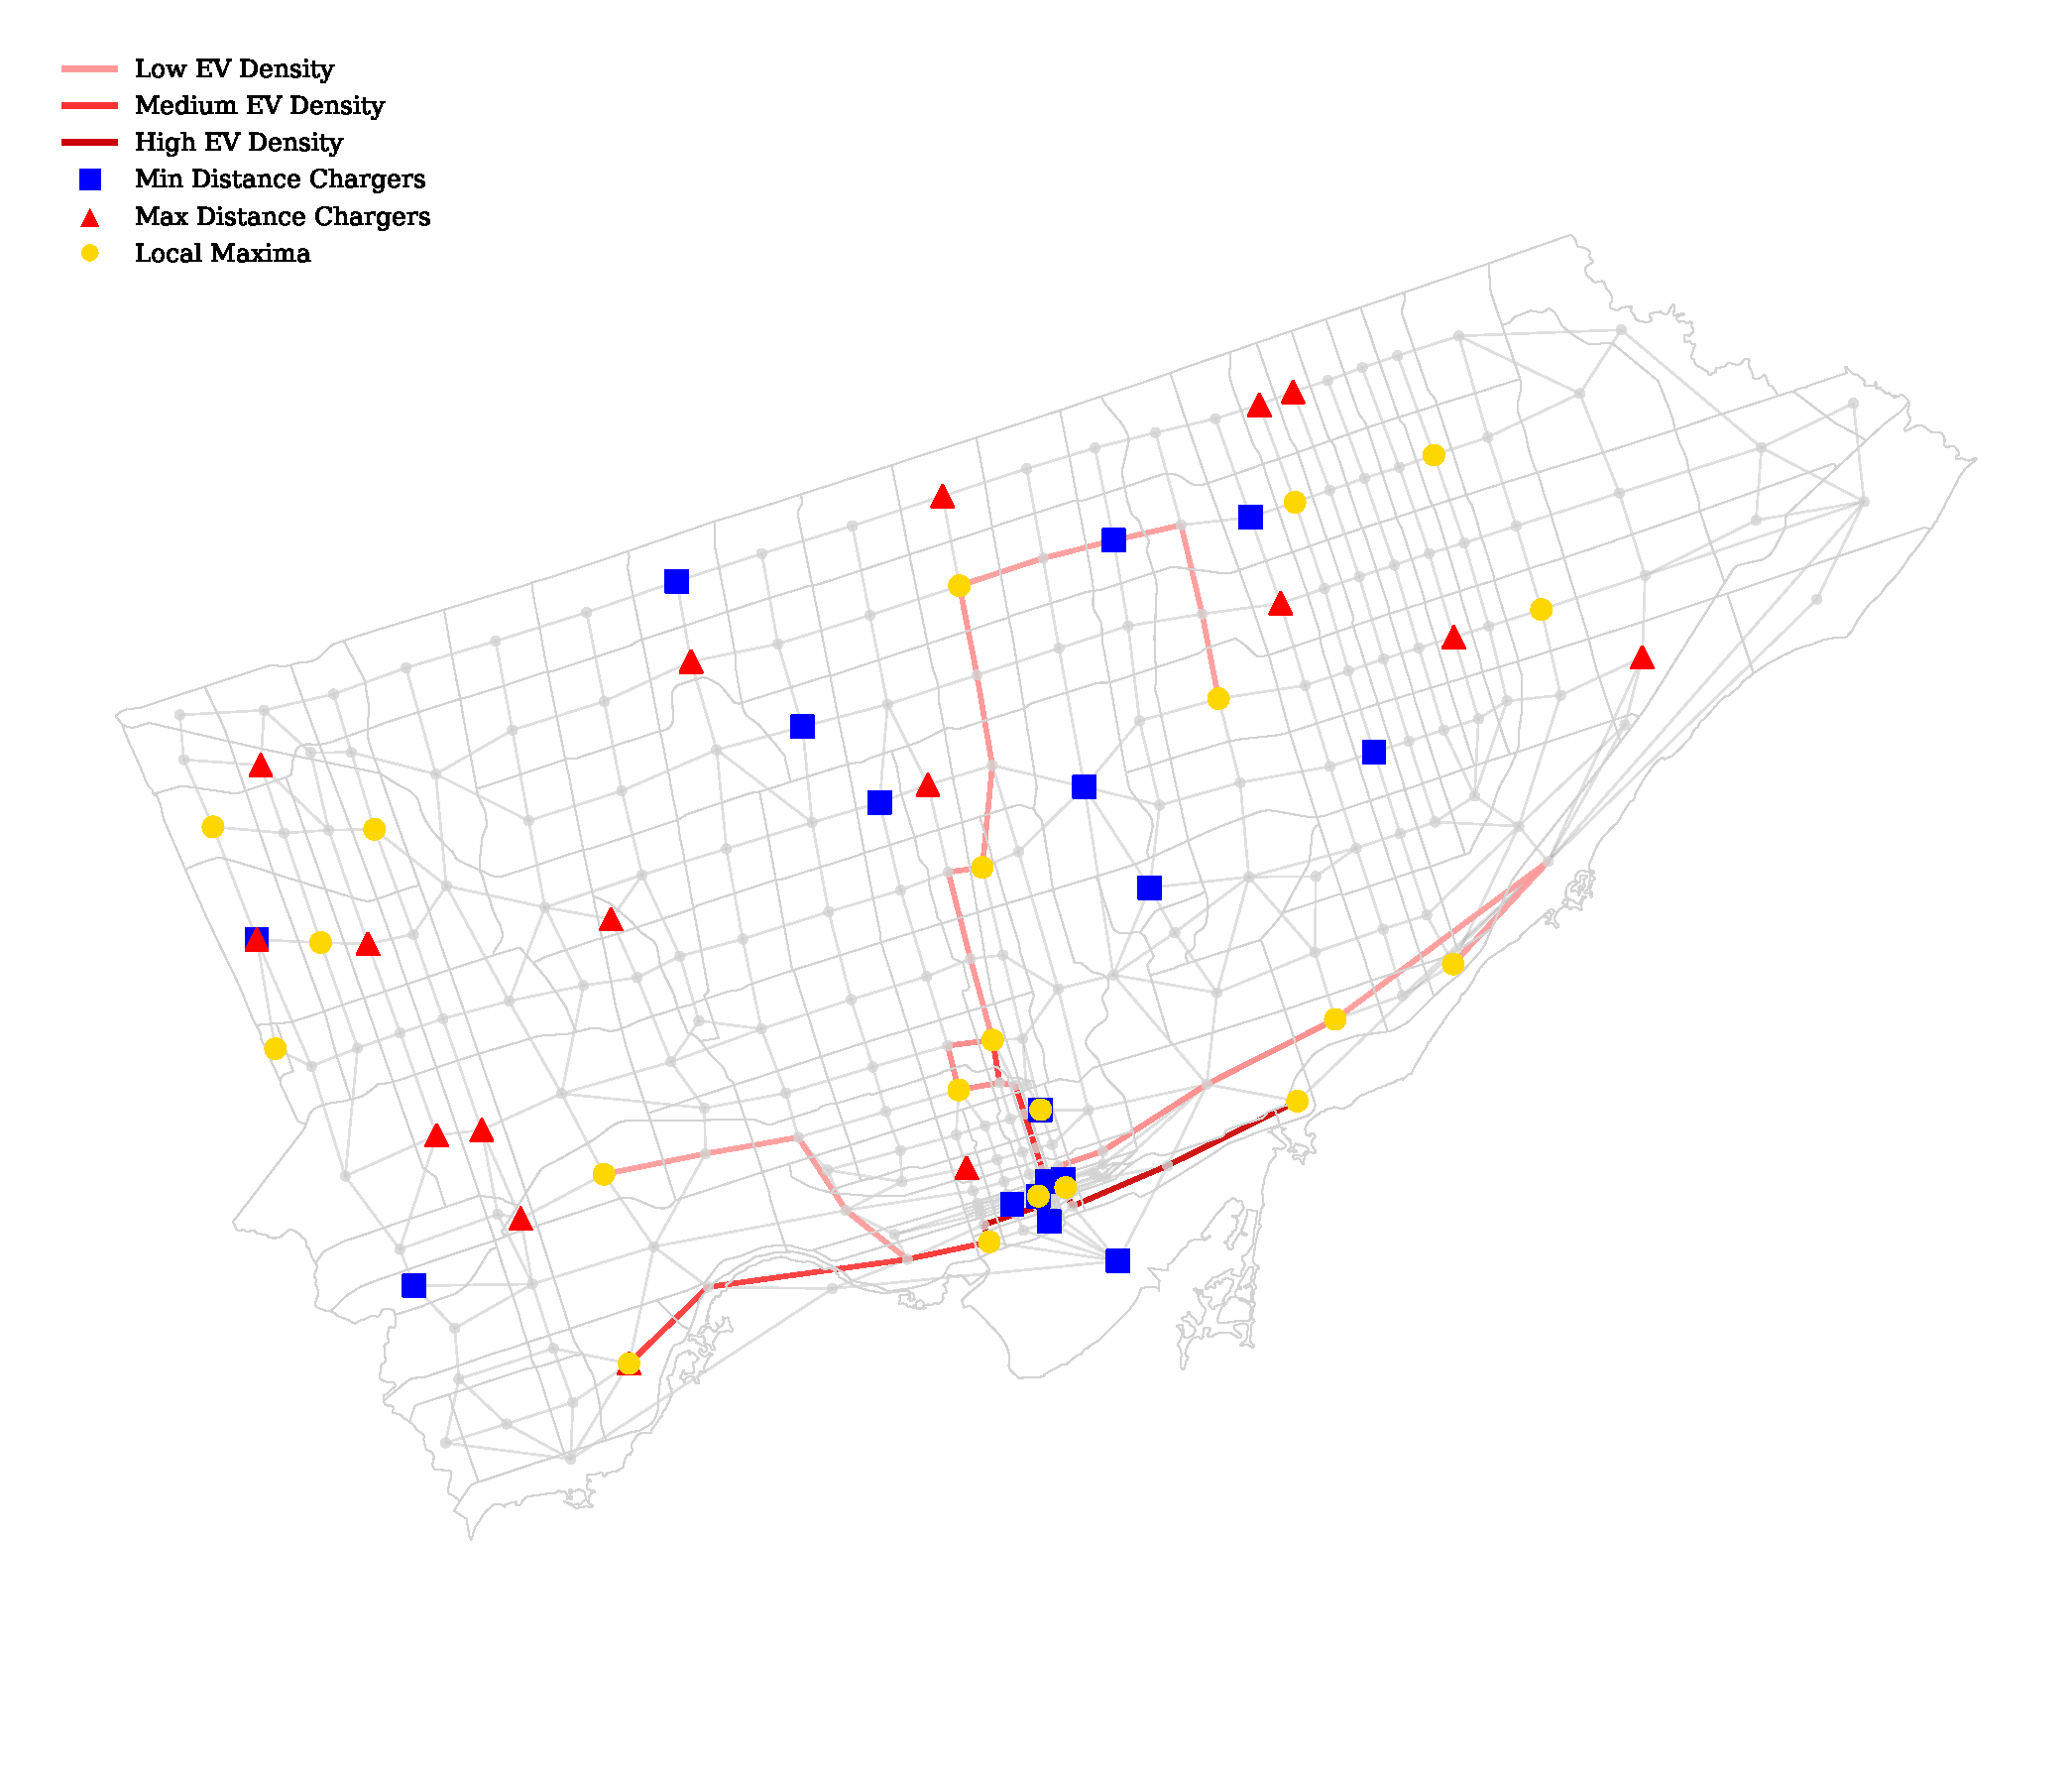
\includegraphics[width=0.85\textwidth]{images/toronto_map_random_chargers.pdf}
%     \caption{Representative random charger layouts corresponding to the lowest and highest computed proximity metrics. 
%     % These configurations provide a visual contrast to the FLO \gls{dcfc} network shown in Figure~\ref{fig:flo_dcfc_map}, 
%     % illustrating how spatial alignment between charger locations and high-activity ridge-path nodes affects the overall proximity efficiency.
%     }
%     \label{fig:wpd_min}
% \end{figure}

\begin{figure}[htbp]
    \centering
    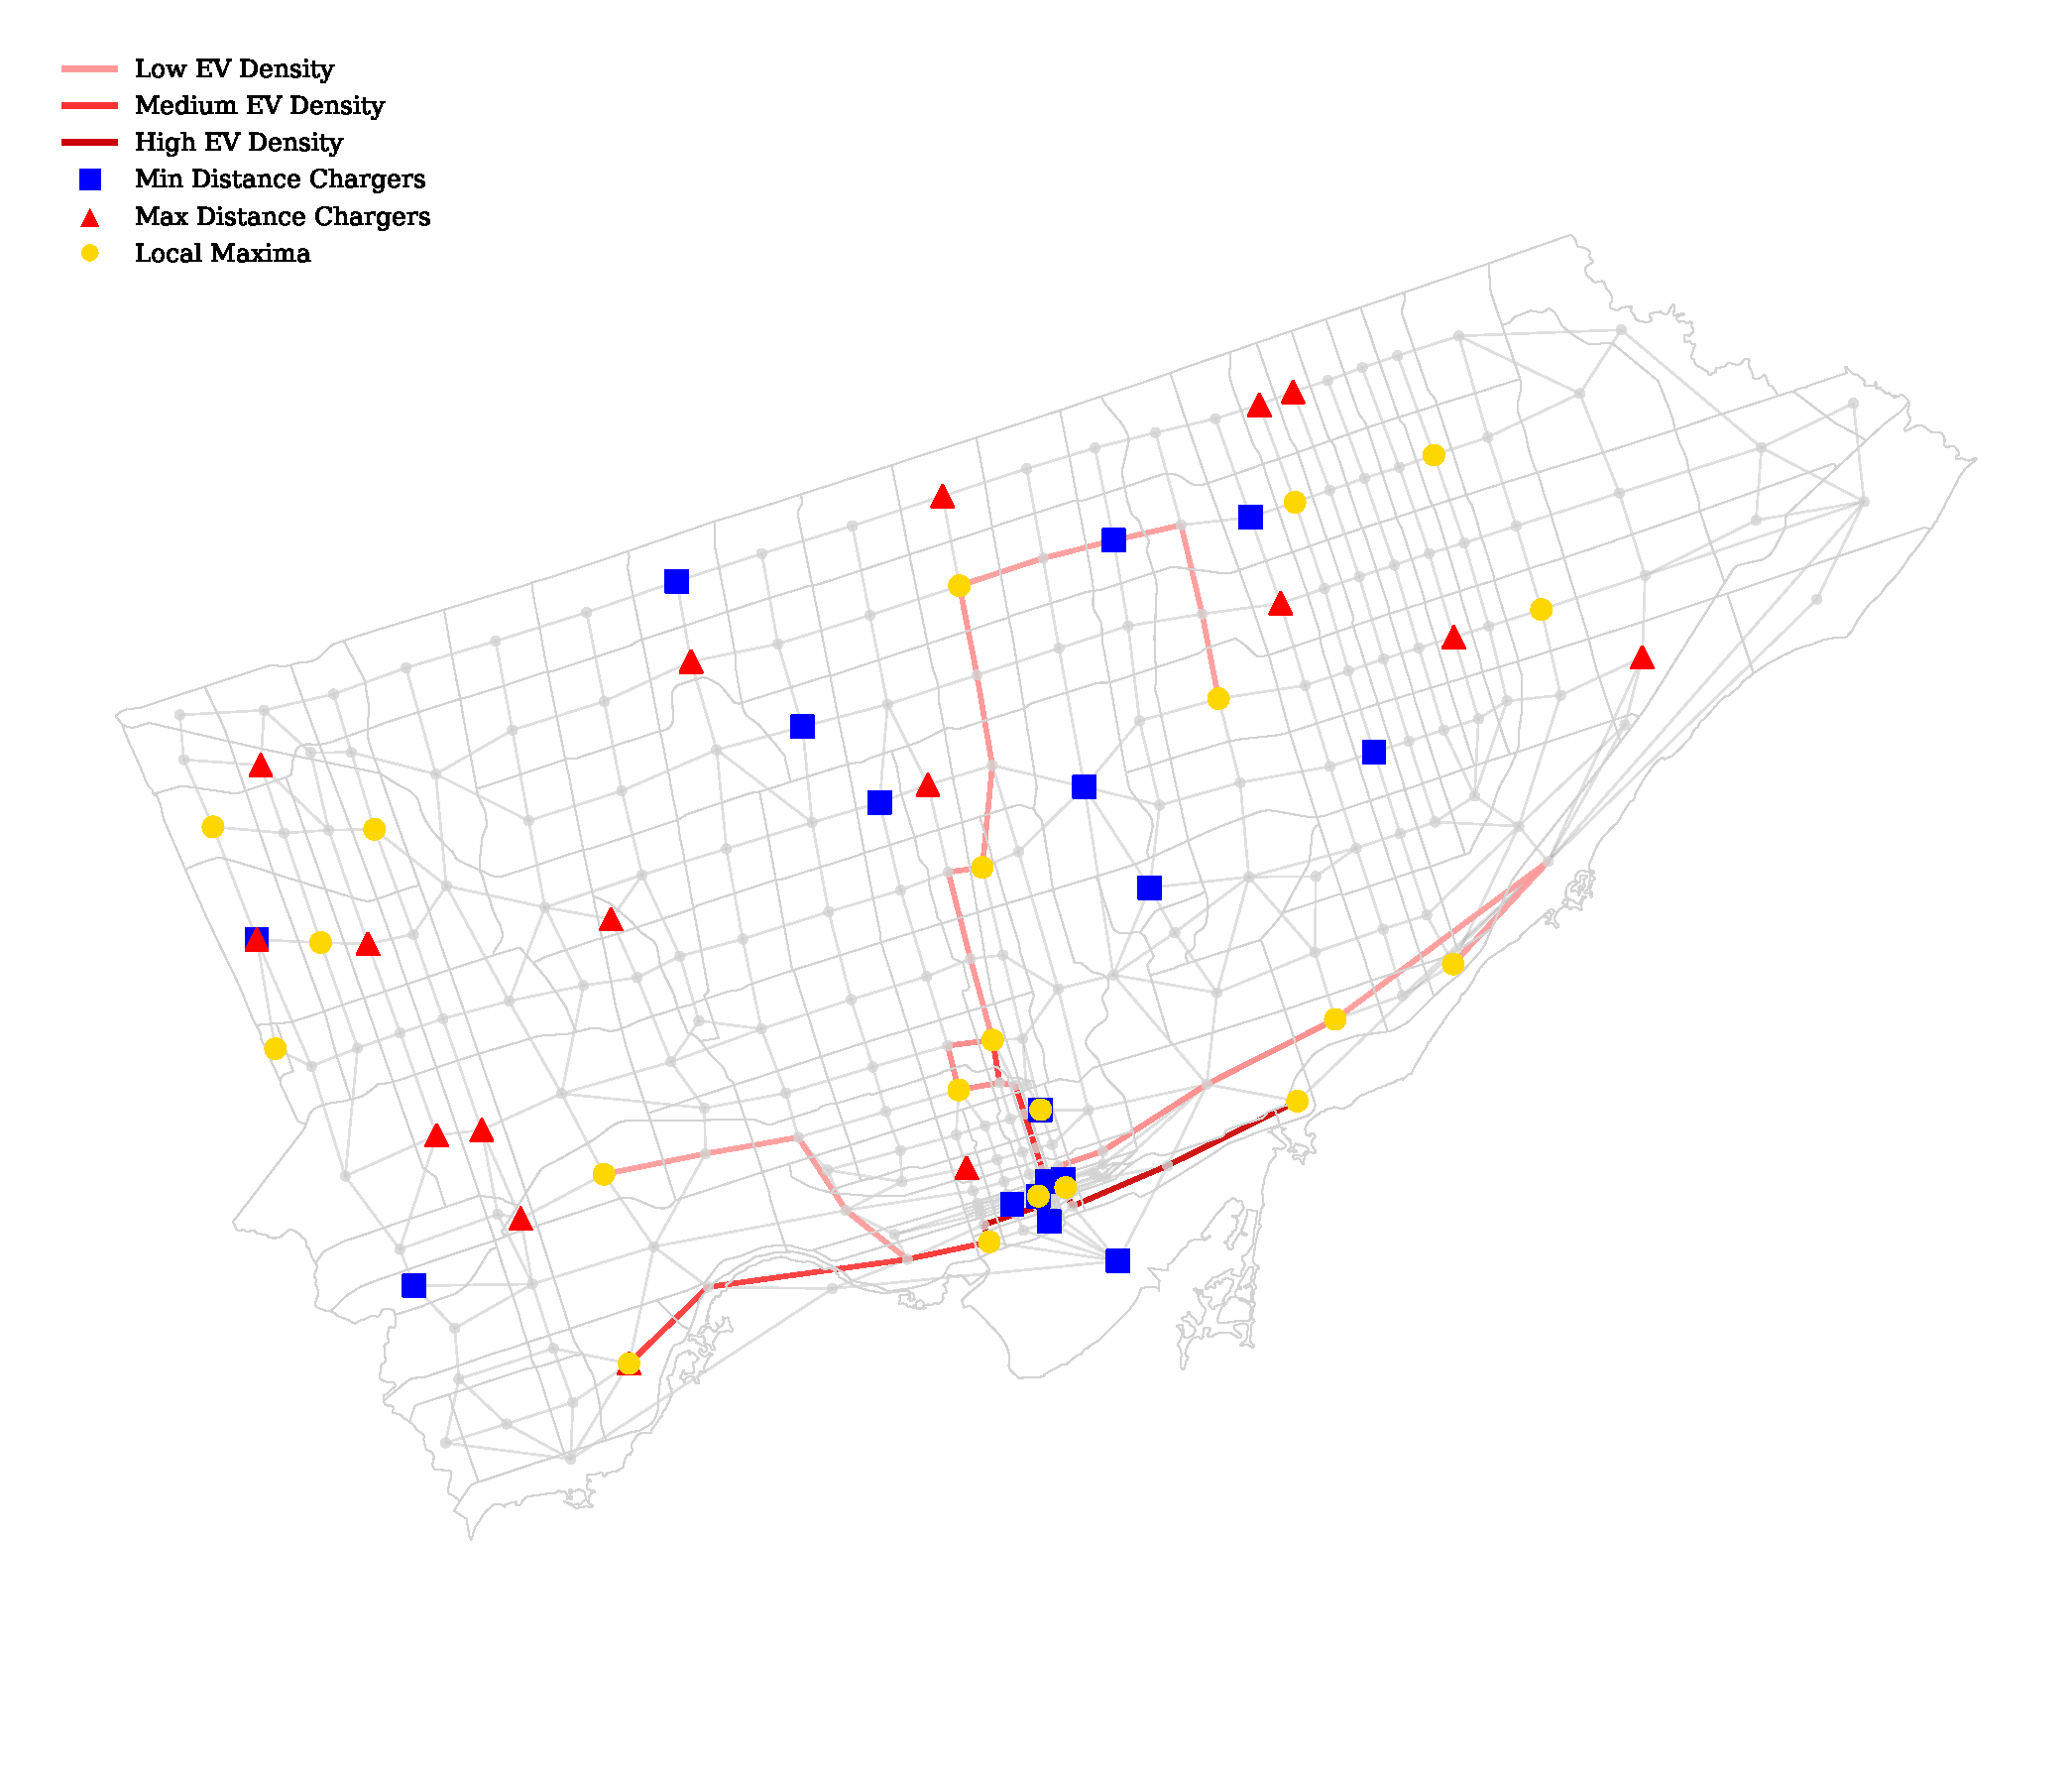
\includegraphics[width=0.7\textwidth, trim={1cm 4cm 1cm 0.8cm}, clip]{images/toronto_map_random_chargers.pdf}
    \caption{Representative random charger layouts corresponding to the lowest and highest computed proximity metrics.}
    \label{fig:wpd_min}
\end{figure}

\begin{table}[htbp]
\centering
\caption{Comprehensive Empirical Evaluation and Statistical Summary of FLO \gls{dcfc} network Proximity Performance}
\label{tab:null_wpd_stats}
\begin{tabularx}{0.9\linewidth}{@{}l>{\centering\arraybackslash}X@{}}
\toprule
\textbf{Metric} & \textbf{Value} \\
\midrule
\multicolumn{2}{@{}l}{\textbf{Empirical Evaluation}} \\[2pt]
FLO \gls{dcfc} network proximity metric (\gls{wpd}$_{\text{FLO}}$) & 2.8820 \\
Total random experiments ($R$) & 1050 \\
Random experiments with lower \gls{wpd} & 902 \\
Empirical percentile rank (\%) & 85.74 \\
Mean of random metrics ($\mathrm{E}[\mathrm{WPD}_{\text{null}}]$) & 2.1272 \\
Standard deviation ($\sigma_{\text{null}}$) & 0.6767 \\
Minimum / Maximum random \gls{wpd}$_{null}$ & 0.7471 / 4.7077 \\[4pt]
% \multicolumn{2}{@{}l}{\textbf{Statistical Inference}} \\[2pt]
% Z-score (normal approximation) & 1.13 \\
% One-sided p-value (Z-test) & 0.1312 \\
% Kolmogorov--Smirnov test p-value & 0.0012 \\
\bottomrule
\end{tabularx}
\end{table}

% -------------------------------------------------
% FIGURE 2: Demand vs. Supply scatter
% -------------------------------------------------
% \begin{figure}[H]
%   \centering
%   \includegraphics[width=0.75\linewidth, keepaspectratio]{figures/demand_supply_scatter.pdf}
%   \caption{Relationship between normalized BEV density ($\widehat{\rho}^{\mathrm{Ar}}_j$) and normalized charger capacity density ($\widehat{\rho}^{\mathrm{Ch}}_j$) across arterial zones. 
%   The dashed line indicates the best-fit regression ($r=0.47$), suggesting moderate spatial alignment between demand intensity and available charging capacity.}
%   \label{fig:demand_supply_scatter}
% \end{figure}

% -------------------------------------------------
% FIGURE 3: Null-model distribution
% -------------------------------------------------
% \begin{figure}[H]
%   \centering
%   \includegraphics[width=0.7\linewidth, keepaspectratio]{figures/null_wpd_distribution.pdf}
%   \caption{Null-model distribution of Weighted Proximity Distance (WPD) generated from 1,000 random charger configurations. 
%   The red vertical line marks the observed $\mathrm{WPD}_{\text{obs}}$, which lies in the lower tail of the null distribution ($p < 0.01$), indicating statistically significant spatial alignment between charger locations and BEV ridge-path demand.}
%   \label{fig:null_wpd}
% \end{figure}

% \subsection{Proximity Performance (Observed)}
% \label{subsec:observed_wpd}
% We compute $\mathrm{WPD}_{\mathrm{real}}$ via Eq.~\eqref{eq:wpd}. The observed value is
% \[
% \mathrm{WPD}_{\mathrm{real}} = \texttt{TODO} \quad \text{(hops)}.
% \]
% Figure~\ref{fig:nearest_assignments} illustrates nearest-charger assignments from ridge nodes.
% \begin{figure}[t]
%   \centering
%   \includegraphics[width=0.92\linewidth]{images/nearest_charger_assignments.pdf}
%   \caption{Nearest-charger assignments from ridge nodes (edges drawn along $G$).}
%   \label{fig:nearest_assignments}
% \end{figure}

% \subsection{Null Distribution and Significance}
% \label{subsec:null_significance}
% We generate $R=\texttt{TODO}$ randomized charger configurations under~\eqref{eq:null_constraints}. 
% The null mean and SD are $\mu_R=\texttt{TODO}$ and $\sigma_R=\texttt{TODO}$ (Eq.~\eqref{eq:null_stats}). 
% The empirical $p$-value (Eq.~\eqref{eq:p_perm}) is
% \[
% p_{\text{perm}} = \texttt{TODO},
% \]
% and the one-sided test~\eqref{eq:hypothesis_test} at $\alpha=0.05$ yields \texttt{Reject/Fail to reject} $H_0$.
% Figure~\ref{fig:null_hist} overlays $\mathrm{WPD}_{\mathrm{real}}$ on the null distribution; Fig.~\ref{fig:elbow_plot} shows elbow convergence of $\mu_R$.

% \begin{figure}[t]
%   \centering
%   \includegraphics[width=0.92\linewidth]{images/null_hist_wpd.pdf}
%   \caption{Null distribution of WPD and observed $\mathrm{WPD}_{\mathrm{real}}$.}
%   \label{fig:null_hist}
% \end{figure}

% \subsection{Sensitivity and Ablation Analyses}
% \label{subsec:sensitivity}
% We probe robustness to modeling choices:
% \begin{enumerate}
%   \item \textbf{$n$-hop smoothing and $\mathbf{w}$:} vary $n\in\{0,1,2,3\}$ and decay patterns; track $\mathrm{WPD}_{\mathrm{real}}$.
%   \item \textbf{Ridge parameters ($\eta,\alpha$):} sweep drop tolerance and max length; report ridge coverage and WPD.
%   \item \textbf{Distance model:} hop vs.\ Euclidean; report $\Delta$WPD.
%   \item \textbf{Supply weighting:} with/without $\widehat{\rho}^{\mathrm{Ch}}$ (capacity-neutral).
%   \item \textbf{Dasymetric refinements:} area vs.\ dwelling/land-use/road-length weights (Appendix sensitivity).
% \end{enumerate}

% \begin{table}[t]
%   \centering
%   \caption{Sensitivity of $\mathrm{WPD}_{\mathrm{real}}$ across modeling choices.}
%   \label{tab:sensitivity}
%   \begin{tabular}{l r r r}
%     \toprule
%     Setting & Param(s) & $\mathrm{WPD}_{\mathrm{real}}$ & $\Delta$ (\%) \\
%     \midrule
%     Baseline & $n=\texttt{TODO}$, $m=\texttt{TODO}$ & \texttt{TODO} & -- \\
%     Hop $\to$ Euclid & -- & \texttt{TODO} & \texttt{TODO} \\
%     No capacity wgt & $w_s\!\to\!1$ & \texttt{TODO} & \texttt{TODO} \\
%     \bottomrule
%   \end{tabular}
% \end{table}

% \subsection{Targeted Corridor Diagnostics (Actionable Gaps)}
% \label{subsec:diagnostics}
% We identify ridge nodes with largest $d_G(v_j,c^*(v_j))$ under high demand $\widehat{\rho}^{\mathrm{Ar}}_j$ and low supply $\widehat{\rho}^{\mathrm{Ch}}$.
% Figure~\ref{fig:gap_map} maps top decile gaps; Table~\ref{tab:corridor_candidates} lists candidate corridors for prioritization.

% \begin{figure}[t]
%   \centering
%   \includegraphics[width=0.92\linewidth]{images/gap_hotspots_map.pdf}
%   \caption{High-demand / low-supply proximity gaps along ridge corridors.}
%   \label{fig:gap_map}
% \end{figure}

% \begin{table}[t]
%   \centering
%   \caption{Candidate corridors for incremental fast-charger deployment.}
%   \label{tab:corridor_candidates}
%   \begin{tabular}{l r r r}
%     \toprule
%     Corridor & Mean demand & Mean supply & Mean distance (hops) \\
%     \midrule
%     \texttt{TODO} & \texttt{TODO} & \texttt{TODO} & \texttt{TODO} \\
%     \bottomrule
%   \end{tabular}
% \end{table}

% \subsection{Computation and Reproducibility}
% \label{subsec:compute_repro}
% Total runtime: \texttt{TODO} (R=\texttt{TODO}); peak memory: \texttt{TODO}.
% Code and parameter files are archived at \texttt{TODO-Repository} with fixed random seeds.
% % TODO: add DOI/Zenodo link if applicable.


\section{Conclusion}
\label{sec:conclusion}
This study has redefined how spatial structure is conceptualized in \gls{bev} \gls{fc} planning by introducing a meso-level, mobility-based framework grounded in arterial mobility network topology. Through the derivation of 234 arterial zones in Toronto, the proposed schema bridges the disconnect between administrative or statical zoning schema and the dynamic nature of \gls{bev} movement. By redistributing ownership data from \glspl{fsa} to these arterial units, the framework constructs a demand field that is directly anchored in urban mobility. Ridge-path extraction then identifies contiguous high-activity corridor zones that represent the structural backbone of BEV activity, while a graph-based proximity analysis quantifies how effectively current infrastructure serves these activity ridges.

Statical benchmarking of Toronto’s existing 17 FLO \gls{dcfc} stations against 1,050 randomized configurations revealed that 85.7\% of random networks achieved shorter weighted proximity distances. This outcome demonstrates that the current network configuration performs no better than random spatial allocation, indicating the absence of systematic spatial optimization in current deployment practices. Despite partial coincidence with major activity zones, the FLO network’s overall alignment with \gls{bev} demand remains weak, highlighting the need for an evidence-based, mobility-aware siting strategy.
Conceptually, the study contributes a scalable, interpretable, and data-efficient foundation for meso-level planning. By coupling arterial-mobility zoning with graph-theoretic analysis, the framework enables multi-criteria evaluation of accessibility, redundancy, and spatial equity without requiring detailed traffic or behavioral datasets. It advances meso-level planning beyond static administrative or grid-based methods, providing a transferable analytical layer that can inform both early-stage infrastructure rollouts and subsequent micro-level optimization models.

Practically, the findings underscore a critical policy implication: current \gls{fc} infrastructure network expansions must evolve from opportunistic placement toward mobility-aligned design. Incorporating arterial road structures into planning can ensure that public and private deployments converge toward regions of highest activity and accessibility. The framework also supports coordination among network operators, enabling municipalities to integrate equity and resilience targets within spatial optimization strategies.
In sum, this research establishes a methodological bridge between macro-level electrification objectives and micro-scale siting models. By anchoring meso-level analysis in the geometry of major urban mobility rather than in administratively or statistically convenient boundaries, it lays a foundation for next-generation planning frameworks that align \gls{bev} charging infrastructure with the actual spatial topology of urban movement.



% This study advances a mobility-based framework for understanding and planning \gls{bev} \gls{fc} infrastructure through the development of a new zoning schema aligned with major arterial roads. The approach maps \gls{bev} ownership counts from administrative units onto these arterial zones, extracts ridge paths from the arterial adjacency graph, and benchmarks network alignment using graph-based proximity metrics. The ridge-extraction pipeline, initiated from local maxima of smoothed \gls{bev} densities , as illustrated in Figure~\ref{fig:local_maxima_map}, reveals distinct, high-activity corridor zones that represent concentrated demand backbones within the urban fabric. The union of ridge-paths' nodes delineates a compact and interpretable backbone of \gls{bev} activity.

% This mobility-based zoning schema complements conventional zoning-based planning by explicitly representing the chain structure of urban \gls{bev} activity and the hop-wise accessibility between activity ridges and charging supply nodes. Results indicate that incremental siting along identified ridge spines can yield pronounced gains in proximity efficiency, particularly where short, high-intensity links integrate into broader corridor networks. Furthermore, this study introduces a new evaluation method based on constructing a null distribution that preserves the fixed number of charger stations and ports, reflecting either existing \gls{dcfc} networks or planned deployments. This enables benchmarking the efficiency of observed or planned networks against randomized charger placements, thereby quantifying how effectively the actual configurations serve \gls{bev} charging demand relative to chance.

% These findings indicate that the existing FLO \gls{dcfc} network does not exhibit spatial optimization relative to potential configurations of comparable scale and capacity. Although charger deployment shows concentration along several \gls{bev}-intensive arterial corridor-zones, the overall placement does not outperform randomized alternatives, revealing a clear gap between the current infrastructure pattern and an optimized spatial configuration. This discrepancy underscores an important research direction-investigating the sources of this gap and the contextual parameters that influence charger siting decisions. Potential contributing factors include business-driven placement priorities, infrastructural and zoning constraints, the coexistence of other \gls{dcfc} networks, and limited coordination among service providers. Understanding these influences is essential for developing data-driven, system-level siting strategies that better align charging supply with \gls{bev} demand along urban arterial corridor-zones.
% Several simplifying assumptions remain. Port power ratings were standardized where station-level specifications were unavailable, potentially understating spatial heterogeneity in delivered capacity. Static BEV density surfaces do not capture temporal fluctuations in activity, and the hop-based metric abstracts away operational constraints such as queuing, power-sharing, and distribution feeder limits. Finally, proximity benchmarking relies on a specific null model and a fixed set of ridge hyperparameters $(L,\eta)$. In sum, the ridge-path lens offers a concise and interpretable backbone of BEV activity that aligns with, but is not yet fully served by, the existing FLO DCFC network. Targeted expansions along undersupplied ridge segments, guided by proximity benchmarks and the future extensions outlined above, present a viable pathway toward higher utilization, equitable access, and grid-aware electrification outcomes.

\section{Future directions}
Future work will extend the proposed meso-level framework along three complementary dimensions: methodological refinement, data integration, and policy application.
From a methodological standpoint, subsequent studies should examine the sensitivity of ridge-path extraction to hyperparameters such as hop distance, drop tolerance, and smoothing weights, as well as explore alternative definitions of adjacency that incorporate traffic flow intensity or functional road hierarchy. The null-distribution benchmarking framework can be expanded to account for spatial clustering, land-use constraints, and power-grid limitations, thereby producing more realistic counterfactual baselines for evaluating charger-activity alignment.

In terms of data integration, future research should incorporate temporal dimensions of \gls{bev} usage, such as diurnal and seasonal charging patterns, by leveraging real charging-session data and mobility traces. Combining these dynamic demand profiles with feeder capacity and transformer headroom models would enable joint optimization of accessibility and grid impact. Emerging graph-learning techniques, including graph neural networks and spatial-temporal embedding models, offer promising avenues for forecasting corridor-level demand and optimizing charger placement under uncertainty.
At the policy level, the framework could support multi-objective planning that simultaneously addresses proximity, equity, resilience, and cost. Comparative case studies across diverse urban forms and governance contexts would help establish typologies of corridor-based \gls{bev} activity and identify transferable siting principles. Ultimately, these extensions aim to transform the proposed framework into a standardized, data-efficient planning tool that informs coordinated, mobility-aligned deployment of \gls{fc} infrastructure in support of large-scale transportation electrification.

% Future research will extend the ridge extraction and proximity analysis framework to incorporate temporal dynamics in \gls{bev} activity. This includes modeling diurnal, weekly, and seasonal variations using charging-session logs and mobility traces to capture time-resolved demand patterns. Nominal port powers will be replaced by site-level ratings with dynamic derating models, while corridor accessibility will be coupled with feeder and transformer headroom to jointly optimize siting and grid impact.

% Further investigations will systematically assess sensitivity to ridge hyperparameters $(L, \eta)$, smoothing choices, and adjacency definitions. Alternative null models that preserve spatial clustering or land-use constraints will be explored to provide more realistic baselines for evaluating spatial performance metrics.
% The WPD metric will be embedded within a broader set of objectives that balance proximity, equity, resiliency, and cost. This multi-objective formulation will enable Pareto analyses for siting strategies that simultaneously serve dense urban cores and underserved peripheral corridors.

% Uncertainty in proximity gains under demand and supply perturbations will be quantified using probabilistic or scenario-based methods. Where feasible, natural experiments or phased deployments will be leveraged to evaluate causal impacts of new charging infrastructure on utilization and accessibility outcomes.
% Validation across diverse urban forms and transportation network topologies will test the transferability of the mobility-based methodology and support the development of typologies that link ridge structures with accessibility and utilization outcomes. Additionally, emerging graph-based learning methods, such as graph neural networks, will be explored to forecast corridor-level demand and recommend capacity expansions under constrained budgets and grid limitations.

% Finally, the research will focus on identifying underlying factors contributing to the observed gap between the existing and optimized fast-charger network configurations. This includes analyzing how business-driven siting priorities, infrastructural and zoning constraints, and the presence of competing \gls{dcfc} networks shape the spatial distribution of chargers. Understanding these parameters will support coordinated, data-driven siting strategies that align charging supply with \gls{bev} activity along urban arterial corridors.


% ----------------------
% References
% ----------------------
% \bibliography{ref}



\nocite{*}
\bibliographystyle{IEEEtran}
\bibliography{references,refs_chapter7}

\end{document}
